% Options for packages loaded elsewhere
\PassOptionsToPackage{unicode}{hyperref}
\PassOptionsToPackage{hyphens}{url}
\PassOptionsToPackage{dvipsnames,svgnames,x11names}{xcolor}
%
\documentclass[
  a4paper,
  DIV=11,
  numbers=noendperiod]{scrartcl}

\usepackage{amsmath,amssymb}
\usepackage{iftex}
\ifPDFTeX
  \usepackage[T1]{fontenc}
  \usepackage[utf8]{inputenc}
  \usepackage{textcomp} % provide euro and other symbols
\else % if luatex or xetex
  \usepackage{unicode-math}
  \defaultfontfeatures{Scale=MatchLowercase}
  \defaultfontfeatures[\rmfamily]{Ligatures=TeX,Scale=1}
\fi
\usepackage{lmodern}
\ifPDFTeX\else  
    % xetex/luatex font selection
\fi
% Use upquote if available, for straight quotes in verbatim environments
\IfFileExists{upquote.sty}{\usepackage{upquote}}{}
\IfFileExists{microtype.sty}{% use microtype if available
  \usepackage[]{microtype}
  \UseMicrotypeSet[protrusion]{basicmath} % disable protrusion for tt fonts
}{}
\makeatletter
\@ifundefined{KOMAClassName}{% if non-KOMA class
  \IfFileExists{parskip.sty}{%
    \usepackage{parskip}
  }{% else
    \setlength{\parindent}{0pt}
    \setlength{\parskip}{6pt plus 2pt minus 1pt}}
}{% if KOMA class
  \KOMAoptions{parskip=half}}
\makeatother
\usepackage{xcolor}
\setlength{\emergencystretch}{3em} % prevent overfull lines
\setcounter{secnumdepth}{5}
% Make \paragraph and \subparagraph free-standing
\makeatletter
\ifx\paragraph\undefined\else
  \let\oldparagraph\paragraph
  \renewcommand{\paragraph}{
    \@ifstar
      \xxxParagraphStar
      \xxxParagraphNoStar
  }
  \newcommand{\xxxParagraphStar}[1]{\oldparagraph*{#1}\mbox{}}
  \newcommand{\xxxParagraphNoStar}[1]{\oldparagraph{#1}\mbox{}}
\fi
\ifx\subparagraph\undefined\else
  \let\oldsubparagraph\subparagraph
  \renewcommand{\subparagraph}{
    \@ifstar
      \xxxSubParagraphStar
      \xxxSubParagraphNoStar
  }
  \newcommand{\xxxSubParagraphStar}[1]{\oldsubparagraph*{#1}\mbox{}}
  \newcommand{\xxxSubParagraphNoStar}[1]{\oldsubparagraph{#1}\mbox{}}
\fi
\makeatother

\usepackage{color}
\usepackage{fancyvrb}
\newcommand{\VerbBar}{|}
\newcommand{\VERB}{\Verb[commandchars=\\\{\}]}
\DefineVerbatimEnvironment{Highlighting}{Verbatim}{commandchars=\\\{\}}
% Add ',fontsize=\small' for more characters per line
\usepackage{framed}
\definecolor{shadecolor}{RGB}{241,243,245}
\newenvironment{Shaded}{\begin{snugshade}}{\end{snugshade}}
\newcommand{\AlertTok}[1]{\textcolor[rgb]{0.68,0.00,0.00}{#1}}
\newcommand{\AnnotationTok}[1]{\textcolor[rgb]{0.37,0.37,0.37}{#1}}
\newcommand{\AttributeTok}[1]{\textcolor[rgb]{0.40,0.45,0.13}{#1}}
\newcommand{\BaseNTok}[1]{\textcolor[rgb]{0.68,0.00,0.00}{#1}}
\newcommand{\BuiltInTok}[1]{\textcolor[rgb]{0.00,0.23,0.31}{#1}}
\newcommand{\CharTok}[1]{\textcolor[rgb]{0.13,0.47,0.30}{#1}}
\newcommand{\CommentTok}[1]{\textcolor[rgb]{0.37,0.37,0.37}{#1}}
\newcommand{\CommentVarTok}[1]{\textcolor[rgb]{0.37,0.37,0.37}{\textit{#1}}}
\newcommand{\ConstantTok}[1]{\textcolor[rgb]{0.56,0.35,0.01}{#1}}
\newcommand{\ControlFlowTok}[1]{\textcolor[rgb]{0.00,0.23,0.31}{\textbf{#1}}}
\newcommand{\DataTypeTok}[1]{\textcolor[rgb]{0.68,0.00,0.00}{#1}}
\newcommand{\DecValTok}[1]{\textcolor[rgb]{0.68,0.00,0.00}{#1}}
\newcommand{\DocumentationTok}[1]{\textcolor[rgb]{0.37,0.37,0.37}{\textit{#1}}}
\newcommand{\ErrorTok}[1]{\textcolor[rgb]{0.68,0.00,0.00}{#1}}
\newcommand{\ExtensionTok}[1]{\textcolor[rgb]{0.00,0.23,0.31}{#1}}
\newcommand{\FloatTok}[1]{\textcolor[rgb]{0.68,0.00,0.00}{#1}}
\newcommand{\FunctionTok}[1]{\textcolor[rgb]{0.28,0.35,0.67}{#1}}
\newcommand{\ImportTok}[1]{\textcolor[rgb]{0.00,0.46,0.62}{#1}}
\newcommand{\InformationTok}[1]{\textcolor[rgb]{0.37,0.37,0.37}{#1}}
\newcommand{\KeywordTok}[1]{\textcolor[rgb]{0.00,0.23,0.31}{\textbf{#1}}}
\newcommand{\NormalTok}[1]{\textcolor[rgb]{0.00,0.23,0.31}{#1}}
\newcommand{\OperatorTok}[1]{\textcolor[rgb]{0.37,0.37,0.37}{#1}}
\newcommand{\OtherTok}[1]{\textcolor[rgb]{0.00,0.23,0.31}{#1}}
\newcommand{\PreprocessorTok}[1]{\textcolor[rgb]{0.68,0.00,0.00}{#1}}
\newcommand{\RegionMarkerTok}[1]{\textcolor[rgb]{0.00,0.23,0.31}{#1}}
\newcommand{\SpecialCharTok}[1]{\textcolor[rgb]{0.37,0.37,0.37}{#1}}
\newcommand{\SpecialStringTok}[1]{\textcolor[rgb]{0.13,0.47,0.30}{#1}}
\newcommand{\StringTok}[1]{\textcolor[rgb]{0.13,0.47,0.30}{#1}}
\newcommand{\VariableTok}[1]{\textcolor[rgb]{0.07,0.07,0.07}{#1}}
\newcommand{\VerbatimStringTok}[1]{\textcolor[rgb]{0.13,0.47,0.30}{#1}}
\newcommand{\WarningTok}[1]{\textcolor[rgb]{0.37,0.37,0.37}{\textit{#1}}}

\providecommand{\tightlist}{%
  \setlength{\itemsep}{0pt}\setlength{\parskip}{0pt}}\usepackage{longtable,booktabs,array}
\usepackage{calc} % for calculating minipage widths
% Correct order of tables after \paragraph or \subparagraph
\usepackage{etoolbox}
\makeatletter
\patchcmd\longtable{\par}{\if@noskipsec\mbox{}\fi\par}{}{}
\makeatother
% Allow footnotes in longtable head/foot
\IfFileExists{footnotehyper.sty}{\usepackage{footnotehyper}}{\usepackage{footnote}}
\makesavenoteenv{longtable}
\usepackage{graphicx}
\makeatletter
\newsavebox\pandoc@box
\newcommand*\pandocbounded[1]{% scales image to fit in text height/width
  \sbox\pandoc@box{#1}%
  \Gscale@div\@tempa{\textheight}{\dimexpr\ht\pandoc@box+\dp\pandoc@box\relax}%
  \Gscale@div\@tempb{\linewidth}{\wd\pandoc@box}%
  \ifdim\@tempb\p@<\@tempa\p@\let\@tempa\@tempb\fi% select the smaller of both
  \ifdim\@tempa\p@<\p@\scalebox{\@tempa}{\usebox\pandoc@box}%
  \else\usebox{\pandoc@box}%
  \fi%
}
% Set default figure placement to htbp
\def\fps@figure{htbp}
\makeatother
% definitions for citeproc citations
\NewDocumentCommand\citeproctext{}{}
\NewDocumentCommand\citeproc{mm}{%
  \begingroup\def\citeproctext{#2}\cite{#1}\endgroup}
\makeatletter
 % allow citations to break across lines
 \let\@cite@ofmt\@firstofone
 % avoid brackets around text for \cite:
 \def\@biblabel#1{}
 \def\@cite#1#2{{#1\if@tempswa , #2\fi}}
\makeatother
\newlength{\cslhangindent}
\setlength{\cslhangindent}{1.5em}
\newlength{\csllabelwidth}
\setlength{\csllabelwidth}{3em}
\newenvironment{CSLReferences}[2] % #1 hanging-indent, #2 entry-spacing
 {\begin{list}{}{%
  \setlength{\itemindent}{0pt}
  \setlength{\leftmargin}{0pt}
  \setlength{\parsep}{0pt}
  % turn on hanging indent if param 1 is 1
  \ifodd #1
   \setlength{\leftmargin}{\cslhangindent}
   \setlength{\itemindent}{-1\cslhangindent}
  \fi
  % set entry spacing
  \setlength{\itemsep}{#2\baselineskip}}}
 {\end{list}}
\usepackage{calc}
\newcommand{\CSLBlock}[1]{\hfill\break\parbox[t]{\linewidth}{\strut\ignorespaces#1\strut}}
\newcommand{\CSLLeftMargin}[1]{\parbox[t]{\csllabelwidth}{\strut#1\strut}}
\newcommand{\CSLRightInline}[1]{\parbox[t]{\linewidth - \csllabelwidth}{\strut#1\strut}}
\newcommand{\CSLIndent}[1]{\hspace{\cslhangindent}#1}

\KOMAoption{captions}{tableheading}
\makeatletter
\@ifpackageloaded{tcolorbox}{}{\usepackage[skins,breakable]{tcolorbox}}
\@ifpackageloaded{fontawesome5}{}{\usepackage{fontawesome5}}
\definecolor{quarto-callout-color}{HTML}{909090}
\definecolor{quarto-callout-note-color}{HTML}{0758E5}
\definecolor{quarto-callout-important-color}{HTML}{CC1914}
\definecolor{quarto-callout-warning-color}{HTML}{EB9113}
\definecolor{quarto-callout-tip-color}{HTML}{00A047}
\definecolor{quarto-callout-caution-color}{HTML}{FC5300}
\definecolor{quarto-callout-color-frame}{HTML}{acacac}
\definecolor{quarto-callout-note-color-frame}{HTML}{4582ec}
\definecolor{quarto-callout-important-color-frame}{HTML}{d9534f}
\definecolor{quarto-callout-warning-color-frame}{HTML}{f0ad4e}
\definecolor{quarto-callout-tip-color-frame}{HTML}{02b875}
\definecolor{quarto-callout-caution-color-frame}{HTML}{fd7e14}
\makeatother
\makeatletter
\@ifpackageloaded{caption}{}{\usepackage{caption}}
\AtBeginDocument{%
\ifdefined\contentsname
  \renewcommand*\contentsname{Table of contents}
\else
  \newcommand\contentsname{Table of contents}
\fi
\ifdefined\listfigurename
  \renewcommand*\listfigurename{List of Figures}
\else
  \newcommand\listfigurename{List of Figures}
\fi
\ifdefined\listtablename
  \renewcommand*\listtablename{List of Tables}
\else
  \newcommand\listtablename{List of Tables}
\fi
\ifdefined\figurename
  \renewcommand*\figurename{Figure}
\else
  \newcommand\figurename{Figure}
\fi
\ifdefined\tablename
  \renewcommand*\tablename{Table}
\else
  \newcommand\tablename{Table}
\fi
}
\@ifpackageloaded{float}{}{\usepackage{float}}
\floatstyle{ruled}
\@ifundefined{c@chapter}{\newfloat{codelisting}{h}{lop}}{\newfloat{codelisting}{h}{lop}[chapter]}
\floatname{codelisting}{Listing}
\newcommand*\listoflistings{\listof{codelisting}{List of Listings}}
\makeatother
\makeatletter
\makeatother
\makeatletter
\@ifpackageloaded{caption}{}{\usepackage{caption}}
\@ifpackageloaded{subcaption}{}{\usepackage{subcaption}}
\makeatother
\newcounter{quartocalloutnteno}
\newcommand{\quartocalloutnte}[1]{\refstepcounter{quartocalloutnteno}\label{#1}}
\newcounter{quartocalloutimpno}
\newcommand{\quartocalloutimp}[1]{\refstepcounter{quartocalloutimpno}\label{#1}}

\ifLuaTeX
\usepackage[bidi=basic]{babel}
\else
\usepackage[bidi=default]{babel}
\fi
\babelprovide[main,import]{american}
% get rid of language-specific shorthands (see #6817):
\let\LanguageShortHands\languageshorthands
\def\languageshorthands#1{}
\ifLuaTeX
  \usepackage[english]{selnolig} % disable illegal ligatures
\fi
\usepackage{bookmark}

\IfFileExists{xurl.sty}{\usepackage{xurl}}{} % add URL line breaks if available
\urlstyle{same} % disable monospaced font for URLs
\hypersetup{
  pdftitle={Analog Circuit Design},
  pdfauthor={Harald Pretl; Michael Koefinger; Simon Dorrer},
  pdflang={en-US},
  colorlinks=true,
  linkcolor={blue},
  filecolor={Maroon},
  citecolor={Blue},
  urlcolor={Blue},
  pdfcreator={LaTeX via pandoc}}


\title{Analog Circuit Design}
\author{Harald Pretl \and Michael Koefinger \and Simon Dorrer}
\date{2025-01-14}

\begin{document}
\maketitle

\renewcommand*\contentsname{Table of contents}
{
\hypersetup{linkcolor=}
\setcounter{tocdepth}{3}
\tableofcontents
}

\section{Introduction}\label{sec-intro}

This is the material for an intermediate-level MOSFET analog circuit
design course, held at JKU under course number 336.009 (``KV Analoge
Schaltungstechnik'').

The course makes heavy use of circuit simulation, using \textbf{Xschem}
for schematic entry and \textbf{ngspice} for simulation. The 130nm CMOS
technology \textbf{SG13G2} from IHP Microelectronics is used.

Tools and PDK are integrated in the \textbf{IIC-OSIC-TOOLS} Docker
image, which will be used during the coursework.

\begin{tcolorbox}[enhanced jigsaw, breakable, arc=.35mm, colbacktitle=quarto-callout-important-color!10!white, toprule=.15mm, left=2mm, toptitle=1mm, bottomtitle=1mm, opacityback=0, rightrule=.15mm, opacitybacktitle=0.6, titlerule=0mm, colback=white, colframe=quarto-callout-important-color-frame, coltitle=black, title=\textcolor{quarto-callout-important-color}{\faExclamation}\hspace{0.5em}{Important}, bottomrule=.15mm, leftrule=.75mm]

All course material (source code of this document, Jupyter notebooks for
calculations, Xschem circuits, etc.) is made publicly available on
GitHub (\href{https://github.com/iic-jku/analog-circuit-design}{follow
this link}) and shared under the Apache-2.0 license.

Please feel free to submit pull requests on GitHub to fix errors and
omissions!

The production of this document would be impossible without these (and
many more) great open-source software products: \texttt{VS\ Code},
\texttt{Quarto}, \texttt{Pandoc}, \texttt{TexLive},
\texttt{Jupyter\ Notebook}, \texttt{Python}, \texttt{Xschem},
\texttt{ngspice}, \texttt{CACE}, \texttt{pygmid}, \texttt{schemdraw},
\texttt{Numpy}, \texttt{Scipy}, \texttt{Matplotlib}, \texttt{Pandas},
\texttt{Git}, \texttt{Docker}, \texttt{Ubuntu}, \texttt{Linux}, \ldots{}

\end{tcolorbox}

\subsection{IHP's SG13G2 130nm CMOS
Technology}\label{ihps-sg13g2-130nm-cmos-technology}

SG13G2 is the name of a 130nm CMOS technology (strictly speaking BiCMOS)
from \href{https://www.ihp-microelectronics.com}{IHP Microelectronics}.
It features low-voltage (thin-oxide) core MOSFET, high-voltage
(thick-oxide) I/O MOSFET, various types of linear resistors, and 7
layers of Aluminum metallization (5 thin plus 2 thick metal layers).
This PDK is open-source, and the complete process specification can be
found at
\href{https://github.com/IHP-GmbH/IHP-Open-PDK/blob/main/ihp-sg13g2/libs.doc/doc/SG13G2_os_process_spec.pdf}{SG13G2
process specification}. While we will not do layouts in this course, the
layout rules can be found at
\href{https://github.com/IHP-GmbH/IHP-Open-PDK/blob/main/ihp-sg13g2/libs.doc/doc/SG13G2_os_layout_rules.pdf}{SG13G2
layout rules}.

For our circuit design, the most important parameters of the available
devices are summarized in the following table:

\begin{longtable}[]{@{}
  >{\raggedright\arraybackslash}p{(\linewidth - 4\tabcolsep) * \real{0.2679}}
  >{\raggedright\arraybackslash}p{(\linewidth - 4\tabcolsep) * \real{0.1429}}
  >{\raggedright\arraybackslash}p{(\linewidth - 4\tabcolsep) * \real{0.5893}}@{}}
\caption{IHP SG13G2 devices}\label{tbl-sg13g2-devices}\tabularnewline
\toprule\noalign{}
\begin{minipage}[b]{\linewidth}\raggedright
Component
\end{minipage} & \begin{minipage}[b]{\linewidth}\raggedright
Device Name
\end{minipage} & \begin{minipage}[b]{\linewidth}\raggedright
Specifications
\end{minipage} \\
\midrule\noalign{}
\endfirsthead
\toprule\noalign{}
\begin{minipage}[b]{\linewidth}\raggedright
Component
\end{minipage} & \begin{minipage}[b]{\linewidth}\raggedright
Device Name
\end{minipage} & \begin{minipage}[b]{\linewidth}\raggedright
Specifications
\end{minipage} \\
\midrule\noalign{}
\endhead
\bottomrule\noalign{}
\endlastfoot
Low-voltage (LV) NMOS & \texttt{sg13\_lv\_nmos} & operating voltage
(nom.) \(V_\mathrm{DD}=1.5\,\text{V}\),
\(L_\mathrm{min}=0.13\,\mu\text{m}\),
\(V_\mathrm{th}\approx 0.5\,\text{V}\); isolated NMOS available \\
Low-voltage (LV) PMOS & \texttt{sg13\_lv\_pmos} & operating voltage
(nom.) \(V_\mathrm{DD}=1.5\,\text{V}\),
\(L_\mathrm{min}=0.13\,\mu\text{m}\),
\(V_\mathrm{th}\approx -0.47\,\text{V}\) \\
High-voltage (HV) NMOS & \texttt{sg13\_hv\_nmos} & operating voltage
(nom.) \(V_\mathrm{DD}=3.3\,\text{V}\),
\(L_\mathrm{min}=0.45\,\mu\text{m}\),
\(V_\mathrm{th}\approx 0.7\,\text{V}\); isolated NMOS available \\
High-voltage (HV) PMOS & \texttt{sg13\_hv\_pmos} & operating voltage
(nom.) \(V_\mathrm{DD}=3.3\,\text{V}\),
\(L_\mathrm{min}=0.45\,\mu\text{m}\),
\(V_\mathrm{th}\approx -0.65\,\text{V}\) \\
Silicided poly resistor & \texttt{rsil} &
\(R_\square=7\,\Omega \pm 10\%\), \(\text{TC}_1=3100\,\text{ppm/K}\) \\
Poly resistor & \texttt{rppd} & \(R_\square=260\,\Omega \pm 10\%\),
\(\text{TC}_1=170\,\text{ppm/K}\) \\
Poly resistor high & \texttt{rhigh} &
\(R_\square=1360\,\Omega \pm 15\%\),
\(\text{TC}_1=-2300\,\text{ppm/K}\) \\
MIM capacitor & \texttt{cap\_cmim} &
\(C'=1.5\,\text{fF}/\mu\text{m}^2 \pm 10\%\),
\(\text{VC}_1=-26\text{ppm/V}\), \(\text{TC}_1=3.6\text{ppm/K}\),
breakdown voltage \(>15\,\text{V}\) \\
MOM capacitor & n/a & The metal stack is well-suited for MOM capacitors
due to 5 thin metal layers, but no primitive capacitor device is
available at this point. \\
\end{longtable}

\subsection{Schematic Entry Using
Xschem}\label{schematic-entry-using-xschem}

\href{https://xschem.sourceforge.io}{Xschem} is an open-source schematic
entry tool with emphasis on integrated circuits. For up-to-date
information of the many features of Xschem and the basic operation of it
please look at the available
\href{https://xschem.sourceforge.io/stefan/xschem_man/xschem_man.html}{online
documentation}. Usage of Xschem will be learned with the first few basic
examples, essentially using a single MOSFET. The usage model of Xschem
is that the schematic is hierarchically drawn, and the simulation and
evaluation statements are contained in the schematics. Further, Xschem
offers embedded graphing, which we will mostly use.

A summary of important Xschem keyboard shortcuts is provided in
Section~\ref{sec-xschem-cheatsheet}.

\subsection{Circuit Simulation Using
ngspice}\label{circuit-simulation-using-ngspice}

\href{https://ngspice.sourceforge.io}{ngspice} is an open-source circuit
simulator with SPICE dependency (Nagel 1975). Besides the usual
simulated types like \texttt{op} (operating point), \texttt{dc} (dc
sweeps), \texttt{tran} (time domain), \texttt{ac} (small-signal
frequency sweeps), and \texttt{noise} (small-signal noise analysis),
ngspice offers a script-like control interface, where many different
simulation controls and result evaluations can be done. For detailed
information please refer to the latest
\href{https://ngspice.sourceforge.io/docs/ngspice-43-manual.pdf}{online
manual}.

Important ngspice simulation commands and options (e.g., how to control
convergence settings) are listed in
Section~\ref{sec-ngspice-cheatsheet}.

\subsection{Integrated IC Design Environment
(IIC-OSIC-TOOLS)}\label{integrated-ic-design-environment-iic-osic-tools}

In order to make use of the various required components (tools like
Xschem and ngspice, PDKs like SG13G2) easier, we will use the
\textbf{IIC-OSIC-TOOLS}. This is a pre-compiled Docker image which
allows to do circuit design on a virtual machine on virtually any type
of computing equipment (personal PC, Raspberry Pi, cloud server) on
various operating systems (Windows, macOS, Linux). For further
information like installed tools, how to setup a VM, etc., please look
at \href{https://github.com/iic-jku/IIC-OSIC-TOOLS}{IIC-OSIC-TOOLS
GitHub page}.

\begin{tcolorbox}[enhanced jigsaw, breakable, arc=.35mm, colbacktitle=quarto-callout-warning-color!10!white, toprule=.15mm, left=2mm, toptitle=1mm, bottomtitle=1mm, opacityback=0, rightrule=.15mm, opacitybacktitle=0.6, titlerule=0mm, colback=white, colframe=quarto-callout-warning-color-frame, coltitle=black, title=\textcolor{quarto-callout-warning-color}{\faExclamationTriangle}\hspace{0.5em}{Preparation}, bottomrule=.15mm, leftrule=.75mm]

Please make sure to receive information about your personal VM access
ahead of the course start.

\end{tcolorbox}

Experienced users can install this image on their personal computer, for
JKU students the IIC will host a VM on our compute cluster and provide
personal login credentials.

\begin{tcolorbox}[enhanced jigsaw, breakable, arc=.35mm, colbacktitle=quarto-callout-warning-color!10!white, toprule=.15mm, left=2mm, toptitle=1mm, bottomtitle=1mm, opacityback=0, rightrule=.15mm, opacitybacktitle=0.6, titlerule=0mm, colback=white, colframe=quarto-callout-warning-color-frame, coltitle=black, title=\textcolor{quarto-callout-warning-color}{\faExclamationTriangle}\hspace{0.5em}{Linux}, bottomrule=.15mm, leftrule=.75mm]

In this course, we assume that students have a basic knowledge of Linux
and how to operate it using the terminal (shell). If you are not yet
familiar with Linux (which is basically a must when doing integrated
circuit design as many tools are only available on Linux), then please
check out a Linux introductory course or tutorial online, there are many
resources available.

A summary of important Linux shell commands is provided in
Section~\ref{sec-linux-cheatsheet}.

\end{tcolorbox}

\subsection{Setting up the Design
Directory}\label{setting-up-the-design-directory}

\begin{itemize}
\tightlist
\item
  Open your VM by entering the URL in your browser.
\item
  Open a terminal (third icon in the taskbar at the bottom). You should
  get the following prompt: \texttt{/foss/designs\ \textgreater{}}
\item
  Clone the git repository into the current directory:
  \texttt{git\ clone\ https://github.com/iic-jku/analog-circuit-design.git}
\item
  This GitHub repository includes a file called \texttt{.designinit},
  which sets the PDK and certain paths. However, this must be located in
  \texttt{/foss/designs/}
\item
  Therefore, we first need to copy it there:
  \texttt{cp\ analog-circuit-design/.designinit\ .}
\item
  Then we adjust the variable \texttt{XSCHEM\_USER\_LIBRARY\_PATH} by
  opening the file in an editor e.g.~\texttt{nano\ .designinit}

  \begin{itemize}
  \tightlist
  \item
    Change the last line from
    \texttt{export\ XSCHEM\_USER\_LIBRARY\_PATH=\$DESIGNS/xschem} to
    \texttt{export\ XSCHEM\_USER\_LIBRARY\_PATH=\$DESIGNS/analog-circuit-design/xschem}
  \end{itemize}
\item
  To apply the changes, we need to close the current terminal window:
  \texttt{exit}
\item
  Open again a terminal
\item
  Test if the correct PDK gets selected: \texttt{echo\ \$PDK} (you
  should get \texttt{sg13g2} as the answer)
\item
  Change into the GitHub repository: \texttt{cd\ analog-circuit-design}
\item
  Start xschem using \texttt{xschem} or directly open a specific
  schematic using \texttt{xschem\ xschem/dc\_lv\_nmos.sch}
\end{itemize}

\subsubsection{Creating Backups}\label{creating-backups}

You can easily create backups of your work by creating a zip archive of
the complete directory:

\begin{itemize}
\tightlist
\item
  Change to the parent directory: \texttt{cd\ /foss/designs}
\item
  Create a zip archive from the complete design folder:
  \texttt{zip\ backup.zip\ analog-circuit-design\ -r}
\end{itemize}

\subsubsection{Updating the Repository}\label{updating-the-repository}

\begin{itemize}
\tightlist
\item
  \textbf{Create a backup!}
\item
  Go to directory: e.g.~\texttt{cd\ /foss/designs/analog-circuit-design}
\item
  Fetch newest changes from the origin: \texttt{git\ fetch\ origin}
\item
  Merge changes from the origin into local branch `master':
  \texttt{git\ merge\ origin/main}
\end{itemize}

\begin{tcolorbox}[enhanced jigsaw, breakable, arc=.35mm, colbacktitle=quarto-callout-warning-color!10!white, toprule=.15mm, left=2mm, toptitle=1mm, bottomtitle=1mm, opacityback=0, rightrule=.15mm, opacitybacktitle=0.6, titlerule=0mm, colback=white, colframe=quarto-callout-warning-color-frame, coltitle=black, title=\textcolor{quarto-callout-warning-color}{\faExclamationTriangle}\hspace{0.5em}{Git Merge Conflicts}, bottomrule=.15mm, leftrule=.75mm]

It is possible that \texttt{git\ merge} does not complete successfully.
Either you are able to resolve the merge conflict manually, or it may be
easier to make a fresh clone of the repository and adding your local
changes manually from the backup.

\end{tcolorbox}

\begin{tcolorbox}[enhanced jigsaw, breakable, arc=.35mm, colbacktitle=quarto-callout-important-color!10!white, toprule=.15mm, left=2mm, toptitle=1mm, bottomtitle=1mm, opacityback=0, rightrule=.15mm, opacitybacktitle=0.6, titlerule=0mm, colback=white, colframe=quarto-callout-important-color-frame, coltitle=black, title=\textcolor{quarto-callout-important-color}{\faExclamation}\hspace{0.5em}{Important}, bottomrule=.15mm, leftrule=.75mm]

Please think twice before executing any git command without a backup, as
this could lead to permanent loss of data!

\end{tcolorbox}

\section{First Steps}\label{sec-first-steps}

In this first chapter we will learn to use Xschem for schematic entry,
and how to operate the ngspice SPICE simulator for circuit simulations.
Further, we will make ourself familiar with the transistor and other
passive components available in the IHP Microelectronics SG13G2
technology. While this is strictly speaking a BiCMOS technology offering
MOSFETs as well as SiGe heterojunction bipolar transistors (HBTs), we
will use it as a pure CMOS technology, which is available from IHP under
the name SG13C.

\subsection{The Metal-Oxide-Semiconductor Field-Effect-Transistor
(MOSFET)}\label{sec-mosfet}

In this course, we will \textbf{not} dive into semiconductor physics and
derive the device operation bottom-up starting from a fundamental level
governed by quantum mechanics or a simplified solid-state physics based
approach resulting in the well-known square-law model. Instead, we will
treat the MOSFET behaviorally by assuming a 4-terminal device, and the
performance of this device regarding its terminal voltages and currents
we will largely derive from the simulation model.

Since we have an emphasis on integrated circuit design in this course
the size of the MOSFET can be adapted by changing its width \(W\) and
its length \(L\). As we will see later, \(L\) has a profound impact on
the MOSFET performance allowing to trade-off speed versus output
conductance versus device-to-device matching. The width \(W\) is more of
a scaling parameter to adapt the current \textbf{density} (strictly
speaking charge density) forming in the MOSFET channel to a desired
current. More about this later.

The circuit symbol that we will use for the n-channel MOSFET is shown in
Figure~\ref{fig-nmos-symbol}, and for the p-channel MOSFET it is shown
in Figure~\ref{fig-pmos-symbol}. A control voltage between gate (``G'')
and source (``S'') controls the current flow between drain (``D'') and
source. The MOSFET is a 4-terminal device, so the bulk (``B'') can also
control the drain-source current flow. Often, the bulk is connected to
source, and then the bulk terminal is not shown to declutter the
schematics.

\begin{tcolorbox}[enhanced jigsaw, breakable, arc=.35mm, colbacktitle=quarto-callout-note-color!10!white, toprule=.15mm, left=2mm, toptitle=1mm, bottomtitle=1mm, opacityback=0, rightrule=.15mm, opacitybacktitle=0.6, titlerule=0mm, colback=white, colframe=quarto-callout-note-color-frame, coltitle=black, title=\textcolor{quarto-callout-note-color}{\faInfo}\hspace{0.5em}{MOSFET Background}, bottomrule=.15mm, leftrule=.75mm]

Strictly speaking is the drain-source current of a MOSFET controlled by
the voltage between gate and bulk (\(V_\mathrm{GB}\)) and the voltage
between drain and source (\(V_\mathrm{DS}\)). Since bulk is often
connected to source anyway, and many circuit designers historically were
already familiar with the operation of the bipolar junction transistor
(BJT), it is common to consider the gate-source voltage (besides the
drain-source voltage) as the controlling voltage.

This focus on gate-source suggests that the source is special compared
to the drain. In a typical physical MOSFET, however, the drain and
source are constructed exactly the same (i.e., the MOSFET is a symmetric
device), and which terminal is drain, and which terminal is source, is
only determined by the applied voltage potentials, and can change
dynamically during operation (think of a MOSFET operating as a
switch\ldots{} which side is the drain, which side is the source?).

Unfortunately, this focus on a ``special'' source has made its way into
some MOSFET compact models. The model that is used in SG13G2 luckily
uses the PSP model, which is formulated symmetrically with regards to
drain and source, and is thus very well suited for analog and RF circuit
design. For a detailed understanding of the PSP model please refer to
the
\href{https://www.nxp.com/wcm_documents/models/mos-models/model-psp/psp102p4_summary.pdf}{model
documentation}.

\end{tcolorbox}

\begin{figure}[H]

\centering{

\pandocbounded{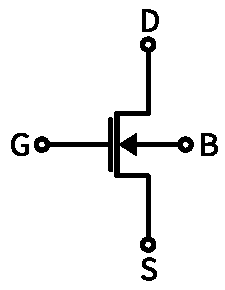
\includegraphics[keepaspectratio]{index_files/mediabag/index_files/figure-pdf/fig-nmos-symbol-output-1.pdf}}

}

\caption{\label{fig-nmos-symbol}Circuit symbol of n-channel MOSFET.}

\end{figure}%

\textsubscript{Source:
\href{https://iic-jku.github.io/analog-circuit-design/index.qmd.html}{Article
Notebook}}

\begin{figure}[H]

\centering{

\pandocbounded{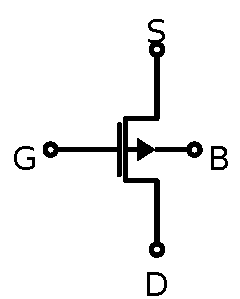
\includegraphics[keepaspectratio]{index_files/mediabag/index_files/figure-pdf/fig-pmos-symbol-output-1.pdf}}

}

\caption{\label{fig-pmos-symbol}Circuit symbol of p-channel MOSFET.}

\end{figure}%

\textsubscript{Source:
\href{https://iic-jku.github.io/analog-circuit-design/index.qmd.html}{Article
Notebook}}

For hand calculations and theoretical discussions we will use the
following simplified large-signal model, shown in
Figure~\ref{fig-mosfet-large-signal-model}. A current source
\(I_\mathrm{D}\) models the current flow between drain and source, and
it is controlled by the three control voltages \(V_\mathrm{GS}\),
\(V_\mathrm{DS}\), and \(V_\mathrm{SB}\). Note that in this way (since
\(I_\mathrm{D}= f(V_\mathrm{DS})\)) also a resistive behavior between D
and S can be modelled. In case that B and S are shorted then simply
\(V_\mathrm{SB} = 0\) and \(C_\mathrm{SB}\) is shorted.

\textsubscript{Source:
\href{https://iic-jku.github.io/analog-circuit-design/index.qmd.html}{Article
Notebook}}

\begin{figure}[H]

\centering{

\pandocbounded{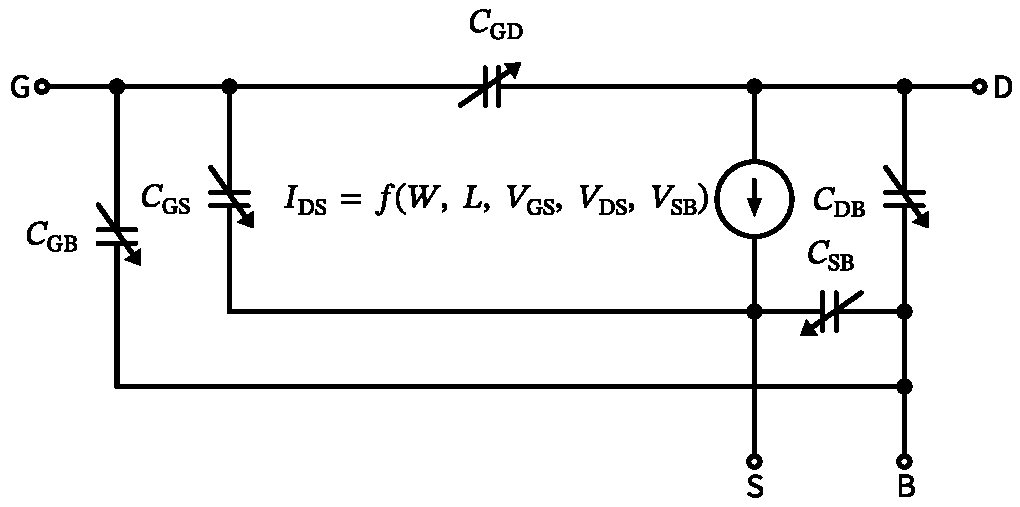
\includegraphics[keepaspectratio]{index_files/mediabag/index_files/figure-pdf/fig-mosfet-large-signal-model-output-1.pdf}}

}

\caption{\label{fig-mosfet-large-signal-model}The MOSFET large-signal
model. In general, all capacitors are nonlinear, i.e., they depend on
their terminal voltages.}

\end{figure}%

\textsubscript{Source:
\href{https://iic-jku.github.io/analog-circuit-design/index.qmd.html}{Article
Notebook}}

In an ideal MOSFET no dc current is flowing into the gate, the behavior
is purely capacitive. We model this by two capacitors:
\(C_\mathrm{GG}= C_\mathrm{GS}+ C_\mathrm{GD}+ C_\mathrm{GB}\) is the
total capacitance when looking into the gate of the MOSFET.
\(C_\mathrm{GS}\) is usually the dominant capacitance, and
\(C_\mathrm{GD}\) models the capacitive feedback between D and G,
usually induced by a topological overlap capacitance in the physical
construction of the MOSFET. This capacitance is often small compared to
\(C_\mathrm{GS}\), but in situations where we have a large voltage swing
at the drain this capacitance will be affected by the
\href{https://en.wikipedia.org/wiki/Miller_effect}{Miller effect} (see
Section~\ref{sec-miller-theorem}). In hand calculations we will often
set \(C_\mathrm{GD}= C_\mathrm{GB}= C_\mathrm{DB}= C_\mathrm{SB}= 0\).

To model a physical MOSFET there will be also a requirement for
resistors in the model to account for terminal access resistances
(\(R_\mathrm{G}\), \(R_\mathrm{D}\), and \(R_\mathrm{S}\)) as well as
resistors to model second-order effects like non-quasistatic operation.
For lower frequencies and bulk MOSFETs we will not consider these
resistors, and just deal with the capacitive behavior.

\begin{tcolorbox}[enhanced jigsaw, breakable, arc=.35mm, colbacktitle=quarto-callout-note-color!10!white, toprule=.15mm, left=2mm, toptitle=1mm, bottomtitle=1mm, opacityback=0, rightrule=.15mm, opacitybacktitle=0.6, titlerule=0mm, colback=white, colframe=quarto-callout-note-color-frame, coltitle=black, title=\textcolor{quarto-callout-note-color}{\faInfo}\hspace{0.5em}{MOSFET Bulk Terminal}, bottomrule=.15mm, leftrule=.75mm]

In many situations we will connect the bulk and source terminals of a
MOSFET together, which results in a simplified large-signal model. As an
exercise, look at Figure~\ref{fig-mosfet-large-signal-model} and draw
this simplified model (hint: look at
Figure~\ref{fig-mosfet-small-signal-model} and
Figure~\ref{fig-mosfet-small-signal-model-simplified} for inspiration).

\end{tcolorbox}

Now, as we are skipping the bottom-up approach of deriving the MOSFET
large-signal behavior from basic principles, we need to understand the
behavior of the elements of the large-signal model in
Figure~\ref{fig-mosfet-large-signal-model} by using a circuit simulator
and observing what happens. And generally, a first step in any new IC
technology should be to investigate basic MOSFET performance, by doing
simple dc sweeps of \(V_\mathrm{GS}\) and \(V_\mathrm{DS}\) and looking
at \(I_\mathrm{D}\) and other large- and small-signal parameters.

As a side note, the students who want to understand MOSFET behavior from
a physical angle should consult the MOSFET chapter from the JKU course
``Design of Complex Integrated Circuits'' (VL 336.048). A great
introduction into MOSFET operation and fabrication is given in (Hu
2010), which is available freely
\href{https://www.chu.berkeley.edu/modern-semiconductor-devices-for-integrated-circuits-chenming-calvin-hu-2010/}{online}
and is a recommended read. A very detailed description of the MOSFET
(leaving usually no question unanswered) is provided in (Tsividis and
McAndrew 2011).

Now, in order to get started, basic Xschem testbenches are prepared, and
first simple dc sweeps of various voltages and currents will be done.
But before that, please look at the import note below!

\begin{tcolorbox}[enhanced jigsaw, breakable, arc=.35mm, colbacktitle=quarto-callout-important-color!10!white, toprule=.15mm, left=2mm, toptitle=1mm, bottomtitle=1mm, opacityback=0, rightrule=.15mm, opacitybacktitle=0.6, titlerule=0mm, colback=white, colframe=quarto-callout-important-color-frame, coltitle=black, title=\textcolor{quarto-callout-important-color}{\faExclamation}\hspace{0.5em}{Mathematical Notation}, bottomrule=.15mm, leftrule=.75mm]

Throughout this material, we will largely stick to the following
notation standardized by IEEE:

\begin{itemize}
\tightlist
\item
  A \textbf{dc quantity} is shown with an upper-case variable name with
  upper-case subscripts, like \(V_\mathrm{GS}\).
\item
  Double-subscripts denote \textbf{dc sources}, like \(V_\mathrm{DD}\)
  and \(V_\mathrm{SS}\).
\item
  An \textbf{ac (small-signal) quantity} (incremental quantity) has a
  lower-case variable name with a lower-case subscript, like
  \(g_\mathrm{m}\).
\item
  A \textbf{total quantity} (dc plus ac) is shown as a lowercase
  variable name with upper-case subscript, like \(i_\mathrm{DS}\).
\item
  An upper-case variable name with a lower-case subscript is used to
  denote \textbf{RMS quantities}, like \(I_\mathrm{ds}\).
\end{itemize}

\end{tcolorbox}

\begin{tcolorbox}[enhanced jigsaw, breakable, arc=.35mm, colbacktitle=quarto-callout-note-color!10!white, toprule=.15mm, left=2mm, toptitle=1mm, bottomtitle=1mm, opacityback=0, rightrule=.15mm, opacitybacktitle=0.6, titlerule=0mm, colback=white, colframe=quarto-callout-note-color-frame, coltitle=black, title=\textcolor{quarto-callout-note-color}{\faInfo}\hspace{0.5em}{A Comment on Active and Passive Devices and Linear vs.~Nonlinear}, bottomrule=.15mm, leftrule=.75mm]

In contrast to the \textbf{passive} devices resistor \(R\), inductor
\(L\), and capacitor \(C\), which can only dissipate energy (and are
often treated in a linearized fashion), transistors (like the MOSFET)
are called ``\textbf{active}'', since they can provide signal power
amplification. However, transistors can not create energy out of thin
air, but merely convert \textbf{dc} energy (supplied by the power
supply) into \textbf{ac} energy. They have to have nonlinear transfer
characteristics to do this, but it has been shown that a
piecewise-linear characteristic is sufficient (Jakoby 2022). This is
very good news for circuit design, as usually we strive for linear
behaviour!

\end{tcolorbox}

\subsubsection{Large-Signal MOSFET
Model}\label{large-signal-mosfet-model}

We start with an investigation into the large-signal MOSFET model shown
in Figure~\ref{fig-mosfet-large-signal-model} by using the simple
testbench for the LV NMOS shown in Figure~\ref{fig-simple-nmos-tb}.

\begin{figure}

\centering{

\pandocbounded{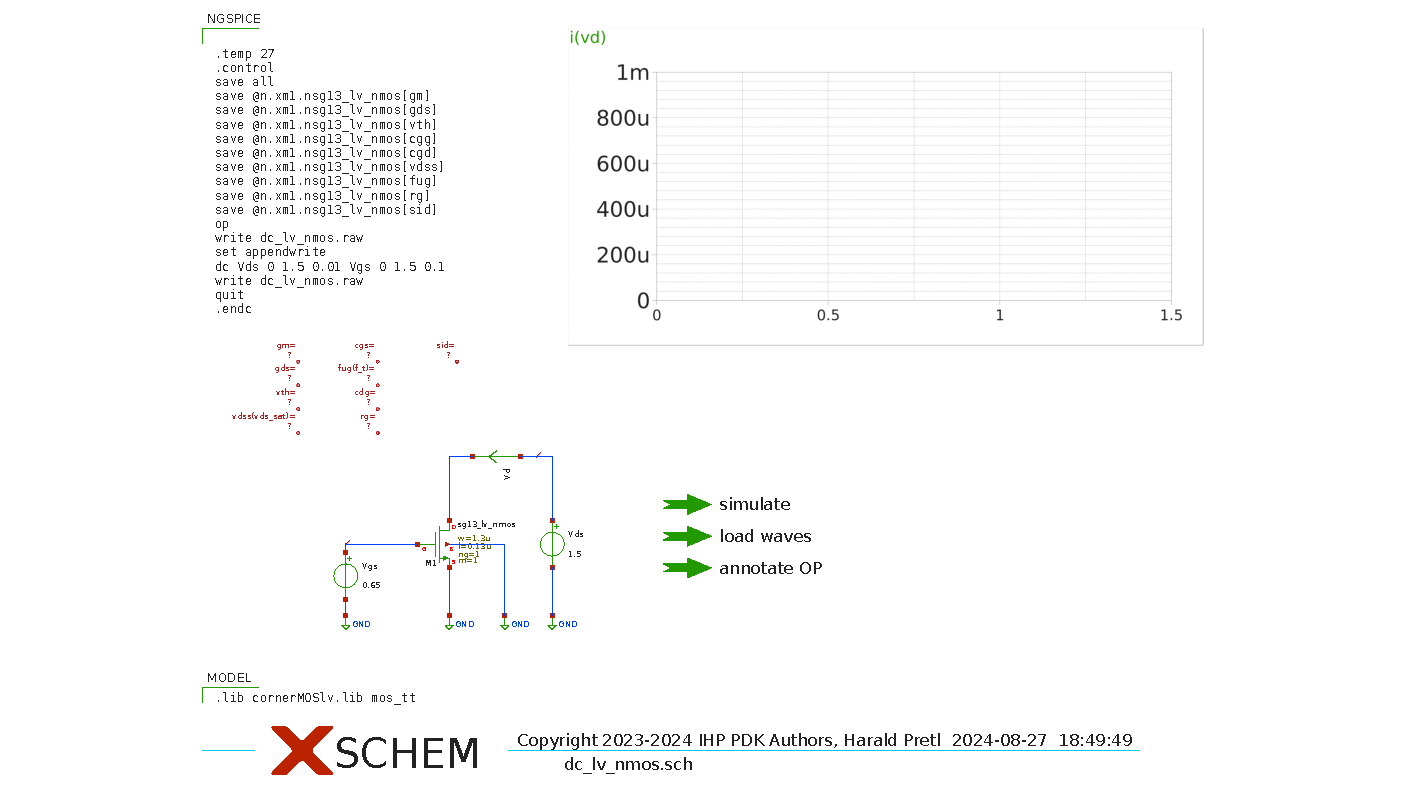
\includegraphics[keepaspectratio]{index_files/mediabag/xschem/dc_lv_nmos.pdf}}

}

\caption{\label{fig-simple-nmos-tb}Testbench for NMOS dc sweeps.}

\end{figure}%

\begin{tcolorbox}[enhanced jigsaw, breakable, arc=.35mm, colbacktitle=quarto-callout-note-color!10!white, toprule=.15mm, left=2mm, toptitle=1mm, bottomtitle=1mm, opacityback=0, rightrule=.15mm, opacitybacktitle=0.6, titlerule=0mm, colback=white, colframe=quarto-callout-note-color-frame, coltitle=black, title=\textcolor{quarto-callout-note-color}{\faInfo}\hspace{0.5em}{MOSFET Simulation Model}, bottomrule=.15mm, leftrule=.75mm]

For modelling the MOSFET behavior in a circuit simulator like ngspice
different models are available. Some of these models have been widely
adopted, like the \href{https://en.wikipedia.org/wiki/BSIM}{BSIM}
(Berkeley Short-channel IGFET Model) or PSP (Philips Penn State) model.
The PSP model version 103.6 is used in the IHP SG13G2 PDK for the LV and
HV MOSFET. This model has several advantages:

\begin{itemize}
\tightlist
\item
  Physics-based surface-potential model
\item
  Symmetric formulation with respect to drain and source
\item
  Support for mobility reduction, velocity saturation, DIBL, gate
  current, lateral doping gradient effects, STI stress, NQS, etc.
\end{itemize}

The PSP 103.6 model documentation can be found
\href{https://www.cea.fr/cea-tech/leti/pspsupport/Documents/psp103p6_summary.pdf}{here}.
In chapter 8 the dc operating point output of the model (these
parameters can be queried in ngspice) is explained, which is helpful to
interpret the simulation output.

\end{tcolorbox}

\begin{tcolorbox}[enhanced jigsaw, breakable, arc=.35mm, colbacktitle=quarto-callout-tip-color!10!white, toprule=.15mm, left=2mm, toptitle=1mm, bottomtitle=1mm, opacityback=0, rightrule=.15mm, opacitybacktitle=0.6, titlerule=0mm, colback=white, colframe=quarto-callout-tip-color-frame, coltitle=black, title=\textcolor{quarto-callout-tip-color}{\faLightbulb}\hspace{0.5em}{Exercise: MOSFET Investigation}, bottomrule=.15mm, leftrule=.75mm]

Please try to execute the following steps and answer these questions:

\begin{enumerate}
\def\labelenumi{\arabic{enumi}.}
\tightlist
\item
  Get the LV NMOS testbench (available at
  \url{https://github.com/iic-jku/analog-circuit-design/blob/main/xschem/dc_lv_nmos.sch})
  working in your IIC-OSIC-TOOLS environment.
\item
  Make yourself familiar with Xschem (change the schematic in various
  ways, run a simulation, graph the result).
\item
  Make yourself familiar with ngspice (run various simulations, save
  nets and parameters, use the embedded Xschem graphing, explore the
  interactive ngspice shell to look at MOSFET model parameters).
\item
  Explore the LV NMOS \texttt{sg13\_lv\_nmos}:

  \begin{enumerate}
  \def\labelenumii{\arabic{enumii}.}
  \tightlist
  \item
    How is \(I_\mathrm{D}\) affected by \(V_\mathrm{GS}\) and
    \(V_\mathrm{DS}\)?
  \item
    Change \(W\) and \(L\) of the MOSFET. What is the impact on the
    above parameters? Can you explain the variations?
  \item
    Look at the capacitance values for \(C_\mathrm{GS}\),
    \(C_\mathrm{GB}\), \(C_\mathrm{GD}\), and \(C_\mathrm{DB}\). How are
    they affected by \(W\) and \(L\) and by changing the bias conditions
    (play with \(V_\mathrm{GS}\) and \(V_\mathrm{DS}\))?
  \item
    When looking at the model parameters in ngspice, you see that there
    is a \(C_\mathrm{GD}\) and a \(C_\mathrm{DG}\). Why is this, what
    could be the difference? Sometimes these capacitors show a negative
    value, why? (Hint: Study Note~\ref{nte-maxwell-cap-matrix})
  \end{enumerate}
\item
  Build testbenches in Xschem for the LV PMOS, the HV NMOS, and the HV
  PMOS. Explore the different results.

  \begin{enumerate}
  \def\labelenumii{\arabic{enumii}.}
  \tightlist
  \item
    For a given \(W\) and \(L\), which device provides more drain
    current? How are the capacitances related?
  \item
    If you would have to size an inverter, what would be the ideal ratio
    of \(W_p/W_n\)? Will you exactly design this ratio, or are the
    reasons to deviate?
  \item
    There are LV and HV MOSFETs, and you investigated the difference in
    performance. What is the rationale when designing circuits for
    selection either an LV type, and when to choose an HV type?
  \end{enumerate}
\item
  Build a test bench to explore the body effect, start with LV NMOS.

  \begin{enumerate}
  \def\labelenumii{\arabic{enumii}.}
  \tightlist
  \item
    What happens when \(V_\mathrm{SB}\neq 0\)?
  \end{enumerate}
\end{enumerate}

\end{tcolorbox}

\subsubsection{Small-Signal MOSFET
Model}\label{sec-mosfet-smallsignal-model}

As you have seen in the previous investigations, the large-signal model
of Figure~\ref{fig-mosfet-large-signal-model} describes the behavior of
the MOSFET across a wide range of voltages applied at the MOSFET
terminals. Unfortunately, for hand analysis dealing with a nonlinear
model is close to impossible, at the very least it is quite tedious.

However, for many practical situations, we bias a MOSFET with a set of
dc voltages applied to its terminal, and only apply small signal
excursions during operation. If we do this, we can linearize the
large-signal model in this dc operating point, and resort to a
small-signal model which can be very useful for hand calculations. Many
experienced designers analyze their circuits by doing these kind of hand
calculations and describing the circuit analytically, which is a great
way to understand fundamental performance limits and relationships
between parameters.

We will use the small-signal MOSFET model shown in
Figure~\ref{fig-mosfet-small-signal-model} for this course. The
current-source \(i_\mathrm{d}= g_\mathrm{m}v_\mathrm{gs}\) models the
drain current \(I_\mathrm{D}\) as a function of \(V_\mathrm{GS}\) with

\[
g_\mathrm{m}= \frac{\partial I_\mathrm{D}(V_\mathrm{GS}, V_\mathrm{DS}, V_\mathrm{SB})}{\partial V_\mathrm{GS}},
\]

and the resistor \(g_\mathrm{ds}\) models the dependency of the drain
current by \(V_\mathrm{DS}\):

\[
g_\mathrm{ds}= \frac{\partial I_\mathrm{D}(V_\mathrm{GS}, V_\mathrm{DS}, V_\mathrm{SB})}{\partial V_\mathrm{DS}}
\]

The drain current dependency on the source-bulk voltage (the so-called
``body effect'') is introduced by the current source
\(i_\mathrm{d}= g_\mathrm{mb} v_\mathrm{sb}\):

\[
g_\mathrm{mb}= \frac{\partial I_\mathrm{D}(V_\mathrm{GS}, V_\mathrm{DS}, V_\mathrm{SB})}{\partial V_\mathrm{SB}}
\]

\textsubscript{Source:
\href{https://iic-jku.github.io/analog-circuit-design/index.qmd.html}{Article
Notebook}}

\begin{figure}[H]

\centering{

\pandocbounded{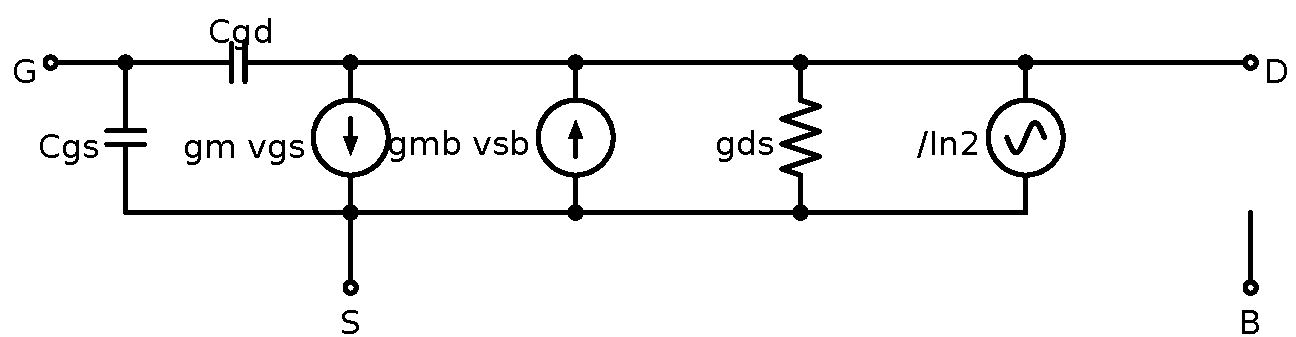
\includegraphics[keepaspectratio]{index_files/mediabag/index_files/figure-pdf/fig-mosfet-small-signal-model-output-1.pdf}}

}

\caption{\label{fig-mosfet-small-signal-model}The MOSFET small-signal
model.}

\end{figure}%

\textsubscript{Source:
\href{https://iic-jku.github.io/analog-circuit-design/index.qmd.html}{Article
Notebook}}

As has been mentioned before, in many situations (and whenever we want
to use a simplified model) we connect source and bulk of the MOSFET
together. This results in the much simplified small-signal model shown
in Figure~\ref{fig-mosfet-small-signal-model-simplified}.

\textsubscript{Source:
\href{https://iic-jku.github.io/analog-circuit-design/index.qmd.html}{Article
Notebook}}

\begin{figure}[H]

\centering{

\pandocbounded{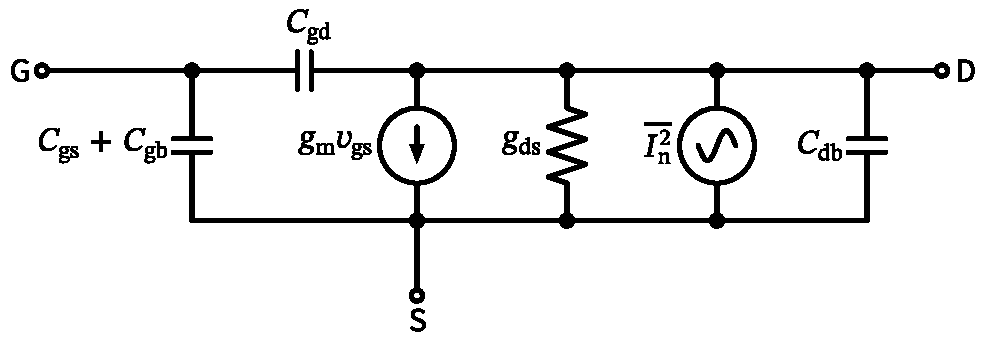
\includegraphics[keepaspectratio]{index_files/mediabag/index_files/figure-pdf/fig-mosfet-small-signal-model-simplified-output-1.pdf}}

}

\caption{\label{fig-mosfet-small-signal-model-simplified}The MOSFET
small-signal model when source and bulk are shorted.}

\end{figure}%

\textsubscript{Source:
\href{https://iic-jku.github.io/analog-circuit-design/index.qmd.html}{Article
Notebook}}

As any electronic device the MOSFET introduces noise into the circuit.
In this course we will only consider the \textbf{drain-source current
noise} of the MOSFET, given by

\begin{equation}\phantomsection\label{eq-mosfet-noise}{
\overline{I_\mathrm{n}^2} = 4 k T \gamma g_\mathrm{d0},
}\end{equation}

where \(\overline{I_\mathrm{n}^2}\) is the one-sided power-spectral
density of the noise in A\(^2\)/Hz; \(k\) is the Boltzmann constant;
\(T\) is the absolute temperature; \(\gamma\) is a (fitting) parameter
in simplified theory changing between \(\gamma = 2/3\) in saturation and
\(\gamma =1\) for triode operation; \(g_\mathrm{d0}\) is equal to
\(g_\mathrm{m}\) in saturation and \(g_\mathrm{ds}\) in triode).

\begin{tcolorbox}[enhanced jigsaw, breakable, arc=.35mm, colbacktitle=quarto-callout-note-color!10!white, toprule=.15mm, left=2mm, toptitle=1mm, bottomtitle=1mm, opacityback=0, rightrule=.15mm, opacitybacktitle=0.6, titlerule=0mm, colback=white, colframe=quarto-callout-note-color-frame, coltitle=black, title=\textcolor{quarto-callout-note-color}{\faInfo}\hspace{0.5em}{MOSFET Triode and Saturation Region}, bottomrule=.15mm, leftrule=.75mm]

Sometimes we will refer to different operating modes of the MOSFET like
``saturation'' or ``triode.'' Generally speaking, when the drain-source
voltage is small, then the MOSFET acts as a voltage-controlled resistor
(since the impact of both \(V_\mathrm{GS}\) and \(V_\mathrm{DS}\) on
\(I_\mathrm{D}\) is large), and this mode of operation we call
``\textbf{triode}'' mode.

When the drain-source voltage \(V_\mathrm{DS}\) is increased, at some
point the drain-source current saturates and is only a weak function of
the drain-source voltage, while still being well controlled by
\(V_\mathrm{GS}\). This mode is called ``\textbf{saturation}'' mode.

As you can see in the large-signal investigations, these transitions
happen gradually, and it is difficult to define a precise point where
one operating mode switches to the other one. In this sense we use terms
like ``triode'' and ``saturation'' only in an approximate sense.

\end{tcolorbox}

We can also consider an even more reduced small-signal MOSFET model
compared to Figure~\ref{fig-mosfet-small-signal-model-simplified}, which
is shown in Figure~\ref{fig-mosfet-small-signal-model-basic}. In this,
we just consider the transconductance \(g_\mathrm{m}\), the input
capacitor \(C_\mathrm{gg}\), as well as the output conductance
\(g_\mathrm{ds}\). Note that we can redraw the pi-model of
Figure~\ref{fig-mosfet-small-signal-model-basic} into the \(\tau\)-model
of Figure~\ref{fig-mosfet-small-signal-model-basic-t}. Depending on the
circuit configuration, either the first or the second form results in
simpler calculations of the circuit equations.

\textsubscript{Source:
\href{https://iic-jku.github.io/analog-circuit-design/index.qmd.html}{Article
Notebook}}

\begin{figure}[H]

\centering{

\pandocbounded{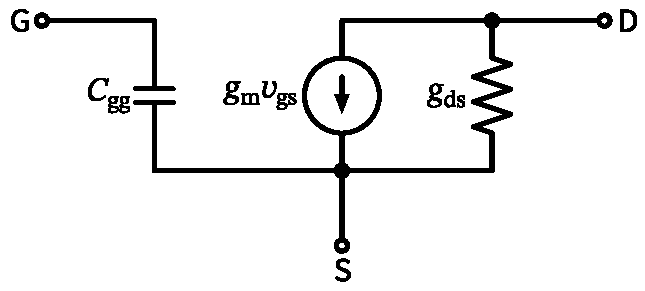
\includegraphics[keepaspectratio]{index_files/mediabag/index_files/figure-pdf/fig-mosfet-small-signal-model-basic-output-1.pdf}}

}

\caption{\label{fig-mosfet-small-signal-model-basic}The MOSFET
small-signal basic pi-model.}

\end{figure}%

\textsubscript{Source:
\href{https://iic-jku.github.io/analog-circuit-design/index.qmd.html}{Article
Notebook}}

\begin{figure}[H]

\centering{

\pandocbounded{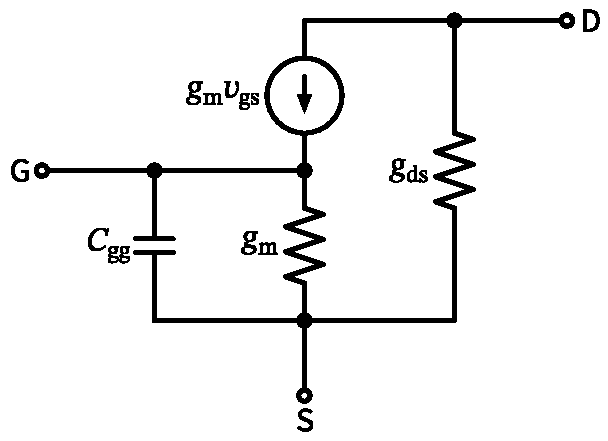
\includegraphics[keepaspectratio]{index_files/mediabag/index_files/figure-pdf/fig-mosfet-small-signal-model-basic-t-output-1.pdf}}

}

\caption{\label{fig-mosfet-small-signal-model-basic-t}The MOSFET
small-signal basic T-model.}

\end{figure}%

\textsubscript{Source:
\href{https://iic-jku.github.io/analog-circuit-design/index.qmd.html}{Article
Notebook}}

\begin{tcolorbox}[enhanced jigsaw, breakable, arc=.35mm, colbacktitle=quarto-callout-tip-color!10!white, toprule=.15mm, left=2mm, toptitle=1mm, bottomtitle=1mm, opacityback=0, rightrule=.15mm, opacitybacktitle=0.6, titlerule=0mm, colback=white, colframe=quarto-callout-tip-color-frame, coltitle=black, title=\textcolor{quarto-callout-tip-color}{\faLightbulb}\hspace{0.5em}{Exercise: MOSFET Model Transformation}, bottomrule=.15mm, leftrule=.75mm]

Can you show, with which circuit manipulations you can transform the
pi-model of Figure~\ref{fig-mosfet-small-signal-model-basic} into the
T-model of Figure~\ref{fig-mosfet-small-signal-model-basic-t}?

\end{tcolorbox}

A metric which is useful to assess the speed of a MOSFET is the
so-called \textbf{transit frequency} \(f_\mathrm{T}\). It is defined as
the frequency where the small-signal current gain (output current
divided by the input current) of a MOSFET driven by a voltage-source at
the input and loaded by a voltage source at the output drops to unity
(reaches one). It can easily be derived using the simplified MOSFET
small-signal model of
Figure~\ref{fig-mosfet-small-signal-model-simplified} by driving it with
a voltage source and shorting the output to (neglecting the feed-forward
current introduced by \(C_\mathrm{gd}\))
\begin{equation}\phantomsection\label{eq-mosfet-transit-frequency}{
\omega_\mathrm{T} = 2 \pi f_\mathrm{T} \approx \frac{g_\mathrm{m}}{C_\mathrm{gg}} = \frac{g_\mathrm{m}}{C_\mathrm{gs}+ C_\mathrm{gd}+ C_\mathrm{gb}}.
}\end{equation} This frequency is an extrapolated frequency where the
MOSFET operation is dominated by several second-order effects (hence
Equation~\ref{eq-mosfet-transit-frequency} is not valid any longer). A
rule-of-thumb is to use a MOSFET up to approximately
\(f_\mathrm{T} / 10\). In any case, \(f_\mathrm{T}\) is a proxy of the
speed of a MOSFET; in other words, how much input capacitance
\(C_\mathrm{gg}\) is incurred when creating a certain \(g_\mathrm{m}\).

\begin{tcolorbox}[enhanced jigsaw, breakable, arc=.35mm, colbacktitle=quarto-callout-tip-color!10!white, toprule=.15mm, left=2mm, toptitle=1mm, bottomtitle=1mm, opacityback=0, rightrule=.15mm, opacitybacktitle=0.6, titlerule=0mm, colback=white, colframe=quarto-callout-tip-color-frame, coltitle=black, title=\textcolor{quarto-callout-tip-color}{\faLightbulb}\hspace{0.5em}{Exercise: MOSFET Transit Frequency}, bottomrule=.15mm, leftrule=.75mm]

As a home exercise, try to derive
Equation~\ref{eq-mosfet-transit-frequency} starting from
Figure~\ref{fig-mosfet-small-signal-model-simplified}. By showing this
transformation you can proof that indeed both circuits are electrically
equivalent.

\end{tcolorbox}

Now we need to see how the small-signal parameters seen in
Figure~\ref{fig-mosfet-small-signal-model} can be investigated and
estimated using circuit simulation.

\begin{tcolorbox}[enhanced jigsaw, breakable, arc=.35mm, colbacktitle=quarto-callout-tip-color!10!white, toprule=.15mm, left=2mm, toptitle=1mm, bottomtitle=1mm, opacityback=0, rightrule=.15mm, opacitybacktitle=0.6, titlerule=0mm, colback=white, colframe=quarto-callout-tip-color-frame, coltitle=black, title=\textcolor{quarto-callout-tip-color}{\faLightbulb}\hspace{0.5em}{Exercise: MOSFET Small-Signal Parameters}, bottomrule=.15mm, leftrule=.75mm]

Please try to execute the following steps and answer the following
questions:

\begin{enumerate}
\def\labelenumi{\arabic{enumi}.}
\tightlist
\item
  Reuse the LV NMOS testbench (available at
  \url{https://github.com/iic-jku/analog-circuit-design/blob/main/xschem/dc_lv_nmos.sch}).
\item
  Explore the LV NMOS \texttt{sg13\_lv\_nmos}:

  \begin{enumerate}
  \def\labelenumii{\arabic{enumii}.}
  \tightlist
  \item
    How are \(g_\mathrm{m}\) and \(g_\mathrm{ds}\) changing when you
    change the dc node voltages?
  \item
    What is the ratio of \(g_\mathrm{m}\) to \(g_\mathrm{mb}\)? What is
    the physical reason behind this ratio (you might want to revisit
    MOSFET device physics at this point)?
  \item
    Take a look at the device capacitances \(C_\mathrm{gs}\),
    \(C_\mathrm{gd}\), and \(C_\mathrm{gb}\). Why are they important?
    What is the \(f_\mathrm{T}\) of the MOSFET?
  \item
    Look at the drain noise current according to the MOSFET model and
    compare with a hand calculation of the noise. In the noise equation
    there is the factor \(\gamma\), which in triode is \(\gamma=1\) and
    in saturation is \(\gamma=2/3\) according to basic text books. Which
    value of \(\gamma\) are you calculating? Why might it be different?
  \end{enumerate}
\item
  Go back to your testbench for the LVS PMOS \texttt{sg13\_lv\_pmos}:

  \begin{enumerate}
  \def\labelenumii{\arabic{enumii}.}
  \tightlist
  \item
    What is the difference in \(g_\mathrm{m}\), \(g_\mathrm{ds}\), and
    other parameters between the NMOS and the PMOS? Why could they be
    different?
  \end{enumerate}
\end{enumerate}

\end{tcolorbox}

\begin{tcolorbox}[enhanced jigsaw, breakable, arc=.35mm, colbacktitle=quarto-callout-note-color!10!white, toprule=.15mm, left=2mm, toptitle=1mm, bottomtitle=1mm, opacityback=0, rightrule=.15mm, opacitybacktitle=0.6, titlerule=0mm, colback=white, colframe=quarto-callout-note-color-frame, coltitle=black, title=\textcolor{quarto-callout-note-color}{\faInfo}\hspace{0.5em}{Note \ref*{nte-maxwell-cap-matrix}: Maxwell Capacitance Matrix}, bottomrule=.15mm, leftrule=.75mm]

\quartocalloutnte{nte-maxwell-cap-matrix} 

A Maxwell capacitance matrix (Maxwell 1873) provides the relation
between voltages on a set of conductors and the charges on these
conductors. For a given conductor set with \(N\) conductors (and thus
\(N\) terminals) the relation is \[
\mathbf{Q} = \mathbf{C} \cdot \mathbf{V}
\] where \(\mathbf{Q}\) is a vector of the charges on the \(N\)
conductors, \(\mathbf{C}\) is a \(N \times N\) capacitance matrix, and
\(\mathbf{V}\) is the potential vector. In the case of two conductors
and physical capacitances between them, \(\mathbf{C}\) is given by \[
\mathbf{C} =
\begin{pmatrix}
C_{11} + C_{12} & -C_{12} \\
-C_{21} & C_{21} + C_{22} \\
\end{pmatrix}
\] where \(C_{xx} = \partial Q_x / \partial V_x\) is the auto
capacitance from a conductor \(x\) towards infinity (ground), and
\(C_{xy} = \partial Q_x / \partial V_y\) is the mutual capacitance from
node/conductor \(x\) to node/conductor \(y\). For a physical capacitor
\(C_{xy} = C_{yx}\).

Using the above equation to calculate \(Q_1\) (the charge on conductor
\(1\)) results in \[
Q_1 = ( C_{11} + C_{12} ) V_1 - C_{12} V_2 = C_{11} (V_1 - 0) + C_{12} (V_1 - V_2)
\] which is the expected result.

Such a Maxwell capacitance formulation is also used in the MOSFET model
to describe the charge at a terminal as a function of potential at
another terminal. So, \[
C_\mathrm{GD}= \frac{\partial Q_\mathrm{G}}{\partial V_\mathrm{D}}
\] or \[
C_\mathrm{GG}= \frac{\partial Q_\mathrm{G}}{\partial V_\mathrm{G}}
\] with \(Q_\mathrm{G}\) the charge at terminal G in response to either
\(V_\mathrm{D}\) or \(V_\mathrm{G}\). Note that in a MOSFET, generally
\(C_{xy} \ne C_{yx}\)!

\end{tcolorbox}

\subsection{Conclusion}\label{conclusion}

Congratulations for making it thus far! By now you should have a solid
grasp of the tool handling of Xschem and ngspice, and you should be
familiar with the large- and small-signal operation of both NMOS and
PMOS, and the parameters describing these behaviors. If you feel you are
not sufficiently fluent in these things, please go back to the beginning
of Section~\ref{sec-mosfet} and revisit the relevant sections, or dive
into further reading about the MOSFET operation, like in (Hu 2010).

\section{Transistor Sizing Using gm/ID
Methodology}\label{sec-gmid-method}

When designing integrated circuits it is an important question how to
select various parameters of a MOSFET, like \(W\), \(L\), or the bias
current \(I_\mathrm{D}\). In comparison to using discrete components in
PCB design, or also compared to a bipolar junction transistor (BJT), we
have these degrees of freedom, which make integrated circuit design so
interesting.

Often, transistor sizing in entry-level courses is based on the
square-law model, where a simple analytical equation for the drain
current can be derived. However, in nanometer CMOS, the MOSFET behavior
is much more complex than these simple models. Also, this highly
simplified derivations introduce concepts like the threshold voltage or
the overdrive voltage, which are interesting from a theoretical
viewpoint, but bear little practical use.

\begin{tcolorbox}[enhanced jigsaw, breakable, arc=.35mm, colbacktitle=quarto-callout-note-color!10!white, toprule=.15mm, left=2mm, toptitle=1mm, bottomtitle=1mm, opacityback=0, rightrule=.15mm, opacitybacktitle=0.6, titlerule=0mm, colback=white, colframe=quarto-callout-note-color-frame, coltitle=black, title=\textcolor{quarto-callout-note-color}{\faInfo}\hspace{0.5em}{MOSFET Square-Law Model}, bottomrule=.15mm, leftrule=.75mm]

One of the many simplifications of the square-law model is that the
mobility of the charge carriers is assumed constant (it is not).
Further, the existence of a threshold voltage is assumed, but in fact
this voltage is just existing given a certain definition, and depending
on definition, its value changed. In addition, in nm CMOS, the threshold
voltage is a function on many thing, like \(W\) and \(L\).

\end{tcolorbox}

An additional shortcoming of the square-law model is that it is only
valid in strong inversion, i.e.~for large \(V_\mathrm{GS}\) where the
drain current is dominated by the drift current. As soon as the
gate-source voltage gets smaller, the square-law model breaks, as the
drain current component based on diffusion currents gets dominant.
Modern compact MOSFET models (like the PSP model used in SG13G2) use
hundreds of parameters and fairly complex equations to somewhat properly
describe MOSFET behavior over a wide range of parameters like \(W\),
\(L\), and temperature. A modern approach to MOSFET sizing is thus based
on the thought to use exactly these MOSFET models, characterize them,
put the resulting data into tables and charts, and thus learn about the
complex MOSFET behavior and use it for MOSFET sizing.

Being a well-established approach we select the
\(g_\mathrm{m}/I_\mathrm{D}\) methodology introduced by P. Jespers and
B. Murmann in (Jespers and Murmann 2017). A brief introduction is
available
\href{https://github.com/iic-jku/analog-circuit-design/blob/main/sizing/Ref_Murmann_gmID.pdf}{here}
as well.

The \(g_\mathrm{m}/I_\mathrm{D}\) methodology has the huge advantage
that it catches MOSFET behavior quite accurately over a wide range of
operating conditions, and the curves look very similar for pretty much
all CMOS technologies, from micrometer bulk CMOS down to nanometer
FinFET devices. Of course the absolute values change, but the method
applies universally.

\subsection{MOSFET Characterization
Testbench}\label{sec-techsweep-testbench}

In order to get the required tabulated data we use a testbench in Xschem
which sweeps the terminal voltages, and records various large- and
small-signal parameters, which are then stored in large tables. The
testbench for the LV NMOS is shown in
Figure~\ref{fig-techsweep-nmos-tb}, and the TB for the LV PMOS is shown
in Figure~\ref{fig-techsweep-pmos-tb}.

\begin{tcolorbox}[enhanced jigsaw, breakable, arc=.35mm, colbacktitle=quarto-callout-note-color!10!white, toprule=.15mm, left=2mm, toptitle=1mm, bottomtitle=1mm, opacityback=0, rightrule=.15mm, opacitybacktitle=0.6, titlerule=0mm, colback=white, colframe=quarto-callout-note-color-frame, coltitle=black, title=\textcolor{quarto-callout-note-color}{\faInfo}\hspace{0.5em}{Note on Characterization Testbench}, bottomrule=.15mm, leftrule=.75mm]

The testbenches are relatively straightforward, with one exception: The
drain current noise is sensed via the drain voltage source \texttt{vd}
and converted to a noise voltage (node \texttt{n}) using a
current-controlled voltage source (CCVS). This is necessary as the
\texttt{.noise} simulation statement works with voltages.

\end{tcolorbox}

\begin{figure}

\centering{

\pandocbounded{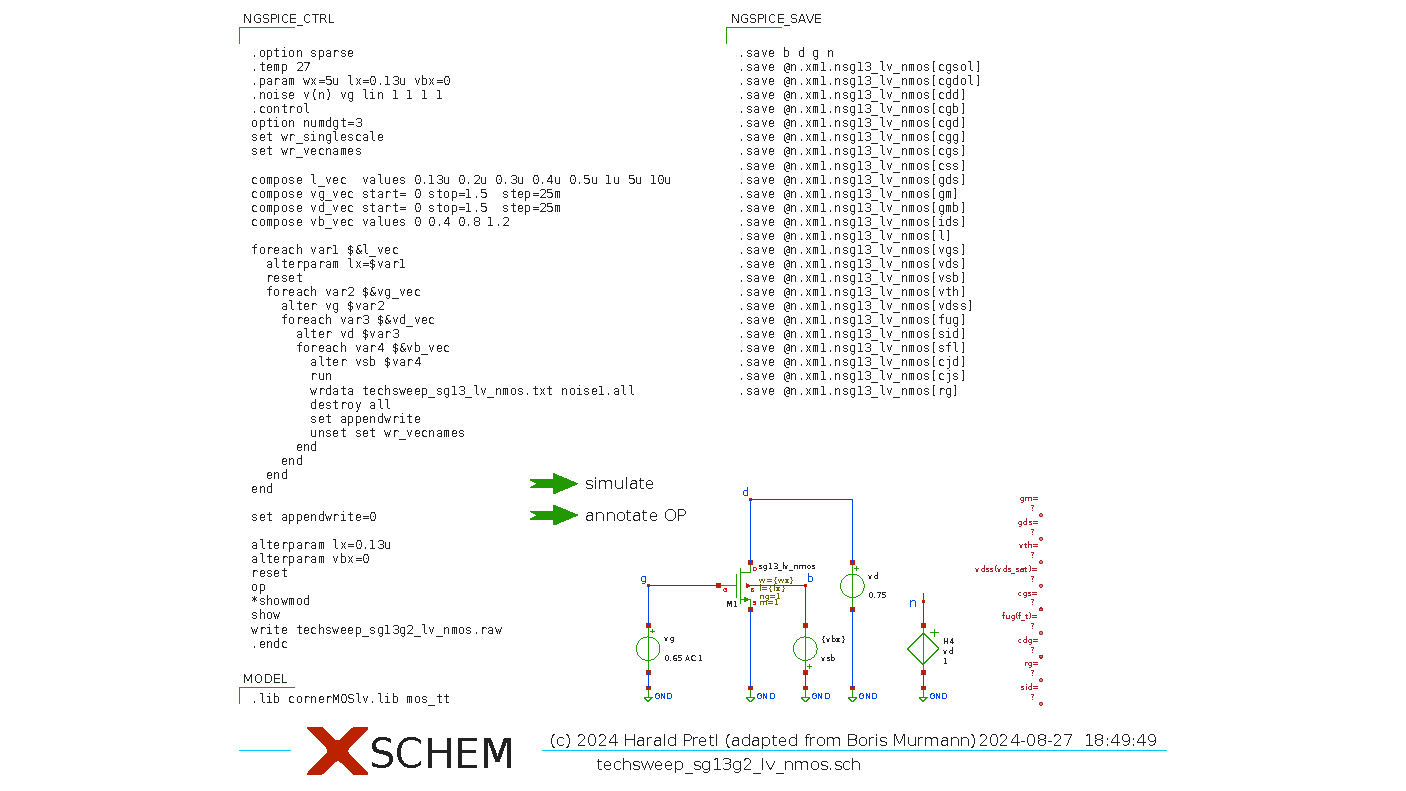
\includegraphics[keepaspectratio]{index_files/mediabag/xschem/techsweep_sg13g2_lv_nmos.pdf}}

}

\caption{\label{fig-techsweep-nmos-tb}Testbench for LV NMOS
\(g_\mathrm{m}/I_\mathrm{D}\) characterization.}

\end{figure}%

\begin{figure}

\centering{

\pandocbounded{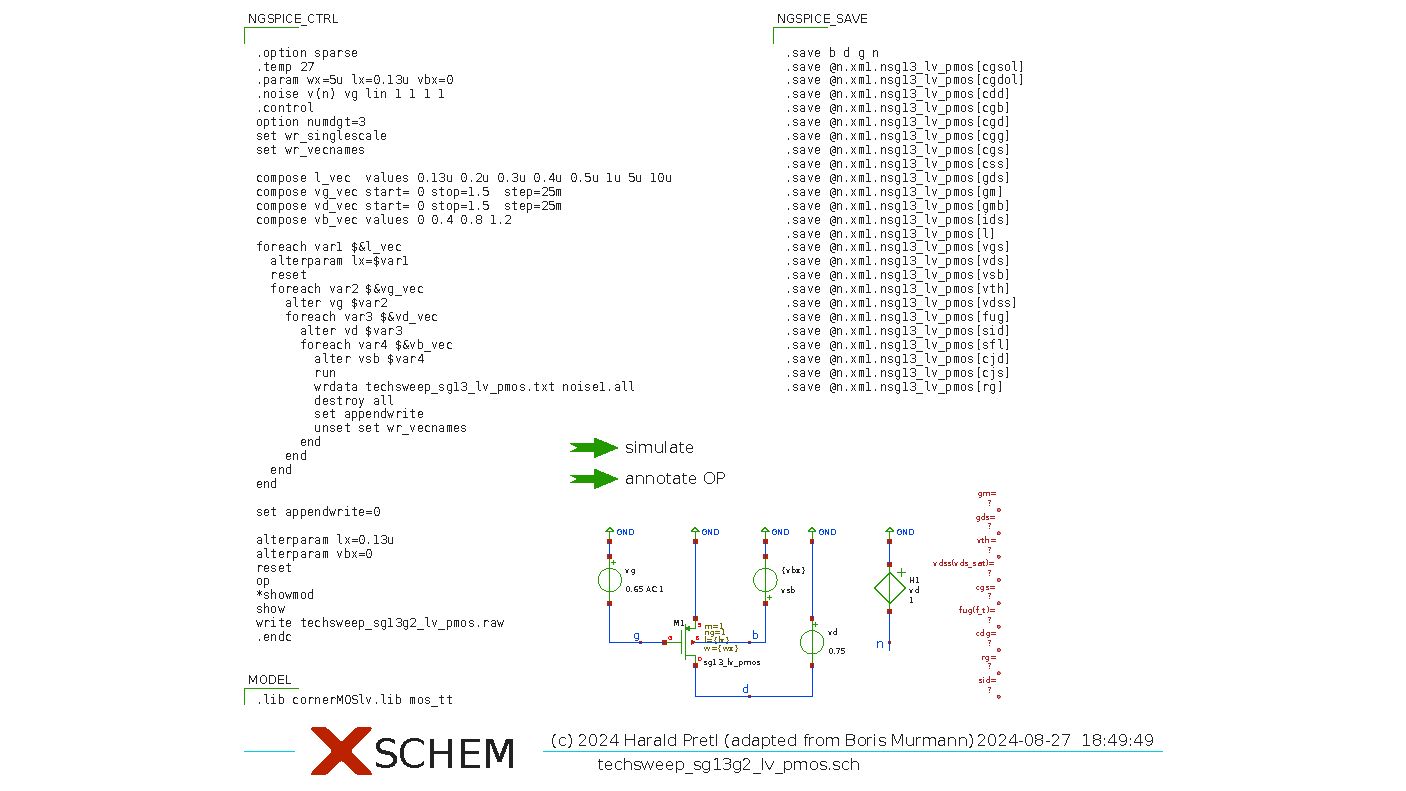
\includegraphics[keepaspectratio]{index_files/mediabag/xschem/techsweep_sg13g2_lv_pmos.pdf}}

}

\caption{\label{fig-techsweep-pmos-tb}Testbench for LV PMOS
\(g_\mathrm{m}/I_\mathrm{D}\) characterization.}

\end{figure}%

We will use Jupyter notebooks to inspect the resulting data, and
interpret some important graphs. This will greatly help to understand
the MOSFET behavior.

\subsection{NMOS Characterization in
Saturation}\label{sec-techsweep-nmos}

First, we will start looking at the LV NMOS. In
Section~\ref{sec-techsweep-pmos} we have the corresponding graphs for
the LV PMOS. In this lecture, we will only use the LV MOSFETs. While
there are also the HV types available, they are mainly used for
high-voltage circuits, like circuits connecting to the outside world.
Here, we only will design low-voltage circuits running at a nominal
supply voltage of \(1.5\,\text{V}\), so only the LV types are of
interest to us.

In the plots that follow we will set \(V_\mathrm{ds}= V_\mathrm{DD}/2\)
to keep the MOSFET in saturation (as this is the region of operation
where most MOSFET are operated when working in class-A). We will later
also look at the MOSFET performance in triode operation, as this is the
operation mode where the MOSFET is used as a switch. While the
\(g_\mathrm{m}/I_\mathrm{D}\) method is primarily intended to be used
for circuits where the MOSFETs are held in saturation and are biased by
a certain bias current (usually referred to
\href{https://en.wikipedia.org/wiki/Power_amplifier_classes\#Class_A}{class-A}),
the generated tables using the testbenches of
Section~\ref{sec-techsweep-testbench} contain the data for all MOSFET
bias points.

The first import graph is the plot of \(g_\mathrm{m}/I_\mathrm{D}\) and
\(f_\mathrm{T}\) versus the gate-source voltage \(V_\mathrm{GS}\). First
let us answer the question why \(g_\mathrm{m}/I_\mathrm{D}\) is a good
parameter to look at, and actually this is also the central parameter in
the \(g_\mathrm{m}/I_\mathrm{D}\) methodology. In many circuits we want
to get a large amplification from a MOSFET, which corresponds to a large
\(g_\mathrm{m}\). We want to achieve this by spending the minimum
biasing current possible (ideally zero), as we almost always design for
lowest power consumption. Thus, a high \(g_\mathrm{m}/I_\mathrm{D}\)
ratio is good.

\begin{tcolorbox}[enhanced jigsaw, breakable, arc=.35mm, colbacktitle=quarto-callout-note-color!10!white, toprule=.15mm, left=2mm, toptitle=1mm, bottomtitle=1mm, opacityback=0, rightrule=.15mm, opacitybacktitle=0.6, titlerule=0mm, colback=white, colframe=quarto-callout-note-color-frame, coltitle=black, title=\textcolor{quarto-callout-note-color}{\faInfo}\hspace{0.5em}{Power Consumption}, bottomrule=.15mm, leftrule=.75mm]

Designing for minimum power consumption is pretty much always mandated.
For battery-operated equipment it is a paramount requirement, but also
in other equipment electrical energy consumption is a concern, and often
severely limited by the cooling capabilities of the electrical system.

\end{tcolorbox}

However, as can be seen in the below plot, there exists a strong and
unfortunate trade-off with device speed, characterized here by the
transit frequency \(f_\mathrm{T}\). It would be ideal if there exists a
design point where we get high transconductance per bias current
concurrently to having the fastest operation, but unfortunately, this is
clearly not the case. The \(g_\mathrm{m}/I_\mathrm{D}\) peaks for
\(V_\mathrm{GS}< 0.3\,\text{V}\), and the highest speed we get at
\(V_\mathrm{GS}\approx 1.2\,\text{V}\). The dashed vertical line plots
the nominal threshold voltage, as you can see in this continuum of
parameter space, it marks not a particularly special point.

Note that
\begin{equation}\phantomsection\label{eq-mosfet-gmid-weakinversion}{
\frac{g_\mathrm{m}}{I_\mathrm{D}} = \frac{1}{n V_\mathrm{T}}
}\end{equation} for a MOSFET in weak inversion (i.e., small gate-source
voltage). \(n\) is the subthreshold slope, and
\(V_\mathrm{T} = k T / q\) which is \(25.8\,\text{mV}\) at
\(300\,\text{K}\). We thus have \(n \approx 1.38\) for this LV NMOS,
which falls nicely into the usual range for \(n\) of \(1.3\) to \(1.5\)
for bulk CMOS (FinFET have \(n\) very close to \(1\)).

For the classical square-law model of the MOSFET in strong inversion,
\(g_\mathrm{m}/I_\mathrm{D}\) is given as
\begin{equation}\phantomsection\label{eq-mosfet-gmid-stronginversion}{
\frac{g_\mathrm{m}}{I_\mathrm{D}} = \frac{2}{V_\mathrm{GS}- V_\mathrm{th}} = \frac{2}{V_\mathrm{od}} 
}\end{equation} with \(V_\mathrm{th}\) the threshold voltage and
\(V_\mathrm{od}\) the so-called ``overdrive voltage.'' The latter is
sometimes also dubbed the effective gate-source voltage
\(V_\mathrm{eff}\) (Carusone, Johns, and Martin 2011).

\begin{tcolorbox}[enhanced jigsaw, breakable, arc=.35mm, colbacktitle=quarto-callout-note-color!10!white, toprule=.15mm, left=2mm, toptitle=1mm, bottomtitle=1mm, opacityback=0, rightrule=.15mm, opacitybacktitle=0.6, titlerule=0mm, colback=white, colframe=quarto-callout-note-color-frame, coltitle=black, title=\textcolor{quarto-callout-note-color}{\faInfo}\hspace{0.5em}{Why 300K?}, bottomrule=.15mm, leftrule=.75mm]

Why are we so often using a temperature of \(300\,\text{K}\) for a
typical condition? As this corresponds to roughly
\(27^{\circ}\text{C}\), this accounts for some self heating compared to
otherwise cooler usual room temperatures. Further, engineers like round
numbers which are easy to remember, so \(300\,\text{K}\) is used as a
proxy for room temperature.

\end{tcolorbox}

As we can also see from belows plot, the peak transit frequency of the
LV NMOS is about \(75\,\text{GHz}\), which allows building
radio-frequency circuits up to ca.
\(f_\mathrm{T} / 10 = 7.5\,\text{GHz}\), which is a respectable number.
It is no coincidence, that the transition for RF design in the GHz-range
switched from BJT-based technologies to CMOS roughly in the time frame
when 130nm CMOS became available (ca. 2000).

Note that \(f_\mathrm{T}\) saturates and even decreases again at around
\(V_\mathrm{GS}= 1.2\,\text{V}\) due to second-order effects of the
transistor like
\href{https://en.wikipedia.org/wiki/Saturation_velocity}{velocity
saturation} and
\href{https://en.wikipedia.org/wiki/Drain-induced_barrier_lowering}{DIBL}.
Velocity saturation describes the saturation of the velocity of the
electrons at a certain \(V_\mathrm{GS}\). As a consequence, also
\(g_\mathrm{m}\) saturates. Since
\(f_\mathrm{T} \propto g_\mathrm{m}/ C_\mathrm{gs}\), \(f_\mathrm{T}\)
can not further increase. DIBL explains the effect when a too high
\(V_\mathrm{GS}\) is applied and therefore the channel is confined to a
narrow region at the surface, leading to more carrier scattering and
thus lower mobility.

\pandocbounded{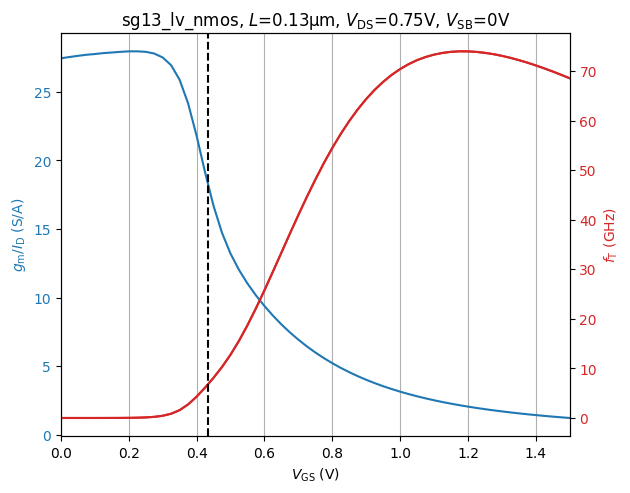
\includegraphics[keepaspectratio]{index_files/figure-latex/.-sizing-techsweep_sg13_plots_nmos-cell-6-output-1.png}}

\textsubscript{Source:
\href{https://iic-jku.github.io/analog-circuit-design/index.qmd.html}{Article
Notebook}}

The following figure plots \(f_\mathrm{T}\) against
\(g_\mathrm{m}/I_\mathrm{D}\) for several different \(L\). As you can
see, device speed maximizes for a low \(g_\mathrm{m}/I_\mathrm{D}\) and
a short \(L\). Note, that the drain-source voltage is kept at
\(V_\mathrm{DS}= 0.75\,\text{V} = V_\mathrm{DD}/ 2\), which is a typical
value keeping the MOSFET in saturation across the characterization
sweeps. Further, the source-bulk voltage is kept at
\(V_\mathrm{SB}= V_\mathrm{S} - V_\mathrm{B} = 0\,\text{V}\), which
means bulk and source terminals are connected. If
\(V_\mathrm{SB}\neq 0\,\text{V}\), then the so-called
\href{https://en.wikipedia.org/wiki/Threshold_voltage\#Body_effect}{body
effect}, bulk effect or back-gate effect occurs.

If \(V_\mathrm{SB}> 0\,\text{V}\), then \(V_\mathrm{th}\) increases. If
\(V_\mathrm{SB}< 0\,\text{V}\), then \(V_\mathrm{th}\) decreases. At
first glance, this effect may sound unwanted (and often also is),
however, improved circuit designs by changing the bulk potential can be
realized. For example, circuit 16 in (Pretl and Eberlein 2021) shows an
implementation of a current mirror by exploiting the body effect.
However, keep in mind that a deep-n-well (DNW), also called triple-well,
is needed for NMOS transistors when the bulk is not tied to GND. This
DNW may not be supported by the used PDK or can add additional costs to
the wafer processing.

\pandocbounded{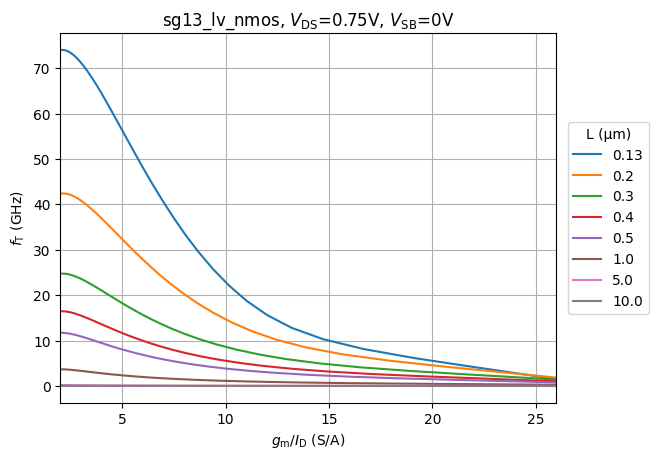
\includegraphics[keepaspectratio]{index_files/figure-latex/.-sizing-techsweep_sg13_plots_nmos-cell-9-output-1.png}}

\textsubscript{Source:
\href{https://iic-jku.github.io/analog-circuit-design/index.qmd.html}{Article
Notebook}}

The next plot shows the ratio of \(g_\mathrm{m}/ g_\mathrm{ds}\) versus
\(g_\mathrm{m}/I_\mathrm{D}\). The ratio \(g_\mathrm{m}/ g_\mathrm{ds}\)
is the so-called \textbf{``self-gain''} of the MOSFET, and shows the
maximum voltage gain we can achieve in a single transistor
configuration. As one can see the self gain increases for increasing
\(L\), but this also gives a slower transistor, so again there is a
trade-off. This plot allows us to select the proper \(L\) of a MOSFET if
we know which amount of self gain we need.

\pandocbounded{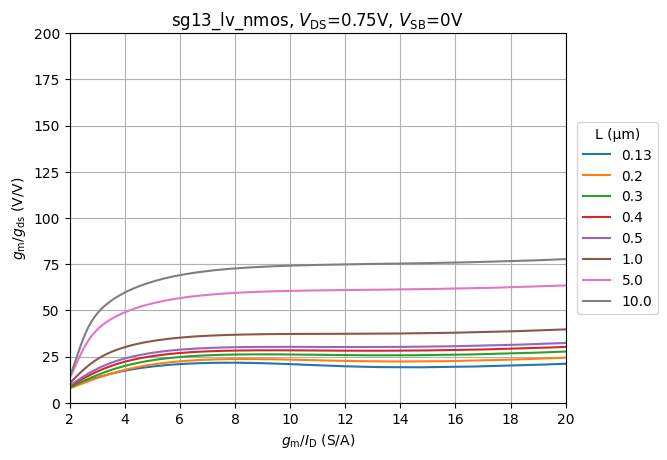
\includegraphics[keepaspectratio]{index_files/figure-latex/.-sizing-techsweep_sg13_plots_nmos-cell-10-output-1.png}}

\textsubscript{Source:
\href{https://iic-jku.github.io/analog-circuit-design/index.qmd.html}{Article
Notebook}}

The following figure plots the drain current density \(I_\mathrm{D}/W\)
as a function of \(g_\mathrm{m}/I_\mathrm{D}\) and \(L\). With this plot
we can find out how to set the \(W\) of a MOSFET once we know the
biasing current \(I_\mathrm{D}\), the \(L\) (selected according to self
gain, \(f_\mathrm{T}\), and other considerations) and the
\(g_\mathrm{m}/I_\mathrm{D}\) design point we selected. The drain
current density \(I_\mathrm{D}/W\) is a very useful normalized metric to
use, because the physical action in the MOSFET establishes a charge
density in the channel below the gate, and the changing of the \(W\) of
the device merely transforms this charge density into an absolute
parameter (together with \(L\)).

\pandocbounded{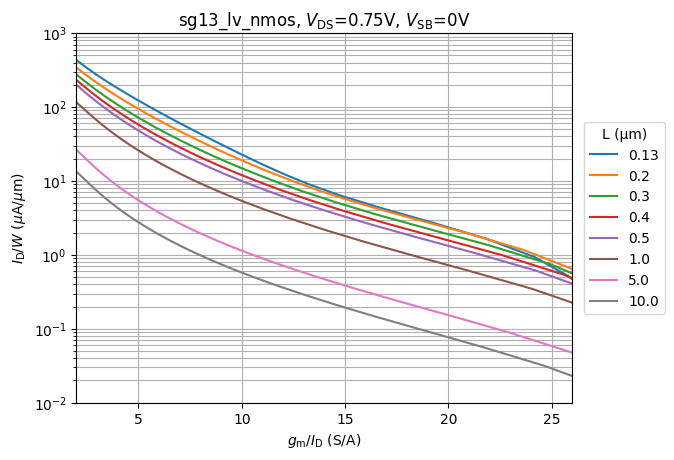
\includegraphics[keepaspectratio]{index_files/figure-latex/.-sizing-techsweep_sg13_plots_nmos-cell-11-output-1.png}}

\textsubscript{Source:
\href{https://iic-jku.github.io/analog-circuit-design/index.qmd.html}{Article
Notebook}}

The following plot shows the minimum drain-source voltage
\(V_\mathrm{ds,sat}\) that we need to establish in order to keep the
MOSFET in saturation. As you can see, this value is almost independent
of \(L\), and increases for small \(g_\mathrm{m}/I_\mathrm{D}\). So for
low-voltage circuits, where headroom is precious, we tend to bias at
\(g_\mathrm{m}/I_\mathrm{D}\ge 10\), wheres for fast circuits we need to
go to small \(g_\mathrm{m}/I_\mathrm{D}\le 5\) requiring substantial
voltage headroom per MOSFET stage that we stack on top of each other.

\pandocbounded{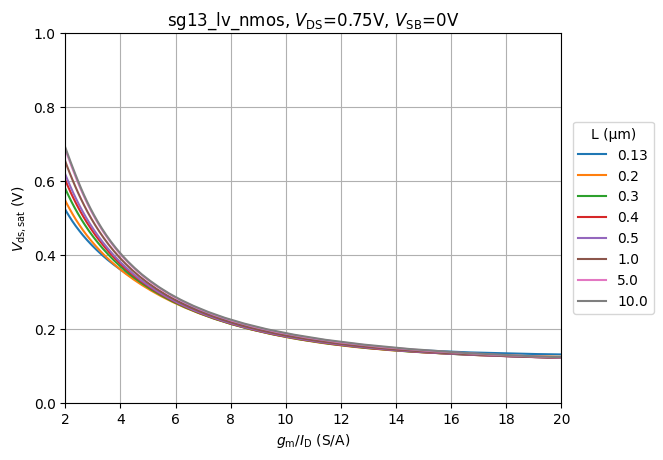
\includegraphics[keepaspectratio]{index_files/figure-latex/.-sizing-techsweep_sg13_plots_nmos-cell-12-output-1.png}}

\textsubscript{Source:
\href{https://iic-jku.github.io/analog-circuit-design/index.qmd.html}{Article
Notebook}}

For analog circuits the noise performance is usually quite important.
Thermal noise of a resistor (the Johnson-Nyquist noise) has a flat
power-spectral density (PSD) given by
\(\overline{V_\mathrm{n}^2}/\Delta f = 4 k T R\), where \(k\) is
Boltzmann's constant, \(T\) absolute temperature, and \(R\) the value of
the resistor (the unit of \(\overline{V_\mathrm{n}^2}/\Delta f\) is
\(\text{V}^2/\text{Hz}\)). This PSD is essentially flat until very high
frequencies where
\href{https://en.wikipedia.org/wiki/Johnson–Nyquist_noise}{quantum
effects} start to kick in.

\begin{tcolorbox}[enhanced jigsaw, breakable, arc=.35mm, colbacktitle=quarto-callout-note-color!10!white, toprule=.15mm, left=2mm, toptitle=1mm, bottomtitle=1mm, opacityback=0, rightrule=.15mm, opacitybacktitle=0.6, titlerule=0mm, colback=white, colframe=quarto-callout-note-color-frame, coltitle=black, title=\textcolor{quarto-callout-note-color}{\faInfo}\hspace{0.5em}{Noise Notation}, bottomrule=.15mm, leftrule=.75mm]

We usually leave the \(\Delta f\) away for a shorter notation, so we
write \(\overline{V_\mathrm{n}^2}\) when we actually mean
\(\overline{V_\mathrm{n}^2}/\Delta f\). In case of doubt look at the
unit of a quantity, whether is shows \(\text{V}^2\) or
\(\text{V}^2/\text{Hz}\) or \(\text{V}/\sqrt{\text{Hz}}\) (or
\(\text{I}^2\) or \(\text{I}^2/\text{Hz}\) or
\(\text{I}/\sqrt{\text{Hz}}\)).

Please also note that the pair of \(k T\) pretty much always shows up
together, so when you do a calculation and you miss the one or the
other, that is often a sign for miscalculation. Boltzmann's constant
\(k = 1.38 \cdot 10^{-23}\,\text{J/K}\) is just a scaling factor from
thermal energy expressed as a temperature \(T\) to energy \(E = k T\)
expressed in Joule.

Further, when working with PSD there is the usage of a one-sided
(\(0 \ge f < \infty\)) or two-sided power spectral density (PSD)
(\(-\infty < f < \infty\)). The default in this lecture is the usage of
the \textbf{one-sided PSD}.

\end{tcolorbox}

In this lecture the only MOSFET noise we consider is the drain noise (as
discussed in Section~\ref{sec-mosfet-smallsignal-model}), showing up as
a current noise between drain and source. For a realistic MOSFET noise
model, also a (correlated) gate noise component and the thermal noise of
the gate resistance needs to be considered.

The factor \(\gamma\) (Equation~\ref{eq-mosfet-noise}) is a function of
many things (in classical theory, \(\gamma = 2/3\) in saturation and
\(\gamma = 1\) in triode), and it is characterized in the following plot
as a function of \(g_\mathrm{m}/I_\mathrm{D}\) and \(L\). So when
calculating MOSFET noise we can lookup \(\gamma\) in the below plot, and
use Equation~\ref{eq-mosfet-noise} to calculate the effective drain
current noise.

\pandocbounded{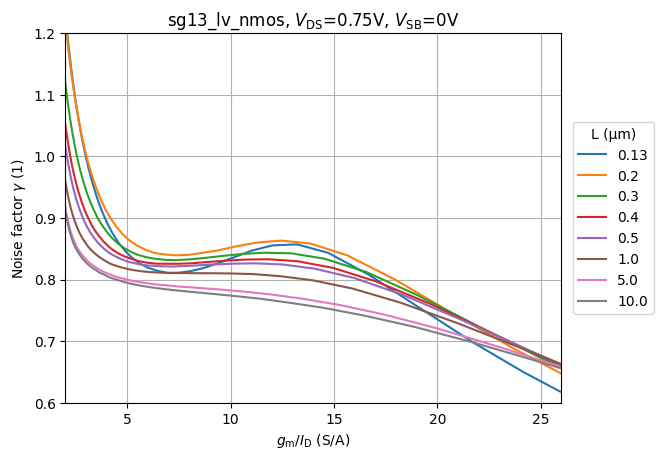
\includegraphics[keepaspectratio]{index_files/figure-latex/.-sizing-techsweep_sg13_plots_nmos-cell-13-output-1.png}}

\textsubscript{Source:
\href{https://iic-jku.github.io/analog-circuit-design/index.qmd.html}{Article
Notebook}}

In a MOSFET, unfortunately, besides the thermal noise according to
Equation~\ref{eq-mosfet-noise}, there is also a substantial
low-frequency excess noise, called ``flicker noise'' due to its
characteristic \(\overline{I_\mathrm{d,nf}^2} = K_\mathrm{f}/f\)
behavior (this means that this noise PSD decreases versus frequency). In
order to characterize this flicker noise the following plot shows the
cross-over frequency \(f_\mathrm{co}\), where the flicker noise is as
large as the thermal noise. As can be seen in the below plot, this
frequency is a strong function of \(L\) and
\(g_\mathrm{m}/I_\mathrm{D}\). Generally, the flicker noise is
proportional to \((W L)^{-1}\), so the larger the device is, the lower
the flicker noise. The parameter \(g_\mathrm{m}/I_\mathrm{D}\) largely
stays constant when we keep \(W/L\) constant, so for a given
\(g_\mathrm{m}/I_\mathrm{D}\) flicker noise is proportional to
\(1/L^2\). However, increasing \(L\) lowers device speed dramatically,
so here we have a trade-off between flicker-noise performance and MOSFET
speed, and this can have dramatic consequences for high-speed circuits.

\begin{tcolorbox}[enhanced jigsaw, breakable, arc=.35mm, colbacktitle=quarto-callout-note-color!10!white, toprule=.15mm, left=2mm, toptitle=1mm, bottomtitle=1mm, opacityback=0, rightrule=.15mm, opacitybacktitle=0.6, titlerule=0mm, colback=white, colframe=quarto-callout-note-color-frame, coltitle=black, title=\textcolor{quarto-callout-note-color}{\faInfo}\hspace{0.5em}{MOSFET Flicker Noise}, bottomrule=.15mm, leftrule=.75mm]

The physical origin of flicker noise is the crystal interface between
silicon (Si) and the silicon dioxide (SiO\textsubscript{2}). Since these
are different materials, there are dangling bonds, which can capture
charge carriers traveling in the channel. After a random time, these
carriers are released, and flicker noise is the result. The amount of
flicker noise is a function of the manufacturing process, and will
generally be different between device types and wafer foundries.

\end{tcolorbox}

As you can see in the following plot, \(f_\mathrm{co}\) can reach well
into the 10's of MHz for short MOSFETs, significantly degrading the
noise performance of a circuit.

\pandocbounded{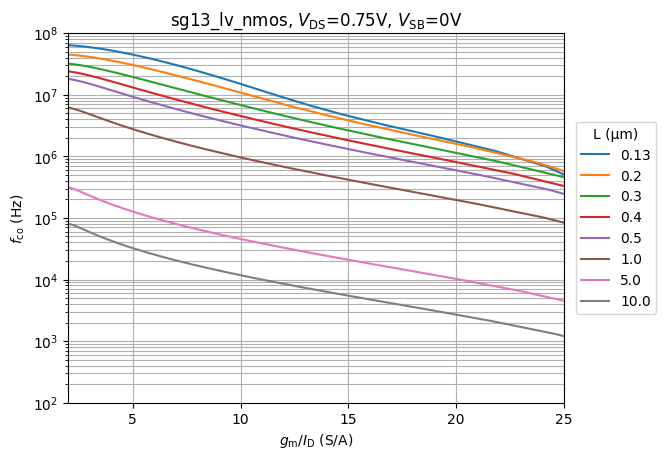
\includegraphics[keepaspectratio]{index_files/figure-latex/.-sizing-techsweep_sg13_plots_nmos-cell-14-output-1.png}}

\textsubscript{Source:
\href{https://iic-jku.github.io/analog-circuit-design/index.qmd.html}{Article
Notebook}}

During the design phase, it might be convenient to have an overview of
the most relevant sizing plots of the NMOST on one page. This overview
can be downloaded
\href{./sizing/techsweep_sg13_plots_nmos_overview/techsweep_sg13_plots_nmos_overview.pdf}{here}.

\subsection{PMOS Characterization in
Saturation}\label{sec-techsweep-pmos}

In the following, we have the same plots as discussed in
Section~\ref{sec-techsweep-nmos}, but now for the PMOS.

\begin{tcolorbox}[enhanced jigsaw, breakable, arc=.35mm, colbacktitle=quarto-callout-note-color!10!white, toprule=.15mm, left=2mm, toptitle=1mm, bottomtitle=1mm, opacityback=0, rightrule=.15mm, opacitybacktitle=0.6, titlerule=0mm, colback=white, colframe=quarto-callout-note-color-frame, coltitle=black, title=\textcolor{quarto-callout-note-color}{\faInfo}\hspace{0.5em}{PMOS Sign Convention}, bottomrule=.15mm, leftrule=.75mm]

In all PMOS plots we plot positive values for voltages and currents, to
have compatible plots to the NMOS. Of course, in a PMOS, voltages and
currents have different polarity compared to the NMOS.

\end{tcolorbox}

\(g_\mathrm{m}/I_\mathrm{D}\) and \(f_\mathrm{T}\) versus the
gate-source voltage \(V_\mathrm{GS}\):

\pandocbounded{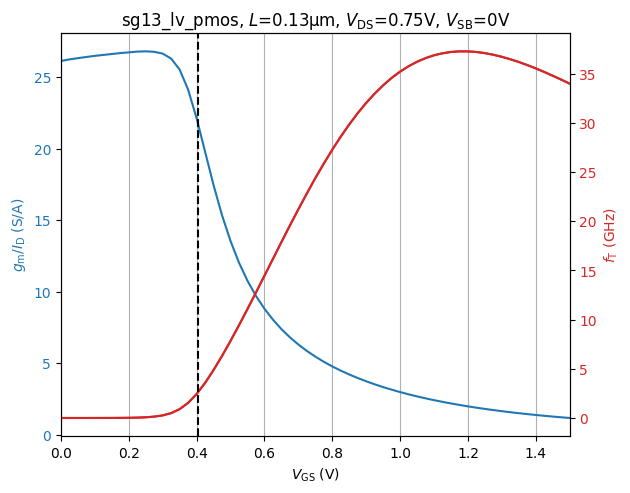
\includegraphics[keepaspectratio]{index_files/figure-latex/.-sizing-techsweep_sg13_plots_pmos-cell-6-output-1.png}}

\textsubscript{Source:
\href{https://iic-jku.github.io/analog-circuit-design/index.qmd.html}{Article
Notebook}}

\(f_\mathrm{T}\) against \(g_\mathrm{m}/I_\mathrm{D}\) for several
different \(L\). One can see a significantly lower top speed for the
PMOS compared to the NMOS, which means for high-speed circuits the NMOS
should be used. The reason for this is the approximately two to three
times higher mobility of electrons compared to the mobility of holes.

\pandocbounded{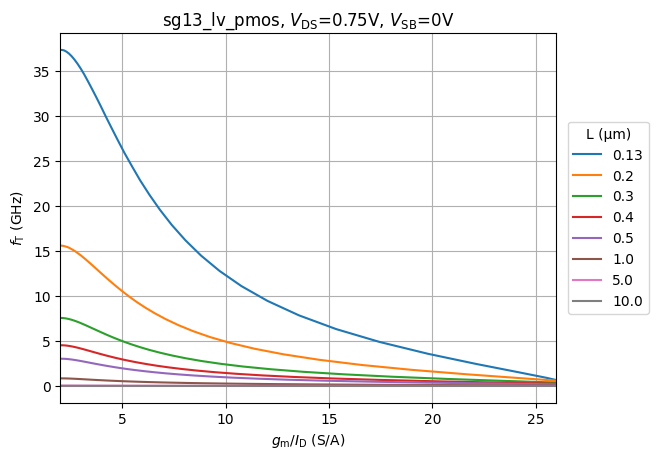
\includegraphics[keepaspectratio]{index_files/figure-latex/.-sizing-techsweep_sg13_plots_pmos-cell-9-output-1.png}}

\textsubscript{Source:
\href{https://iic-jku.github.io/analog-circuit-design/index.qmd.html}{Article
Notebook}}

\(g_\mathrm{m}/ g_\mathrm{ds}\) versus \(g_\mathrm{m}/I_\mathrm{D}\).
Unfortunately, one can see a modelling error for the PMOS in this plot.
The self gain \(g_\mathrm{m}/ g_\mathrm{ds}\) reaches non-physical
values, which indicates an issue with the \(g_\mathrm{ds}\) modelling
for the PMOS. We can not use these values for our circuit sizing, so we
will use the respective NMOS plots also for the PMOS.

\begin{tcolorbox}[enhanced jigsaw, breakable, arc=.35mm, colbacktitle=quarto-callout-important-color!10!white, toprule=.15mm, left=2mm, toptitle=1mm, bottomtitle=1mm, opacityback=0, rightrule=.15mm, opacitybacktitle=0.6, titlerule=0mm, colback=white, colframe=quarto-callout-important-color-frame, coltitle=black, title=\textcolor{quarto-callout-important-color}{\faExclamation}\hspace{0.5em}{Beware of Modelling Issues}, bottomrule=.15mm, leftrule=.75mm]

This example shows how important it is to benchmark the device models
when starting to use a new technology. Modelling artifacts like the one
shown are quite often happening, as setting up the device compact models
and parametrize them according to measurement data is a very complex
task. In any case, just be aware that modelling issues could exist in
whatever PDK you are going to use!

\end{tcolorbox}

\pandocbounded{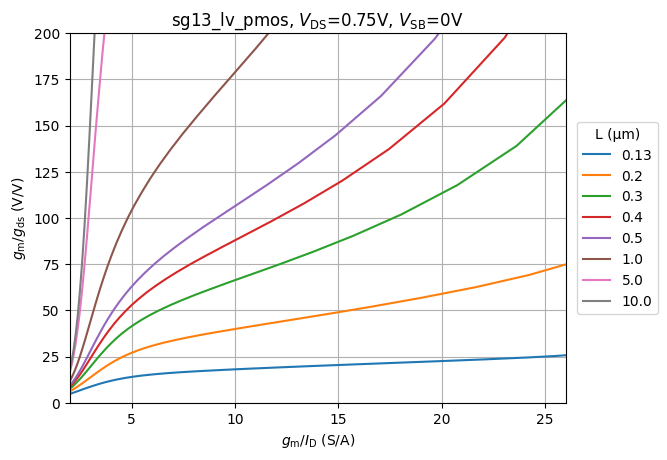
\includegraphics[keepaspectratio]{index_files/figure-latex/.-sizing-techsweep_sg13_plots_pmos-cell-10-output-1.png}}

\textsubscript{Source:
\href{https://iic-jku.github.io/analog-circuit-design/index.qmd.html}{Article
Notebook}}

Drain current density \(I_\mathrm{D}/W\) as a function of
\(g_\mathrm{m}/I_\mathrm{D}\) and \(L\):

\pandocbounded{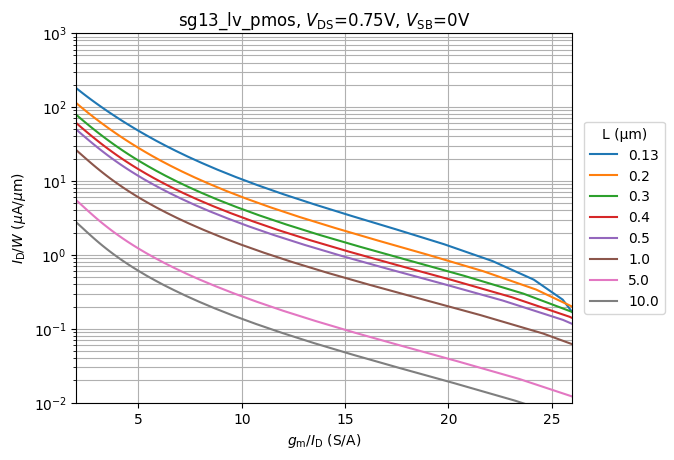
\includegraphics[keepaspectratio]{index_files/figure-latex/.-sizing-techsweep_sg13_plots_pmos-cell-11-output-1.png}}

\textsubscript{Source:
\href{https://iic-jku.github.io/analog-circuit-design/index.qmd.html}{Article
Notebook}}

Minimum drain-source voltage \(V_\mathrm{ds,sat}\) versus
\(g_\mathrm{m}/I_\mathrm{D}\) and \(L\):

\pandocbounded{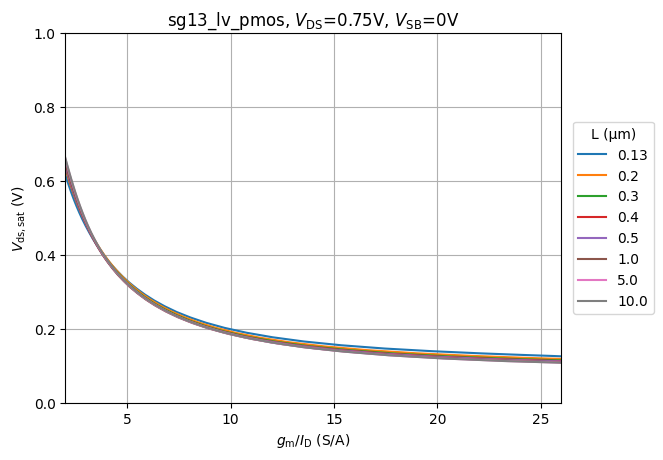
\includegraphics[keepaspectratio]{index_files/figure-latex/.-sizing-techsweep_sg13_plots_pmos-cell-12-output-1.png}}

\textsubscript{Source:
\href{https://iic-jku.github.io/analog-circuit-design/index.qmd.html}{Article
Notebook}}

Noise factor \(\gamma\) versus \(g_\mathrm{m}/I_\mathrm{D}\) and \(L\):

\pandocbounded{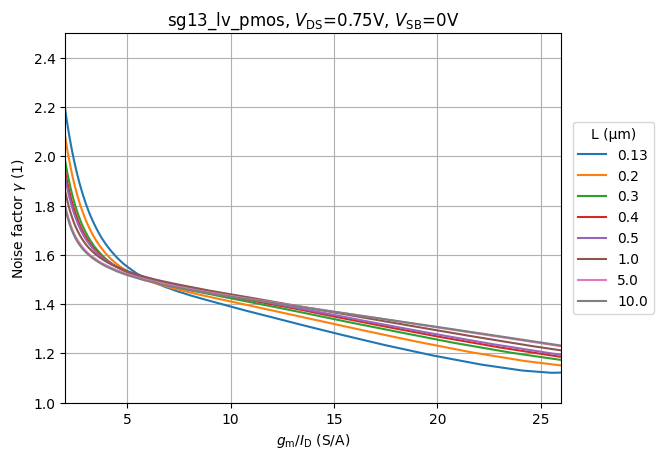
\includegraphics[keepaspectratio]{index_files/figure-latex/.-sizing-techsweep_sg13_plots_pmos-cell-13-output-1.png}}

\textsubscript{Source:
\href{https://iic-jku.github.io/analog-circuit-design/index.qmd.html}{Article
Notebook}}

Flicker noise corner frequency \(f_\mathrm{co}\) versus
\(g_\mathrm{m}/I_\mathrm{D}\) and \(L\). If you compare this figure
carefully with the NMOS figure you can see that for some operating
points the flicker noise for the PMOS is lower than for the NMOS. This
is often true for CMOS technologies, so it can be an advantage to use a
PMOS transistor in places where flicker noise is critical, like an OTA
input stage. Using PMOS has the further advantage that the bulk node can
be tied to source (which for NMOS is only possible in a triple-well
technology, which is often not available), which gets rid of the
\href{https://en.wikipedia.org/wiki/Threshold_voltage}{body effect}.

\pandocbounded{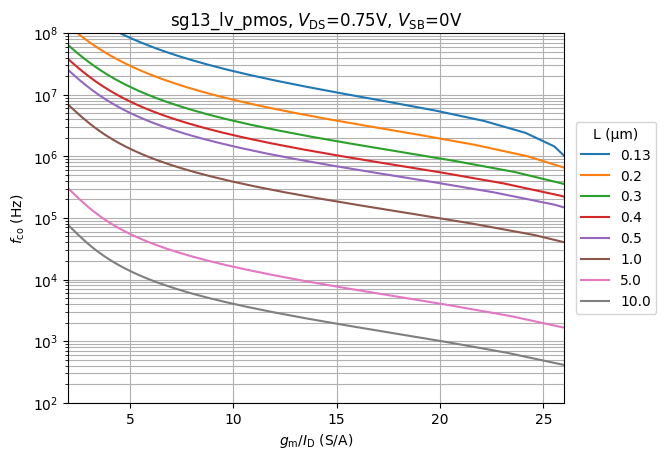
\includegraphics[keepaspectratio]{index_files/figure-latex/.-sizing-techsweep_sg13_plots_pmos-cell-14-output-1.png}}

\textsubscript{Source:
\href{https://iic-jku.github.io/analog-circuit-design/index.qmd.html}{Article
Notebook}}

During the design phase, it might be convenient to have an overview of
the most relevant sizing plots of the PMOST on one page. This overview
can be downloaded
\href{./sizing/techsweep_sg13_plots_pmos_overview/techsweep_sg13_plots_pmos_overview.pdf}{here}.

\subsection{NMOS and PMOS Characterization in
Triode}\label{nmos-and-pmos-characterization-in-triode}

Besides using the MOSFET as a transconductor in saturation we often use
the MOSFET as a switch in triode mode (to either switch voltages or
currents). In this triode/switch mode of operation we are mainly
interested in two parameters:

\begin{itemize}
\tightlist
\item
  The resistance of the switch/MOSFET when it is turned on
  (\(R_\mathrm{on} = 1 / g_\mathrm{ds}\)).
\item
  The shunt capacitance of the switch when it is turned off
  (\(C_\mathrm{off}\) is defined by the coupling capacitances between
  drain and source).
\end{itemize}

In the operation of the NMOS as a switch the gate is usually pulled to
\(V_\mathrm{DD}\) and the bulk is permanently connected to
\(V_\mathrm{SS}\) to achieve the lowest \(R_\mathrm{on}\) (to turn the
switch off the gate is pulled towards \(V_\mathrm{SS}\)). Likewise, to
turn on a PMOS, the gate is usually pulled to \(V_\mathrm{SS}\) and the
bulk is connected to \(V_\mathrm{DD}\). In this situation the
drain/source potential is somewhere between \(V_\mathrm{DD}\) and
\(V_\mathrm{SS}\), so the MOSFET will experience a
\(V_\mathrm{SB}\neq 0\), leading to a quite noticeable bulk effect. Once
the drain/source potential is sufficiently high for NMOS (low PMOS) the
switch resistance will drastically degrade.

In order to get a feeling for the behavior of the MOSFET as a switch the
following characterization plots show \(R_\mathrm{on}\) and
\(C_\mathrm{off}\) for the NMOS and the PMOS, respectively. Both plots
are for \(L = L_\mathrm{min} = 0.13\mu m\), as for switches usually
minimum length devices are used. Only for special applications (e.g.,
the drain-source leakage current in off-mode is a concern) MOSFETs with
increased \(L\) are used.

\pandocbounded{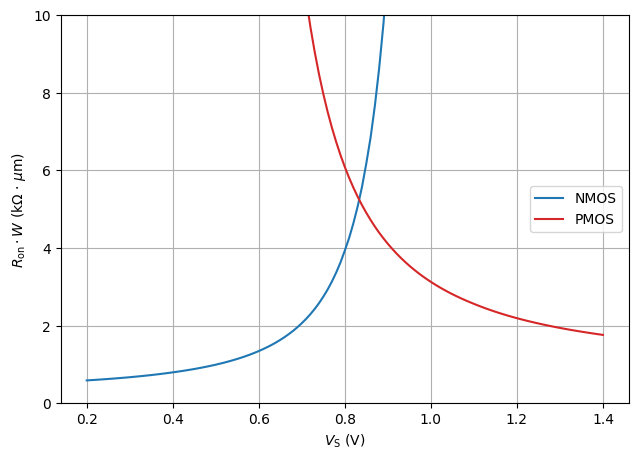
\includegraphics[keepaspectratio]{index_files/figure-latex/.-sizing-techsweep_sg13_plots_triode-cell-4-output-1.png}}

\textsubscript{Source:
\href{https://iic-jku.github.io/analog-circuit-design/index.qmd.html}{Article
Notebook}}

As can be seen in the previous plot, an NMOS can be used to switch at
potentials close to \(V_\mathrm{SS}\), while a PMOS is the better choice
when switching at potentials close to \(V_\mathrm{DD}\). To construct a
switch which can work for all voltage levels between \(V_\mathrm{DD}\)
and \(V_\mathrm{SS}\) an NMOS is put in parallel to a PMOS, resulting in
the well-known \textbf{transmission gate}.

\pandocbounded{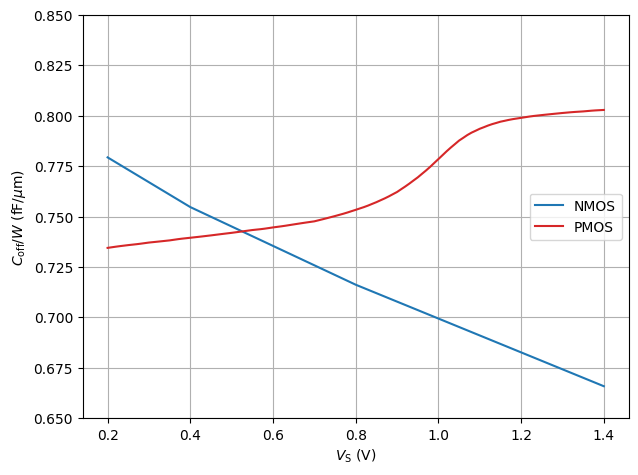
\includegraphics[keepaspectratio]{index_files/figure-latex/.-sizing-techsweep_sg13_plots_triode-cell-7-output-1.png}}

\textsubscript{Source:
\href{https://iic-jku.github.io/analog-circuit-design/index.qmd.html}{Article
Notebook}}

As the switch on-resistance gets lower when increasing \(W\), the
off-capacitance gets larger. Thus, a good performance indicator for
comparing switches in a given technology is the
\(R_\mathrm{on} C_\mathrm{off}\) product.

When designing switches, often the unwanted effects of charge injection
and clock feed-through have to be considered and, as always, a trade-off
has to be chosen. More details can be found in literature, e.g,
(Carusone, Johns, and Martin 2011) or (Razavi 2017).

\section{First Circuit: MOSFET Diode}\label{sec-mosfet-diode}

The first (simple) circuit which we will investigate is a MOSFET, where
the gate is shorted with the drain, a so-called MOSFET ``diode'', which
is shown in Figure~\ref{fig-mosfet-diode}. This diode is one half of a
current mirror, which we will investigate in
Section~\ref{sec-current-mirror}.

\textsubscript{Source:
\href{https://iic-jku.github.io/analog-circuit-design/index.qmd.html}{Article
Notebook}}

\begin{figure}[H]

\centering{

\pandocbounded{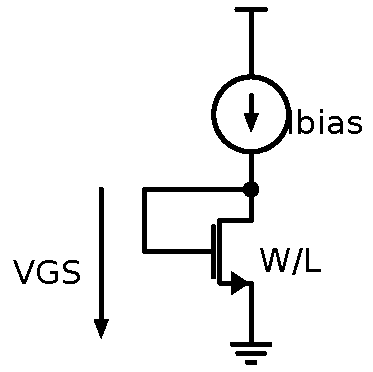
\includegraphics[keepaspectratio]{index_files/mediabag/index_files/figure-pdf/fig-mosfet-diode-output-1.pdf}}

}

\caption{\label{fig-mosfet-diode}A MOSFET connected as a diode (drain
shorted with gate).}

\end{figure}%

\textsubscript{Source:
\href{https://iic-jku.github.io/analog-circuit-design/index.qmd.html}{Article
Notebook}}

Why looking at a single-transistor circuit at all? By starting with the
simplest possible circuit we can develop important skills in circuit
analysis (setting up and calculating a small-signal model, calculating
open-loop gain, calculate noise, etc.) and Xschem/ngspice simulation
testbench creation. We safely assume that also the Mona Lisa was not
Leonardo da Vinci's first painting, so let's start slow.

This diode is usually biased by a current source, shown as
\(I_\mathrm{bias}\) in the figure. Depending on MOSFET sizing with \(W\)
and \(L\), a certain gate-source voltage \(V_\mathrm{GS}\) will develop.
This voltage can be used as a biasing voltage for other circuit parts,
for example.

\begin{tcolorbox}[enhanced jigsaw, breakable, arc=.35mm, colbacktitle=quarto-callout-note-color!10!white, toprule=.15mm, left=2mm, toptitle=1mm, bottomtitle=1mm, opacityback=0, rightrule=.15mm, opacitybacktitle=0.6, titlerule=0mm, colback=white, colframe=quarto-callout-note-color-frame, coltitle=black, title=\textcolor{quarto-callout-note-color}{\faInfo}\hspace{0.5em}{Feedback in the MOSFET Diode}, bottomrule=.15mm, leftrule=.75mm]

It is important to realize that this configuration employs a feedback
loop for operation. The voltage at the drain of the MOSFET is sensed by
the gate, and the gate voltage changes until \(I_\mathrm{D}\) is exactly
equal to \(I_\mathrm{bias}\). In this sense this is probably the
smallest feedback circuit one can build.

\end{tcolorbox}

\subsection{MOSFET Diode Sizing}\label{mosfet-diode-sizing}

We will now build this circuit in Xschem. For sizing the MOSFET we will
use the \(g_\mathrm{m}/I_\mathrm{D}\) methodology introduced in
Section~\ref{sec-gmid-method}.

\begin{tcolorbox}[enhanced jigsaw, breakable, arc=.35mm, colbacktitle=quarto-callout-tip-color!10!white, toprule=.15mm, left=2mm, toptitle=1mm, bottomtitle=1mm, opacityback=0, rightrule=.15mm, opacitybacktitle=0.6, titlerule=0mm, colback=white, colframe=quarto-callout-tip-color-frame, coltitle=black, title=\textcolor{quarto-callout-tip-color}{\faLightbulb}\hspace{0.5em}{Exercise: MOSFET Diode Sizing}, bottomrule=.15mm, leftrule=.75mm]

Please build a MOSFET diode circuit in Xschem where you use an LV NMOS,
set \(I_\mathrm{bias} = 20\,\mu\text{A}\), \(L = 0.13\,\mu\text{m}\),
and we want to use \(g_\mathrm{m}/I_\mathrm{D}= 10\) (often a suitable
compromise between transistor speed and \(g_\mathrm{m}\) efficiency).

\begin{enumerate}
\def\labelenumi{\arabic{enumi}.}
\tightlist
\item
  Use the figures in Section~\ref{sec-techsweep-nmos} to find out the
  proper value for \(W\).
\item
  What is the \(f_\mathrm{T}\) for this MOSFET? What is the value for
  \(g_\mathrm{m}\) and \(g_\mathrm{ds}\)?
\item
  Draw the circuit in Xschem, and simulate the operating point. Do the
  values match to the values found out before during circuit sizing?
\end{enumerate}

\end{tcolorbox}

Before continuing, please finish the previous exercise. Once you are
done, compare with the below provided solution.

\begin{tcolorbox}[enhanced jigsaw, breakable, arc=.35mm, colbacktitle=quarto-callout-tip-color!10!white, toprule=.15mm, left=2mm, toptitle=1mm, bottomtitle=1mm, opacityback=0, rightrule=.15mm, opacitybacktitle=0.6, titlerule=0mm, colback=white, colframe=quarto-callout-tip-color-frame, coltitle=black, title=\textcolor{quarto-callout-tip-color}{\faLightbulb}\hspace{0.5em}{Solution: MOSFET Diode Sizing}, bottomrule=.15mm, leftrule=.75mm]

\begin{enumerate}
\def\labelenumi{\arabic{enumi}.}
\tightlist
\item
  Using the fact that
  \(I_\mathrm{bias} = I_\mathrm{D} = 20\,\mu\text{A}\) and
  \(g_\mathrm{m}/I_\mathrm{D}= 10\) directly provides
  \(g_\mathrm{m}= 0.2\,\text{mS}\).
\item
  Using the self-gain plot, we see that
  \(g_\mathrm{m}/g_\mathrm{ds}\approx 21\), so
  \(g_\mathrm{ds}\approx 9.5\,\mu\text{S}\). The \(f_\mathrm{T}\) can
  easily be found in the respective plot to be
  \(f_\mathrm{T} = 23\,\text{GHz}\).
\item
  The \(W\) of the MOSFET we find using the drain current density plot
  and the given bias current. Rounding to half-microns results in
  \(W = 1\,\mu\text{m}\).
\item
  Since we are looking at the graphs, we further find \(\gamma = 0.84\),
  \(V_\mathrm{ds,sat} = 0.18\,\text{V}\), and
  \(f_\mathrm{co} \approx 15\,\text{MHz}\).
\item
  In addition, we expect \(V_\mathrm{GS}\approx 0.6\,\text{V}\).
\end{enumerate}

An example Jupyter notebook to extract these values accurately you can
find \href{./sizing/sizing_mosfet_diode.ipynb}{here}. An Xschem
schematic for this exercise is provide
\href{./xschem/mosfet_diode_sizing.sch}{as well}.

\end{tcolorbox}

\subsection{MOSFET Diode Large-Signal
Behavior}\label{mosfet-diode-large-signal-behavior}

As discussed above, the MOSFET diode configuration is essentially a
feedback loop. Before we will analyze this loop in small-signal, we want
to investigate how this loop settles in the time domain, and by doing
this we can observe the large-signal settling behavior. To simulate
this, we change the dc bias source from the previous example to a
transient current source, which we will turn on after some picoseconds.
The resulting Xschem testbench is shown in
Figure~\ref{fig-mosfet-diode-settling-tb}.

\begin{figure}

\centering{

\pandocbounded{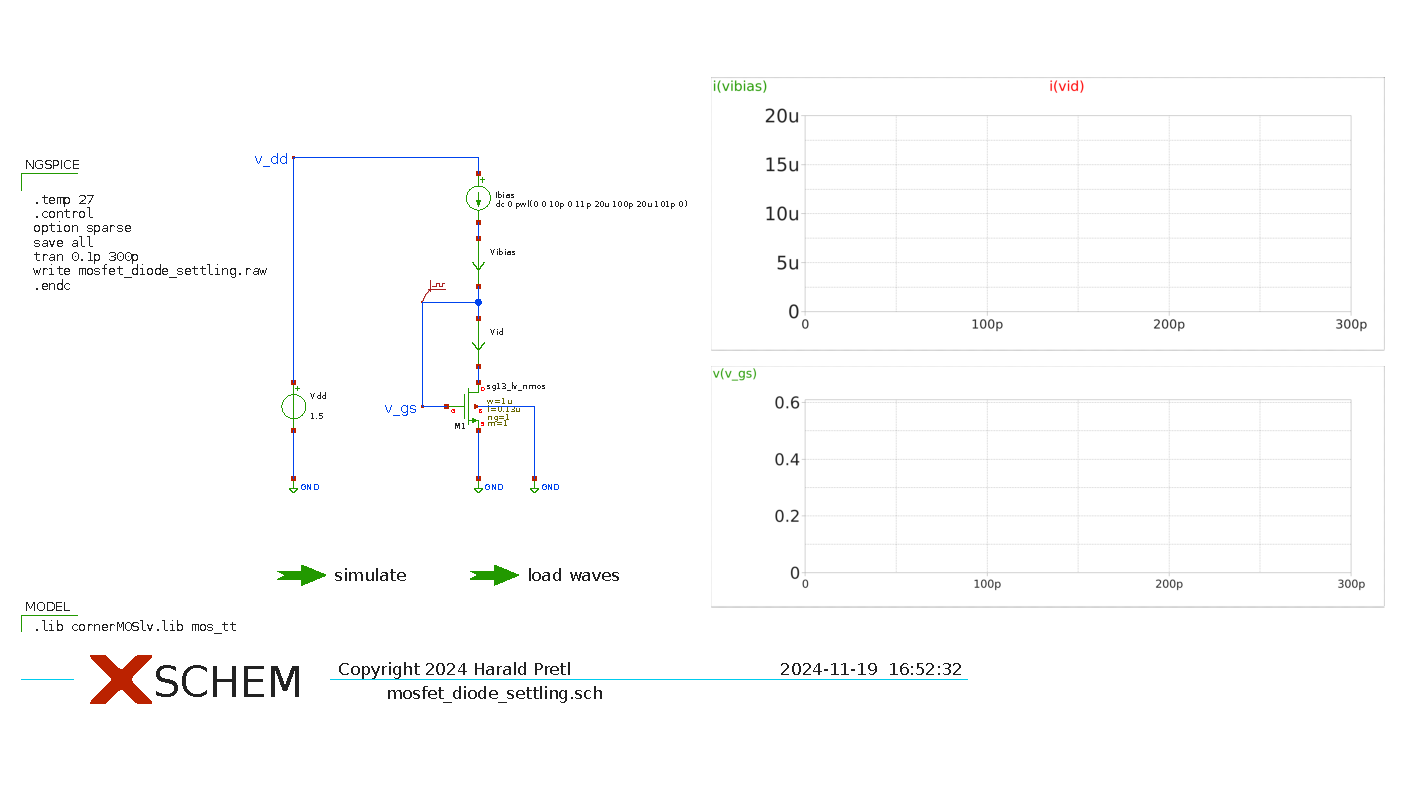
\includegraphics[keepaspectratio]{index_files/mediabag/xschem/mosfet_diode_settling.pdf}}

}

\caption{\label{fig-mosfet-diode-settling-tb}Testbench for MOSFET diode
transient settling.}

\end{figure}%

When simulating the circuit in Figure~\ref{fig-mosfet-diode-settling-tb}
another interesting effect can be observed: While the turn-on happens
quite rapidly (essentially the bias current source charges the gate
capacitance, until the gate-source voltage is large enough that the
drain current counteracts the bias current), the turn-off shows a very
long settling tail. This is due to the fact that as the gate capacitance
is discharged by the drain current, the \(V_\mathrm{GS}\) drops, which
in turn reduces the drain current, which will make the discharge even
slower. We have an effect similar to a capacitor discharge by a diode
(Hellen 2003).

\begin{tcolorbox}[enhanced jigsaw, breakable, arc=.35mm, colbacktitle=quarto-callout-important-color!10!white, toprule=.15mm, left=2mm, toptitle=1mm, bottomtitle=1mm, opacityback=0, rightrule=.15mm, opacitybacktitle=0.6, titlerule=0mm, colback=white, colframe=quarto-callout-important-color-frame, coltitle=black, title=\textcolor{quarto-callout-important-color}{\faExclamation}\hspace{0.5em}{Power-Down Switches}, bottomrule=.15mm, leftrule=.75mm]

It is thus generally a good idea to add power-down switches to the
circuits to disable the circuit quickly by pulling floating nodes to a
defined potential (usually \(V_\mathrm{DD}\) or \(V_\mathrm{SS}\)) and
to avoid long intermediate states during power down. This will also
allow a turn-on from a well-defined off-state.

\end{tcolorbox}

Exemplary implementations of power-down switches are shown in the Xschem
implementation of the improved OTA in
Figure~\ref{fig-improved-ota-design}. Which \(W/L\) ratio should these
transistors have? Well, in general, switches often have minimum length
to be fast and to have low \(R_\mathrm{on}\). However, if there are no
critical specifications (e.g., like power-down time), then these
transistors are often used as dummy transistors for other circuit parts
and are sized to fit the layout best.

\subsection{MOSFET Diode Small-Signal
Analysis}\label{mosfet-diode-small-signal-analysis}

We now want to investigate the small-signal behavior of the MOSFET
diode. Based on the small-signal model of the MOSFET in
Figure~\ref{fig-mosfet-small-signal-model} we realize that gate and
drain are shorted, and we also connect bulk to source. We can thus
simplify the circuit to the one shown in
Figure~\ref{fig-mosfet-diode-small-signal}.

\textsubscript{Source:
\href{https://iic-jku.github.io/analog-circuit-design/index.qmd.html}{Article
Notebook}}

\begin{figure}[H]

\centering{

\pandocbounded{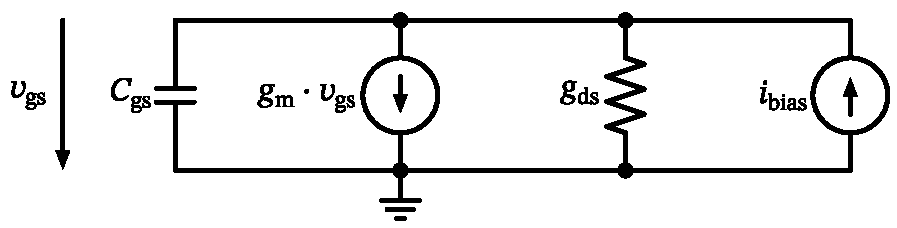
\includegraphics[keepaspectratio]{index_files/mediabag/index_files/figure-pdf/fig-mosfet-diode-small-signal-output-1.pdf}}

}

\caption{\label{fig-mosfet-diode-small-signal}The MOSFET diode
small-signal model (drain and gate are shorted, as well as source and
bulk).}

\end{figure}%

\textsubscript{Source:
\href{https://iic-jku.github.io/analog-circuit-design/index.qmd.html}{Article
Notebook}}

\begin{tcolorbox}[enhanced jigsaw, breakable, arc=.35mm, colbacktitle=quarto-callout-note-color!10!white, toprule=.15mm, left=2mm, toptitle=1mm, bottomtitle=1mm, opacityback=0, rightrule=.15mm, opacitybacktitle=0.6, titlerule=0mm, colback=white, colframe=quarto-callout-note-color-frame, coltitle=black, title=\textcolor{quarto-callout-note-color}{\faInfo}\hspace{0.5em}{Ground Node Selection}, bottomrule=.15mm, leftrule=.75mm]

For small-signal analysis we would not need to declare one node as the
ground potential. However, when doing so, and selecting the ground node
strategically, we can simplify the analysis, as we usually do not
formulate KCL for the ground node (as we have only \(N-1\) independent
KCL equations, \(N\) being the number of nodes in the circuit), and the
potential difference equations are simpler if one node is at \(0\,V\).

\end{tcolorbox}

For calculating the small-signal impedance of the MOSFET diode we
formulate Kirchhoff's current law (KCL, also Kirchhoff's first law or
Kirchhoff's junction rule) at the top node to get \[
i_\mathrm{bias} - s C_\mathrm{gs}v_\mathrm{gs}- g_\mathrm{m}v_\mathrm{gs}- g_\mathrm{ds}v_\mathrm{gs}= 0.
\]

It follows that
\begin{equation}\phantomsection\label{eq-mosfet-diode-impedance}{
Z_\mathrm{diode}(s) = \frac{v_\mathrm{gs}}{i_\mathrm{bias}} = \frac{1}{g_\mathrm{m}+ g_\mathrm{ds}+ s C_\mathrm{gs}}.
}\end{equation}

When neglecting \(g_\mathrm{ds}\), at dc we get
\(Z_\mathrm{diode} = 1 / g_\mathrm{m}\), which is an important result
and should be memorized.

\begin{tcolorbox}[enhanced jigsaw, breakable, arc=.35mm, colbacktitle=quarto-callout-important-color!10!white, toprule=.15mm, left=2mm, toptitle=1mm, bottomtitle=1mm, opacityback=0, rightrule=.15mm, opacitybacktitle=0.6, titlerule=0mm, colback=white, colframe=quarto-callout-important-color-frame, coltitle=black, title=\textcolor{quarto-callout-important-color}{\faExclamation}\hspace{0.5em}{The Admittance is Your Friend}, bottomrule=.15mm, leftrule=.75mm]

In circuit analysis it is often algebraically easier to work with
admittance instead of impedance, so please remember that Ohm's law for a
conductance is \(I = G \cdot V\), and for a capacitance is
\(I = s C \cdot V\). When writing equations, it is also practical to
keep \(s C\) together, so we will strive to sort terms accordingly.

\end{tcolorbox}

Looking at Equation~\ref{eq-mosfet-diode-impedance} we see that for low
frequencies, the diode impedance is resistive, and for high frequencies
it becomes capacitive as the gate-source capacitance starts to dominate.
The corner frequency of this low-pass can be calculated as \[
\omega_\mathrm{c} = \frac{g_\mathrm{m}+ g_\mathrm{ds}}{C_\mathrm{gs}} \approx \omega_\mathrm{T}
\] which is pretty much the transit frequency of the MOSFET!

\subsection{MOSFET Diode Stability
Analysis}\label{mosfet-diode-stability-analysis}

\begin{tcolorbox}[enhanced jigsaw, breakable, arc=.35mm, colbacktitle=quarto-callout-note-color!10!white, toprule=.15mm, left=2mm, toptitle=1mm, bottomtitle=1mm, opacityback=0, rightrule=.15mm, opacitybacktitle=0.6, titlerule=0mm, colback=white, colframe=quarto-callout-note-color-frame, coltitle=black, title=\textcolor{quarto-callout-note-color}{\faInfo}\hspace{0.5em}{Open-Loop Gain, Closed-Loop Gain, and Loop-Gain---A Short Recap}, bottomrule=.15mm, leftrule=.75mm]

Figure~\ref{fig-feedback-system} shows a negative feedback system with
input \(X(s)\) and output \(Y(s)\), where \(H_\mathrm{ol}(s)\) is the
transfer function of the feed-forward path (also called
\textbf{open-loop gain}) and \(G(s)\) is the transfer function of the
feedback network. The \textbf{loop-gain} is the product of both transfer
functions \(T(s) = H_\mathrm{ol}(s) G(s)\) and is used for the stability
analysis. The \textbf{closed-loop} gain is defined as
\(H_\mathrm{cl}(s) = Y(s) / X(s)\) can be derived with
\(Y(s) = H_\mathrm{ol}(s) [X(s) - Y(s) G(s)]\) to be
\begin{equation}\phantomsection\label{eq-closed-loop-gain}{
H_\mathrm{cl}(s) = \frac{Y(s)}{X(s)} = \frac{H_\mathrm{ol}(s)}{1 + H_\mathrm{ol}(s) G(s)} = \frac{H_\mathrm{ol}(s)}{1 + T(s)}
}\end{equation}

If the open-loop gain is sufficiently large \(H_\mathrm{ol}(s) \gg 1\),
then the closed-loop gain simplifies to
\(H_\mathrm{cl}(s) \approx 1 / G(s)\). This result is convenient, since
it is independent of \(H_\mathrm{ol}(s)\). Therefore, the overall gain
is only set with the feedback gain \(G(s)\) in operational amplifier
circuits.

In the case of the MOSFET diode, \(G(s) = 1\) and therefore
\(T(s) = H_\mathrm{ol}(s)\) and \(H_\mathrm{cl}(s) \approx 1\).
Therefore, this chapter uses open-loop gain and loop-gain as synonyms.

\end{tcolorbox}

\begin{figure}[H]

\centering{

\pandocbounded{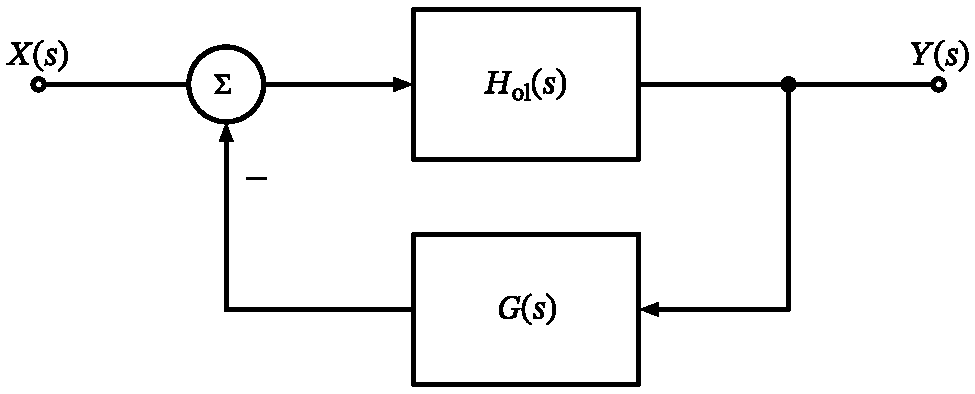
\includegraphics[keepaspectratio]{index_files/mediabag/index_files/figure-pdf/fig-feedback-system-output-1.pdf}}

}

\caption{\label{fig-feedback-system}The block diagram of a negative
feedback system.}

\end{figure}%

\begin{tcolorbox}[enhanced jigsaw, breakable, arc=.35mm, colbacktitle=quarto-callout-note-color!10!white, toprule=.15mm, left=2mm, toptitle=1mm, bottomtitle=1mm, opacityback=0, rightrule=.15mm, opacitybacktitle=0.6, titlerule=0mm, colback=white, colframe=quarto-callout-note-color-frame, coltitle=black, title=\textcolor{quarto-callout-note-color}{\faInfo}\hspace{0.5em}{Gain-Bandwidth Product in Feedback Systems}, bottomrule=.15mm, leftrule=.75mm]

The gain-bandwidth product (GBP or GBWP) or transit frequency
\(f_\mathrm{T}\) of a first-order open-loop system is the product of the
open-loop dc gain \(H_\mathrm{ol,dc} = H_\mathrm{ol}(f = 0\,\text{Hz})\)
and the open-loop \(-3\,\text{dB}\) cut-off frequency
\(f_\mathrm{c,ol}\) of \(H_\mathrm{ol}(s)\). \[
\text{GBWP} = f_\mathrm{T,ol} = H_\mathrm{ol,dc} f_\mathrm{c,ol}
\]

If a frequency-independent negative feedback \(G\) (e.g., a resistive
divider) is applied to this open-loop system, the transit frequency
changes to \[
f_\mathrm{T,cl} = f_\mathrm{T,ol} \sqrt{1 - G^2}
\] Hence, the closed-loop transit frequency is slightly lower than the
open-loop transit frequency \(f_\mathrm{T,cl} < f_\mathrm{T,ol}\).

The closed-loop \(-3\,\text{dB}\) cut-off frequency \(f_\mathrm{c,cl}\)
can then be calculated from the open-loop transit frequency and the
feedback gain. \[
f_\mathrm{c,cl} = H_\mathrm{ol,DC} f_\mathrm{c,ol} G = f_\mathrm{T,ol} G
\]

This theory might be interesting when Middlebrook's and Tian's methods
for loop gain analysis are later compared in the MOSFET diode testbench
(see Figure~\ref{fig-mosfet-diode-loopgain-tb}).

\end{tcolorbox}

The diode-connected MOSFET forms a feedback loop. What is the open-loop
gain? For calculating it, we are breaking the loop, and apply a dummy
\(C_\mathrm{gs}^{*}\) at the right side to keep the impedances correct.
A circuit diagram is shown in Figure~\ref{fig-mosfet-diode-openloop}, we
break the loop at the dotted connection. As we can see in this example,
it is critically important when breaking up a loop for analysis (also
for simulation!) to keep the terminal impedances the same. Only in
special cases where the load impedance is very high or the driving
impedance is very low is it acceptable to disregard loading effects!

\textsubscript{Source:
\href{https://iic-jku.github.io/analog-circuit-design/index.qmd.html}{Article
Notebook}}

\begin{figure}[H]

\centering{

\pandocbounded{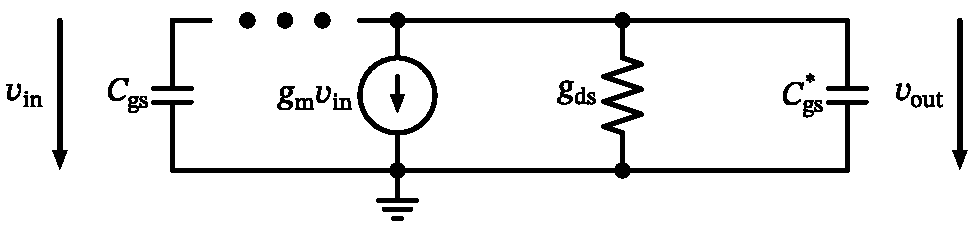
\includegraphics[keepaspectratio]{index_files/mediabag/index_files/figure-pdf/fig-mosfet-diode-openloop-output-1.pdf}}

}

\caption{\label{fig-mosfet-diode-openloop}The MOSFET diode small-signal
circuit for open-loop analysis.}

\end{figure}%

\textsubscript{Source:
\href{https://iic-jku.github.io/analog-circuit-design/index.qmd.html}{Article
Notebook}}

We are now driving (with a voltage source) \(v_\mathrm{in}\) and record
the output voltage \(v_\mathrm{out}\) to find the open-loop response
\(H_\mathrm{ol}(s)\). By inspecting
Figure~\ref{fig-mosfet-diode-openloop} we see that \[
v_\mathrm{out} = - g_\mathrm{m}v_\mathrm{in} \frac{1}{g_\mathrm{ds}+ s C_\mathrm{gs}}.
\]

The open-loop gain \(H_\mathrm{ol}(s)\) is thus
\begin{equation}\phantomsection\label{eq-mosfet-diode-openloop-gain}{
H_\mathrm{ol}(s) = \frac{v_\mathrm{out}}{v_\mathrm{in}} = -\frac{g_\mathrm{m}}{g_\mathrm{ds}+ s C_\mathrm{gs}} = - \frac{g_\mathrm{m}}{g_\mathrm{ds}} \frac{1}{1 + s \frac{C_\mathrm{gs}}{g_\mathrm{ds}}}.
}\end{equation}

Inspecting Equation~\ref{eq-mosfet-diode-openloop-gain} we realize that:

\begin{enumerate}
\def\labelenumi{\arabic{enumi}.}
\tightlist
\item
  The dc gain \(g_\mathrm{m}/ g_\mathrm{ds}\) is the self-gain of the
  MOSFET, so
  \(20 \log_{10}(0.2 \cdot 10^{-3} / 9.6 \cdot 10 ^{-6}) = 26.4\,\text{dB}\).
\item
  There is a pole at
  \(\omega_\mathrm{p} = -g_\mathrm{ds}/ C_\mathrm{gs}\), which is at
  \(9.6 \cdot 10 ^{-6} / (2 \pi \cdot 1.4 \cdot 10^{-15}) = 1.1\,\text{GHz}\).
\end{enumerate}

With this single pole location in \(H_\mathrm{ol}(s)\) this loop is
perfectly stable at under all conditions (remember that a single pole
results in a maximum phase shift of --90\(^\circ\)).

The question is now how to simulate this open-loop gain, i.e., how to
break the loop open in simulation? In general there are various methods,
as we can use artificially large (ideal) inductors and capacitors to
break loops open and still establish the correct dc operating points for
the ac loop analysis. This is called \textbf{Rosenstark's method}
(Rosenstark 1984). However, mimicking the correct loading can be an
issue, and requires a lot of careful consideration.

There is an alternative method which breaks the loop open only by adding
an ac voltage source in series (thus keeps the dc operating point
intact), or injects current using an ac current source. Based on both
measurements the open-loop gain can be calculated. This is called
\textbf{Middlebrook's method} (Middlebrook 1975) and is based on double
injection, and we will use it for our loop simulations. This method is
detailed in Section~\ref{sec-middlebrook-method}.

There are several other methods like Tian's method (Tian et al. 2001),
for example. A comprehensive overview can be found in (Neag et al. 2015)
which describes ten different simulation-based loop gain analysis
methods.

We now want to simulate the open-loop transfer function
\(H_\mathrm{ol}(s)\) by using Middlebrook's method and confirm our
analysis above.

\begin{tcolorbox}[enhanced jigsaw, breakable, arc=.35mm, colbacktitle=quarto-callout-tip-color!10!white, toprule=.15mm, left=2mm, toptitle=1mm, bottomtitle=1mm, opacityback=0, rightrule=.15mm, opacitybacktitle=0.6, titlerule=0mm, colback=white, colframe=quarto-callout-tip-color-frame, coltitle=black, title=\textcolor{quarto-callout-tip-color}{\faLightbulb}\hspace{0.5em}{Exercise: MOSFET Diode Loop Analysis}, bottomrule=.15mm, leftrule=.75mm]

Please build a simulation testbench in Xschem to simulate the open-loop
transfer function of the MOSFET diode. Confirm the dc gain and pole
location as given by Equation~\ref{eq-mosfet-diode-openloop-gain}.

If you are getting stuck you can look at this Xschem
\href{./xschem/mosfet_diode_loopgain.sch}{testbench}, shown in
Figure~\ref{fig-mosfet-diode-loopgain-tb}.

\begin{figure}[H]

\centering{

\pandocbounded{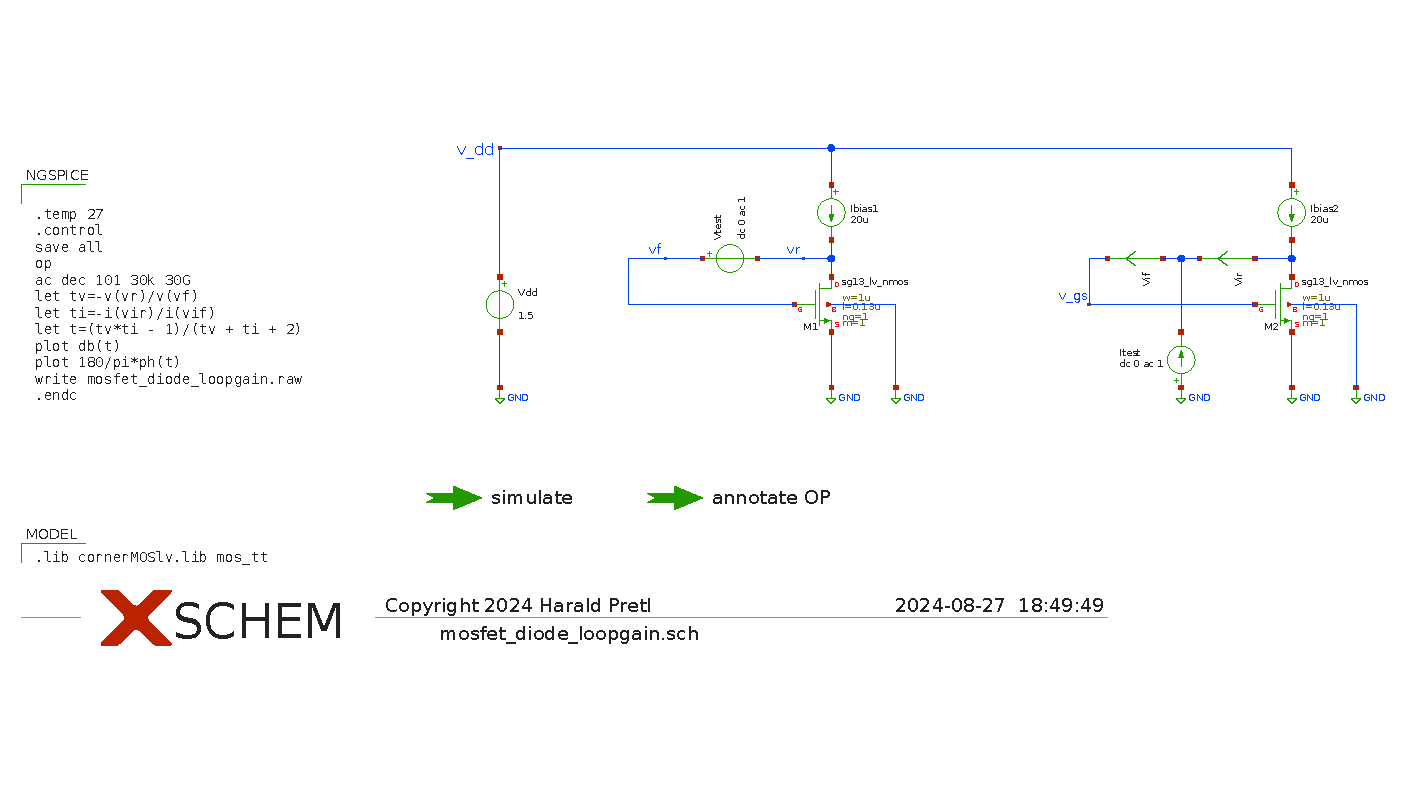
\includegraphics[keepaspectratio]{index_files/mediabag/xschem/mosfet_diode_loopgain.pdf}}

}

\caption{\label{fig-mosfet-diode-loopgain-tb}Testbench for MOSFET diode
stability analysis.}

\end{figure}%

\end{tcolorbox}

From simulation we see that the open-loop gain is \(24.9\,\text{dB}\) at
low frequencies, which matches quite well our prediction of
\(26.4\,\text{dB}\). In the Bode plot we see a low-pass with a
\(-3\,\text{dB}\) corner frequency of \(1.4\,\text{GHz}\), which again
is fairly close to our prediction of \(1.1\,\text{GHz}\).

\begin{tcolorbox}[enhanced jigsaw, breakable, arc=.35mm, colbacktitle=quarto-callout-important-color!10!white, toprule=.15mm, left=2mm, toptitle=1mm, bottomtitle=1mm, opacityback=0, rightrule=.15mm, opacitybacktitle=0.6, titlerule=0mm, colback=white, colframe=quarto-callout-important-color-frame, coltitle=black, title=\textcolor{quarto-callout-important-color}{\faExclamation}\hspace{0.5em}{What About Large-Signal Stability?}, bottomrule=.15mm, leftrule=.75mm]

Keep in mind that the above simulation only verifies the small-signal
stability in one certain operating point. If we later look at the
stability of an OTA it might be a good idea to verify the small-signal
stability in different operating points.

Furthermore, one can apply a step response to the closed-loop system
input and estimate the phase margin from the overshoot at the output
(see \emph{``Automatic Control''} lecture). One could also use a
step-wise step response to simulate different operating points for a
certain time (see \emph{``Introduction in Integrated Circuit Design''}
lecture).

\end{tcolorbox}

\subsection{MOSFET Diode Noise
Calculation}\label{mosfet-diode-noise-calculation}

As a final exercise on the MOSFET diode circuit we want to calculate the
output noise when we consider \(V_\mathrm{GS}\) the output reference
voltage which is created when passing a bias current through the MOSFET
diode. The bias current we will assume noiseless.

We are going to use the small-signal circuit shown in
Figure~\ref{fig-mosfet-diode-small-signal-w-noise}.

\textsubscript{Source:
\href{https://iic-jku.github.io/analog-circuit-design/index.qmd.html}{Article
Notebook}}

\begin{figure}[H]

\centering{

\pandocbounded{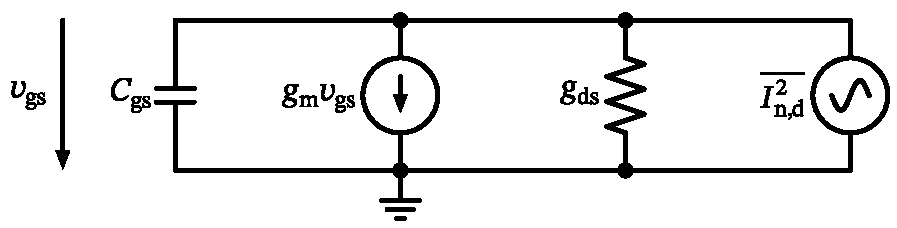
\includegraphics[keepaspectratio]{index_files/mediabag/index_files/figure-pdf/fig-mosfet-diode-small-signal-w-noise-output-1.pdf}}

}

\caption{\label{fig-mosfet-diode-small-signal-w-noise}The MOSFET diode
small-signal model with drain noise source.}

\end{figure}%

\textsubscript{Source:
\href{https://iic-jku.github.io/analog-circuit-design/index.qmd.html}{Article
Notebook}}

As we have already calculated the small-signal diode impedance in
Equation~\ref{eq-mosfet-diode-impedance} we will use this result, and
just note that the drain current noise of the MOSFET flows through this
impedance. The noise voltage at \(v_\mathrm{gs}\) is thus given as \[
\overline{V_\mathrm{n}^2} = |Z_\mathrm{diode}|^2 \overline{I_\mathrm{n,d}^2}.
\]

The drain current noise of the MOSFET is given as (introduced in
Section~\ref{sec-mosfet-smallsignal-model}) \[
\overline{I_\mathrm{n,d}^2} = 4 k T \gamma g_\mathrm{m}.
\]

For low frequencies (ignoring \(g_\mathrm{ds}\) and \(C_\mathrm{gs}\))
we get \[
\overline{V_\mathrm{n}^2} = |Z_\mathrm{diode}|^2 \overline{I_\mathrm{n,d}^2} = \frac{1}{g_\mathrm{m}^2} 4 k T \gamma g_\mathrm{m}= \frac{4 k T \gamma}{g_\mathrm{m}}
\] which is the thermal noise of a resistor of value
\(1 / g_\mathrm{m}\) enhanced by the factor \(\gamma\).

We now calculate the full equation, and after a bit of algebra arrive at
\begin{equation}\phantomsection\label{eq-mosfet-diode-noise-psd}{
\overline{V_\mathrm{n}^2}(f) = \frac{4 k T \gamma g_\mathrm{m}}{(g_\mathrm{m}+ g_\mathrm{ds})^2 + (2 \pi f C_\mathrm{gs})^2}.
}\end{equation}

If we are interested in the PSD of the noise then
Equation~\ref{eq-mosfet-diode-noise-psd} gives us the result. If we are
interested in the rms value (the total noise) we need to integrate this
equation, using the following identity:

\begin{tcolorbox}[enhanced jigsaw, breakable, arc=.35mm, colbacktitle=quarto-callout-note-color!10!white, toprule=.15mm, left=2mm, toptitle=1mm, bottomtitle=1mm, opacityback=0, rightrule=.15mm, opacitybacktitle=0.6, titlerule=0mm, colback=white, colframe=quarto-callout-note-color-frame, coltitle=black, title=\textcolor{quarto-callout-note-color}{\faInfo}\hspace{0.5em}{Useful Integral for Noise Calculations}, bottomrule=.15mm, leftrule=.75mm]

\begin{equation}\phantomsection\label{eq-integral-identity}{
\int_0^\infty {\frac{a}{b^2 + c^2 f^2} df} = \frac{\pi}{2} \frac{a}{b \cdot c}
}\end{equation}

\end{tcolorbox}

Using the integral help in Equation~\ref{eq-integral-identity}, we can
easily transform Equation~\ref{eq-mosfet-diode-noise-psd} to
\begin{equation}\phantomsection\label{eq-mosfet-diode-noise-rms}{
V_\mathrm{n,rms}^2 = \int_0^\infty \overline{V_\mathrm{n}^2}(f) df = \frac{k T \gamma g_\mathrm{m}}{(g_\mathrm{m}+ g_\mathrm{ds}) C_\mathrm{gs}}.
}\end{equation}

The form of Equation~\ref{eq-mosfet-diode-noise-rms} is the exact
solution, but we gain additional insight if we assume that
\(g_\mathrm{m}+ g_\mathrm{ds}\approx g_\mathrm{m}\) and then
\begin{equation}\phantomsection\label{eq-mosfet-diode-noise-rms-simplified}{
V_\mathrm{n,rms}^2 = \frac{k T \gamma}{C_\mathrm{gs}}.
}\end{equation}

Inspecting Equation~\ref{eq-mosfet-diode-noise-rms-simplified} we see
our familiar \(kT/C\) noise multiplied by the factor \(\gamma\)!

\begin{tcolorbox}[enhanced jigsaw, breakable, arc=.35mm, colbacktitle=quarto-callout-tip-color!10!white, toprule=.15mm, left=2mm, toptitle=1mm, bottomtitle=1mm, opacityback=0, rightrule=.15mm, opacitybacktitle=0.6, titlerule=0mm, colback=white, colframe=quarto-callout-tip-color-frame, coltitle=black, title=\textcolor{quarto-callout-tip-color}{\faLightbulb}\hspace{0.5em}{Exercise: Total Output Noise of RC-Lowpass}, bottomrule=.15mm, leftrule=.75mm]

If you have never calculated this before then you should work through
the following: Calculate the total output noise of an \(RC\)-lowpass
filter. Formulate the transfer function in the Laplace domain, and put
the eqivalent resistor noise voltage source at the input, calculate the
transfer to the output, and then integrate the output PSD (like we did
for the MOSFET diode noise).

You fill find that the output noise is \[
V_\mathrm{n,rms}^2 = \frac{k T}{C} 
\] which is independent of \(R\)! This is a surprising result, and is
the well-known \(kT/C\) noise. Intuitively, we could argue that the
noise increases with larger \(R\), but at the same time, the bandwidth
decreases and therefore \(R\) does not add additional noise.

Side note: The shortest derivation of this formula involves the
\href{https://en.wikipedia.org/wiki/Equipartition_theorem}{equipartition
theorem}: Any system in thermal equilibrium has an energy of \(kT/2\)
per degree of freedom. This \(RC\) system has one degree of freedom in
the capacitor, and the stored energy in the capacitor is
\(CV_\mathrm{rms}^2/2\). Equating both energies we find that
\(V_\mathrm{rms}^2 = kT/C\).

To calculate the total output noise of a generalized passive network
Bode's noise theorem is quite practical (see
Section~\ref{sec-bode-noise-theorem}).

\end{tcolorbox}

Calculating the rms noise voltage for our MOSFET diode we get \[
\sqrt{V_\mathrm{n,rms}^2} = \sqrt{1.38 \cdot 10^{-23} \cdot 300 \cdot 0.84 / 1.4 \cdot 10^{-15}} = 1.58\,\text{mV},
\] which is a sizeable value! Think about it, can this rms noise voltage
be measured with an oscilloscope? If not, why? We run circuits in this
technology at \(V_\mathrm{DD}= 1.5\,\mathrm{V}\), which leaves us with a
signal swing of ca. \(1.1\,\mathrm{V_{pp}}\) (single-ended), resulting
in a dynamic range in this case of
\(20 \log_{10} (0.39 / 1.58 \cdot 10^{-3}) \approx 48\,\text{dB}\)
assuming a sinusoidal signal. In order to get a feeling which dynamic
range is ``good'', we can calculate the required dynamic range of a
16-bit audio ADC to be
\(6.02 \cdot 16 + 1.76\,\text{dB} = 98.08\,\text{dB} \approx 100\,\text{dB}\).
This calculation should make clear that, for example, the correct sizing
of the sample\&hold capacitor is crucial for low rms noise voltage.

\begin{tcolorbox}[enhanced jigsaw, breakable, arc=.35mm, colbacktitle=quarto-callout-important-color!10!white, toprule=.15mm, left=2mm, toptitle=1mm, bottomtitle=1mm, opacityback=0, rightrule=.15mm, opacitybacktitle=0.6, titlerule=0mm, colback=white, colframe=quarto-callout-important-color-frame, coltitle=black, title=\textcolor{quarto-callout-important-color}{\faExclamation}\hspace{0.5em}{Be Careful with Parasitic Capacitances in IC Design}, bottomrule=.15mm, leftrule=.75mm]

In general, in integrated circuit design, we often have only small
parasitic capacitances on many nodes that could sum up to unwanted high
noise according to Equation~\ref{eq-mosfet-diode-noise-rms-simplified}.
If one wants to lower the noise an increased capacitance could limit the
bandwidth (and thus the \(kT/C\) noise).

\end{tcolorbox}

\begin{tcolorbox}[enhanced jigsaw, breakable, arc=.35mm, colbacktitle=quarto-callout-important-color!10!white, toprule=.15mm, left=2mm, toptitle=1mm, bottomtitle=1mm, opacityback=0, rightrule=.15mm, opacitybacktitle=0.6, titlerule=0mm, colback=white, colframe=quarto-callout-important-color-frame, coltitle=black, title=\textcolor{quarto-callout-important-color}{\faExclamation}\hspace{0.5em}{Large Bandwidth and Noise}, bottomrule=.15mm, leftrule=.75mm]

Remember: Large bandwidth circuits integrate noise over a wide bandwidth
resulting in (potentially) considerable rms noise. The way to lower the
total noise is to lower the PSD of the noise contributions, which
usually requires increased power consumption. So in a nutshell:

Large bandwidth plus small noise equals large power consumption.

\end{tcolorbox}

\begin{tcolorbox}[enhanced jigsaw, breakable, arc=.35mm, colbacktitle=quarto-callout-tip-color!10!white, toprule=.15mm, left=2mm, toptitle=1mm, bottomtitle=1mm, opacityback=0, rightrule=.15mm, opacitybacktitle=0.6, titlerule=0mm, colback=white, colframe=quarto-callout-tip-color-frame, coltitle=black, title=\textcolor{quarto-callout-tip-color}{\faLightbulb}\hspace{0.5em}{Exercise: MOSFET Diode Noise}, bottomrule=.15mm, leftrule=.75mm]

Please build a simulation testbench in Xschem to simulate the noise
performance of the MOSFET diode, and confirm the rms noise value that we
just calculated. Look at the rms value and the PSD of the noise, and
play around with the integration limits. What is the effect? Can you see
the flicker noise in the PSD? How much is its contribution to the rms
noise? What is the value of \(f_\mathrm{co}\), and does it correspond to
the above calculated one?

If you are getting stuck you can look at this Xschem
\href{./xschem/mosfet_diode_noise.sch}{testbench}, shown in
Figure~\ref{fig-mosfet-diode-noise-tb}.

\begin{figure}[H]

\centering{

\pandocbounded{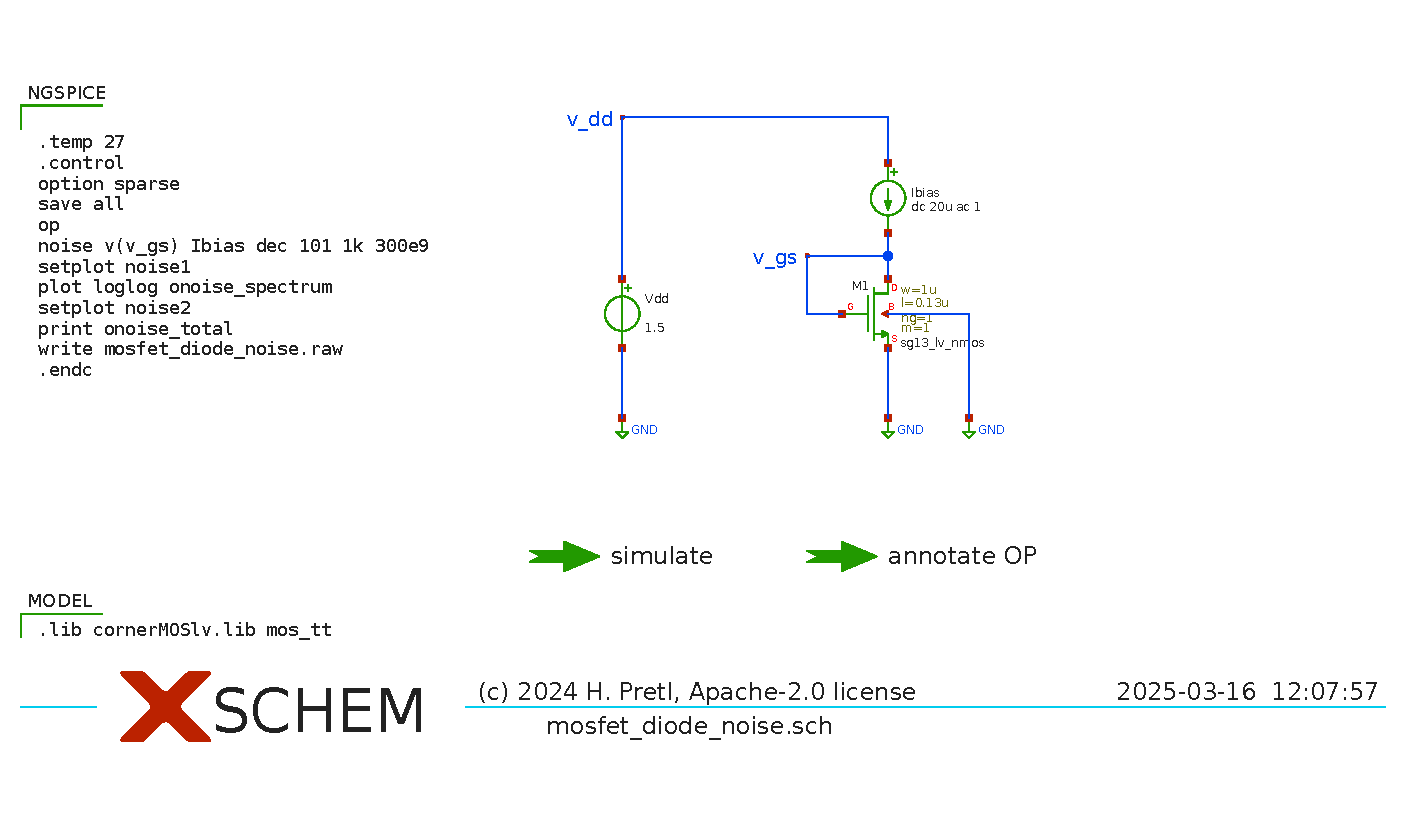
\includegraphics[keepaspectratio]{index_files/mediabag/xschem/mosfet_diode_noise.pdf}}

}

\caption{\label{fig-mosfet-diode-noise-tb}Testbench for MOSFET diode
noise analysis.}

\end{figure}%

\end{tcolorbox}

\subsection{Conclusion}\label{conclusion-1}

In this section we investigated the simple MOSFET-diode circuit. We
learned important skills like how to derive a small-signal model and how
to calculate important features like noise and open-loop gain for
stability analysis. We introduced Middlebrook's method to have a
mechanism to open up loops in simulation (and calculation) without
disturbing dc operating points or introduce errors by changing loading
conditions.

If you feel that you have not yet mastered these topics or are uncertain
in the operation of Xschem or ngspice, please go back to the beginning
of the section and read through the theory and redo the exercises.

\section{Common-Source Amplifier}\label{sec-cs-amplifier}

We now want to step up our game, and use more components to design
something useful. We will use a basic circuit structure, namely a
single-ended common-source amplifier. The structure of this circuit,
using a resistor as a load, is shown in Figure~\ref{fig-cs-amplifier}.

\textsubscript{Source:
\href{https://iic-jku.github.io/analog-circuit-design/index.qmd.html}{Article
Notebook}}

\begin{figure}[H]

\centering{

\pandocbounded{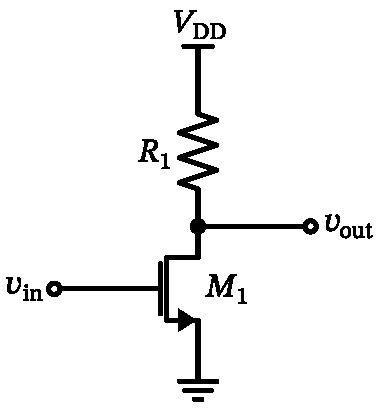
\includegraphics[keepaspectratio]{index_files/mediabag/index_files/figure-pdf/fig-cs-amplifier-output-1.pdf}}

}

\caption{\label{fig-cs-amplifier}A MOSFET common-source amplifier with
resistive load.}

\end{figure}%

\textsubscript{Source:
\href{https://iic-jku.github.io/analog-circuit-design/index.qmd.html}{Article
Notebook}}

The function of this circuit is as follows: Assuming the MOSFET \(M_1\)
is kept in saturation, then a small-signal voltage \(v_\mathrm{in}\)
applied at the gate is converted into a drain current \(i_\mathrm{d}\)
by the MOSFET's transconductance \(g_\mathrm{m}\). Then, this current is
converted into a voltage again in the resistor \(R_1\). Ultimately, we
have a dc voltage gain \(A_\mathrm{v}\) of

\[
A_\mathrm{v} = \frac{v_\mathrm{out}}{v_\mathrm{in}} \approx - \frac{g_\mathrm{m}v_\mathrm{in} R_1}{v_\mathrm{in}} = - g_\mathrm{m}R_1.
\]

As explained above, it is a good approach to see electronic circuit
components as

\begin{itemize}
\tightlist
\item
  voltage-to-current (MOSFET as common-source or common-gate; resistor),
\item
  current-to-voltage (resistor),
\item
  current-to-current (MOSFET as common-gate), and
\item
  voltage-to-voltage (MOSFET as common-drain)
\end{itemize}

conversions for better understanding.

\subsection{Sense Amplifier Driving 50 Ohm Matched
Load}\label{sense-amplifier-driving-50-ohm-matched-load}

Let us now size and design an exemplary implementation of this amplifier
(of course using the \(g_\mathrm{m}/I_\mathrm{D}\) method). In order to
have useful real-life specifications, we want to build an amplifier
which can be used to sense an on-chip voltage and drive off-chip
measurement equipment. Often, this equipment has an input impedance of
50\(\Omega\), and we want to have an impedance-matched output. The
voltage gain shall be set to 1 (essentially, we want to sense a voltage
and drive the measurement equipment).

The resulting circuit is shown in Figure~\ref{fig-meas-amplifier}. As
the load is usually ground-referred, and we want to avoid a dc-block at
the output, we use a PMOS amplifier stage (compare with
Figure~\ref{fig-cs-amplifier}).

\textsubscript{Source:
\href{https://iic-jku.github.io/analog-circuit-design/index.qmd.html}{Article
Notebook}}

\begin{figure}[H]

\centering{

\pandocbounded{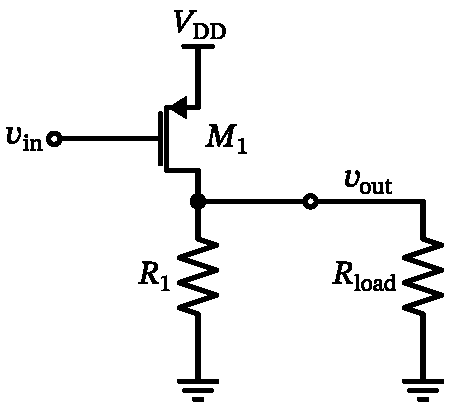
\includegraphics[keepaspectratio]{index_files/mediabag/index_files/figure-pdf/fig-meas-amplifier-output-1.pdf}}

}

\caption{\label{fig-meas-amplifier}A MOSFET common-source amplifier with
50 Ohm load.}

\end{figure}%

\textsubscript{Source:
\href{https://iic-jku.github.io/analog-circuit-design/index.qmd.html}{Article
Notebook}}

\begin{tcolorbox}[enhanced jigsaw, breakable, arc=.35mm, colbacktitle=quarto-callout-tip-color!10!white, toprule=.15mm, left=2mm, toptitle=1mm, bottomtitle=1mm, opacityback=0, rightrule=.15mm, opacitybacktitle=0.6, titlerule=0mm, colback=white, colframe=quarto-callout-tip-color-frame, coltitle=black, title=\textcolor{quarto-callout-tip-color}{\faLightbulb}\hspace{0.5em}{Exercise: PMOS-Based Measurement Amplifier}, bottomrule=.15mm, leftrule=.75mm]

Please think about why exactly we want this measurement amplifier be
based on a PMOS instead of an NMOS.

\end{tcolorbox}

The \href{https://en.wikipedia.org/wiki/Impedance_matching}{power
matching} requirement at the output mandates that
\(R_1 = R_\mathrm{load}\), so
\(R'_1 = R_\mathrm{load} \parallel R_1 = 25\,\Omega\). The voltage gain
requirement of \(|A_\mathrm{v}| = 1\) results in
\(g_\mathrm{m}= 1 / R'_1 = 40\,\text{mS}\).

We now need to find \(W\) and \(L\) of \(M_1\) and calculate the
required bias current \(I_\mathrm{D}\). We also need to find the proper
\(V_\mathrm{GS}\) to set this current. As usual, we use a Jupyter
notebook to calculate these values. Since we require modest speed of
this buffer we use a \(g_\mathrm{m}/I_\mathrm{D}=8\) and set
\(L = 0.13\,\mu\text{m}\). The notebook is available
\href{./sizing/sizing_measurement_amplifier.ipynb}{here}. The resulting
circuit including all component values is shown at the end of the
notebook (the red input capacitor shows the \(C_\mathrm{gg}\) of the
MOSFET).

\begin{tcolorbox}[enhanced jigsaw, breakable, arc=.35mm, colbacktitle=quarto-callout-important-color!10!white, toprule=.15mm, left=2mm, toptitle=1mm, bottomtitle=1mm, opacityback=0, rightrule=.15mm, opacitybacktitle=0.6, titlerule=0mm, colback=white, colframe=quarto-callout-important-color-frame, coltitle=black, title=\textcolor{quarto-callout-important-color}{\faExclamation}\hspace{0.5em}{Important \ref*{imp-mosfet-params-ng-m}: MOSFET Parameters NG and M}, bottomrule=.15mm, leftrule=.75mm]

\quartocalloutimp{imp-mosfet-params-ng-m} 

When sizing the MOSFET for this example we found that we need a fairly
large \(W\), resulting in a MOSFET aspect ratio of \(W/L \gg 1000\).
When constructing an integrated circuit out of individual MOSFET we
strive for an overall IC dimension that is roughly quadratic. For MOSFET
with large aspect ratios we need to get them into a comfortable shape.

In order to achieve this, we construct the MOSFET out of smaller pieces,
and the size of this pieces (called ``gate fingers'') are controlled by
the parameter \texttt{ng}. These MOSFET gate fingers all have the same
\(L\), but their width is \(W_\mathrm{finger} = W / \text{ng}\). All
this individual smaller MOSFET are connected in parallel.

In order to increase the MOSFET model accuracy, often the maximum value
of \(W_\mathrm{finger}\) is limited. In the case of SG13G2
\(W_\mathrm{finger} \le 10\,\mu\text{m}\).

In order to construct even larger MOSFET, we can connect multiple MOSFET
in parallel. We can do this in the circuit editor by placing and
connected these MOSFET; but since this is often used there is a more
convenient way: By using the parameter \texttt{m} (``multiplier'' or
``multiplicity'') we instantiate \(m\) MOSFET connected in parallel.

When to use \texttt{ng} and when to use \texttt{m}? The use of
\texttt{ng} results in a more compact IC layout, and is thus generally
preferable. Only in certain instances (e.g., when using a really large
\(W\)) \texttt{m} should be used. Further, the thoughtful use of
\texttt{ng} \textbf{allows to construct all the NMOS and PMOS of a
circuit out of the same gate finger elements}. This will result in a
very compact layout!

\end{tcolorbox}

\begin{tcolorbox}[enhanced jigsaw, breakable, arc=.35mm, colbacktitle=quarto-callout-tip-color!10!white, toprule=.15mm, left=2mm, toptitle=1mm, bottomtitle=1mm, opacityback=0, rightrule=.15mm, opacitybacktitle=0.6, titlerule=0mm, colback=white, colframe=quarto-callout-tip-color-frame, coltitle=black, title=\textcolor{quarto-callout-tip-color}{\faLightbulb}\hspace{0.5em}{Exercise: Measurement Amplifier Simulation}, bottomrule=.15mm, leftrule=.75mm]

Please go through the
\href{./sizing/sizing_measurement_amplifier.ipynb}{sizing notebook} of
the measurement amplifier and double-check the calculations. Do you
agree that the calculations are correct?

Once you agree with the circuit sizing please build an Xschem simulation
testbench where you simulate the small-signal voltage gain
\(A_\mathrm{v}\) of this measurement amplifier if it is driven with an
ideal voltage source. Keep in mind that the maximum MOSFET finger width
is 10µm in this technology, so you need to set the parameter \texttt{ng}
accordingly (see Important~\ref{imp-mosfet-params-ng-m}).

\begin{itemize}
\tightlist
\item
  What is the dc gain of this amplifier when loaded with 50\(\Omega\)?
\item
  The dc gain is likely not exactly 0dB. Why is this so?
\item
  Increase the width \(W\) of the PMOS until the gain is correct. What
  is the \(W\) that you had to set, and how much is \(I_\mathrm{D}\)
  now?
\item
  What is the bandwidth (i.e., the -3dB corner frequency) of the output
  voltage, when the voltage source has a source resistance of
  1k\(\Omega\)?
\end{itemize}

If you get stuck, \href{./xschem/measurement_amplifier.sch}{here} is the
solution to this exercise, and it is also shown in
Figure~\ref{fig-meas-amp-tb}.

\begin{figure}[H]

\centering{

\pandocbounded{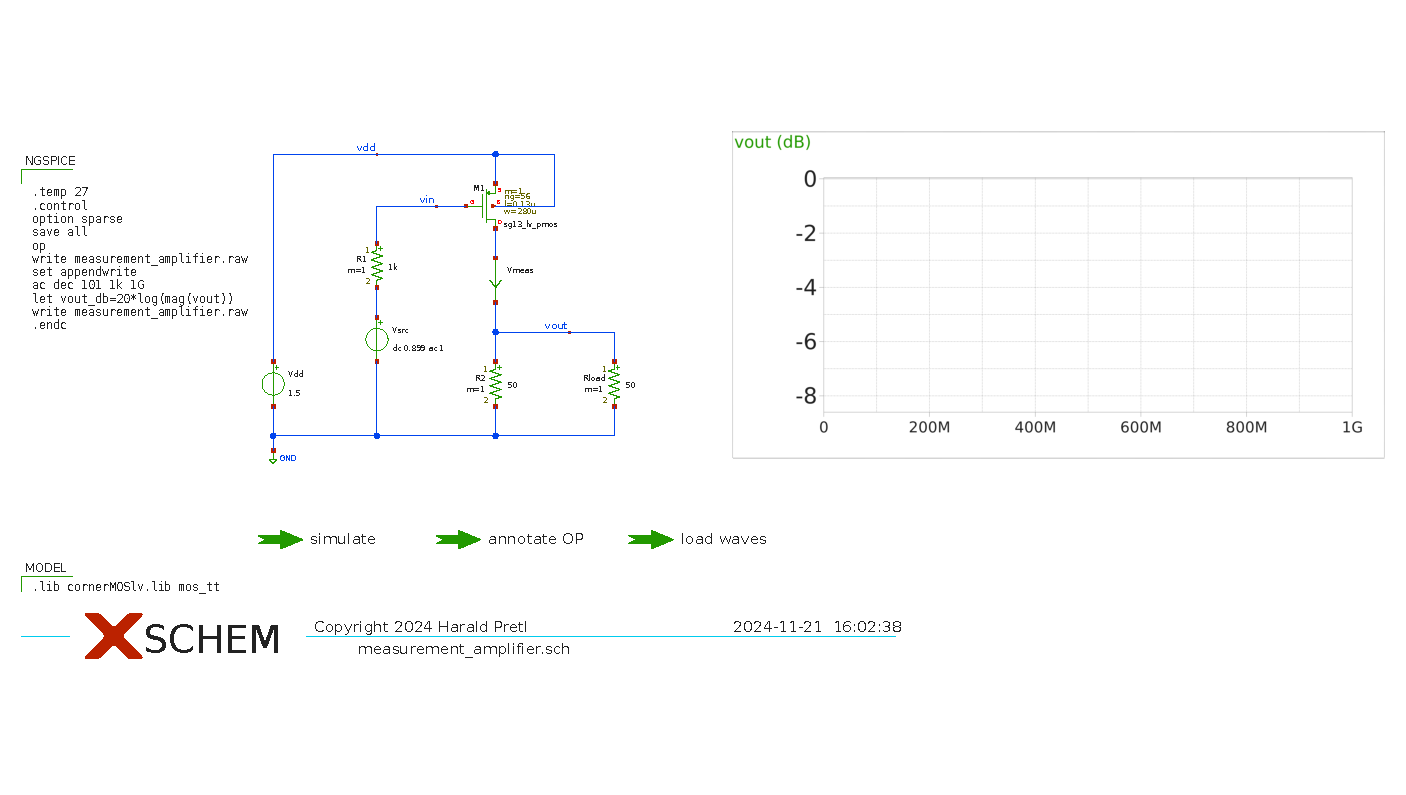
\includegraphics[keepaspectratio]{index_files/mediabag/xschem/measurement_amplifier.pdf}}

}

\caption{\label{fig-meas-amp-tb}Simulation schematic of the
common-source measurement amplifier.}

\end{figure}%

\end{tcolorbox}

By now we have designed a measurement amplifier based on a common-source
stage. One problem with this stage is the relatively large input
capacitance \(C_\mathrm{GG}\) of approx. 0.3pF, which loads the input
source. Another issue even more severe is that the fact that the bias
point in this circuit is set by the dc voltage level at the input. In
general, we want a setup where the bias points of the circuit are
largely independent of the dc input voltages. This is why in integrated
circuit design we often design \textbf{differential circuits} where the
input and output signals are given by the differential voltages, and are
largely independent from the common-mode voltages. This is usually an
advantage.

\section{Current Mirror}\label{sec-current-mirror}

In this section we will look into a fundamental building block which is
often used in integrated circuit design, the \textbf{current mirror} (R.
Widlar 1965). A diagram is shown in Figure~\ref{fig-current-mirror} with
one MOSFET diode converting the incoming bias current into a voltage
\(V_\mathrm{GS}= f(I_\mathrm{D1}) = f(I_\mathrm{bias})\), and two output
MOSFETs working as current sources, which are biased from the diode. By
properly selecting all \(W\) and \(L\) the input current can be scaled,
and multiple copies can be created at once. Shown in the figure are two
output currents \(I_\mathrm{out1}\) and \(I_\mathrm{out2}\), but any
number of parallel branches can be realized (note that this is true for
MOSFET as no gate current flows; for the case of BJTs, the base current
flowing into the various transistors is subtracted from
\(I_\mathrm{bias}\), so usually a compensation circuit is added).

\textsubscript{Source:
\href{https://iic-jku.github.io/analog-circuit-design/index.qmd.html}{Article
Notebook}}

\begin{figure}[H]

\centering{

\pandocbounded{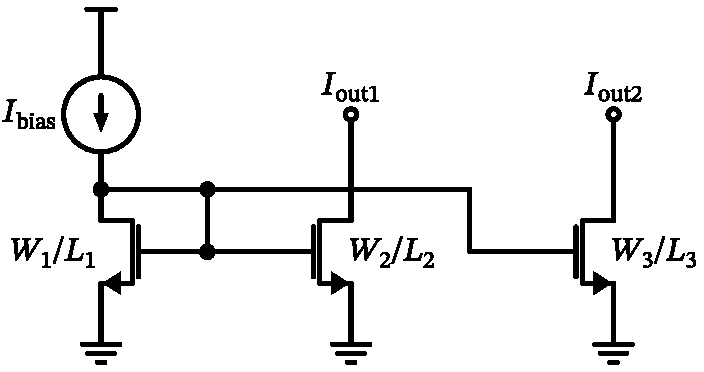
\includegraphics[keepaspectratio]{index_files/mediabag/index_files/figure-pdf/fig-current-mirror-output-1.pdf}}

}

\caption{\label{fig-current-mirror}A current mirror with two output
branches.}

\end{figure}%

\textsubscript{Source:
\href{https://iic-jku.github.io/analog-circuit-design/index.qmd.html}{Article
Notebook}}

Neglecting the impact of \(g_\mathrm{ds1}\) and \(g_\mathrm{ds2}\), the
output current \(I_\mathrm{out1}\) is then given by \[
I_\mathrm{out1} \approx I_\mathrm{bias} \frac{W_2}{L_2} \frac{L_1}{W_1}
\] and the output current \(I_\mathrm{out2}\) is given by \[
I_\mathrm{out2} \approx I_\mathrm{bias} \frac{W_3}{L_3} \frac{L_1}{W_1}.
\]

For good matching care has to be taken that the MOSFET widths and
lengths are constructed out of \textbf{unit elements} of identical size,
where an appropriate amount of these single units are then arranged in
series or parallel configuration to arrive at the target \(W\) and \(L\)
(remember MOSFET parameters \texttt{ng} and \texttt{m}, see
Important~\ref{imp-mosfet-params-ng-m}).

As we know from earlier investigations of the MOSFET performance in
Section~\ref{sec-gmid-method} the drain current of a MOSFET is a
function of \(V_\mathrm{GS}\) and \(V_\mathrm{DS}\). As long as the
MOSFET stays in saturation (i.e., \(V_\mathrm{DS}> V_\mathrm{ds,dsat}\))
the drain current is just a mild function of \(V_\mathrm{DS}\)
(essentially the effect of \(g_\mathrm{ds}\), which is the output
conductance of the MOSFET). A fundamental flaw/limitation of the basic
current mirror shown in Figure~\ref{fig-current-mirror} is the mismatch
of the \(V_\mathrm{DS}\) of the MOSFETs. The input-side diode has
\(V_\mathrm{GS}= V_\mathrm{DS1}\), whereas the output current sources
have a \(V_\mathrm{DS2,3}\) depending on the connected circuitry.
Improved current mirrors exist (fixing this flaw), however, when a
current mirror is required with mediocre performance requirements this
structure can be used for its simplicity.

\begin{tcolorbox}[enhanced jigsaw, breakable, arc=.35mm, colbacktitle=quarto-callout-tip-color!10!white, toprule=.15mm, left=2mm, toptitle=1mm, bottomtitle=1mm, opacityback=0, rightrule=.15mm, opacitybacktitle=0.6, titlerule=0mm, colback=white, colframe=quarto-callout-tip-color-frame, coltitle=black, title=\textcolor{quarto-callout-tip-color}{\faLightbulb}\hspace{0.5em}{Exercise: Current Mirror}, bottomrule=.15mm, leftrule=.75mm]

Please construct a current mirror based on the MOSFET-diode which we
sized in Section~\ref{sec-mosfet-diode}. The input current
\(I_\mathrm{bias} = 20\,\mu\text{A}\), and we want three output currents
of size \(10\,\mu\text{A}\), \(20\,\mu\text{A}\), and
\(40\,\mu\text{A}\).

Sweep the output voltage of all three current branches and see over
which voltage range an acceptable current is created. For which output
voltage range is the current departing from its ideal value, and why?

You see that the slope of the output current is quite bad, as
\(g_\mathrm{ds}\) is too large. We can improve this by changing the
length to \(L = 5\,\mu\text{m}\) (for motivation, please look at the
graphs in Section~\ref{sec-gmid-method}). In addition, for a current
mirror we are not interested in a high \(g_\mathrm{m}/I_\mathrm{D}\)
value, so we can use \(g_\mathrm{m}/I_\mathrm{D}= 5\) in this case.
Please size the current mirror MOSFETs accordingly (please round the
\(W\) to half micron, to keep sizes a bit more practical). Compare this
result to the previous one, what changed?

In case you get stuck, here are Xschem schematics for the
\href{./xschem/current_mirror.sch}{original} and the
\href{./xschem/current_mirror_improved.sch}{improved} current mirrors.

\end{tcolorbox}

\section{Differential Pair}\label{sec-diff-pair}

Like the current mirror in Section~\ref{sec-current-mirror} the
\textbf{differential pair} is an ubiquitous building block often used in
integrated circuit design (Blumlein 1937). The fundamental structure is
given in Figure~\ref{fig-differential-pair}.

\textsubscript{Source:
\href{https://iic-jku.github.io/analog-circuit-design/index.qmd.html}{Article
Notebook}}

\begin{figure}[H]

\centering{

\pandocbounded{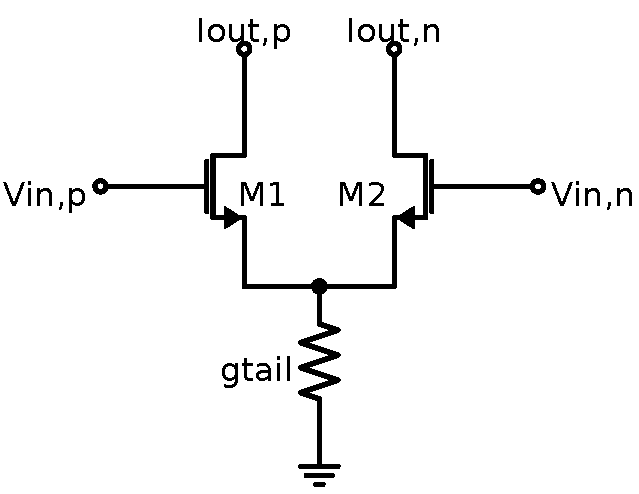
\includegraphics[keepaspectratio]{index_files/mediabag/index_files/figure-pdf/fig-differential-pair-output-1.pdf}}

}

\caption{\label{fig-differential-pair}A differential pair.}

\end{figure}%

\textsubscript{Source:
\href{https://iic-jku.github.io/analog-circuit-design/index.qmd.html}{Article
Notebook}}

In order to understand its operation it is instructive to separate the
input condition into (1) a purely differential voltage, and (2) a
common-mode voltage, and see what the impact on the output currents is.

\subsection{Differential Operation of the
Diffpair}\label{differential-operation-of-the-diffpair}

For a differential mode of operation we assume that the input common
mode voltage is constant, i.e.,
\((V_\mathrm{in,p} + V_\mathrm{in,n})/2 = V_\mathrm{CM}\). The
differential input voltage
\(v_\mathrm{in} = V_\mathrm{in,p} - V_\mathrm{in,n}\), so that \[
V_\mathrm{in,p} = V_\mathrm{CM} + \frac{v_\mathrm{in}}{2}
\] and \[
V_\mathrm{in,n} = V_\mathrm{CM} - \frac{v_\mathrm{in}}{2}.
\]

For a small-signal differential drive the potential at the tail point
stays constant and we can treat it as a virtual ground. The output
current on each side is then given by (neglecting \(g_\mathrm{ds}\) and
\(g_\mathrm{mb}\) of \(M_1\) and \(M_2\)) \[
i_\mathrm{out,p} = g_\mathrm{m1} \left( \frac{v_\mathrm{in}}{2} \right)
\] and \[
i_\mathrm{out,n} = g_\mathrm{m2} \left( -\frac{v_\mathrm{in}}{2} \right).
\]

Usually we assume symmetry in the differential pair, so
\(g_\mathrm{m1} = g_\mathrm{m2} = g_\mathrm{m}\). The differential
output current \(i_\mathrm{out}\) is then given by
\begin{equation}\phantomsection\label{eq-differential-pair-dm}{
i_\mathrm{out} = i_\mathrm{out,p} - i_\mathrm{out,n} = g_\mathrm{m}v_\mathrm{in}
}\end{equation}

We see in Equation~\ref{eq-differential-pair-dm} that the differential
output current is simply the differential input voltage multiplied by
the \(g_\mathrm{m}\) of the individual transistor. We also note that the
bottom conductance \(g_\mathrm{tail}\) plays no role for the
small-signal differential operation.

\subsection{Common-Mode Operation of the
Diffpair}\label{common-mode-operation-of-the-diffpair}

Usually, the source conductance \(g_\mathrm{tail}\) is realized by a
current source and ideally should be \(g_\mathrm{tail} = 0\). If this is
the case, then the output currents are not a function of the common-mode
input voltage (\(I_\mathrm{tail}\) is set by the tail current source),
and \[
I_\mathrm{out,p} = I_\mathrm{out,n} = \frac{I_\mathrm{tail}}{2}.
\]

However, if we assume a realistic tail current source then
\(g_\mathrm{tail} > 0\). For analysis we can simply look at a half
circuit since the circuit operation is symmetric. In order to simplify
the analysis a bit we remove all capacitors from the MOSFET small-signal
model and set \(g_\mathrm{ds}= g_\mathrm{mb}= 0\). We then arrive at the
small-signal equivalent circuit shown in
Figure~\ref{fig-differential-pair-cm} (note that we set
\(v_\mathrm{in,p} = v_\mathrm{in,n} = v_\mathrm{in}\) and
\(i_\mathrm{out,p} = i_\mathrm{out,n} = i_\mathrm{out}\) under symmetry
considerations).

\textsubscript{Source:
\href{https://iic-jku.github.io/analog-circuit-design/index.qmd.html}{Article
Notebook}}

\begin{figure}[H]

\centering{

\pandocbounded{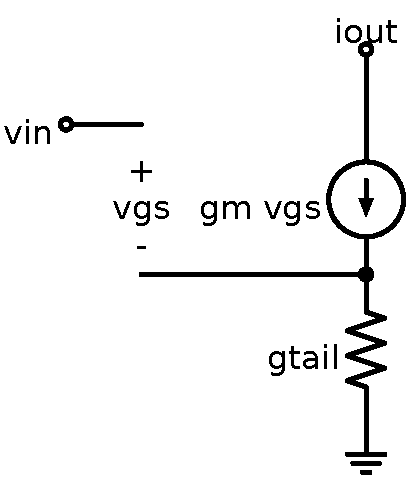
\includegraphics[keepaspectratio]{index_files/mediabag/index_files/figure-pdf/fig-differential-pair-cm-output-1.pdf}}

}

\caption{\label{fig-differential-pair-cm}Small-signal model of the
differential pair half-circuit in common-mode operation.}

\end{figure}%

\textsubscript{Source:
\href{https://iic-jku.github.io/analog-circuit-design/index.qmd.html}{Article
Notebook}}

Formulating KVL for the input-side loop we get \[
v_\mathrm{in} = v_\mathrm{gs}+ \frac{i_\mathrm{d}}{g_\mathrm{tail}}.
\]

With \(i_\mathrm{out} = i_\mathrm{d}= g_\mathrm{m}v_\mathrm{gs}\) we
arrive at
\begin{equation}\phantomsection\label{eq-differential-pair-cm}{
i_\mathrm{out} = \frac{g_\mathrm{m}g_\mathrm{tail}}{g_\mathrm{m}+ g_\mathrm{tail}} v_\mathrm{in}
}\end{equation}

Interpreting Equation~\ref{eq-differential-pair-cm} we can distinguish
the following extreme cases:

\begin{enumerate}
\def\labelenumi{\arabic{enumi}.}
\tightlist
\item
  If \(g_\mathrm{tail} = 0\) (ideal tail current source) then
  \(i_\mathrm{out} = 0\), the common-mode voltage variation from the
  input is suppressed and does not show up at the common-mode output
  current (which is constant due to the ideal tail current source). This
  is usually the case that we want to achieve.
\item
  If \(g_\mathrm{tail} \rightarrow \infty\) then
  \(i_\mathrm{out} = g_\mathrm{m}v_\mathrm{in}\), which means the output
  current is a function of the MOSFET \(g_\mathrm{m}\). If everything is
  perfectly matched, then the differential output current is zero, but
  the common-mode output current changes according to the common-mode
  input voltage. In special cases this can be a wanted behavior, this
  configuration is called a ``pseudo-differential pair.''
\end{enumerate}

Note that the result of Equation~\ref{eq-differential-pair-cm} is also
valid for the general case of a degenerated common-source transistor
stage (see Figure~\ref{fig-common-source-degenerated}). The effective
transconductange \(g_\mathrm{m}'\) is given by
(\(R_\mathrm{degen} = g_\mathrm{tail}^{-1}\))

\[
g_\mathrm{m}' = \frac{i_\mathrm{out}}{v_\mathrm{in}} = \frac{g_\mathrm{m}g_\mathrm{tail}}{g_\mathrm{m}+ g_\mathrm{tail}} = \frac{1}{g_\mathrm{m}^{-1} + R_\mathrm{degen}}.
\]

When no degeneration resistor is used, then
\(g_\mathrm{m}' = g_\mathrm{m}\). If a degeneration of
\(R_\mathrm{degen} \gg g_\mathrm{m}^{-1}\) is used then
\(g_\mathrm{m}' = 1 / R_\mathrm{degen}\). This result is worth
memorizing.

\textsubscript{Source:
\href{https://iic-jku.github.io/analog-circuit-design/index.qmd.html}{Article
Notebook}}

\begin{figure}[H]

\centering{

\pandocbounded{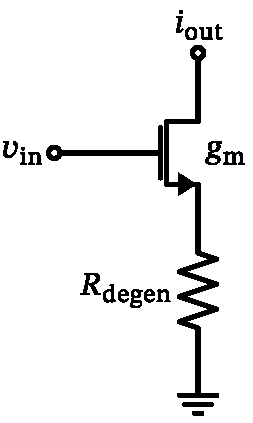
\includegraphics[keepaspectratio]{index_files/mediabag/index_files/figure-pdf/fig-common-source-degenerated-output-1.pdf}}

}

\caption{\label{fig-common-source-degenerated}A MOSFET common-source
amplifier with resistive degeneration.}

\end{figure}%

\textsubscript{Source:
\href{https://iic-jku.github.io/analog-circuit-design/index.qmd.html}{Article
Notebook}}

\section{A Basic 5-Transistor OTA}\label{sec-basic-ota}

Suited with the insights of basic transistor operation
(Section~\ref{sec-first-steps} and Section~\ref{sec-gmid-method}) and
the working knowledge of the current mirror
(Section~\ref{sec-mosfet-diode} and Section~\ref{sec-current-mirror}) as
well as the differential pair (Section~\ref{sec-diff-pair}) we can now
start to design our first real circuit. A fundamental (simple) circuit
that is often used for basic tasks is the 5-transistor operational
transconductance amplifier (OTA). A circuit diagram of this 5T-OTA is
shown in Figure~\ref{fig-basic-ota}.

\textsubscript{Source:
\href{https://iic-jku.github.io/analog-circuit-design/index.qmd.html}{Article
Notebook}}

\begin{figure}[H]

\centering{

\pandocbounded{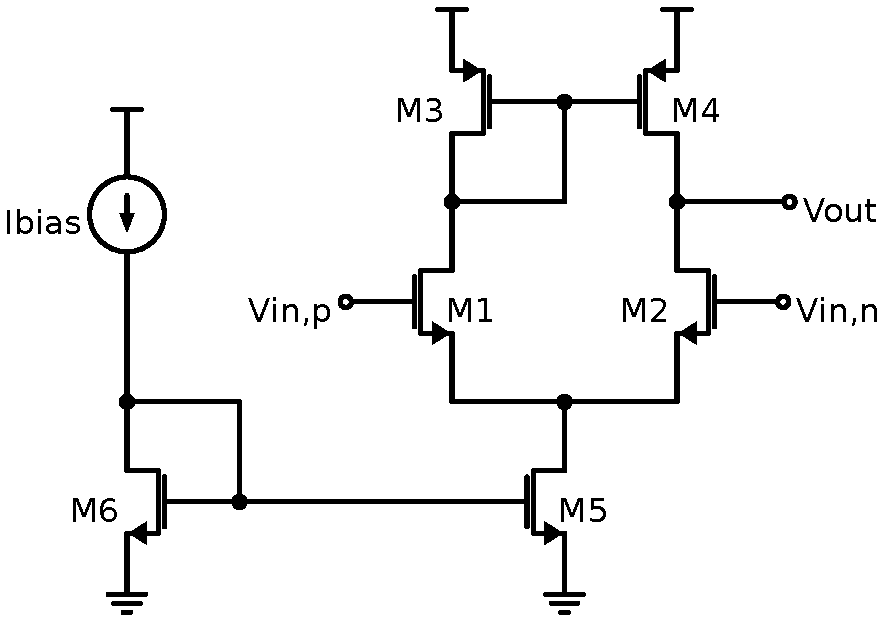
\includegraphics[keepaspectratio]{index_files/mediabag/index_files/figure-pdf/fig-basic-ota-output-1.pdf}}

}

\caption{\label{fig-basic-ota}The 5-transistor OTA.}

\end{figure}%

\textsubscript{Source:
\href{https://iic-jku.github.io/analog-circuit-design/index.qmd.html}{Article
Notebook}}

\begin{tcolorbox}[enhanced jigsaw, breakable, arc=.35mm, colbacktitle=quarto-callout-warning-color!10!white, toprule=.15mm, left=2mm, toptitle=1mm, bottomtitle=1mm, opacityback=0, rightrule=.15mm, opacitybacktitle=0.6, titlerule=0mm, colback=white, colframe=quarto-callout-warning-color-frame, coltitle=black, title=\textcolor{quarto-callout-warning-color}{\faExclamationTriangle}\hspace{0.5em}{Refresh MOSFET Basic Circuits}, bottomrule=.15mm, leftrule=.75mm]

While we repeat the basics of elementary MOSFET amplifier stages (like
common-source stage, common-gate stage, and current mirror) in this
course material, the following compendium (Murmann 2013) is recommended
for review. It is freely available at
\url{https://github.com/bmurmann/Book-on-MOS-stages}.

In addition, we can highly recommend these references Razavi (2017) for
further study.

\end{tcolorbox}

The operation is as follows: \(M_{1,2}\) form a differential pair which
is biased by the current source \(M_5\). \(M_{5,6}\) form a current
mirror, thus the input bias current \(I_\mathrm{bias}\) sets the bias
current in the OTA. The differential pair \(M_{1,2}\) is loaded by the
current mirror \(M_{3,4}\) which mirrors the drain current of \(M_1\) to
the right side. Here, the currents from \(M_4\) and \(M_2\) are summed,
and together with the conductance effective at the output node a voltage
builds up.

\begin{tcolorbox}[enhanced jigsaw, breakable, arc=.35mm, colbacktitle=quarto-callout-note-color!10!white, toprule=.15mm, left=2mm, toptitle=1mm, bottomtitle=1mm, opacityback=0, rightrule=.15mm, opacitybacktitle=0.6, titlerule=0mm, colback=white, colframe=quarto-callout-note-color-frame, coltitle=black, title=\textcolor{quarto-callout-note-color}{\faInfo}\hspace{0.5em}{Operational Amplifier (op-amp, OPA) vs.~Operational Transconductance
Amplifier (OTA)}, bottomrule=.15mm, leftrule=.75mm]

An
\href{https://en.wikipedia.org/wiki/Operational_amplifier}{operational
amplifier} is a universal electronic building block characterized by (in
the ideal case):

\begin{itemize}
\tightlist
\item
  infinite input impedance at the input ports
  (\(R_\mathrm{in} \rightarrow \infty\))
\item
  zero output resistance, i.e., a voltage output
  (\(R_\mathrm{out} = 0\))
\item
  infinite voltage gain
  (\(A_\mathrm{v} = V_\mathrm{out} / V_\mathrm{in} \rightarrow \infty\))
\end{itemize}

An
\href{https://en.wikipedia.org/wiki/Operational_transconductance_amplifier}{operational
transconductance amplifier} is a building block characterized by (again
in the ideal case):

\begin{itemize}
\tightlist
\item
  infinite input impedance at the input ports
  (\(R_\mathrm{in} \rightarrow \infty\))
\item
  infinite output resistance, i.e., a current output
  (\(R_\mathrm{out} \rightarrow \infty\))
\item
  infinite transconductance
  (\(G = I_\mathrm{out} / V_\mathrm{in} \rightarrow \infty\))
\end{itemize}

In integrated circuits, we very often load an OPA/OTA high-ohmic, i.e.,
with a capacitive load. Hence, an OTA can be used to create a
voltage-mode amplifier with high gain, approaching the properties of the
OPA. If an OTA is used to drive a low-ohmic load, the voltage gain will
be low, and we have to use this block as a transconductance amplifier.
Since the output changes behavior depending on high- or low-ohmic
loading, we label the output in Figure~\ref{fig-basic-ota} accordingly.

Why then implement an OTA instead of an OPA? Usually, an OTA is a
simpler structure than an OPA. As a general rule, the simplest circuit
that can do a job is usually the best choice.

\end{tcolorbox}

We note that \(M_{1,2}\) and \(M_{3,4}\) need to be symmetric, thus will
have the same \(W\) and \(L\) dimensioning. \(M_{5,6}\) we scale
accordingly to set the correct bias current in the OTA.

\subsection{Voltage Buffer with OTA}\label{sec-voltage-buffer-with-ota}

In order to design an OTA we need an application, and from this we need
to derive the circuit specifications. We want to use this OTA to realize
a voltage buffer which lightly loads an input voltage source and can
drive a large capacitive load. Such a configuration is often used to,
e.g., buffer a reference voltage that is needed (and thus loaded) by
another circuit. The block diagram of this configuration is shown in
Figure~\ref{fig-voltage-buffer-ota}.

\textsubscript{Source:
\href{https://iic-jku.github.io/analog-circuit-design/index.qmd.html}{Article
Notebook}}

\begin{figure}[H]

\centering{

\pandocbounded{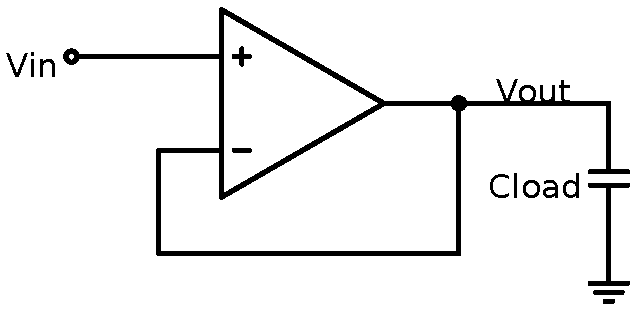
\includegraphics[keepaspectratio]{index_files/mediabag/index_files/figure-pdf/fig-voltage-buffer-ota-output-1.pdf}}

}

\caption{\label{fig-voltage-buffer-ota}A voltage buffer (based on OTA)
driving a capacitive load.}

\end{figure}%

\textsubscript{Source:
\href{https://iic-jku.github.io/analog-circuit-design/index.qmd.html}{Article
Notebook}}

If the voltage gain of the OTA in Figure~\ref{fig-voltage-buffer-ota} is
high, then \(V_\mathrm{out} \approx V_\mathrm{in}\). We now want to
design an OTA for this application fitting the following specification
values (see Table~\ref{tbl-voltage-buffer-spec}). These values are
rather typical of what could be expected for such a buffer design.

\begin{longtable}[]{@{}
  >{\raggedright\arraybackslash}p{(\linewidth - 4\tabcolsep) * \real{0.5588}}
  >{\centering\arraybackslash}p{(\linewidth - 4\tabcolsep) * \real{0.3529}}
  >{\centering\arraybackslash}p{(\linewidth - 4\tabcolsep) * \real{0.0882}}@{}}
\caption{Voltage buffer
specification}\label{tbl-voltage-buffer-spec}\tabularnewline
\toprule\noalign{}
\begin{minipage}[b]{\linewidth}\raggedright
Specification
\end{minipage} & \begin{minipage}[b]{\linewidth}\centering
Value
\end{minipage} & \begin{minipage}[b]{\linewidth}\centering
Unit
\end{minipage} \\
\midrule\noalign{}
\endfirsthead
\toprule\noalign{}
\begin{minipage}[b]{\linewidth}\raggedright
Specification
\end{minipage} & \begin{minipage}[b]{\linewidth}\centering
Value
\end{minipage} & \begin{minipage}[b]{\linewidth}\centering
Unit
\end{minipage} \\
\midrule\noalign{}
\endhead
\bottomrule\noalign{}
\endlastfoot
Supply voltage & \(1.45 < \underline{1.5} < 1.55\) & V \\
Temperature range (industrial) & \(-40 < \underline{27} < 125\) &
degC \\
Load capacitance \(C_\mathrm{load}\) & \(50\) & fF \\
Input voltage range (for buffering 2/3 bandgap voltage) &
\(0.7 < \underline{0.8} < 0.9\) & V \\
Signal bandwidth (3dB) & \(>10\) & MHz \\
Output voltage error & \(<3\) & \% \\
Total output noise (rms) & \(<1\) & mV\textsubscript{rms} \\
Supply current (as low as possible) & \(<10\) & µA \\
Stability & stable for rated \(C_\mathrm{load}\) & \\
Turn-on time (settled to with 1\%) & \(<10\) & µs \\
Externally provided bias current (nominal) & \(20\) & µA \\
\end{longtable}

\subsection{Large-Signal Analysis of the
OTA}\label{sec-basic-ota-large-signal}

The first step when receiving a design task is to look at the
specifications, and see whether they make sense. The detailed
performance of the design will be the result of the circuit simulation,
but before we step into sizing we need to do a few simple calculations
to (a) do back-of-the-envelope gauging if the specification makes sense,
and (b) use the derived analytical equations as guide for the sizing
procedure.

In terms of large-signal operation, we will now check whether the input
and output voltage range, as well as the settling time can be roughly
met. Since we do not know yet the resulting \(V_\mathrm{GS}\) of the
transistors we use \(0.6\,\text{V}\) as an initial guess. If we run into
issues with that guess we know how to later steer the sizing procedure.

\begin{itemize}
\tightlist
\item
  When the input is at its maximum of \(0.9\,\text{V}\), we see that we
  need to keep \(M_1\) in saturation. We can calculate that
  \(V_\mathrm{DS1} = V_\mathrm{DD}- |V_\mathrm{GS3}| + V_\mathrm{GS1} - V_\mathrm{in} = 1.45 - 0.6 + 0.6 - 0.9 = 0.55\,\text{V}\),
  which leaves enough margin.
\item
  When the input is at its minimum of \(0.7\,\text{V}\), we see that the
  \(V_\mathrm{DS5}\) of \(M_5\) is calculated as
  \(V_\mathrm{DS5} = V_\mathrm{in} - V_\mathrm{GS1} = 0.7 - 0.6 = 0.1\,\text{V}\),
  so this leaves little margin, but we can make \(V_\mathrm{GS1}\)
  smaller, so it should work out.
\item
  For the output voltage, when the output voltage is on the high side,
  it leaves
  \(|V_\mathrm{DS4}| = V_\mathrm{DD}- V_\mathrm{out} = 1.45 - 0.9 = 0.55\,\text{V}\),
  which is enough margin.
\end{itemize}

In summary, we think that we can make an NMOS-input OTA like the one in
Figure~\ref{fig-basic-ota} work for the required supply and input- and
output-voltages. If this would not work out, we need to look for further
options, like a PMOS-input OTA, or a NMOS/PMOS-input OTA.

Another large-signal specification item that we can quickly check is the
settling time. Under slewing conditions, the complete bias current in
the OTA is steered towards the output (try to understand why this is the
case), so when the output capacitor is fully discharged, and we assume
just a linear ramp due to constant-current charging of the output
capacitor, the settling time is \[
T_\mathrm{slew} \approx \frac{C_\mathrm{load} V_\mathrm{out}}{I_\mathrm{tail}} = \frac{50 \cdot 10^{-15} \cdot 1.3}{10 \cdot 10^{-6}} = 6.5\,\text{ns}
\] so this leaves plenty of margin for additional slow-signal settling
due to the limited bandwidth, as well as reducing the supply current.

The small-signal settling (assuming one pole at the bandwidth corner
frequency) leads to an approximate settling time (1\% error corresponds
to \(\approx 5 \tau\)) of \[
T_\mathrm{settle} \approx \frac{5}{2 \pi f_\mathrm{c}} = \frac{5}{2 \pi \cdot 1 \cdot 10^{6}} = 0.8\,\mu\text{s}.
\] which also checks out.

\subsection{Small-Signal Analysis of the
OTA}\label{sec-basic-ota-small-signal}

In order to size the OTA components we need to derive how the MOSFET
parameters define the performance. The important small-signal metrics
are

\begin{itemize}
\tightlist
\item
  dc voltage gain \(A_0\)
\item
  gain-bandwidth product (GBW)
\item
  output noise
\end{itemize}

The specification for GBW is directly given in
Table~\ref{tbl-voltage-buffer-spec}, while the dc gain we have to
calculate from the voltage accuracy specification. For a voltage
follower in the configuration shown in
Figure~\ref{fig-voltage-buffer-ota} the voltage gain is given by
\begin{equation}\phantomsection\label{eq-voltage-buffer-tolerance}{
\frac{V_\mathrm{out}}{V_\mathrm{in}} = \frac{A_0}{1 + A_0}.
}\end{equation}

So in order to reach an output voltage accuracy of at least 3\% we need
a dc gain of \(A_0 > 30.2\,\text{dB}\). To allow for process and
temperature variation we need to add a bit of extra gain as margin.

\begin{tcolorbox}[enhanced jigsaw, breakable, arc=.35mm, colbacktitle=quarto-callout-important-color!10!white, toprule=.15mm, left=2mm, toptitle=1mm, bottomtitle=1mm, opacityback=0, rightrule=.15mm, opacitybacktitle=0.6, titlerule=0mm, colback=white, colframe=quarto-callout-important-color-frame, coltitle=black, title=\textcolor{quarto-callout-important-color}{\faExclamation}\hspace{0.5em}{Small-Signal vs.~Large-Signal Operation}, bottomrule=.15mm, leftrule=.75mm]

In order to get the correct dc voltage per the specification we require
the large-signal gain calculated with
Equation~\ref{eq-voltage-buffer-tolerance}. However, calculating the
large-signal gain of a circuit is quite involved (usually mandating the
use of a large-signal nonlinear model for the used components), so we
typically resort to do a simpler small-signal calculation instead, like
in Section~\ref{sec-basic-ota-small-signal}. We deliberately introduce
this error, but we should not get confused about the difference between
large- and small-signal operation!

\end{tcolorbox}

\subsubsection{OTA Small-Signal Transfer
Function}\label{ota-small-signal-transfer-function}

In order to derive the governing small-signal equations for the OTA we
will make a few simplifications:

\begin{itemize}
\tightlist
\item
  We will set \(g_\mathrm{mb}= 0\) for all MOSFETs.
\item
  We will further set \(C_\mathrm{gd}= 0\) for all MOSFETs except for
  \(M_4\) where we expect a Miller effect on this capacitor, and we
  could add its effect by increasing the capacitance at the gate node of
  \(M_{3,4}\) (for background please see
  Section~\ref{sec-miller-theorem}). However, as this does not create a
  dominant pole in this circuit, we consider this a minor effect (see
  Equation~\ref{eq-simple-ota-gain}). Thus, only \(C_\mathrm{gs34}\) is
  considered at the gate node of the current mirror load.
\item
  We assume \(g_\mathrm{m}\gg g_\mathrm{ds}\), so we set
  \(g_\mathrm{ds1} = g_\mathrm{ds3} = 0\).
\item
  The drain capacitance of \(M_2\) and \(M_4\), as well as the gate
  capacitance of \(M_2\) we can add to the load capacitance
  \(C_\mathrm{load}\). Note that \(C_\mathrm{gs2}\) can be added because
  of the feedback connection between the inverting input and the output.
  However, this is not shown in the small-signal equivalent circuits
  below, because we are interested in the open-loop transfer function.
\end{itemize}

The resulting small-signal equivalent circuit is shown in
Figure~\ref{fig-basic-ota-small-signal}.

\begin{tcolorbox}[enhanced jigsaw, breakable, arc=.35mm, colbacktitle=quarto-callout-warning-color!10!white, toprule=.15mm, left=2mm, toptitle=1mm, bottomtitle=1mm, opacityback=0, rightrule=.15mm, opacitybacktitle=0.6, titlerule=0mm, colback=white, colframe=quarto-callout-warning-color-frame, coltitle=black, title=\textcolor{quarto-callout-warning-color}{\faExclamationTriangle}\hspace{0.5em}{Refresh MOSFET Small-Signal Model}, bottomrule=.15mm, leftrule=.75mm]

Please review the MOSFET small-signal equivalent model in
Figure~\ref{fig-mosfet-small-signal-model} at this point. For the PMOS
just flip the model upside-down.

\end{tcolorbox}

\textsubscript{Source:
\href{https://iic-jku.github.io/analog-circuit-design/index.qmd.html}{Article
Notebook}}

\begin{figure}[H]

\centering{

\pandocbounded{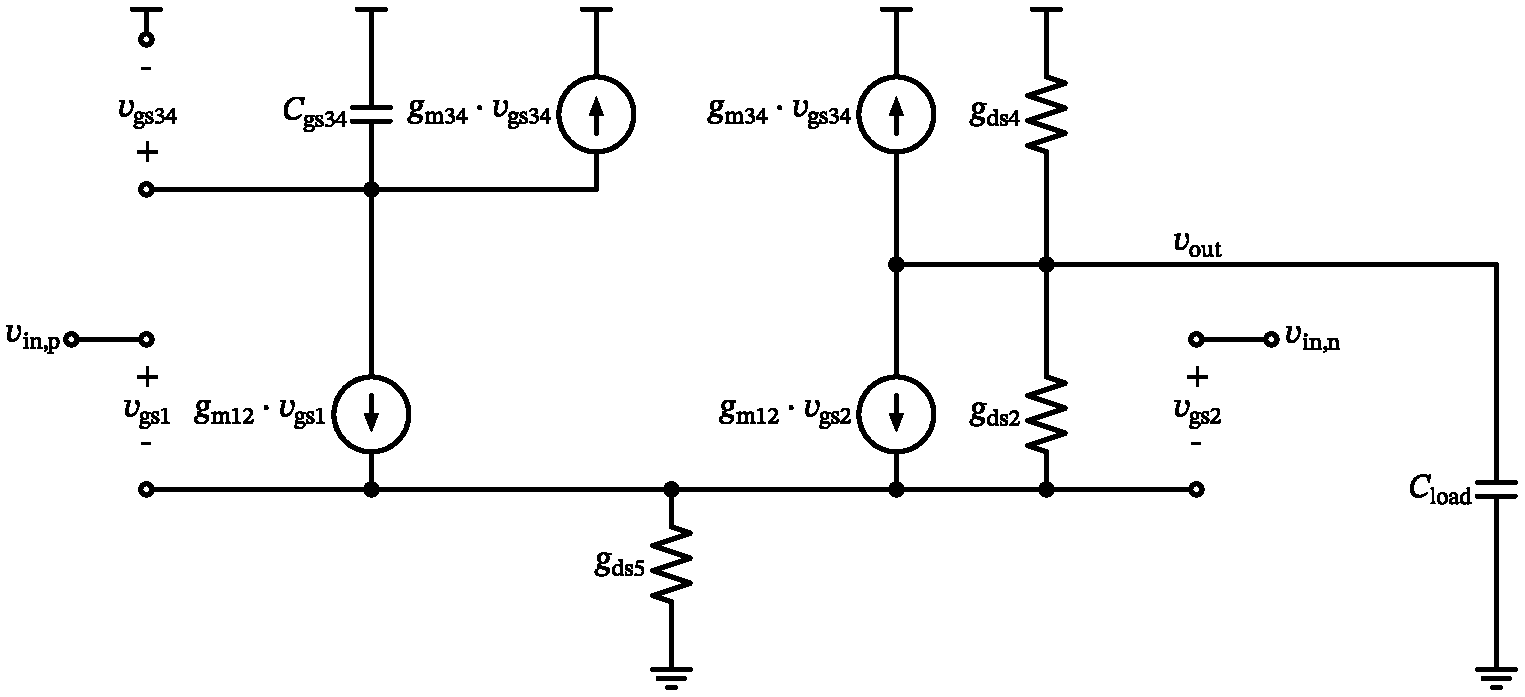
\includegraphics[keepaspectratio]{index_files/mediabag/index_files/figure-pdf/fig-basic-ota-small-signal-output-1.pdf}}

}

\caption{\label{fig-basic-ota-small-signal}5-transistor OTA small-signal
model.}

\end{figure}%

\textsubscript{Source:
\href{https://iic-jku.github.io/analog-circuit-design/index.qmd.html}{Article
Notebook}}

We can further simplify the output side by recognizing that the
impedance (when looking from the output down) is \(g_\mathrm{ds2}\) in
series with \(g_\mathrm{ds5} + g_\mathrm{m12}\). This is a valid
simplification as we treat \(M_1\) as a common-gate stage when looking
from the output, and since it is loaded by a low impedance of
\(g_\mathrm{m34}^{-1}\), we can approximate the impedance looking into
the source of \(M_1\) with \(g_\mathrm{m12}^{-1}\). With the
approximation that \(g_\mathrm{m}\gg g_\mathrm{ds}\) the parallel
connection of \(g_\mathrm{m12}\) and \(g_\mathrm{ds5}\) is dominated by
\(g_\mathrm{m12}\)
(\(g_\mathrm{m12} + g_\mathrm{ds5} \approx g_\mathrm{m12}\)) and its
series connection with \(g_\mathrm{ds2}\)
(\(g_\mathrm{m12}^{-1} + g_\mathrm{ds2}^{-1} \approx g_\mathrm{ds2}^{-1}\)),
resulting in the fact that we can ground the lower end of
\(g_\mathrm{ds2}\). You should probably stop here and read this
paragraph again, slowly.

Therefore, we can move \(g_\mathrm{ds2} + g_\mathrm{ds4}\) in parallel
to \(C_\mathrm{load}\). Further, assuming a differential drive with a
virtual ground at the tailpoint we can remove \(g_\mathrm{ds5}\). The
current source \(g_\mathrm{m34} v_\mathrm{gs34}\) is replaced with the
equivalent conductance \(g_\mathrm{m34}\). All the previous steps result
in the further simplified equivalent circuit shown in
Figure~\ref{fig-basic-ota-small-signal-simplified}.

\textsubscript{Source:
\href{https://iic-jku.github.io/analog-circuit-design/index.qmd.html}{Article
Notebook}}

\begin{figure}[H]

\centering{

\pandocbounded{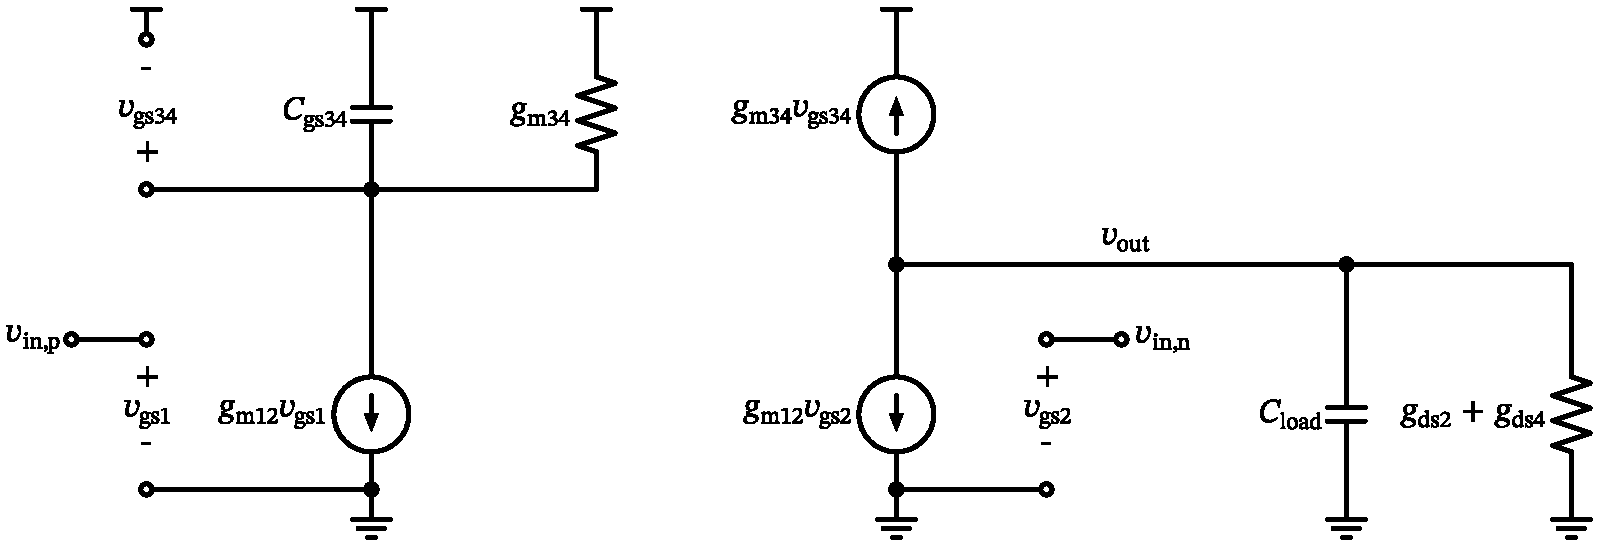
\includegraphics[keepaspectratio]{index_files/mediabag/index_files/figure-pdf/fig-basic-ota-small-signal-simplified-output-1.pdf}}

}

\caption{\label{fig-basic-ota-small-signal-simplified}5-transistor OTA
small-signal model with further simplifications.}

\end{figure}%

\textsubscript{Source:
\href{https://iic-jku.github.io/analog-circuit-design/index.qmd.html}{Article
Notebook}}

In the simplified circuit model in
Figure~\ref{fig-basic-ota-small-signal-simplified} we can see that we
have two poles in the circuit, one at the gate note of \(M_{3,4}\), and
one at the output. Realizing that \(v_\mathrm{in,p} = v_\mathrm{in}/2\)
and \(v_\mathrm{in,n} = - v_\mathrm{in}/2\) we can formulate KCL at the
output node to \begin{equation}\phantomsection\label{eq-simple-ota-eq1}{
-g_\mathrm{m34} V_\mathrm{gs34} - \left( -g_\mathrm{m12} \frac{V_\mathrm{in}}{2} \right) - V_\mathrm{out} (g_\mathrm{ds2} + g_\mathrm{ds4} + s C_\mathrm{load}) = 0.
}\end{equation} We further realize that
\begin{equation}\phantomsection\label{eq-simple-ota-eq2}{
V_\mathrm{gs34} = -g_\mathrm{m12} \frac{V_\mathrm{in}}{2} \frac{1}{g_\mathrm{m34} + s C_\mathrm{gs34}}.
 }\end{equation}

By combining Equation~\ref{eq-simple-ota-eq1} and
Equation~\ref{eq-simple-ota-eq2} and after a bit of algebraic
manipulation we arrive at
\begin{equation}\phantomsection\label{eq-simple-ota-gain}{
A(s) = \frac{V_\mathrm{out}(s)}{V_\mathrm{in}(s)} = \frac{g_\mathrm{m12}}{2} \frac{2 g_\mathrm{m34} + s C_\mathrm{gs34}}{(g_\mathrm{m34} + s C_\mathrm{gs34}) (g_\mathrm{ds2} + g_\mathrm{ds4} + s C_\mathrm{load})}.
}\end{equation}

When we now inspect Equation~\ref{eq-simple-ota-gain} we can see that
for low frequencies the (open-loop) gain is
\begin{equation}\phantomsection\label{eq-simple-ota-gain-dc}{
A(s \rightarrow 0) = A_0 = \frac{g_\mathrm{m12}}{g_\mathrm{ds2} + g_\mathrm{ds4}}
}\end{equation} which is plausible, and confirms the requirement of a
high impedance at the output node. For very large frequencies we get
\begin{equation}\phantomsection\label{eq-simple-ota-highf}{
A (s \gg) = \frac{g_\mathrm{m12}}{2 s C_\mathrm{load}}
}\end{equation} which is essentially the behavior of an integrator, and
we can use Equation~\ref{eq-simple-ota-highf} to calculate the frequency
where the gain drops to
\(|A(s_\mathrm{ug})| = 1 = g_\mathrm{m12}/|2 j \omega_\mathrm{ug} C_\mathrm{load}|\):
\[
f_\mathrm{ug} = \frac{g_\mathrm{m12}}{4 \pi C_\mathrm{load}}
\]

When looking at Equation~\ref{eq-simple-ota-gain} we see that we have a
dominant pole at \(s_\mathrm{p}\) and a pole-zero doublet with
\(s_\mathrm{pd}\)/\(s_\mathrm{zd}\):
\begin{equation}\phantomsection\label{eq-basic-ota-dominant-pole}{
s_\mathrm{p} = -\frac{g_\mathrm{ds2} + g_\mathrm{ds4}}{C_\mathrm{load}}
}\end{equation}
\begin{equation}\phantomsection\label{eq-basic-ota-doublet-pole}{
s_\mathrm{pd} = -\frac{g_\mathrm{m34}}{C_\mathrm{gs34}}
}\end{equation}
\begin{equation}\phantomsection\label{eq-basic-ota-doublet-zero}{
s_\mathrm{zd} = -\frac{2 g_\mathrm{m34}}{C_\mathrm{gs34}}
}\end{equation}

\begin{tcolorbox}[enhanced jigsaw, breakable, arc=.35mm, colbacktitle=quarto-callout-note-color!10!white, toprule=.15mm, left=2mm, toptitle=1mm, bottomtitle=1mm, opacityback=0, rightrule=.15mm, opacitybacktitle=0.6, titlerule=0mm, colback=white, colframe=quarto-callout-note-color-frame, coltitle=black, title=\textcolor{quarto-callout-note-color}{\faInfo}\hspace{0.5em}{Why a Pole-Zero Doublet?}, bottomrule=.15mm, leftrule=.75mm]

Looking at Equation~\ref{eq-basic-ota-doublet-pole} and
Equation~\ref{eq-basic-ota-doublet-zero} we see that this pair is
intimately linked by the same parameters and can only move together.
Hence we call it a ``doublet''. The effects of pole-zero doublets on the
frequency response and settling time of OTAs can be found in (Kamath,
Meyer, and Gray 1974). This paper shows that doublets may cause severe
degradation of settling time while only causing minor changes in the
frequency response of the amplifier.

\end{tcolorbox}

\subsubsection{OTA Noise}\label{ota-noise}

For the noise analysis we ignore the pole-zero doublet due to
\(C_\mathrm{gs34}\) (we assume minor impact due to this) and just
consider the dominant pole given by
Equation~\ref{eq-basic-ota-dominant-pole}. For the noise analysis at the
output we set the input signal to zero, and thus we arrive at the
simplified small-signal circuit shown in
Figure~\ref{fig-basic-ota-small-signal-noise}.

\textsubscript{Source:
\href{https://iic-jku.github.io/analog-circuit-design/index.qmd.html}{Article
Notebook}}

\begin{figure}[H]

\centering{

\pandocbounded{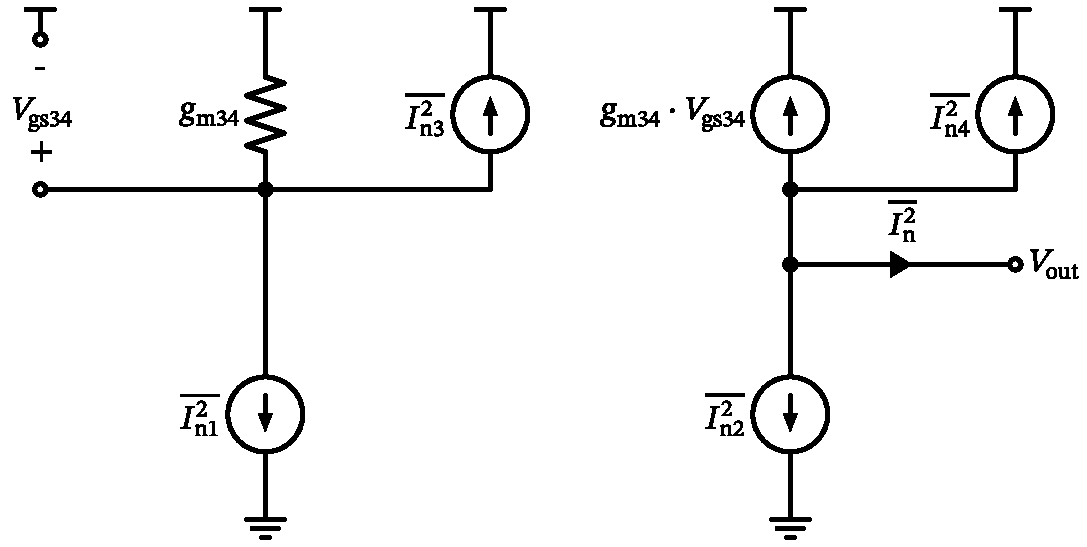
\includegraphics[keepaspectratio]{index_files/mediabag/index_files/figure-pdf/fig-basic-ota-small-signal-noise-output-1.pdf}}

}

\caption{\label{fig-basic-ota-small-signal-noise}5-transistor OTA
small-signal model for noise calculation.}

\end{figure}%

\textsubscript{Source:
\href{https://iic-jku.github.io/analog-circuit-design/index.qmd.html}{Article
Notebook}}

We see that \[
\overline{V_\mathrm{gs34}^2} = \frac{1}{g_\mathrm{m34}^2} \left( \overline{I_\mathrm{n1}^2} + \overline{I_\mathrm{n3}^2} \right).
\]

\begin{tcolorbox}[enhanced jigsaw, breakable, arc=.35mm, colbacktitle=quarto-callout-important-color!10!white, toprule=.15mm, left=2mm, toptitle=1mm, bottomtitle=1mm, opacityback=0, rightrule=.15mm, opacitybacktitle=0.6, titlerule=0mm, colback=white, colframe=quarto-callout-important-color-frame, coltitle=black, title=\textcolor{quarto-callout-important-color}{\faExclamation}\hspace{0.5em}{Noise Addition}, bottomrule=.15mm, leftrule=.75mm]

Remember that \textbf{uncorrelated} noise quantities need to be
power-summed (i.e., \(I^2 = I_1^2 + I_2^2\))!

\end{tcolorbox}

We can then sum the output noise current \(\overline{I_\mathrm{n}}\) as
\[
\overline{I_\mathrm{n}^2} = \overline{I_\mathrm{n2}^2} + \overline{I_\mathrm{n4}^2} + g_\mathrm{m34}^2 \frac{1}{g_\mathrm{m34}^2} \left( \overline{I_\mathrm{n1}^2} + \overline{I_\mathrm{n3}^2} \right) = 2 \left( \overline{I_\mathrm{n12}^2} + \overline{I_\mathrm{n34}^2} \right).
\]

As a next step, let us rewrite the OTA transfer function \(A(s)\) (see
Equation~\ref{eq-simple-ota-gain}) by getting rid of the pole-zero
doublet as a simplifying assumption to get
\begin{equation}\phantomsection\label{eq-simple-ota-gain-simplified}{
A'(s) = \frac{g_\mathrm{m12}}{g_\mathrm{ds2} + g_\mathrm{ds4} + s C_\mathrm{load}}.
}\end{equation}

Inspecting Equation~\ref{eq-simple-ota-gain-simplified} we can interpret
the OTA transfer function as a transconductor \(g_\mathrm{m12}\) driving
a load of
\(Y_\mathrm{load} = g_\mathrm{ds2} + g_\mathrm{ds4} + s C_\mathrm{load}\).
We can thus redraw Figure~\ref{fig-voltage-buffer-ota} in the following
way, injecting the previously calculated noise current into the output
node. The result is shown in Figure~\ref{fig-voltage-buffer-ota-noise}.

\textsubscript{Source:
\href{https://iic-jku.github.io/analog-circuit-design/index.qmd.html}{Article
Notebook}}

\begin{figure}[H]

\centering{

\pandocbounded{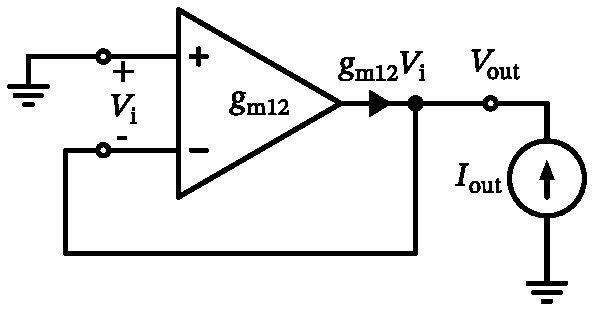
\includegraphics[keepaspectratio]{index_files/mediabag/index_files/figure-pdf/fig-voltage-buffer-ota-noise-zout-output-1.pdf}}

}

\caption{\label{fig-voltage-buffer-ota-noise-zout}Output impedance
calculation of a voltage buffer.}

\end{figure}%

\textsubscript{Source:
\href{https://iic-jku.github.io/analog-circuit-design/index.qmd.html}{Article
Notebook}}

\begin{tcolorbox}[enhanced jigsaw, breakable, arc=.35mm, colbacktitle=quarto-callout-note-color!10!white, toprule=.15mm, left=2mm, toptitle=1mm, bottomtitle=1mm, opacityback=0, rightrule=.15mm, opacitybacktitle=0.6, titlerule=0mm, colback=white, colframe=quarto-callout-note-color-frame, coltitle=black, title=\textcolor{quarto-callout-note-color}{\faInfo}\hspace{0.5em}{Output Impedance of the Voltage Buffer}, bottomrule=.15mm, leftrule=.75mm]

First we short the input terminal to ground and then we connect a
current source \(I_\mathrm{out}\) at the output terminal, see
Figure~\ref{fig-voltage-buffer-ota-noise-zout}. Since we can neglect the
gate leakage current into the inverting input terminal of the OTA, KCL
at the output node is simply: \[
I_\mathrm{out} + g_\mathrm{m12}\left(-V_\mathrm{out}\right) = 0
\] Thus, the output impedance is easily calculated. \[
Z_\mathrm{out} = \frac{V_\mathrm{out}}{I_\mathrm{out}} = \frac{V_\mathrm{out}}{g_\mathrm{m12}V_\mathrm{out}} = \frac{1}{g_\mathrm{m12}}
\]

\end{tcolorbox}

\textsubscript{Source:
\href{https://iic-jku.github.io/analog-circuit-design/index.qmd.html}{Article
Notebook}}

\begin{figure}[H]

\centering{

\pandocbounded{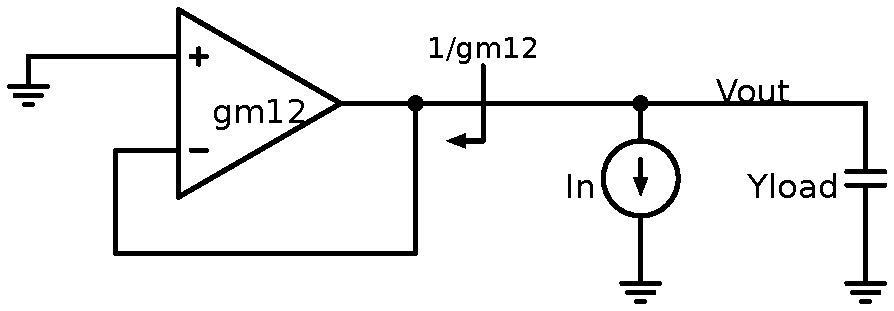
\includegraphics[keepaspectratio]{index_files/mediabag/index_files/figure-pdf/fig-voltage-buffer-ota-noise-output-1.pdf}}

}

\caption{\label{fig-voltage-buffer-ota-noise}The voltage buffer redrawn
for noise analysis.}

\end{figure}%

\textsubscript{Source:
\href{https://iic-jku.github.io/analog-circuit-design/index.qmd.html}{Article
Notebook}}

We see that the feedback around the transconductor \(g_\mathrm{m12}\)
creates an impedance of \(1/g_\mathrm{m12}\). We can now calculate the
effective load conductance of
\begin{equation}\phantomsection\label{eq-basic-ota-output-noise-yload}{
Y'_\mathrm{load} = g_\mathrm{ds2} + g_\mathrm{ds4} + s C_\mathrm{load} + g_\mathrm{m12} \approx g_\mathrm{m12} + s C_\mathrm{load}.
}\end{equation}

The output noise voltage is then (using Equation~\ref{eq-mosfet-noise})
\[
\overline{V_\mathrm{n,out}^2}(f) = \frac{\overline{I_\mathrm{n}^2}}{|Y'_\mathrm{load}|^2} = \frac{\overline{I_\mathrm{n}^2}}{g_\mathrm{m12}^2 + (2 \pi f C_\mathrm{load})2^2} = \frac{8 k T (\gamma_{12} g_\mathrm{m12} + \gamma_{34} g_\mathrm{m34})}{g_\mathrm{m12}^2 + (2 \pi f C_\mathrm{load})^2}.
\]

We can use the identity Equation~\ref{eq-integral-identity} to calculate
the rms output noise to
\begin{equation}\phantomsection\label{eq-basic-ota-output-noise}{
V_\mathrm{n,out,rms}^2 = \int_0^\infty \overline{V_\mathrm{n,out}^2}(f) df = \frac{k T}{C_\mathrm{load}} \left( 2 \gamma_{12} + 2 \gamma_{34} \frac{g_\mathrm{m34}}{g_\mathrm{m12}} \right).
}\end{equation}

Inspecting Equation~\ref{eq-basic-ota-output-noise} we can see that the
integrated output noise is the \(k T / C\) noise of the output load
capacitor, enhanced by the \(\gamma_{12}\) of the input differential
pair, plus a (smaller) contribution of the current mirror load
\(M_{3,4}\). Intuitively, this result makes sense.

\begin{tcolorbox}[enhanced jigsaw, breakable, arc=.35mm, colbacktitle=quarto-callout-tip-color!10!white, toprule=.15mm, left=2mm, toptitle=1mm, bottomtitle=1mm, opacityback=0, rightrule=.15mm, opacitybacktitle=0.6, titlerule=0mm, colback=white, colframe=quarto-callout-tip-color-frame, coltitle=black, title=\textcolor{quarto-callout-tip-color}{\faLightbulb}\hspace{0.5em}{Exercise: Derivation of 5T-OTA Performance}, bottomrule=.15mm, leftrule=.75mm]

Please take your time and carefully go through the explanations and
derivations for the 5-transistor-OTA in
Section~\ref{sec-basic-ota-large-signal} and
Section~\ref{sec-basic-ota-small-signal}. Try to do the calculations
yourself; if you get stuck, review the previous chapters.

\end{tcolorbox}

\subsection{5T-OTA Sizing}\label{sec-basic-ota-sizing}

Outfitted with the governing equations derived in
Section~\ref{sec-basic-ota-small-signal} we can now size the MOSFETs in
the OTA, we remember that we have to size \(M_{1,2}\) and \(M_{3,4}\)
equally.

First, we need to select a proper \(g_\mathrm{m}/I_\mathrm{D}\) for the
MOSFET. Remembering Section~\ref{sec-gmid-method} we see that for the
input differential pair we should go for a large \(g_\mathrm{m}\), thus
we select a \(g_\mathrm{m}/I_\mathrm{D}= 10\). As \(g_\mathrm{ds}\) of
\(M_2\) could limit the dc gain (Equation~\ref{eq-simple-ota-gain-dc})
we go with a rather long \(L = 5\,\mu\text{m}\). For current sources a
small \(g_\mathrm{m}/I_\mathrm{D}\) is a good idea, so we start with
\(g_\mathrm{m}/I_\mathrm{D}=5\) (because we can not go too low because
of \(V_\mathrm{ds,sat}\)) and also an \(L = 5\,\mu\text{m}\). The
\(g_\mathrm{m}/I_\mathrm{D}\) is also useful to estimate the required
drain-source voltage to keep a MOSFET in saturation (i.e., keep the
\(g_\mathrm{ds}\) small) with this approximate relationship:

\begin{equation}\phantomsection\label{eq-gmid-saturation}{
V_\mathrm{ds,sat} = \frac{2}{g_\mathrm{m}/I_\mathrm{D}}
}\end{equation}

\begin{tcolorbox}[enhanced jigsaw, breakable, arc=.35mm, colbacktitle=quarto-callout-tip-color!10!white, toprule=.15mm, left=2mm, toptitle=1mm, bottomtitle=1mm, opacityback=0, rightrule=.15mm, opacitybacktitle=0.6, titlerule=0mm, colback=white, colframe=quarto-callout-tip-color-frame, coltitle=black, title=\textcolor{quarto-callout-tip-color}{\faLightbulb}\hspace{0.5em}{Exercise: 5T-OTA Sizing}, bottomrule=.15mm, leftrule=.75mm]

Please size the 5T-OTA according to the previous
\(g_\mathrm{m}/I_\mathrm{D}\) and \(L\) suggestions. Please calculate
the \(W\) of \(M_{1-6}\) and the total supply current. Please check
wether gain error, total output noise, and turn-on settling is met with
the calculated devices sizes and bias currents.

\end{tcolorbox}

The sizing procedure and its calculation are best performed in a Jupyter
notebook, as we can easily look up the exact data from the pre-computed
tables:

\begin{tcolorbox}[enhanced jigsaw, breakable, arc=.35mm, colbacktitle=quarto-callout-tip-color!10!white, toprule=.15mm, left=2mm, toptitle=1mm, bottomtitle=1mm, opacityback=0, rightrule=.15mm, opacitybacktitle=0.6, titlerule=0mm, colback=white, colframe=quarto-callout-tip-color-frame, coltitle=black, title=\textcolor{quarto-callout-tip-color}{\faLightbulb}\hspace{0.5em}{Solution: 5T-OTA Sizing}, bottomrule=.15mm, leftrule=.75mm]

\section*{Sizing for Basic 5T-OTA}\label{sizing-for-basic-5t-ota}

\textbf{Copyright 2024 Harald Pretl}

Licensed under the Apache License, Version 2.0 (the ``License''); you
may not use this file except in compliance with the License. You may
obtain a copy of the License at
http://www.apache.org/licenses/LICENSE-2.0

\begin{Shaded}
\begin{Highlighting}[]
\CommentTok{\# read table data}
\ImportTok{from}\NormalTok{ pygmid }\ImportTok{import}\NormalTok{ Lookup }\ImportTok{as}\NormalTok{ lk}
\ImportTok{import}\NormalTok{ numpy }\ImportTok{as}\NormalTok{ np}
\NormalTok{lv\_nmos }\OperatorTok{=}\NormalTok{ lk(}\StringTok{\textquotesingle{}sg13\_lv\_nmos.mat\textquotesingle{}}\NormalTok{)}
\NormalTok{lv\_pmos }\OperatorTok{=}\NormalTok{ lk(}\StringTok{\textquotesingle{}sg13\_lv\_pmos.mat\textquotesingle{}}\NormalTok{)}
\CommentTok{\# list of parameters: VGS, VDS, VSB, L, W, NFING, ID, VT, GM, GMB, GDS, CGG, CGB, CGD, CGS, CDD, CSS, STH, SFL}
\CommentTok{\# if not specified, minimum L, VDS=max(vgs)/2=0.9 and VSB=0 are used }
\end{Highlighting}
\end{Shaded}

\begin{Shaded}
\begin{Highlighting}[]
\CommentTok{\# define the given parameters as taken from the specification table or inital guesses}
\NormalTok{c\_load }\OperatorTok{=} \FloatTok{50e{-}15}
\NormalTok{gm\_id\_m12 }\OperatorTok{=} \DecValTok{10}
\NormalTok{gm\_id\_m34 }\OperatorTok{=} \DecValTok{5}
\NormalTok{gm\_id\_m56 }\OperatorTok{=} \DecValTok{5}
\NormalTok{l\_12 }\OperatorTok{=} \DecValTok{5}
\NormalTok{l\_34 }\OperatorTok{=} \DecValTok{5}
\NormalTok{l\_56 }\OperatorTok{=} \DecValTok{5}
\NormalTok{f\_bw }\OperatorTok{=} \FloatTok{10e6}
\NormalTok{i\_total\_limit }\OperatorTok{=} \FloatTok{10e{-}6}
\NormalTok{i\_bias\_in }\OperatorTok{=} \FloatTok{20e{-}6}
\NormalTok{output\_voltage }\OperatorTok{=} \FloatTok{1.3}
\NormalTok{vin\_min }\OperatorTok{=} \FloatTok{0.7}
\NormalTok{vin\_max }\OperatorTok{=} \FloatTok{0.9}
\NormalTok{vdd\_min }\OperatorTok{=} \FloatTok{1.45}
\NormalTok{vdd\_max }\OperatorTok{=} \FloatTok{1.55}
\end{Highlighting}
\end{Shaded}

\begin{Shaded}
\begin{Highlighting}[]
\CommentTok{\# we get the required gm of M1/2 from the bandwidth requirement}
\CommentTok{\# we add a factor of 3 to allow for PVT variation plus additional MOSFET parasitic loading}
\NormalTok{gm\_m12 }\OperatorTok{=}\NormalTok{ f\_bw }\OperatorTok{*} \DecValTok{3} \OperatorTok{*} \DecValTok{4}\OperatorTok{*}\NormalTok{np.pi}\OperatorTok{*}\NormalTok{c\_load}
\BuiltInTok{print}\NormalTok{(}\StringTok{\textquotesingle{}gm12 =\textquotesingle{}}\NormalTok{, }\BuiltInTok{round}\NormalTok{(gm\_m12}\OperatorTok{/}\FloatTok{1e{-}3}\NormalTok{, }\DecValTok{4}\NormalTok{), }\StringTok{\textquotesingle{}mS\textquotesingle{}}\NormalTok{)}
\end{Highlighting}
\end{Shaded}

\begin{verbatim}
gm12 = 0.0188 mS
\end{verbatim}

\begin{Shaded}
\begin{Highlighting}[]
\CommentTok{\# since we know gm12 and the gmid we can calculate the bias current}
\NormalTok{id\_m12 }\OperatorTok{=}\NormalTok{ gm\_m12 }\OperatorTok{/}\NormalTok{ gm\_id\_m12}
\NormalTok{i\_total }\OperatorTok{=} \DecValTok{2}\OperatorTok{*}\NormalTok{id\_m12}
\BuiltInTok{print}\NormalTok{(}\StringTok{\textquotesingle{}i\_total (exact) =\textquotesingle{}}\NormalTok{, }\BuiltInTok{round}\NormalTok{(i\_total}\OperatorTok{/}\FloatTok{1e{-}6}\NormalTok{, }\DecValTok{1}\NormalTok{), }\StringTok{\textquotesingle{}µA\textquotesingle{}}\NormalTok{)}
\CommentTok{\# we round to 0.5µA bias currents}
\NormalTok{i\_total }\OperatorTok{=} \BuiltInTok{max}\NormalTok{(}\BuiltInTok{round}\NormalTok{(i\_total }\OperatorTok{/} \FloatTok{1e{-}6} \OperatorTok{*} \DecValTok{2}\NormalTok{) }\OperatorTok{/} \DecValTok{2} \OperatorTok{*} \FloatTok{1e{-}6}\NormalTok{, }\FloatTok{0.5e{-}6}\NormalTok{)}
\NormalTok{id\_m12 }\OperatorTok{=}\NormalTok{ i\_total}\OperatorTok{/}\DecValTok{2}

\BuiltInTok{print}\NormalTok{(}\StringTok{\textquotesingle{}i\_total (rounded) =\textquotesingle{}}\NormalTok{, i\_total}\OperatorTok{/}\FloatTok{1e{-}6}\NormalTok{, }\StringTok{\textquotesingle{}µA\textquotesingle{}}\NormalTok{)}
\ControlFlowTok{if}\NormalTok{ i\_total }\OperatorTok{\textless{}}\NormalTok{ i\_total\_limit:}
    \BuiltInTok{print}\NormalTok{(}\StringTok{\textquotesingle{}[info] power consumption target is met!\textquotesingle{}}\NormalTok{)}
\ControlFlowTok{else}\NormalTok{:}
    \BuiltInTok{print}\NormalTok{(}\StringTok{\textquotesingle{}[info] power consumption target is NOT met!\textquotesingle{}}\NormalTok{) }
\end{Highlighting}
\end{Shaded}

\begin{verbatim}
i_total (exact) = 3.8 µA
i_total (rounded) = 4.0 µA
[info] power consumption target is met!
\end{verbatim}

\begin{Shaded}
\begin{Highlighting}[]
\CommentTok{\# we calculate the dc gain}
\NormalTok{gm\_gds\_m12 }\OperatorTok{=}\NormalTok{ lv\_nmos.lookup(}\StringTok{\textquotesingle{}GM\_GDS\textquotesingle{}}\NormalTok{, GM\_ID}\OperatorTok{=}\NormalTok{gm\_id\_m12, L}\OperatorTok{=}\NormalTok{l\_12, VDS}\OperatorTok{=}\FloatTok{0.75}\NormalTok{, VSB}\OperatorTok{=}\DecValTok{0}\NormalTok{)}
\NormalTok{gm\_gds\_m34 }\OperatorTok{=}\NormalTok{ lv\_pmos.lookup(}\StringTok{\textquotesingle{}GM\_GDS\textquotesingle{}}\NormalTok{, GM\_ID}\OperatorTok{=}\NormalTok{gm\_id\_m34, L}\OperatorTok{=}\NormalTok{l\_34, VDS}\OperatorTok{=}\FloatTok{0.75}\NormalTok{, VSB}\OperatorTok{=}\DecValTok{0}\NormalTok{)}

\NormalTok{gds\_m12 }\OperatorTok{=}\NormalTok{ gm\_m12 }\OperatorTok{/}\NormalTok{ gm\_gds\_m12}
\NormalTok{gm\_m34 }\OperatorTok{=}\NormalTok{ gm\_id\_m34 }\OperatorTok{*}\NormalTok{ i\_total}\OperatorTok{/}\DecValTok{2}
\NormalTok{gds\_m34 }\OperatorTok{=}\NormalTok{ gm\_m34 }\OperatorTok{/}\NormalTok{ gm\_gds\_m34}

\NormalTok{a0 }\OperatorTok{=}\NormalTok{ gm\_m12 }\OperatorTok{/}\NormalTok{ (gds\_m12 }\OperatorTok{+}\NormalTok{ gds\_m34)}
\BuiltInTok{print}\NormalTok{(}\StringTok{\textquotesingle{}a0 =\textquotesingle{}}\NormalTok{, }\BuiltInTok{round}\NormalTok{(}\DecValTok{20}\OperatorTok{*}\NormalTok{np.log10(a0), }\DecValTok{1}\NormalTok{), }\StringTok{\textquotesingle{}dB\textquotesingle{}}\NormalTok{)}
\end{Highlighting}
\end{Shaded}

\begin{verbatim}
a0 = 34.8 dB
\end{verbatim}

\begin{Shaded}
\begin{Highlighting}[]
\CommentTok{\# we calculate the MOSFET capacitance which adds to Cload, to see the impact on the BW}
\NormalTok{gm\_cgs\_m12 }\OperatorTok{=}\NormalTok{ lv\_nmos.lookup(}\StringTok{\textquotesingle{}GM\_CGS\textquotesingle{}}\NormalTok{, GM\_ID}\OperatorTok{=}\NormalTok{gm\_id\_m12, L}\OperatorTok{=}\NormalTok{l\_12, VDS}\OperatorTok{=}\FloatTok{0.75}\NormalTok{, VSB}\OperatorTok{=}\DecValTok{0}\NormalTok{)}
\NormalTok{gm\_cdd\_m12 }\OperatorTok{=}\NormalTok{ lv\_nmos.lookup(}\StringTok{\textquotesingle{}GM\_CDD\textquotesingle{}}\NormalTok{, GM\_ID}\OperatorTok{=}\NormalTok{gm\_id\_m12, L}\OperatorTok{=}\NormalTok{l\_12, VDS}\OperatorTok{=}\FloatTok{0.75}\NormalTok{, VSB}\OperatorTok{=}\DecValTok{0}\NormalTok{)}
\NormalTok{gm\_cdd\_m34 }\OperatorTok{=}\NormalTok{ lv\_pmos.lookup(}\StringTok{\textquotesingle{}GM\_CDD\textquotesingle{}}\NormalTok{, GM\_ID}\OperatorTok{=}\NormalTok{gm\_id\_m34, L}\OperatorTok{=}\NormalTok{l\_34, VDS}\OperatorTok{=}\FloatTok{0.75}\NormalTok{, VSB}\OperatorTok{=}\DecValTok{0}\NormalTok{)}

\NormalTok{c\_load\_parasitic }\OperatorTok{=} \BuiltInTok{abs}\NormalTok{(gm\_m12}\OperatorTok{/}\NormalTok{gm\_cgs\_m12) }\OperatorTok{+} \BuiltInTok{abs}\NormalTok{(gm\_m12}\OperatorTok{/}\NormalTok{gm\_cdd\_m12) }\OperatorTok{+} \BuiltInTok{abs}\NormalTok{(gm\_m34}\OperatorTok{/}\NormalTok{gm\_cdd\_m34)}
\BuiltInTok{print}\NormalTok{(}\StringTok{\textquotesingle{}additional load capacitance =\textquotesingle{}}\NormalTok{, }\BuiltInTok{round}\NormalTok{(c\_load\_parasitic}\OperatorTok{/}\FloatTok{1e{-}15}\NormalTok{, }\DecValTok{1}\NormalTok{), }\StringTok{\textquotesingle{}fF\textquotesingle{}}\NormalTok{)}

\NormalTok{f\_bw }\OperatorTok{=}\NormalTok{ gm\_m12 }\OperatorTok{/}\NormalTok{ (}\DecValTok{4}\OperatorTok{*}\NormalTok{np.pi }\OperatorTok{*}\NormalTok{ (c\_load }\OperatorTok{+}\NormalTok{ c\_load\_parasitic))}
\BuiltInTok{print}\NormalTok{(}\StringTok{\textquotesingle{}{-}3dB bandwidth incl. parasitics =\textquotesingle{}}\NormalTok{, }\BuiltInTok{round}\NormalTok{(f\_bw}\OperatorTok{/}\FloatTok{1e6}\NormalTok{, }\DecValTok{2}\NormalTok{), }\StringTok{\textquotesingle{}MHz\textquotesingle{}}\NormalTok{)}
\end{Highlighting}
\end{Shaded}

\begin{verbatim}
additional load capacitance = 54.9 fF
-3dB bandwidth incl. parasitics = 14.3 MHz
\end{verbatim}

\begin{Shaded}
\begin{Highlighting}[]
\CommentTok{\# we can now look up the VGS of the MOSFET}
\NormalTok{vgs\_m12 }\OperatorTok{=}\NormalTok{ lv\_nmos.look\_upVGS(GM\_ID}\OperatorTok{=}\NormalTok{gm\_id\_m12, L}\OperatorTok{=}\NormalTok{l\_12, VDS}\OperatorTok{=}\FloatTok{0.75}\NormalTok{, VSB}\OperatorTok{=}\FloatTok{0.0}\NormalTok{)}
\NormalTok{vgs\_m34 }\OperatorTok{=}\NormalTok{ lv\_pmos.look\_upVGS(GM\_ID}\OperatorTok{=}\NormalTok{gm\_id\_m34, L}\OperatorTok{=}\NormalTok{l\_34, VDS}\OperatorTok{=}\FloatTok{0.75}\NormalTok{, VSB}\OperatorTok{=}\FloatTok{0.0}\NormalTok{) }
\NormalTok{vgs\_m56 }\OperatorTok{=}\NormalTok{ lv\_nmos.look\_upVGS(GM\_ID}\OperatorTok{=}\NormalTok{gm\_id\_m56, L}\OperatorTok{=}\NormalTok{l\_56, VDS}\OperatorTok{=}\FloatTok{0.75}\NormalTok{, VSB}\OperatorTok{=}\FloatTok{0.0}\NormalTok{) }

\BuiltInTok{print}\NormalTok{(}\StringTok{\textquotesingle{}vgs\_12 =\textquotesingle{}}\NormalTok{, }\BuiltInTok{round}\NormalTok{(}\BuiltInTok{float}\NormalTok{(vgs\_m12), }\DecValTok{3}\NormalTok{), }\StringTok{\textquotesingle{}V\textquotesingle{}}\NormalTok{)}
\BuiltInTok{print}\NormalTok{(}\StringTok{\textquotesingle{}vgs\_34 =\textquotesingle{}}\NormalTok{, }\BuiltInTok{round}\NormalTok{(}\BuiltInTok{float}\NormalTok{(vgs\_m34), }\DecValTok{3}\NormalTok{), }\StringTok{\textquotesingle{}V\textquotesingle{}}\NormalTok{)}
\BuiltInTok{print}\NormalTok{(}\StringTok{\textquotesingle{}vgs\_56 =\textquotesingle{}}\NormalTok{, }\BuiltInTok{round}\NormalTok{(}\BuiltInTok{float}\NormalTok{(vgs\_m56), }\DecValTok{3}\NormalTok{), }\StringTok{\textquotesingle{}V\textquotesingle{}}\NormalTok{)}
\end{Highlighting}
\end{Shaded}

\begin{verbatim}
vgs_12 = 0.367 V
vgs_34 = 0.729 V
vgs_56 = 0.591 V
\end{verbatim}

\begin{Shaded}
\begin{Highlighting}[]
\CommentTok{\# calculate settling time due to slewing with the calculated bias current}
\NormalTok{t\_slew }\OperatorTok{=}\NormalTok{ (c\_load }\OperatorTok{+}\NormalTok{ c\_load\_parasitic) }\OperatorTok{*}\NormalTok{ output\_voltage }\OperatorTok{/}\NormalTok{ i\_total}
\BuiltInTok{print}\NormalTok{(}\StringTok{\textquotesingle{}slewing time =\textquotesingle{}}\NormalTok{, }\BuiltInTok{round}\NormalTok{(t\_slew}\OperatorTok{/}\FloatTok{1e{-}6}\NormalTok{, }\DecValTok{3}\NormalTok{), }\StringTok{\textquotesingle{}µs\textquotesingle{}}\NormalTok{)}
\NormalTok{t\_settle }\OperatorTok{=} \DecValTok{5}\OperatorTok{/}\NormalTok{(}\DecValTok{2}\OperatorTok{*}\NormalTok{np.pi}\OperatorTok{*}\NormalTok{f\_bw)}
\BuiltInTok{print}\NormalTok{(}\StringTok{\textquotesingle{}settling time =\textquotesingle{}}\NormalTok{, }\BuiltInTok{round}\NormalTok{(t\_settle}\OperatorTok{/}\FloatTok{1e{-}6}\NormalTok{, }\DecValTok{3}\NormalTok{), }\StringTok{\textquotesingle{}µs\textquotesingle{}}\NormalTok{)}
\end{Highlighting}
\end{Shaded}

\begin{verbatim}
slewing time = 0.034 µs
settling time = 0.056 µs
\end{verbatim}

\begin{Shaded}
\begin{Highlighting}[]
\CommentTok{\# calculate voltage gain error}
\NormalTok{gain\_error }\OperatorTok{=}\NormalTok{ a0 }\OperatorTok{/}\NormalTok{ (}\DecValTok{1} \OperatorTok{+}\NormalTok{ a0)}
\BuiltInTok{print}\NormalTok{(}\StringTok{\textquotesingle{}voltage gain error =\textquotesingle{}}\NormalTok{, }\BuiltInTok{round}\NormalTok{((gain\_error}\OperatorTok{{-}}\DecValTok{1}\NormalTok{)}\OperatorTok{*}\DecValTok{100}\NormalTok{, }\DecValTok{1}\NormalTok{), }\StringTok{\textquotesingle{}\%\textquotesingle{}}\NormalTok{)}
\end{Highlighting}
\end{Shaded}

\begin{verbatim}
voltage gain error = -1.8 %
\end{verbatim}

\begin{Shaded}
\begin{Highlighting}[]
\CommentTok{\# calculate total rms output noise}
\NormalTok{sth\_m12 }\OperatorTok{=}\NormalTok{ lv\_nmos.lookup(}\StringTok{\textquotesingle{}STH\_GM\textquotesingle{}}\NormalTok{, VGS}\OperatorTok{=}\NormalTok{vgs\_m12, L}\OperatorTok{=}\NormalTok{l\_12, VDS}\OperatorTok{=}\FloatTok{0.75}\NormalTok{, VSB}\OperatorTok{=}\DecValTok{0}\NormalTok{) }\OperatorTok{*}\NormalTok{ gm\_m12}
\NormalTok{gamma\_m12 }\OperatorTok{=}\NormalTok{ sth\_m12}\OperatorTok{/}\NormalTok{(}\DecValTok{4}\OperatorTok{*}\FloatTok{1.38e{-}23}\OperatorTok{*}\DecValTok{300}\OperatorTok{*}\NormalTok{gm\_m12)}

\NormalTok{sth\_m34 }\OperatorTok{=}\NormalTok{ lv\_pmos.lookup(}\StringTok{\textquotesingle{}STH\_GM\textquotesingle{}}\NormalTok{, VGS}\OperatorTok{=}\NormalTok{vgs\_m34, L}\OperatorTok{=}\NormalTok{l\_34, VDS}\OperatorTok{=}\FloatTok{0.75}\NormalTok{, VSB}\OperatorTok{=}\DecValTok{0}\NormalTok{) }\OperatorTok{*}\NormalTok{ gm\_m34}
\NormalTok{gamma\_m34 }\OperatorTok{=}\NormalTok{ sth\_m34}\OperatorTok{/}\NormalTok{(}\DecValTok{4}\OperatorTok{*}\FloatTok{1.38e{-}23}\OperatorTok{*}\DecValTok{300}\OperatorTok{*}\NormalTok{gm\_m34)}

\NormalTok{output\_noise\_rms }\OperatorTok{=} \FloatTok{1.38e{-}23}\OperatorTok{*}\DecValTok{300} \OperatorTok{/}\NormalTok{ (c\_load }\OperatorTok{+}\NormalTok{ c\_load\_parasitic) }\OperatorTok{*}\NormalTok{ (}\DecValTok{2}\OperatorTok{*}\NormalTok{gamma\_m12 }\OperatorTok{+} \DecValTok{2}\OperatorTok{*}\NormalTok{gamma\_m34 }\OperatorTok{*}\NormalTok{ gm\_m34}\OperatorTok{/}\NormalTok{gm\_m12)}
\BuiltInTok{print}\NormalTok{(}\StringTok{\textquotesingle{}output noise (rms) =\textquotesingle{}}\NormalTok{, }\BuiltInTok{round}\NormalTok{(output\_noise\_rms}\OperatorTok{/}\FloatTok{1e{-}6}\NormalTok{, }\DecValTok{4}\NormalTok{), }\StringTok{\textquotesingle{}µV\textquotesingle{}}\NormalTok{)}
\end{Highlighting}
\end{Shaded}

\begin{verbatim}
output noise (rms) = 0.1254 µV
\end{verbatim}

\begin{Shaded}
\begin{Highlighting}[]
\CommentTok{\# calculate all widths}
\NormalTok{id\_w\_m12 }\OperatorTok{=}\NormalTok{ lv\_nmos.lookup(}\StringTok{\textquotesingle{}ID\_W\textquotesingle{}}\NormalTok{, GM\_ID}\OperatorTok{=}\NormalTok{gm\_id\_m12, L}\OperatorTok{=}\NormalTok{l\_12, VDS}\OperatorTok{=}\NormalTok{vgs\_m12, VSB}\OperatorTok{=}\DecValTok{0}\NormalTok{)}
\NormalTok{w\_12 }\OperatorTok{=}\NormalTok{ id\_m12 }\OperatorTok{/}\NormalTok{ id\_w\_m12}
\NormalTok{w\_12\_round }\OperatorTok{=} \BuiltInTok{max}\NormalTok{(}\BuiltInTok{round}\NormalTok{(w\_12}\OperatorTok{*}\DecValTok{2}\NormalTok{)}\OperatorTok{/}\DecValTok{2}\NormalTok{, }\FloatTok{0.5}\NormalTok{)}
\BuiltInTok{print}\NormalTok{(}\StringTok{\textquotesingle{}M1/2 W =\textquotesingle{}}\NormalTok{, }\BuiltInTok{round}\NormalTok{(w\_12, }\DecValTok{2}\NormalTok{), }\StringTok{\textquotesingle{}um, rounded W =\textquotesingle{}}\NormalTok{, w\_12\_round, }\StringTok{\textquotesingle{}um\textquotesingle{}}\NormalTok{)}

\NormalTok{id\_m34 }\OperatorTok{=}\NormalTok{ id\_m12}
\NormalTok{id\_w\_m34 }\OperatorTok{=}\NormalTok{ lv\_pmos.lookup(}\StringTok{\textquotesingle{}ID\_W\textquotesingle{}}\NormalTok{, GM\_ID}\OperatorTok{=}\NormalTok{gm\_id\_m34, L}\OperatorTok{=}\NormalTok{l\_34, VDS}\OperatorTok{=}\NormalTok{vgs\_m34, VSB}\OperatorTok{=}\DecValTok{0}\NormalTok{)}
\NormalTok{w\_34 }\OperatorTok{=}\NormalTok{ id\_m34 }\OperatorTok{/}\NormalTok{ id\_w\_m34}
\NormalTok{w\_34\_round }\OperatorTok{=} \BuiltInTok{max}\NormalTok{(}\BuiltInTok{round}\NormalTok{(w\_34}\OperatorTok{*}\DecValTok{2}\NormalTok{)}\OperatorTok{/}\DecValTok{2}\NormalTok{, }\FloatTok{0.5}\NormalTok{) }
\BuiltInTok{print}\NormalTok{(}\StringTok{\textquotesingle{}M3/4 W =\textquotesingle{}}\NormalTok{, }\BuiltInTok{round}\NormalTok{(w\_34, }\DecValTok{2}\NormalTok{), }\StringTok{\textquotesingle{}um, rounded W =\textquotesingle{}}\NormalTok{, w\_34\_round, }\StringTok{\textquotesingle{}um\textquotesingle{}}\NormalTok{)}

\NormalTok{id\_w\_m5 }\OperatorTok{=}\NormalTok{ lv\_nmos.lookup(}\StringTok{\textquotesingle{}ID\_W\textquotesingle{}}\NormalTok{, GM\_ID}\OperatorTok{=}\NormalTok{gm\_id\_m56, L}\OperatorTok{=}\NormalTok{l\_56, VDS}\OperatorTok{=}\NormalTok{vgs\_m56, VSB}\OperatorTok{=}\DecValTok{0}\NormalTok{)}
\NormalTok{w\_5 }\OperatorTok{=}\NormalTok{ i\_total }\OperatorTok{/}\NormalTok{ id\_w\_m5}
\NormalTok{w\_5\_round }\OperatorTok{=} \BuiltInTok{max}\NormalTok{(}\BuiltInTok{round}\NormalTok{(w\_5}\OperatorTok{*}\DecValTok{2}\NormalTok{)}\OperatorTok{/}\DecValTok{2}\NormalTok{, }\FloatTok{0.5}\NormalTok{)}
\BuiltInTok{print}\NormalTok{(}\StringTok{\textquotesingle{}M5 W =\textquotesingle{}}\NormalTok{, }\BuiltInTok{round}\NormalTok{(w\_5, }\DecValTok{2}\NormalTok{), }\StringTok{\textquotesingle{}um, rounded W =\textquotesingle{}}\NormalTok{, w\_5\_round, }\StringTok{\textquotesingle{}um\textquotesingle{}}\NormalTok{)}
\NormalTok{w\_6 }\OperatorTok{=}\NormalTok{ w\_5\_round }\OperatorTok{*}\NormalTok{ i\_bias\_in }\OperatorTok{/}\NormalTok{ i\_total}
\NormalTok{w\_6\_round }\OperatorTok{=} \BuiltInTok{max}\NormalTok{(}\BuiltInTok{round}\NormalTok{(w\_6}\OperatorTok{*}\DecValTok{2}\NormalTok{)}\OperatorTok{/}\DecValTok{2}\NormalTok{, }\FloatTok{0.5}\NormalTok{)}
\BuiltInTok{print}\NormalTok{(}\StringTok{\textquotesingle{}M6 W =\textquotesingle{}}\NormalTok{, }\BuiltInTok{round}\NormalTok{(w\_6\_round, }\DecValTok{2}\NormalTok{), }\StringTok{\textquotesingle{}um\textquotesingle{}}\NormalTok{)}
\end{Highlighting}
\end{Shaded}

\begin{verbatim}
M1/2 W = 1.77 um, rounded W = 2.0 um
M3/4 W = 1.64 um, rounded W = 1.5 um
M5 W = 0.74 um, rounded W = 0.5 um
M6 W = 2.5 um
\end{verbatim}

\begin{Shaded}
\begin{Highlighting}[]
\CommentTok{\# print out final design values}
\BuiltInTok{print}\NormalTok{(}\StringTok{\textquotesingle{}5T{-}OTA dimensioning:\textquotesingle{}}\NormalTok{)}
\BuiltInTok{print}\NormalTok{(}\StringTok{\textquotesingle{}{-}{-}{-}{-}{-}{-}{-}{-}{-}{-}{-}{-}{-}{-}{-}{-}{-}{-}{-}{-}\textquotesingle{}}\NormalTok{)}
\BuiltInTok{print}\NormalTok{(}\StringTok{\textquotesingle{}M1/2 W=\textquotesingle{}}\NormalTok{, w\_12\_round, }\StringTok{\textquotesingle{}, L=\textquotesingle{}}\NormalTok{, l\_12)}
\BuiltInTok{print}\NormalTok{(}\StringTok{\textquotesingle{}M3/4 W=\textquotesingle{}}\NormalTok{, w\_34\_round, }\StringTok{\textquotesingle{}, L=\textquotesingle{}}\NormalTok{, l\_34)}
\BuiltInTok{print}\NormalTok{(}\StringTok{\textquotesingle{}M5   W=\textquotesingle{}}\NormalTok{, w\_5\_round, }\StringTok{\textquotesingle{}, L=\textquotesingle{}}\NormalTok{, l\_56)}
\BuiltInTok{print}\NormalTok{(}\StringTok{\textquotesingle{}M6   W=\textquotesingle{}}\NormalTok{, w\_6\_round, }\StringTok{\textquotesingle{}, L=\textquotesingle{}}\NormalTok{, l\_56)}
\BuiltInTok{print}\NormalTok{()}
\BuiltInTok{print}\NormalTok{(}\StringTok{\textquotesingle{}5T{-}OTA performance summary:\textquotesingle{}}\NormalTok{)}
\BuiltInTok{print}\NormalTok{(}\StringTok{\textquotesingle{}{-}{-}{-}{-}{-}{-}{-}{-}{-}{-}{-}{-}{-}{-}{-}{-}{-}{-}{-}{-}{-}{-}{-}{-}{-}{-}{-}\textquotesingle{}}\NormalTok{)}
\BuiltInTok{print}\NormalTok{(}\StringTok{\textquotesingle{}supply current =\textquotesingle{}}\NormalTok{, }\BuiltInTok{round}\NormalTok{(i\_total}\OperatorTok{/}\FloatTok{1e{-}6}\NormalTok{, }\DecValTok{1}\NormalTok{), }\StringTok{\textquotesingle{}µA\textquotesingle{}}\NormalTok{)}
\BuiltInTok{print}\NormalTok{(}\StringTok{\textquotesingle{}output noise =\textquotesingle{}}\NormalTok{, }\BuiltInTok{round}\NormalTok{(output\_noise\_rms}\OperatorTok{/}\FloatTok{1e{-}6}\NormalTok{, }\DecValTok{4}\NormalTok{), }\StringTok{\textquotesingle{}µVrms\textquotesingle{}}\NormalTok{)}
\BuiltInTok{print}\NormalTok{(}\StringTok{\textquotesingle{}voltage gain error =\textquotesingle{}}\NormalTok{, }\BuiltInTok{round}\NormalTok{((gain\_error}\OperatorTok{{-}}\DecValTok{1}\NormalTok{)}\OperatorTok{*}\DecValTok{100}\NormalTok{, }\DecValTok{1}\NormalTok{), }\StringTok{\textquotesingle{}\%\textquotesingle{}}\NormalTok{)}
\BuiltInTok{print}\NormalTok{(}\StringTok{\textquotesingle{}{-}3dB bandwidth incl. parasitics =\textquotesingle{}}\NormalTok{, }\BuiltInTok{round}\NormalTok{(f\_bw}\OperatorTok{/}\FloatTok{1e6}\NormalTok{, }\DecValTok{2}\NormalTok{), }\StringTok{\textquotesingle{}MHz\textquotesingle{}}\NormalTok{)}
\BuiltInTok{print}\NormalTok{(}\StringTok{\textquotesingle{}turn{-}on time (slewing+settling) =\textquotesingle{}}\NormalTok{, }\BuiltInTok{round}\NormalTok{((t\_slew}\OperatorTok{+}\NormalTok{t\_settle)}\OperatorTok{/}\FloatTok{1e{-}6}\NormalTok{, }\DecValTok{3}\NormalTok{), }\StringTok{\textquotesingle{}µs\textquotesingle{}}\NormalTok{)}
\BuiltInTok{print}\NormalTok{()}
\BuiltInTok{print}\NormalTok{(}\StringTok{\textquotesingle{}5T{-}OTA bias point check:\textquotesingle{}}\NormalTok{)}
\BuiltInTok{print}\NormalTok{(}\StringTok{\textquotesingle{}{-}{-}{-}{-}{-}{-}{-}{-}{-}{-}{-}{-}{-}{-}{-}{-}{-}{-}{-}{-}{-}{-}{-}{-}\textquotesingle{}}\NormalTok{)}
\BuiltInTok{print}\NormalTok{(}\StringTok{\textquotesingle{}headroom M1 =\textquotesingle{}}\NormalTok{, }\BuiltInTok{round}\NormalTok{(vdd\_min}\OperatorTok{{-}}\NormalTok{vgs\_m34}\OperatorTok{+}\NormalTok{vgs\_m12}\OperatorTok{{-}}\NormalTok{vin\_max, }\DecValTok{3}\NormalTok{), }\StringTok{\textquotesingle{}V\textquotesingle{}}\NormalTok{)}
\BuiltInTok{print}\NormalTok{(}\StringTok{\textquotesingle{}headroom M4 =\textquotesingle{}}\NormalTok{, }\BuiltInTok{round}\NormalTok{(vdd\_min}\OperatorTok{{-}}\NormalTok{vin\_max, }\DecValTok{3}\NormalTok{), }\StringTok{\textquotesingle{}V\textquotesingle{}}\NormalTok{)}
\BuiltInTok{print}\NormalTok{(}\StringTok{\textquotesingle{}headroom M5 =\textquotesingle{}}\NormalTok{, }\BuiltInTok{round}\NormalTok{(vin\_min}\OperatorTok{{-}}\NormalTok{vgs\_m12, }\DecValTok{3}\NormalTok{), }\StringTok{\textquotesingle{}V\textquotesingle{}}\NormalTok{)}
\end{Highlighting}
\end{Shaded}

\begin{verbatim}
5T-OTA dimensioning:
--------------------
M1/2 W= 2.0 , L= 5
M3/4 W= 1.5 , L= 5
M5   W= 0.5 , L= 5
M6   W= 2.5 , L= 5

5T-OTA performance summary:
---------------------------
supply current = 4.0 µA
output noise = 0.1254 µVrms
voltage gain error = -1.8 %
-3dB bandwidth incl. parasitics = 14.3 MHz
turn-on time (slewing+settling) = 0.09 µs

5T-OTA bias point check:
------------------------
headroom M1 = 0.188 V
headroom M4 = 0.55 V
headroom M5 = 0.333 V
\end{verbatim}

\textsubscript{Source:
\href{https://iic-jku.github.io/analog-circuit-design/sizing/sizing_basic_ota-preview.html\#cell-0}{Sizing
for Basic 5T-OTA}}

\end{tcolorbox}

\subsection{5T-OTA Simulation}\label{sec-basic-ota-simulation}

With the initial sizing of the MOSFETs of the 5T-OTA done, we can design
the 5T-OTA circuit and setup a simulation testbench to check the
performance parameters. Since this is the first time we draw a more
complex schematic, and use a hierarchical design, we should note that
drawing a schematic is an art, and there exists a set of rules and
recommendations how to name pins, how to use annotations, and so on.
Please read Section~\ref{sec-designers-etiquette} before you start into
your design work.

\begin{tcolorbox}[enhanced jigsaw, breakable, arc=.35mm, colbacktitle=quarto-callout-tip-color!10!white, toprule=.15mm, left=2mm, toptitle=1mm, bottomtitle=1mm, opacityback=0, rightrule=.15mm, opacitybacktitle=0.6, titlerule=0mm, colback=white, colframe=quarto-callout-tip-color-frame, coltitle=black, title=\textcolor{quarto-callout-tip-color}{\faLightbulb}\hspace{0.5em}{Exercise: 5T-OTA Design and Testbench}, bottomrule=.15mm, leftrule=.75mm]

Please design the circuit of the 5T-OTA. Put the OTA circuit in a
separate schematic, create a symbol for it, and use this symbol in a
testbench you create in Xschem for this 5T-OTA used as a voltage buffer
as shown in Figure~\ref{fig-voltage-buffer-ota}. Use typical conditions
for the simulation, and check how well the specification in
Table~\ref{tbl-voltage-buffer-spec} is met, and how well the derivations
in Section~\ref{sec-basic-ota-large-signal} and
Section~\ref{sec-basic-ota-small-signal} fit to the simulation results.

If you get stuck, you can find the testbench and 5T-OTA schematic
\href{./xschem/ota-5t_tb-ac.svg}{here} (for the small-signal analysis)
and \href{./xschem/ota-5t_tb-tran.svg}{here} (for the large-signal
settling simulation). For interested students, the loop gain analysis
with Middlebrook's and Tian's method of the 5T-OTA can be found
\href{./xschem/ota-5t_tb-loopgain.svg}{here}.

\end{tcolorbox}

\subsection{5T-OTA Simulation versus
PVT}\label{t-ota-simulation-versus-pvt}

As you have seen in Section~\ref{sec-basic-ota-simulation} running
simulations by hand is tedious. When we want to check the overall
performance, we have to run many simulations over various conditions:

\begin{enumerate}
\def\labelenumi{\arabic{enumi}.}
\tightlist
\item
  The supply voltage of the circuit has tolerances, and thus we need to
  check the performance against this variation.
\item
  The temperature at which the circuit is operated is likely changing.
  Also the performance against this has to be verified.
\item
  When manufacturing the wafers random variations in various process
  parameters lead to changed parameters of the integrated circuit
  components. In order to check for this effect, wafer foundries provide
  model files which shall cover these manufacturing excursions.
  Simplified, this leads to a slower or faster MOSFET, and usually NMOS
  and PMOS are not correlated, so we have the process corners
  \textbf{SS}, \textbf{SF}, \textbf{TT}, \textbf{FS}, and \textbf{FF}.
  So far, we have only used the \textbf{TT} models in our simulations.
\end{enumerate}

The variations listed in the previous list are abbreviated as
\textbf{PVT} (process, voltage, temperature) variations. In order to
finalize a circuit all combinations of these (plus the variations in
operating conditions like input voltage) have to be simulated. As you
can imagine, this leads to a huge number of simulations, and simulation
results which have to be evaluated for pass/fail.

There are two options how to tackle this efficiently:

\begin{enumerate}
\def\labelenumi{\arabic{enumi}.}
\tightlist
\item
  As an experienced designer you have a very solid understanding of the
  circuit, plus based on the analytic equations you can identify which
  combination of operating conditions will lead to a worst case
  performance. Thus, you can drastically reduce the number of corners to
  simulate, and you run them by hand.
\item
  You are using a framework which highly automates this task of running
  a plethora of different simulations and evaluating the outcome. These
  frameworks are called simulation runners.
\end{enumerate}

Luckily, there are open-source versions of simulation runners available,
and we will use \href{https://github.com/efabless/cace}{CACE} in this
lecture. CACE is written in Python and allows to setup a datasheet in
\href{https://yaml.org}{YAML} which defines the simulation problem and
the performance parameters to evaluate against which limits. The
resulting simulations are then run in parallel and the simulation data
is evaluated and summarized in various forms.

There is a CACE setup available for our 5T-OTA. The
\href{./cace/voltage-buffer-ota.yaml}{datasheet} describes the operating
conditions and the simulations tasks. For each simulation a testbench
template is needed, \href{./cace/templates/ota-5t-ac.sch}{this one} is
used for ac simulations, \href{./cace/templates/ota-5t-noise.sch}{this
one} is used for noise simulation, and
\href{./cace/templates/ota-5t-tran.sch}{this one} is used for transient
simulation.

After a successful run, a documentation is automatically generated. The
result of a full run of this \href{./xschem/ota-5t.svg}{OTA design} is
presented here:

\begin{tcolorbox}[enhanced jigsaw, breakable, arc=.35mm, colbacktitle=quarto-callout-note-color!10!white, toprule=.15mm, left=2mm, toptitle=1mm, bottomtitle=1mm, opacityback=0, rightrule=.15mm, opacitybacktitle=0.6, titlerule=0mm, colback=white, colframe=quarto-callout-note-color-frame, coltitle=black, title=\textcolor{quarto-callout-note-color}{\faInfo}\hspace{0.5em}{Note \ref*{nte-basic-ota-cace-result}: CACE Summary for 5T-OTA}, bottomrule=.15mm, leftrule=.75mm]

\quartocalloutnte{nte-basic-ota-cace-result} 

\section*{CACE Summary for ota-5t}\label{cace-summary-for-ota-5t}

\textbf{netlist source}: schematic

\begin{longtable}[]{@{}
  >{\raggedright\arraybackslash}p{(\linewidth - 18\tabcolsep) * \real{0.1550}}
  >{\raggedright\arraybackslash}p{(\linewidth - 18\tabcolsep) * \real{0.1550}}
  >{\raggedright\arraybackslash}p{(\linewidth - 18\tabcolsep) * \real{0.1163}}
  >{\raggedleft\arraybackslash}p{(\linewidth - 18\tabcolsep) * \real{0.0775}}
  >{\raggedleft\arraybackslash}p{(\linewidth - 18\tabcolsep) * \real{0.0930}}
  >{\raggedleft\arraybackslash}p{(\linewidth - 18\tabcolsep) * \real{0.0775}}
  >{\raggedleft\arraybackslash}p{(\linewidth - 18\tabcolsep) * \real{0.0930}}
  >{\raggedleft\arraybackslash}p{(\linewidth - 18\tabcolsep) * \real{0.0775}}
  >{\raggedleft\arraybackslash}p{(\linewidth - 18\tabcolsep) * \real{0.0930}}
  >{\centering\arraybackslash}p{(\linewidth - 18\tabcolsep) * \real{0.0620}}@{}}
\toprule\noalign{}
\begin{minipage}[b]{\linewidth}\raggedright
Parameter
\end{minipage} & \begin{minipage}[b]{\linewidth}\raggedright
Tool
\end{minipage} & \begin{minipage}[b]{\linewidth}\raggedright
Result
\end{minipage} & \begin{minipage}[b]{\linewidth}\raggedleft
Min Limit
\end{minipage} & \begin{minipage}[b]{\linewidth}\raggedleft
Min Value
\end{minipage} & \begin{minipage}[b]{\linewidth}\raggedleft
Typ Target
\end{minipage} & \begin{minipage}[b]{\linewidth}\raggedleft
Typ Value
\end{minipage} & \begin{minipage}[b]{\linewidth}\raggedleft
Max Limit
\end{minipage} & \begin{minipage}[b]{\linewidth}\raggedleft
Max Value
\end{minipage} & \begin{minipage}[b]{\linewidth}\centering
Status
\end{minipage} \\
\midrule\noalign{}
\endhead
\bottomrule\noalign{}
\endlastfoot
Output voltage ratio & ngspice & gain & 0.97 V/V & 0.987 V/V & any &
1.000 V/V & 1.03 V/V & 1.006 V/V & Pass ✅ \\
Bandwidth & ngspice & bw & 10e6 Hz & 15551000.000 Hz & any &
26912100.000 Hz & any & 34051700.000 Hz & Pass ✅ \\
Output noise & ngspice & noise & any & 0.308 mV & any & 0.371 mV & 1 mV
& 0.455 mV & Pass ✅ \\
Settling time & ngspice & tsettle & any & 0.135 us & any & 0.142 us & 10
us & 0.155 us & Pass ✅ \\
\end{longtable}

\subsection*{Plots}\label{plots}

\subsection*{gain\_vs\_temp}\label{gain_vs_temp}

\begin{figure}[H]

{\centering \pandocbounded{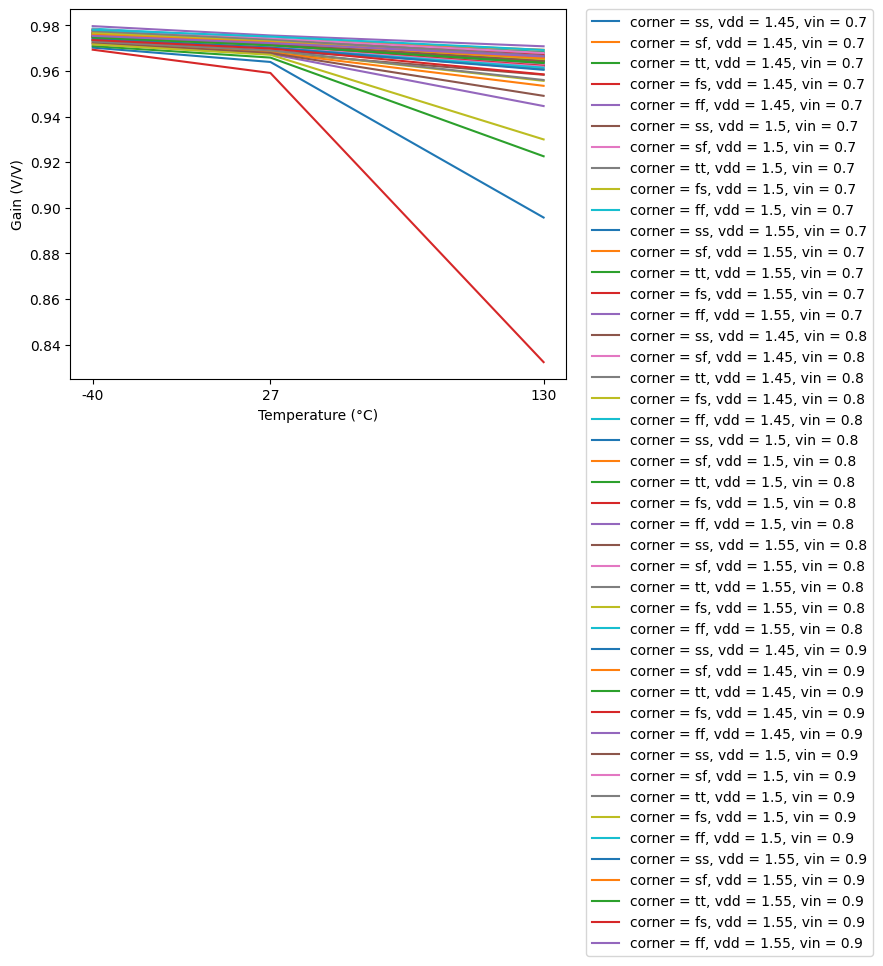
\includegraphics[keepaspectratio]{./cace/_docs/ota-5t/schematic/gain_vs_temp.png}}

}

\caption{gain\_vs\_temp}

\end{figure}%

\subsection*{gain\_vs\_vin}\label{gain_vs_vin}

\begin{figure}[H]

{\centering \pandocbounded{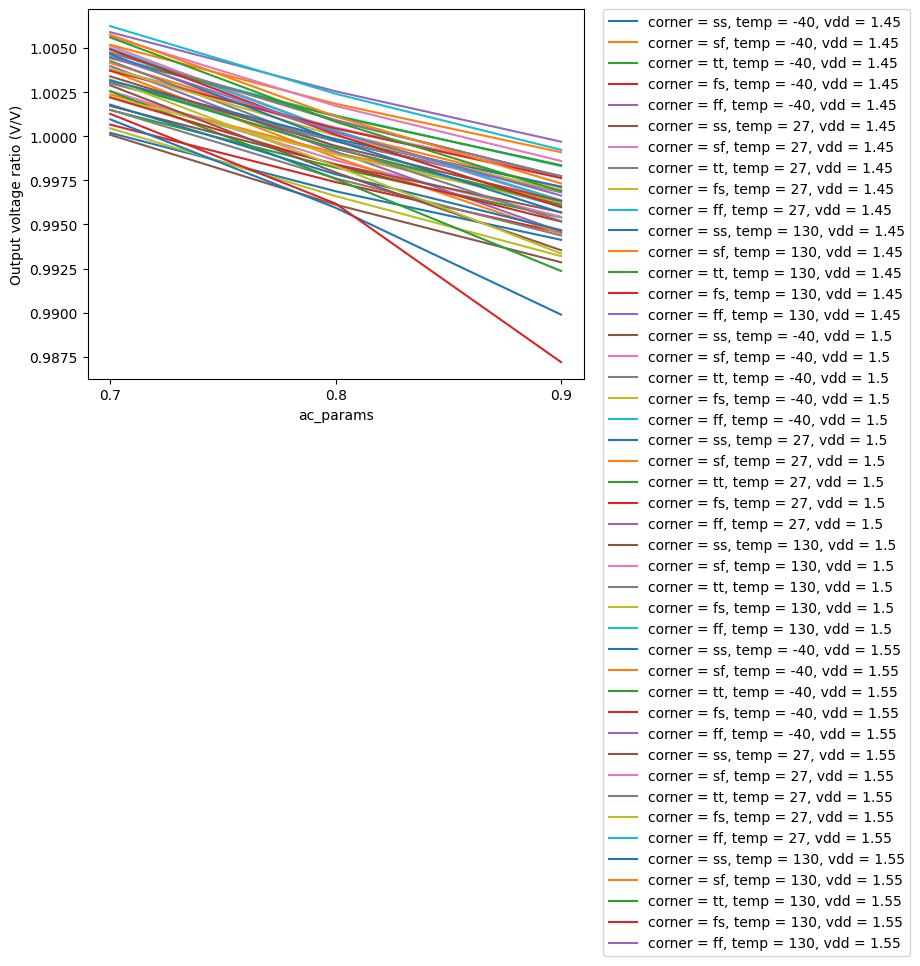
\includegraphics[keepaspectratio]{./cace/_docs/ota-5t/schematic/gain_vs_vin.png}}

}

\caption{gain\_vs\_vin}

\end{figure}%

\subsection*{gain\_vs\_vdd}\label{gain_vs_vdd}

\begin{figure}[H]

{\centering \pandocbounded{\includegraphics[keepaspectratio]{./cace/_docs/ota-5t/schematic/gain_vs_vdd.png}}

}

\caption{gain\_vs\_vdd}

\end{figure}%

\subsection*{gain\_vs\_corner}\label{gain_vs_corner}

\begin{figure}[H]

{\centering \pandocbounded{\includegraphics[keepaspectratio]{./cace/_docs/ota-5t/schematic/gain_vs_corner.png}}

}

\caption{gain\_vs\_corner}

\end{figure}%

\subsection*{bw\_vs\_temp}\label{bw_vs_temp}

\begin{figure}[H]

{\centering \pandocbounded{\includegraphics[keepaspectratio]{./cace/_docs/ota-5t/schematic/bw_vs_temp.png}}

}

\caption{bw\_vs\_temp}

\end{figure}%

\subsection*{bw\_vs\_vin}\label{bw_vs_vin}

\begin{figure}[H]

{\centering \pandocbounded{\includegraphics[keepaspectratio]{./cace/_docs/ota-5t/schematic/bw_vs_vin.png}}

}

\caption{bw\_vs\_vin}

\end{figure}%

\subsection*{bw\_vs\_vdd}\label{bw_vs_vdd}

\begin{figure}[H]

{\centering \pandocbounded{\includegraphics[keepaspectratio]{./cace/_docs/ota-5t/schematic/bw_vs_vdd.png}}

}

\caption{bw\_vs\_vdd}

\end{figure}%

\subsection*{bw\_vs\_corner}\label{bw_vs_corner}

\begin{figure}[H]

{\centering \pandocbounded{\includegraphics[keepaspectratio]{./cace/_docs/ota-5t/schematic/bw_vs_corner.png}}

}

\caption{bw\_vs\_corner}

\end{figure}%

\subsection*{noise\_vs\_temp}\label{noise_vs_temp}

\begin{figure}[H]

{\centering \pandocbounded{\includegraphics[keepaspectratio]{./cace/_docs/ota-5t/schematic/noise_vs_temp.png}}

}

\caption{noise\_vs\_temp}

\end{figure}%

\subsection*{noise\_vs\_vin}\label{noise_vs_vin}

\begin{figure}[H]

{\centering \pandocbounded{\includegraphics[keepaspectratio]{./cace/_docs/ota-5t/schematic/noise_vs_vin.png}}

}

\caption{noise\_vs\_vin}

\end{figure}%

\subsection*{noise\_vs\_vdd}\label{noise_vs_vdd}

\begin{figure}[H]

{\centering \pandocbounded{\includegraphics[keepaspectratio]{./cace/_docs/ota-5t/schematic/noise_vs_vdd.png}}

}

\caption{noise\_vs\_vdd}

\end{figure}%

\subsection*{noise\_vs\_corner}\label{noise_vs_corner}

\begin{figure}[H]

{\centering \pandocbounded{\includegraphics[keepaspectratio]{./cace/_docs/ota-5t/schematic/noise_vs_corner.png}}

}

\caption{noise\_vs\_corner}

\end{figure}%

\subsection*{settling\_vs\_temp}\label{settling_vs_temp}

\begin{figure}[H]

{\centering \pandocbounded{\includegraphics[keepaspectratio]{./cace/_docs/ota-5t/schematic/settling_vs_temp.png}}

}

\caption{settling\_vs\_temp}

\end{figure}%

\subsection*{settling\_vs\_vin}\label{settling_vs_vin}

\begin{figure}[H]

{\centering \pandocbounded{\includegraphics[keepaspectratio]{./cace/_docs/ota-5t/schematic/settling_vs_vin.png}}

}

\caption{settling\_vs\_vin}

\end{figure}%

\subsection*{settling\_vs\_vdd}\label{settling_vs_vdd}

\begin{figure}[H]

{\centering \pandocbounded{\includegraphics[keepaspectratio]{./cace/_docs/ota-5t/schematic/settling_vs_vdd.png}}

}

\caption{settling\_vs\_vdd}

\end{figure}%

\subsection*{settling\_vs\_corner}\label{settling_vs_corner}

\begin{figure}[H]

{\centering \pandocbounded{\includegraphics[keepaspectratio]{./cace/_docs/ota-5t/schematic/settling_vs_corner.png}}

}

\caption{settling\_vs\_corner}

\end{figure}%

\end{tcolorbox}

\subsubsection{PVT Simulation Analysis}\label{pvt-simulation-analysis}

Looking at the CACE report in Note~\ref{nte-basic-ota-cace-result} we
see that (luckily) the specification is met for all parameters. This is
great news! We now have a design that we carefully simulated across PVT
and other corners, and which is ready for layout. Once we have the
layout ready, we can extract the wiring parasitic (\(R\) and \(C\)) as
well as other layout-dependent effects like
\href{https://global.oup.com/us/companion.websites/9780195170153/pdf/proximityeffectmodels.pdf}{well
proximity}. Using this augmented netlist we can then again use CACE to
check performance across conditions and parameter variations, and if we
still pass all specification points then our design is finished.

\subsection{OTA Variants}\label{sec-ota-variants-single-ended}

Following, we are going to discuss two popular variants of the simple
5T-OTA. The first version provides an almost rail-to-rail single-ended
output, and can thus be used for a variety of applications requiring
this range. The arrangement is shown in
Figure~\ref{fig-ota-se-rail-to-rail}. It is a single-stage amplifier, as
the only high-impedance point is at the output where significant
voltage-gain is produced. The current mirrors can be used to scale up
the current generated in the input differential pair to some extent in
the output stage (or can be used to lower the current compared to the
bias current in the diffpair); i.e., the bias currents of the input
stage and the output stage can be set independently.

Being a single-stage amplifier stability is usually not an issue, as
only the output node is high-ohmic; all other nodes feature a MOSFET
diode so the node impedance is \(\approx g_\mathrm{m}^{-1}\) and thus
the according poles are located at high frequencies.

\textsubscript{Source:
\href{https://iic-jku.github.io/analog-circuit-design/index.qmd.html}{Article
Notebook}}

\begin{figure}[H]

\centering{

\pandocbounded{\includegraphics[keepaspectratio]{index_files/mediabag/index_files/figure-pdf/fig-ota-se-rail-to-rail-output-1.pdf}}

}

\caption{\label{fig-ota-se-rail-to-rail}Single-ended OTA with
rail-to-rail output stage.}

\end{figure}%

\textsubscript{Source:
\href{https://iic-jku.github.io/analog-circuit-design/index.qmd.html}{Article
Notebook}}

Another popular version is shown in Figure~\ref{fig-ota-se-twostage}.
Here, we have a two-stage amplifier able to provide higher voltage gain.
The first stage (the diffpair loaded by a current mirror) is followed by
a single-stage common-source amplifier with current-source load. Being a
two-stage amplifier with two high-ohmic nodes, stability is a concern,
so usually we need some form of compensation.
Figure~\ref{fig-ota-se-twostage} shows a very simplistic
Miller-compensation using \(C_\mathrm{M}\). Often, we would want to
implement a more advanced scheme. Some examples can be found in (Baker,
n.d.). An interesting technique is the indirect compensation with
cascoded input differential pairs (see Figure~\ref{fig-improved-ota})
for higher power supply rejection. An advantage of this two-stage
amplifier (compared with the simple 5T-OTA) is the dc-balanced load on
top of the differential pair, as each side sees a voltage drop from
\(V_\mathrm{DD}\) of one \(V_\mathrm{GS}\) (\(V_\mathrm{GS3}\) on the
left side, \(V_\mathrm{GS5}\) on the right side).

\textsubscript{Source:
\href{https://iic-jku.github.io/analog-circuit-design/index.qmd.html}{Article
Notebook}}

\begin{figure}[H]

\centering{

\pandocbounded{\includegraphics[keepaspectratio]{index_files/mediabag/index_files/figure-pdf/fig-ota-se-twostage-output-1.pdf}}

}

\caption{\label{fig-ota-se-twostage}Single-ended two-stage OTA with
rail-to-rail output.}

\end{figure}%

\textsubscript{Source:
\href{https://iic-jku.github.io/analog-circuit-design/index.qmd.html}{Article
Notebook}}

Note that the circuit of Figure~\ref{fig-ota-se-twostage} can be easily
modified into a low-dropout voltage regulator (LDO). This simple yet
often effective circuit is shown in Figure~\ref{fig-simple-ldo}. The
pass transistor \(M_\mathrm{pass}\) has to be sized according to the
load current and the dropout voltage.

\textsubscript{Source:
\href{https://iic-jku.github.io/analog-circuit-design/index.qmd.html}{Article
Notebook}}

\begin{figure}[H]

\centering{

\pandocbounded{\includegraphics[keepaspectratio]{index_files/mediabag/index_files/figure-pdf/fig-simple-ldo-output-1.pdf}}

}

\caption{\label{fig-simple-ldo}A basic low-dropout voltage regulator
(LDO) with Miller compensation.}

\end{figure}%

\textsubscript{Source:
\href{https://iic-jku.github.io/analog-circuit-design/index.qmd.html}{Article
Notebook}}

The reference voltage \(V_\mathrm{ref}\) is scaled by \(R_1\) and
\(R_2\), so that the output voltage \(V_\mathrm{out}\) is given by

\[
V_\mathrm{out} \approx V_\mathrm{ref} \left( 1 + \frac{R_1}{R_2} \right)
\]

if the gain of the OTA is sufficiently high. The quiescent current
through \(R_{1,2}\) establishes a minimum load current for the LDO,
which is often good for stability. More information on LDOs can be found
in (Razavi 2019).

\section{Cascode Stage}\label{sec-cascode-stage}

As we have seen in Section~\ref{sec-basic-ota} the performance of the
OTA is generally quite acceptable (see
Table~\ref{tbl-voltage-buffer-spec}), but we might want to aim for
better output voltage accuracy. As our analysis has shown the output
voltage tolerance is limited by the open-loop dc gain \(A_0\) of the OTA
(see Equation~\ref{eq-voltage-buffer-tolerance}), which in turn is
limited by the output conductance of \(M_2\) and \(M_4\) in
Figure~\ref{fig-basic-ota}, which is also confirmed by the analytical
result in Equation~\ref{eq-simple-ota-gain-dc}.

During the sizing procedure we have seen that the achievable
\(g_\mathrm{m}/ g_\mathrm{ds}\) ratio of a single MOSFET is limited,
even if we increase \(L\). We are thus searching for a better option,
and here (local) feedback in form of a \textbf{cascode} comes to help.

For analysis of a cascode, we use the following single-transistor stage
shown in Figure~\ref{fig-cascode-transistor}.

\textsubscript{Source:
\href{https://iic-jku.github.io/analog-circuit-design/index.qmd.html}{Article
Notebook}}

\begin{figure}[H]

\centering{

\pandocbounded{\includegraphics[keepaspectratio]{index_files/mediabag/index_files/figure-pdf/fig-cascode-transistor-output-1.pdf}}

}

\caption{\label{fig-cascode-transistor}A MOSFET cascode circuit.}

\end{figure}%

\textsubscript{Source:
\href{https://iic-jku.github.io/analog-circuit-design/index.qmd.html}{Article
Notebook}}

In order to derive the operation of the cascode analytically, we draw
the small-signal equivalent circuit in
Figure~\ref{fig-cascode-small-signal}. We assume that \(V_\mathrm{B}\)
is a low-ohmic bias voltage, thus we replace it by ac ground. We further
set \(g_\mathrm{mb}= 0\).

\textsubscript{Source:
\href{https://iic-jku.github.io/analog-circuit-design/index.qmd.html}{Article
Notebook}}

\begin{figure}[H]

\centering{

\pandocbounded{\includegraphics[keepaspectratio]{index_files/mediabag/index_files/figure-pdf/fig-cascode-small-signal-output-1.pdf}}

}

\caption{\label{fig-cascode-small-signal}The MOSFET cascode small-signal
model.}

\end{figure}%

\textsubscript{Source:
\href{https://iic-jku.github.io/analog-circuit-design/index.qmd.html}{Article
Notebook}}

Since the gate is assumed at a fixed potential, we can put
\(C_\mathrm{gs}\) in parallel to \(G_\mathrm{S}\) as
\(G_\mathrm{S}^{*} = G_\mathrm{S} + s C_\mathrm{gs}\), and we can put
\(C_\mathrm{gd}\) in parallel to \(G_\mathrm{D}\) as
\(G_\mathrm{D}^{*} = G_\mathrm{D} + s C_\mathrm{gd}\). As a result we
will disregard these capacitors for now, and just consider
\(G_\mathrm{S}\) and \(G_\mathrm{D}\).

\textsubscript{Source:
\href{https://iic-jku.github.io/analog-circuit-design/index.qmd.html}{Article
Notebook}}

\begin{figure}[H]

\centering{

\pandocbounded{\includegraphics[keepaspectratio]{index_files/mediabag/index_files/figure-pdf/fig-cascode-small-signal-simplified-output-1.pdf}}

}

\caption{\label{fig-cascode-small-signal-simplified}The simplified
MOSFET cascode small-signal model.}

\end{figure}%

\textsubscript{Source:
\href{https://iic-jku.github.io/analog-circuit-design/index.qmd.html}{Article
Notebook}}

\subsection{Cascode Output Impedance}\label{cascode-output-impedance}

As a first step, we want to calculate the output impedance at the drain
of the MOSFET (i.e., looking into the drain). For this, we replace
\(G_\mathrm{D}\) with a current source. The resulting small-signal
equivalent circuit is shown in
Figure~\ref{fig-cascode-small-signal-simplified-out}.

\textsubscript{Source:
\href{https://iic-jku.github.io/analog-circuit-design/index.qmd.html}{Article
Notebook}}

\begin{figure}[H]

\centering{

\pandocbounded{\includegraphics[keepaspectratio]{index_files/mediabag/index_files/figure-pdf/fig-cascode-small-signal-simplified-out-output-1.pdf}}

}

\caption{\label{fig-cascode-small-signal-simplified-out}The simplified
MOSFET cascode small-signal model for calculation of the output
impedance.}

\end{figure}%

\textsubscript{Source:
\href{https://iic-jku.github.io/analog-circuit-design/index.qmd.html}{Article
Notebook}}

We realize that \(i_\mathrm{out}\) flows through \(G_\mathrm{S}\) and
drops \(v_\mathrm{gs}\) (note the sign): \[
v_\mathrm{gs}= -\frac{i_\mathrm{out}}{G_\mathrm{S}}
\]

Further, \(v_\mathrm{out} = -v_\mathrm{gs}+ v_\mathrm{ds}\). Calculating
KCL at the output node results in \[
i_\mathrm{out} - g_\mathrm{m}v_\mathrm{gs}- g_\mathrm{ds}v_\mathrm{ds}= 0.
\]

Using the previously found identities, and after a bit of algebraic
manipulations we arrive at
\begin{equation}\phantomsection\label{eq-cascode-output}{
g_\mathrm{out} = \frac{i_\mathrm{out}}{v_\mathrm{out}} = \frac{g_\mathrm{ds}}{1 + \frac{g_\mathrm{m}+ g_\mathrm{ds}}{G_\mathrm{S}}} = \frac{g_\mathrm{ds}\cdot G_\mathrm{S}}{G_\mathrm{S} + g_\mathrm{m}+ g_\mathrm{ds}}
}\end{equation}

We find that if \(G_\mathrm{S} = 0\) (an open) then
\(g_\mathrm{out} = 0\), and if \(G_\mathrm{S} = \infty\) (a short) then
\(g_\mathrm{out} = g_\mathrm{ds}\). We can calculate the benefits of a
cascode if we assume we put a cascode on top of a common-source
transistor stage (thus \(G_\mathrm{S} = g_\mathrm{ds}'\)) and get
\begin{equation}\phantomsection\label{eq-cs-cascode-output-impedance}{
g_\mathrm{out} = \frac{g_\mathrm{ds}\cdot g_\mathrm{ds}'}{g_\mathrm{ds}' + g_\mathrm{m}+ g_\mathrm{ds}} \approx g_\mathrm{ds}' \frac{g_\mathrm{ds}}{g_\mathrm{m}}.
}\end{equation}

\begin{tcolorbox}[enhanced jigsaw, breakable, arc=.35mm, colbacktitle=quarto-callout-important-color!10!white, toprule=.15mm, left=2mm, toptitle=1mm, bottomtitle=1mm, opacityback=0, rightrule=.15mm, opacitybacktitle=0.6, titlerule=0mm, colback=white, colframe=quarto-callout-important-color-frame, coltitle=black, title=\textcolor{quarto-callout-important-color}{\faExclamation}\hspace{0.5em}{Benefit of Cascode (Output)}, bottomrule=.15mm, leftrule=.75mm]

The output impedance of the lower MOSFET (\(g_\mathrm{ds}'\)) is
\textbf{reduced} by the self-gain of the cascode transistor! This is a
powerful technique to increase the output impedance of a transistor
stage by cascoding, much better than increasing \(L\).

\end{tcolorbox}

\subsection{Cascode Input Impedance}\label{cascode-input-impedance}

To calculate the input impedance of a cascode (i.e., looking into the
source) we replace \(G_\mathrm{S}\) with a current source. The resulting
small-signal equivalent circuit is shown in
Figure~\ref{fig-cascode-small-signal-simplified-in}.

\textsubscript{Source:
\href{https://iic-jku.github.io/analog-circuit-design/index.qmd.html}{Article
Notebook}}

\begin{figure}[H]

\centering{

\pandocbounded{\includegraphics[keepaspectratio]{index_files/mediabag/index_files/figure-pdf/fig-cascode-small-signal-simplified-in-output-1.pdf}}

}

\caption{\label{fig-cascode-small-signal-simplified-in}The simplified
MOSFET cascode small-signal model for calculation of the input
impedance.}

\end{figure}%

\textsubscript{Source:
\href{https://iic-jku.github.io/analog-circuit-design/index.qmd.html}{Article
Notebook}}

We note that \(v_\mathrm{gs}= -v_\mathrm{in}\) and that
\(i_\mathrm{in}\) flows through \(G_\mathrm{D}\), resulting in
\(v_\mathrm{D} = i_\mathrm{in} / G_\mathrm{D}\). Note that
\(v_\mathrm{ds}=  v_\mathrm{D} - v_\mathrm{in}\). Formulating KCL at the
input node results in \[
i_\mathrm{in} + g_\mathrm{ds}v_\mathrm{ds}+ g_\mathrm{m}v_\mathrm{gs}= 0.
\]

After some manipulation we find that
\begin{equation}\phantomsection\label{eq-cascode-input}{
g_\mathrm{in} = \frac{i_\mathrm{in}}{v_\mathrm{in}} = \frac{(g_\mathrm{m}+ g_\mathrm{ds}) \cdot G_\mathrm{D}}{g_\mathrm{ds}+ G_\mathrm{D}}.
}\end{equation}

Setting \(G_\mathrm{D} = 0\) (an open) results in \(g_\mathrm{in} = 0\)
as well, so the input impedance of the cascode is very large when the
drain impedance is large.

However, setting \(G_\mathrm{D} = \infty\) (a short or low-ohmic
impedance) results in the well-known result of
\(g_\mathrm{in} = g_\mathrm{m}+ g_\mathrm{ds}\approx g_\mathrm{m}\),
which means that the input impedance looking into a cascode is
approximately \(1/g_\mathrm{m}\).

\begin{tcolorbox}[enhanced jigsaw, breakable, arc=.35mm, colbacktitle=quarto-callout-important-color!10!white, toprule=.15mm, left=2mm, toptitle=1mm, bottomtitle=1mm, opacityback=0, rightrule=.15mm, opacitybacktitle=0.6, titlerule=0mm, colback=white, colframe=quarto-callout-important-color-frame, coltitle=black, title=\textcolor{quarto-callout-important-color}{\faExclamation}\hspace{0.5em}{Benefit of Cascode (Input)}, bottomrule=.15mm, leftrule=.75mm]

This has the practical benefit that a capacitance connected at this node
results in a high-frequency pole, which is often not critical in terms
of stability. Further, the voltage swing at a cascode input node is
small due to the often small impedance, and this minimizes the Miller
effect at connected inter-node capacitors (see
Section~\ref{sec-miller-theorem}).

\end{tcolorbox}

\section{Improved OTA}\label{sec-improved-ota}

With the new learned know-how of the cascode stage we can set out to
improve our original basic 5T-OTA design. Essentially this means to add
cascodes to \(M_2\) and \(M_4\) in Figure~\ref{fig-basic-ota}. For
symmetry reasons we will add cascodes to both sides, and the resulting
schematic is shown in Figure~\ref{fig-improved-ota}.

\textsubscript{Source:
\href{https://iic-jku.github.io/analog-circuit-design/index.qmd.html}{Article
Notebook}}

\begin{figure}[H]

\centering{

\pandocbounded{\includegraphics[keepaspectratio]{index_files/mediabag/index_files/figure-pdf/fig-improved-ota-output-1.pdf}}

}

\caption{\label{fig-improved-ota}The improved OTA based on the 5T-OTA
design.}

\end{figure}%

\textsubscript{Source:
\href{https://iic-jku.github.io/analog-circuit-design/index.qmd.html}{Article
Notebook}}

The transistor name appendix ``C'' indicates a cascode device sitting
atop its base transistor. The bias voltage \(V_\mathrm{bias1}\) is
referenced to \(V_\mathrm{SS}\), the bias voltage \(V_\mathrm{bias3}\)
is referenced to \(V_\mathrm{DD}\), and the floating bias voltage
\(V_\mathrm{bias2}\) creates a voltage bias for \(M_\mathrm{1C}\) and
\(M_\mathrm{2C}\) relative to the tail point, so that the
\(V_\mathrm{DS}\) of \(M_{1,2}\) stays constant with a changing
common-mode input voltage.

\begin{tcolorbox}[enhanced jigsaw, breakable, arc=.35mm, colbacktitle=quarto-callout-important-color!10!white, toprule=.15mm, left=2mm, toptitle=1mm, bottomtitle=1mm, opacityback=0, rightrule=.15mm, opacitybacktitle=0.6, titlerule=0mm, colback=white, colframe=quarto-callout-important-color-frame, coltitle=black, title=\textcolor{quarto-callout-important-color}{\faExclamation}\hspace{0.5em}{Cascode Bias Voltage Generation}, bottomrule=.15mm, leftrule=.75mm]

It is critically import for a stable performance across PVT that the
bias voltages for the cascode gates are created in a manner that tracks
variations with process, temperature, and supply voltage!

\end{tcolorbox}

The current mirrors constructed out of \(M_\mathrm{5/5C,6/6C}\) and
\(M_\mathrm{3/3C,4/4C}\) are a special kind of \textbf{cascode current
mirror for low-voltage operation}, also referred to as high-swing
cascode current mirror (Jespers and Murmann 2017). This type is very
often used, as it forces the \(V_\mathrm{GS}\) and \(V_\mathrm{DS}\) of
\(M_{5,6}\) (and \(M_{3,4}\)) to be equal, so the current mirror ratio
is independent of \(g_\mathrm{ds}\).

\begin{tcolorbox}[enhanced jigsaw, breakable, arc=.35mm, colbacktitle=quarto-callout-tip-color!10!white, toprule=.15mm, left=2mm, toptitle=1mm, bottomtitle=1mm, opacityback=0, rightrule=.15mm, opacitybacktitle=0.6, titlerule=0mm, colback=white, colframe=quarto-callout-tip-color-frame, coltitle=black, title=\textcolor{quarto-callout-tip-color}{\faLightbulb}\hspace{0.5em}{Exercise: Cascode Current Mirror vs.~High-Swing Cascode Current Mirror}, bottomrule=.15mm, leftrule=.75mm]

Try to verify the above statement of equal drain-source voltages by
deriving both, an equation for \(V_\mathrm{DS5}\) assuming a high-swing
cascode current mirror (Figure~\ref{fig-improved-ota}) and
\(V_\mathrm{DS5}\) in case of a simple cascode current mirror, where the
reference branch \((M_\mathrm{6/6C})\) is comprised of two mosfet
diodes.

\end{tcolorbox}

Further, by properly selecting the bias voltages of the cascode a
low-voltage operation is achieved as \(V_\mathrm{DS}\) can be minimized,
allowing even triode operation of the current-mirror MOSFETs (as, noted
above, a large \(g_\mathrm{ds}\) is not a big issue).

A simplified small-signal gain calculation of this improved OTA uses the
result of Equation~\ref{eq-simple-ota-gain-dc} and
Equation~\ref{eq-cs-cascode-output-impedance} to arrive at the
approximate dc gain of
\begin{equation}\phantomsection\label{eq-improved-ota-gain-dc}{
A_0 \approx \frac{g_\mathrm{m12}}{g_\mathrm{ds2} \frac{g_\mathrm{ds2C}}{g_\mathrm{m2C}} + g_\mathrm{ds4} \frac{g_\mathrm{ds4C}}{g_\mathrm{m4C}}}
}\end{equation} leading to a significant boost in dc gain due to
cascoding. We will use this increased gain to reduce the \(L\) of all
MOSFET to

\begin{enumerate}
\def\labelenumi{\arabic{enumi}.}
\tightlist
\item
  save area (smaller \(L\) will lead to smaller \(W\) for a given
  \(W/L\) ratio) and
\item
  will push the additional poles and zeros at the inner nodes of the
  cascode transistors (e.g., the connection of the drain of \(M_5\) to
  the source of \(M_\mathrm{5C}\)) to higher frequencies to result in
  stable behavior and a reasonable gain transfer function (too many
  poles and zeros in the pass band of the amplifier create many issues
  with stability margin).
\end{enumerate}

\subsection{Sizing the Improved OTA}\label{sec-improved-ota-sizing}

Like the sizing of the 5T-OTA in Section~\ref{sec-basic-ota-sizing} we
will again use the \(g_\mathrm{m}/I_\mathrm{D}\) method using a Python
notebook. Instead of using \(L = 5\,\mu\text{m}\) we will this time use
a reduced \(L = 0.5\,\mu\text{m}\) for
\(M_\mathrm{1/1C,2/2C,3/3C,4/4C}\) (for speed reasons) and
\(L = 1\,\mu\text{m}\) for \(M_\mathrm{5/5C,6/6C}\) for better
common-mode rejection (the tail current mirror is less critical in terms
of speed and stability).

We set \(g_\mathrm{m}/I_\mathrm{D}= 13\) across the board for a good
trade-off between speed, current efficiency, and voltage headroom for
the MOSFETs (this is now way more critical than in the basic 5T-OTA as
we stack now double as many MOSFET at the same supply voltage). Please
look at Section~\ref{sec-gmid-method} to confirm this choice.

\begin{tcolorbox}[enhanced jigsaw, breakable, arc=.35mm, colbacktitle=quarto-callout-note-color!10!white, toprule=.15mm, left=2mm, toptitle=1mm, bottomtitle=1mm, opacityback=0, rightrule=.15mm, opacitybacktitle=0.6, titlerule=0mm, colback=white, colframe=quarto-callout-note-color-frame, coltitle=black, title=\textcolor{quarto-callout-note-color}{\faInfo}\hspace{0.5em}{Improved OTA Sizing}, bottomrule=.15mm, leftrule=.75mm]

\section*{Sizing for Basic (Improved)
OTA}\label{sizing-for-basic-improved-ota}

\textbf{Copyright 2024 Harald Pretl}

Licensed under the Apache License, Version 2.0 (the ``License''); you
may not use this file except in compliance with the License. You may
obtain a copy of the License at
http://www.apache.org/licenses/LICENSE-2.0

\begin{Shaded}
\begin{Highlighting}[]
\CommentTok{\# read table data}
\ImportTok{from}\NormalTok{ pygmid }\ImportTok{import}\NormalTok{ Lookup }\ImportTok{as}\NormalTok{ lk}
\ImportTok{import}\NormalTok{ numpy }\ImportTok{as}\NormalTok{ np}
\NormalTok{lv\_nmos }\OperatorTok{=}\NormalTok{ lk(}\StringTok{\textquotesingle{}sg13\_lv\_nmos.mat\textquotesingle{}}\NormalTok{)}
\NormalTok{lv\_pmos }\OperatorTok{=}\NormalTok{ lk(}\StringTok{\textquotesingle{}sg13\_lv\_pmos.mat\textquotesingle{}}\NormalTok{)}
\CommentTok{\# list of parameters: VGS, VDS, VSB, L, W, NFING, ID, VT, GM, GMB, GDS, CGG, CGB, CGD, CGS, CDD, CSS, STH, SFL}
\CommentTok{\# if not specified, minimum L, VDS=max(vgs)/2=0.9 and VSB=0 are used }
\end{Highlighting}
\end{Shaded}

\begin{Shaded}
\begin{Highlighting}[]
\CommentTok{\# define the given parameters as taken from the specification table or initial guesses}
\NormalTok{c\_load }\OperatorTok{=} \FloatTok{50e{-}15}
\NormalTok{gm\_id\_m12 }\OperatorTok{=} \DecValTok{13}
\NormalTok{gm\_id\_m12c }\OperatorTok{=} \DecValTok{13}
\NormalTok{gm\_id\_m34 }\OperatorTok{=} \DecValTok{13}
\NormalTok{gm\_id\_m34c }\OperatorTok{=} \DecValTok{13}
\NormalTok{gm\_id\_m56 }\OperatorTok{=} \DecValTok{13}
\NormalTok{gm\_id\_m56c }\OperatorTok{=} \DecValTok{13}
\NormalTok{l\_12 }\OperatorTok{=} \FloatTok{0.5}
\NormalTok{l\_12c }\OperatorTok{=} \FloatTok{0.5}
\NormalTok{l\_34 }\OperatorTok{=} \FloatTok{0.5}
\NormalTok{l\_34c }\OperatorTok{=} \FloatTok{0.5}
\NormalTok{l\_56 }\OperatorTok{=} \DecValTok{1}
\NormalTok{l\_56c }\OperatorTok{=} \DecValTok{1}
\NormalTok{f\_bw }\OperatorTok{=} \FloatTok{10e6}
\NormalTok{i\_total\_limit }\OperatorTok{=} \FloatTok{10e{-}6}
\NormalTok{i\_bias\_in }\OperatorTok{=} \FloatTok{20e{-}6}
\NormalTok{output\_voltage }\OperatorTok{=} \FloatTok{1.3}
\NormalTok{vin\_min }\OperatorTok{=} \FloatTok{0.7}
\NormalTok{vin\_max }\OperatorTok{=} \FloatTok{0.9}
\NormalTok{vdd\_min }\OperatorTok{=} \FloatTok{1.45}
\NormalTok{vdd\_max }\OperatorTok{=} \FloatTok{1.55}
\NormalTok{vds\_headroom }\OperatorTok{=} \FloatTok{0.2}
\end{Highlighting}
\end{Shaded}

\begin{Shaded}
\begin{Highlighting}[]
\CommentTok{\# we get the required gm of M1/2 from the bandwidth requirement}
\CommentTok{\# we add a factor of 3 to allow for PVT variation plus additional MOSFET parasitic loading}
\CommentTok{\# we also add an additional factor of 2 to get more dc gain (and there is power still in the budget)}
\NormalTok{gm\_m12 }\OperatorTok{=}\NormalTok{ f\_bw }\OperatorTok{*} \DecValTok{3} \OperatorTok{*} \DecValTok{4}\OperatorTok{*}\NormalTok{np.pi}\OperatorTok{*}\NormalTok{c\_load }\OperatorTok{*} \DecValTok{3}
\BuiltInTok{print}\NormalTok{(}\StringTok{\textquotesingle{}gm12 =\textquotesingle{}}\NormalTok{, }\BuiltInTok{round}\NormalTok{(gm\_m12}\OperatorTok{/}\FloatTok{1e{-}3}\NormalTok{, }\DecValTok{4}\NormalTok{), }\StringTok{\textquotesingle{}mS\textquotesingle{}}\NormalTok{)}
\end{Highlighting}
\end{Shaded}

\begin{verbatim}
gm12 = 0.0565 mS
\end{verbatim}

\begin{Shaded}
\begin{Highlighting}[]
\CommentTok{\# since we know gm12 and the gmid we can calculate the bias current}
\NormalTok{id\_m12 }\OperatorTok{=}\NormalTok{ gm\_m12 }\OperatorTok{/}\NormalTok{ gm\_id\_m12}
\NormalTok{i\_total }\OperatorTok{=} \DecValTok{2}\OperatorTok{*}\NormalTok{id\_m12}
\BuiltInTok{print}\NormalTok{(}\StringTok{\textquotesingle{}i\_total (exact) =\textquotesingle{}}\NormalTok{, }\BuiltInTok{round}\NormalTok{(i\_total}\OperatorTok{/}\FloatTok{1e{-}6}\NormalTok{, }\DecValTok{1}\NormalTok{), }\StringTok{\textquotesingle{}µA\textquotesingle{}}\NormalTok{)}
\CommentTok{\# we round to 0.5µA bias currents}
\NormalTok{i\_total }\OperatorTok{=} \BuiltInTok{max}\NormalTok{(}\BuiltInTok{round}\NormalTok{(i\_total }\OperatorTok{/} \FloatTok{1e{-}6} \OperatorTok{*} \DecValTok{2}\NormalTok{) }\OperatorTok{/} \DecValTok{2} \OperatorTok{*} \FloatTok{1e{-}6}\NormalTok{, }\FloatTok{0.5e{-}6}\NormalTok{)}
\CommentTok{\# here is a manual override to set the current; we keep a reserve of 2µA for bias branch}
\NormalTok{i\_total }\OperatorTok{=} \FloatTok{8e{-}6}
\NormalTok{id\_m12 }\OperatorTok{=}\NormalTok{ i\_total}\OperatorTok{/}\DecValTok{2}

\BuiltInTok{print}\NormalTok{(}\StringTok{\textquotesingle{}i\_total (rounded) =\textquotesingle{}}\NormalTok{, i\_total}\OperatorTok{/}\FloatTok{1e{-}6}\NormalTok{, }\StringTok{\textquotesingle{}µA\textquotesingle{}}\NormalTok{)}
\ControlFlowTok{if}\NormalTok{ i\_total }\OperatorTok{\textless{}}\NormalTok{ i\_total\_limit:}
    \BuiltInTok{print}\NormalTok{(}\StringTok{\textquotesingle{}[info] power consumption target is met!\textquotesingle{}}\NormalTok{)}
\ControlFlowTok{else}\NormalTok{:}
    \BuiltInTok{print}\NormalTok{(}\StringTok{\textquotesingle{}[info] power consumption target is NOT met!\textquotesingle{}}\NormalTok{) }
\end{Highlighting}
\end{Shaded}

\begin{verbatim}
i_total (exact) = 8.7 µA
i_total (rounded) = 8.0 µA
[info] power consumption target is met!
\end{verbatim}

\begin{Shaded}
\begin{Highlighting}[]
\CommentTok{\# we calculate the dc gain}
\NormalTok{gm\_gds\_m12 }\OperatorTok{=}\NormalTok{ lv\_nmos.lookup(}\StringTok{\textquotesingle{}GM\_GDS\textquotesingle{}}\NormalTok{, GM\_ID}\OperatorTok{=}\NormalTok{gm\_id\_m12, L}\OperatorTok{=}\NormalTok{l\_12, VDS}\OperatorTok{=}\NormalTok{vds\_headroom, VSB}\OperatorTok{=}\DecValTok{2}\OperatorTok{*}\NormalTok{vds\_headroom)}
\NormalTok{gm\_gds\_m12c }\OperatorTok{=}\NormalTok{ lv\_nmos.lookup(}\StringTok{\textquotesingle{}GM\_GDS\textquotesingle{}}\NormalTok{, GM\_ID}\OperatorTok{=}\NormalTok{gm\_id\_m12c, L}\OperatorTok{=}\NormalTok{l\_12c, VDS}\OperatorTok{=}\NormalTok{vds\_headroom, VSB}\OperatorTok{=}\DecValTok{3}\OperatorTok{*}\NormalTok{vds\_headroom)}
\NormalTok{gm\_gds\_m34 }\OperatorTok{=}\NormalTok{ lv\_pmos.lookup(}\StringTok{\textquotesingle{}GM\_GDS\textquotesingle{}}\NormalTok{, GM\_ID}\OperatorTok{=}\NormalTok{gm\_id\_m34, L}\OperatorTok{=}\NormalTok{l\_34, VDS}\OperatorTok{=}\NormalTok{vds\_headroom, VSB}\OperatorTok{=}\DecValTok{0}\NormalTok{)}
\NormalTok{gm\_gds\_m34c }\OperatorTok{=}\NormalTok{ lv\_pmos.lookup(}\StringTok{\textquotesingle{}GM\_GDS\textquotesingle{}}\NormalTok{, GM\_ID}\OperatorTok{=}\NormalTok{gm\_id\_m34c, L}\OperatorTok{=}\NormalTok{l\_34c, VDS}\OperatorTok{=}\NormalTok{vds\_headroom, VSB}\OperatorTok{=}\NormalTok{vds\_headroom)}
\CommentTok{\# conductance of lower cascoded differential pair}
\NormalTok{gds\_m12 }\OperatorTok{=}\NormalTok{ gm\_m12 }\OperatorTok{/}\NormalTok{ gm\_gds\_m12}
\NormalTok{gds\_m12\_casc }\OperatorTok{=}\NormalTok{ gds\_m12 }\OperatorTok{/}\NormalTok{ gm\_gds\_m12c}
\CommentTok{\# conductance of upper cascoded current mirror}
\NormalTok{gm\_m34 }\OperatorTok{=}\NormalTok{ gm\_id\_m34 }\OperatorTok{*}\NormalTok{ i\_total}\OperatorTok{/}\DecValTok{2}
\NormalTok{gds\_m34 }\OperatorTok{=}\NormalTok{ gm\_m34 }\OperatorTok{/}\NormalTok{ gm\_gds\_m34}
\NormalTok{gds\_m34\_casc }\OperatorTok{=}\NormalTok{ gds\_m34 }\OperatorTok{/}\NormalTok{ gm\_gds\_m34c}

\BuiltInTok{print}\NormalTok{(}\StringTok{\textquotesingle{}gds\_12 =\textquotesingle{}}\NormalTok{, }\BuiltInTok{round}\NormalTok{(gds\_m12}\OperatorTok{/}\FloatTok{1e{-}6}\NormalTok{, }\DecValTok{3}\NormalTok{), }\StringTok{\textquotesingle{}µs\textquotesingle{}}\NormalTok{)}
\BuiltInTok{print}\NormalTok{(}\StringTok{\textquotesingle{}gm\_12c/gds\_12c =\textquotesingle{}}\NormalTok{,}\BuiltInTok{round}\NormalTok{(}\BuiltInTok{float}\NormalTok{(gm\_gds\_m12c), }\DecValTok{1}\NormalTok{))}
\BuiltInTok{print}\NormalTok{(}\StringTok{\textquotesingle{}gds\_34 =\textquotesingle{}}\NormalTok{, }\BuiltInTok{round}\NormalTok{(gds\_m34}\OperatorTok{/}\FloatTok{1e{-}6}\NormalTok{, }\DecValTok{3}\NormalTok{), }\StringTok{\textquotesingle{}µs\textquotesingle{}}\NormalTok{)}
\BuiltInTok{print}\NormalTok{(}\StringTok{\textquotesingle{}gm\_34c/gds\_34c =\textquotesingle{}}\NormalTok{, }\BuiltInTok{round}\NormalTok{(}\BuiltInTok{float}\NormalTok{(gm\_gds\_m34c), }\DecValTok{1}\NormalTok{))}

\NormalTok{a0 }\OperatorTok{=}\NormalTok{ gm\_m12 }\OperatorTok{/}\NormalTok{ (gds\_m12\_casc }\OperatorTok{+}\NormalTok{ gds\_m34\_casc)}
\BuiltInTok{print}\NormalTok{(}\StringTok{\textquotesingle{}a0 =\textquotesingle{}}\NormalTok{, }\BuiltInTok{round}\NormalTok{(}\DecValTok{20}\OperatorTok{*}\NormalTok{np.log10(a0), }\DecValTok{1}\NormalTok{), }\StringTok{\textquotesingle{}dB\textquotesingle{}}\NormalTok{)}
\end{Highlighting}
\end{Shaded}

\begin{verbatim}
gds_12 = 4.026 µs
gm_12c/gds_12c = 13.4
gds_34 = 2.031 µs
gm_34c/gds_34c = 24.9
a0 = 43.4 dB
\end{verbatim}

\begin{Shaded}
\begin{Highlighting}[]
\CommentTok{\# we calculate the MOSFET capacitance which adds to Cload, to see the impact on the BW}
\NormalTok{gm\_cgs\_m12 }\OperatorTok{=}\NormalTok{ lv\_nmos.lookup(}\StringTok{\textquotesingle{}GM\_CGS\textquotesingle{}}\NormalTok{, GM\_ID}\OperatorTok{=}\NormalTok{gm\_id\_m12, L}\OperatorTok{=}\NormalTok{l\_12, VDS}\OperatorTok{=}\NormalTok{vds\_headroom, VSB}\OperatorTok{=}\DecValTok{2}\OperatorTok{*}\NormalTok{vds\_headroom)}
\NormalTok{gm\_cdd\_m12c }\OperatorTok{=}\NormalTok{ lv\_nmos.lookup(}\StringTok{\textquotesingle{}GM\_CDD\textquotesingle{}}\NormalTok{, GM\_ID}\OperatorTok{=}\NormalTok{gm\_id\_m12c, L}\OperatorTok{=}\NormalTok{l\_12c, VDS}\OperatorTok{=}\NormalTok{vds\_headroom, VSB}\OperatorTok{=}\DecValTok{3}\OperatorTok{*}\NormalTok{vds\_headroom)}
\NormalTok{gm\_cdd\_m34c }\OperatorTok{=}\NormalTok{ lv\_pmos.lookup(}\StringTok{\textquotesingle{}GM\_CDD\textquotesingle{}}\NormalTok{, GM\_ID}\OperatorTok{=}\NormalTok{gm\_id\_m34c, L}\OperatorTok{=}\NormalTok{l\_34c, VDS}\OperatorTok{=}\NormalTok{vds\_headroom, VSB}\OperatorTok{=}\NormalTok{vds\_headroom)}

\NormalTok{c\_load\_parasitic }\OperatorTok{=} \BuiltInTok{abs}\NormalTok{(gm\_m12}\OperatorTok{/}\NormalTok{gm\_cgs\_m12) }\OperatorTok{+} \BuiltInTok{abs}\NormalTok{(gm\_m12}\OperatorTok{/}\NormalTok{gm\_cdd\_m12c) }\OperatorTok{+} \BuiltInTok{abs}\NormalTok{(gm\_m34}\OperatorTok{/}\NormalTok{gm\_cdd\_m34c)}
\BuiltInTok{print}\NormalTok{(}\StringTok{\textquotesingle{}additional load capacitance =\textquotesingle{}}\NormalTok{, }\BuiltInTok{round}\NormalTok{(c\_load\_parasitic}\OperatorTok{/}\FloatTok{1e{-}15}\NormalTok{, }\DecValTok{1}\NormalTok{), }\StringTok{\textquotesingle{}fF\textquotesingle{}}\NormalTok{)}

\NormalTok{f\_bw }\OperatorTok{=}\NormalTok{ gm\_m12 }\OperatorTok{/}\NormalTok{ (}\DecValTok{4}\OperatorTok{*}\NormalTok{np.pi }\OperatorTok{*}\NormalTok{ (c\_load }\OperatorTok{+}\NormalTok{ c\_load\_parasitic))}
\BuiltInTok{print}\NormalTok{(}\StringTok{\textquotesingle{}{-}3dB bandwidth incl. parasitics =\textquotesingle{}}\NormalTok{, }\BuiltInTok{round}\NormalTok{(f\_bw}\OperatorTok{/}\FloatTok{1e6}\NormalTok{, }\DecValTok{2}\NormalTok{), }\StringTok{\textquotesingle{}MHz\textquotesingle{}}\NormalTok{)}
\end{Highlighting}
\end{Shaded}

\begin{verbatim}
additional load capacitance = 5.5 fF
-3dB bandwidth incl. parasitics = 81.15 MHz
\end{verbatim}

\begin{Shaded}
\begin{Highlighting}[]
\CommentTok{\# we can now look up the VGS of the MOSFET}
\NormalTok{vgs\_m12 }\OperatorTok{=}\NormalTok{ lv\_nmos.look\_upVGS(GM\_ID}\OperatorTok{=}\NormalTok{gm\_id\_m12, L}\OperatorTok{=}\NormalTok{l\_12, VDS}\OperatorTok{=}\NormalTok{vds\_headroom, VSB}\OperatorTok{=}\DecValTok{2}\OperatorTok{*}\NormalTok{vds\_headroom)}
\NormalTok{vgs\_m12c }\OperatorTok{=}\NormalTok{ lv\_nmos.look\_upVGS(GM\_ID}\OperatorTok{=}\NormalTok{gm\_id\_m12c, L}\OperatorTok{=}\NormalTok{l\_12c, VDS}\OperatorTok{=}\NormalTok{vds\_headroom, VSB}\OperatorTok{=}\DecValTok{3}\OperatorTok{*}\NormalTok{vds\_headroom)}
\NormalTok{vgs\_m34 }\OperatorTok{=}\NormalTok{ lv\_pmos.look\_upVGS(GM\_ID}\OperatorTok{=}\NormalTok{gm\_id\_m34, L}\OperatorTok{=}\NormalTok{l\_34, VDS}\OperatorTok{=}\NormalTok{vds\_headroom, VSB}\OperatorTok{=}\FloatTok{0.0}\NormalTok{) }
\NormalTok{vgs\_m34c }\OperatorTok{=}\NormalTok{ lv\_pmos.look\_upVGS(GM\_ID}\OperatorTok{=}\NormalTok{gm\_id\_m34c, L}\OperatorTok{=}\NormalTok{l\_34c, VDS}\OperatorTok{=}\NormalTok{vds\_headroom, VSB}\OperatorTok{=}\NormalTok{vds\_headroom) }
\NormalTok{vgs\_m56 }\OperatorTok{=}\NormalTok{ lv\_nmos.look\_upVGS(GM\_ID}\OperatorTok{=}\NormalTok{gm\_id\_m56, L}\OperatorTok{=}\NormalTok{l\_56, VDS}\OperatorTok{=}\NormalTok{vds\_headroom, VSB}\OperatorTok{=}\FloatTok{0.0}\NormalTok{) }
\NormalTok{vgs\_m56c }\OperatorTok{=}\NormalTok{ lv\_nmos.look\_upVGS(GM\_ID}\OperatorTok{=}\NormalTok{gm\_id\_m56c, L}\OperatorTok{=}\NormalTok{l\_56c, VDS}\OperatorTok{=}\NormalTok{vds\_headroom, VSB}\OperatorTok{=}\NormalTok{vds\_headroom) }

\BuiltInTok{print}\NormalTok{(}\StringTok{\textquotesingle{}vgs\_12  =\textquotesingle{}}\NormalTok{, }\BuiltInTok{round}\NormalTok{(}\BuiltInTok{float}\NormalTok{(vgs\_m12), }\DecValTok{3}\NormalTok{), }\StringTok{\textquotesingle{}V\textquotesingle{}}\NormalTok{)}
\BuiltInTok{print}\NormalTok{(}\StringTok{\textquotesingle{}vgs\_12c =\textquotesingle{}}\NormalTok{, }\BuiltInTok{round}\NormalTok{(}\BuiltInTok{float}\NormalTok{(vgs\_m12c), }\DecValTok{3}\NormalTok{), }\StringTok{\textquotesingle{}V\textquotesingle{}}\NormalTok{)}
\BuiltInTok{print}\NormalTok{(}\StringTok{\textquotesingle{}vgs\_34  =\textquotesingle{}}\NormalTok{, }\BuiltInTok{round}\NormalTok{(}\BuiltInTok{float}\NormalTok{(vgs\_m34), }\DecValTok{3}\NormalTok{), }\StringTok{\textquotesingle{}V\textquotesingle{}}\NormalTok{)}
\BuiltInTok{print}\NormalTok{(}\StringTok{\textquotesingle{}vgs\_34c =\textquotesingle{}}\NormalTok{, }\BuiltInTok{round}\NormalTok{(}\BuiltInTok{float}\NormalTok{(vgs\_m34c), }\DecValTok{3}\NormalTok{), }\StringTok{\textquotesingle{}V\textquotesingle{}}\NormalTok{)}
\BuiltInTok{print}\NormalTok{(}\StringTok{\textquotesingle{}vgs\_56  =\textquotesingle{}}\NormalTok{, }\BuiltInTok{round}\NormalTok{(}\BuiltInTok{float}\NormalTok{(vgs\_m56), }\DecValTok{3}\NormalTok{), }\StringTok{\textquotesingle{}V\textquotesingle{}}\NormalTok{)}
\BuiltInTok{print}\NormalTok{(}\StringTok{\textquotesingle{}vgs\_56c =\textquotesingle{}}\NormalTok{, }\BuiltInTok{round}\NormalTok{(}\BuiltInTok{float}\NormalTok{(vgs\_m56c), }\DecValTok{3}\NormalTok{), }\StringTok{\textquotesingle{}V\textquotesingle{}}\NormalTok{)}
\end{Highlighting}
\end{Shaded}

\begin{verbatim}
vgs_12  = 0.436 V
vgs_12c = 0.458 V
vgs_34  = 0.475 V
vgs_34c = 0.512 V
vgs_56  = 0.358 V
vgs_56c = 0.384 V
\end{verbatim}

\begin{Shaded}
\begin{Highlighting}[]
\CommentTok{\# calculate settling time due to slewing with the calculated bias current}
\NormalTok{t\_slew }\OperatorTok{=}\NormalTok{ (c\_load }\OperatorTok{+}\NormalTok{ c\_load\_parasitic) }\OperatorTok{*}\NormalTok{ output\_voltage }\OperatorTok{/}\NormalTok{ i\_total}
\BuiltInTok{print}\NormalTok{(}\StringTok{\textquotesingle{}slewing time  =\textquotesingle{}}\NormalTok{, }\BuiltInTok{round}\NormalTok{(t\_slew}\OperatorTok{/}\FloatTok{1e{-}6}\NormalTok{, }\DecValTok{3}\NormalTok{), }\StringTok{\textquotesingle{}µs\textquotesingle{}}\NormalTok{)}
\NormalTok{t\_settle }\OperatorTok{=} \DecValTok{5}\OperatorTok{/}\NormalTok{(}\DecValTok{2}\OperatorTok{*}\NormalTok{np.pi}\OperatorTok{*}\NormalTok{f\_bw)}
\BuiltInTok{print}\NormalTok{(}\StringTok{\textquotesingle{}settling time =\textquotesingle{}}\NormalTok{, }\BuiltInTok{round}\NormalTok{(t\_settle}\OperatorTok{/}\FloatTok{1e{-}6}\NormalTok{, }\DecValTok{3}\NormalTok{), }\StringTok{\textquotesingle{}µs\textquotesingle{}}\NormalTok{)}
\end{Highlighting}
\end{Shaded}

\begin{verbatim}
slewing time  = 0.009 µs
settling time = 0.01 µs
\end{verbatim}

\begin{Shaded}
\begin{Highlighting}[]
\CommentTok{\# calculate voltage gain error}
\NormalTok{gain\_error }\OperatorTok{=}\NormalTok{ a0 }\OperatorTok{/}\NormalTok{ (}\DecValTok{1} \OperatorTok{+}\NormalTok{ a0)}
\BuiltInTok{print}\NormalTok{(}\StringTok{\textquotesingle{}voltage gain error =\textquotesingle{}}\NormalTok{, }\BuiltInTok{round}\NormalTok{((gain\_error}\OperatorTok{{-}}\DecValTok{1}\NormalTok{)}\OperatorTok{*}\DecValTok{100}\NormalTok{, }\DecValTok{1}\NormalTok{), }\StringTok{\textquotesingle{}\%\textquotesingle{}}\NormalTok{)}
\end{Highlighting}
\end{Shaded}

\begin{verbatim}
voltage gain error = -0.7 %
\end{verbatim}

\begin{Shaded}
\begin{Highlighting}[]
\CommentTok{\# calculate total rms output noise}
\NormalTok{sth\_m12 }\OperatorTok{=}\NormalTok{ lv\_nmos.lookup(}\StringTok{\textquotesingle{}STH\_GM\textquotesingle{}}\NormalTok{, VGS}\OperatorTok{=}\NormalTok{vgs\_m12, L}\OperatorTok{=}\NormalTok{l\_12, VDS}\OperatorTok{=}\NormalTok{vds\_headroom, VSB}\OperatorTok{=}\DecValTok{2}\OperatorTok{*}\NormalTok{vds\_headroom) }\OperatorTok{*}\NormalTok{ gm\_m12}
\NormalTok{gamma\_m12 }\OperatorTok{=}\NormalTok{ sth\_m12}\OperatorTok{/}\NormalTok{(}\DecValTok{4}\OperatorTok{*}\FloatTok{1.38e{-}23}\OperatorTok{*}\DecValTok{300}\OperatorTok{*}\NormalTok{gm\_m12)}

\NormalTok{sth\_m34 }\OperatorTok{=}\NormalTok{ lv\_pmos.lookup(}\StringTok{\textquotesingle{}STH\_GM\textquotesingle{}}\NormalTok{, VGS}\OperatorTok{=}\NormalTok{vgs\_m34, L}\OperatorTok{=}\NormalTok{l\_34, VDS}\OperatorTok{=}\NormalTok{vds\_headroom, VSB}\OperatorTok{=}\DecValTok{0}\NormalTok{) }\OperatorTok{*}\NormalTok{ gm\_m34}
\NormalTok{gamma\_m34 }\OperatorTok{=}\NormalTok{ sth\_m34}\OperatorTok{/}\NormalTok{(}\DecValTok{4}\OperatorTok{*}\FloatTok{1.38e{-}23}\OperatorTok{*}\DecValTok{300}\OperatorTok{*}\NormalTok{gm\_m34)}

\NormalTok{output\_noise\_rms }\OperatorTok{=} \FloatTok{1.38e{-}23}\OperatorTok{*}\DecValTok{300} \OperatorTok{/}\NormalTok{ (c\_load }\OperatorTok{+}\NormalTok{ c\_load\_parasitic) }\OperatorTok{*}\NormalTok{ (}\DecValTok{2}\OperatorTok{*}\NormalTok{gamma\_m12 }\OperatorTok{+} \DecValTok{2}\OperatorTok{*}\NormalTok{gamma\_m34 }\OperatorTok{*}\NormalTok{ gm\_m34}\OperatorTok{/}\NormalTok{gm\_m12)}
\BuiltInTok{print}\NormalTok{(}\StringTok{\textquotesingle{}output noise (rms) =\textquotesingle{}}\NormalTok{, }\BuiltInTok{round}\NormalTok{(output\_noise\_rms}\OperatorTok{/}\FloatTok{1e{-}6}\NormalTok{, }\DecValTok{3}\NormalTok{), }\StringTok{\textquotesingle{}µV\textquotesingle{}}\NormalTok{)}
\end{Highlighting}
\end{Shaded}

\begin{verbatim}
output noise (rms) = 0.308 µV
\end{verbatim}

\begin{Shaded}
\begin{Highlighting}[]
\CommentTok{\# calculate all widths}
\NormalTok{id\_w\_m12 }\OperatorTok{=}\NormalTok{ lv\_nmos.lookup(}\StringTok{\textquotesingle{}ID\_W\textquotesingle{}}\NormalTok{, GM\_ID}\OperatorTok{=}\NormalTok{gm\_id\_m12, L}\OperatorTok{=}\NormalTok{l\_12, VDS}\OperatorTok{=}\NormalTok{vds\_headroom, VSB}\OperatorTok{=}\DecValTok{2}\OperatorTok{*}\NormalTok{vds\_headroom)}
\NormalTok{w\_12 }\OperatorTok{=}\NormalTok{ id\_m12 }\OperatorTok{/}\NormalTok{ id\_w\_m12}
\NormalTok{w\_12\_round }\OperatorTok{=} \BuiltInTok{max}\NormalTok{(}\BuiltInTok{round}\NormalTok{(w\_12}\OperatorTok{*}\DecValTok{2}\NormalTok{)}\OperatorTok{/}\DecValTok{2}\NormalTok{, }\FloatTok{0.5}\NormalTok{)}
\BuiltInTok{print}\NormalTok{(}\StringTok{\textquotesingle{}M1/2  W =\textquotesingle{}}\NormalTok{, }\BuiltInTok{round}\NormalTok{(w\_12, }\DecValTok{2}\NormalTok{), }\StringTok{\textquotesingle{}um, rounded W =\textquotesingle{}}\NormalTok{, w\_12\_round, }\StringTok{\textquotesingle{}um\textquotesingle{}}\NormalTok{)}

\NormalTok{id\_m12c }\OperatorTok{=}\NormalTok{ id\_m12}
\NormalTok{id\_w\_m12c }\OperatorTok{=}\NormalTok{ lv\_nmos.lookup(}\StringTok{\textquotesingle{}ID\_W\textquotesingle{}}\NormalTok{, GM\_ID}\OperatorTok{=}\NormalTok{gm\_id\_m12c, L}\OperatorTok{=}\NormalTok{l\_12c, VDS}\OperatorTok{=}\NormalTok{vds\_headroom, VSB}\OperatorTok{=}\DecValTok{3}\OperatorTok{*}\NormalTok{vds\_headroom)}
\NormalTok{w\_12c }\OperatorTok{=}\NormalTok{ id\_m12c }\OperatorTok{/}\NormalTok{ id\_w\_m12c}
\NormalTok{w\_12c\_round }\OperatorTok{=} \BuiltInTok{max}\NormalTok{(}\BuiltInTok{round}\NormalTok{(w\_12c}\OperatorTok{*}\DecValTok{2}\NormalTok{)}\OperatorTok{/}\DecValTok{2}\NormalTok{, }\FloatTok{0.5}\NormalTok{)}
\BuiltInTok{print}\NormalTok{(}\StringTok{\textquotesingle{}M1/2c W =\textquotesingle{}}\NormalTok{, }\BuiltInTok{round}\NormalTok{(w\_12c, }\DecValTok{2}\NormalTok{), }\StringTok{\textquotesingle{}um, rounded W =\textquotesingle{}}\NormalTok{, w\_12c\_round, }\StringTok{\textquotesingle{}um\textquotesingle{}}\NormalTok{)}

\NormalTok{id\_m34 }\OperatorTok{=}\NormalTok{ id\_m12}
\NormalTok{id\_w\_m34 }\OperatorTok{=}\NormalTok{ lv\_pmos.lookup(}\StringTok{\textquotesingle{}ID\_W\textquotesingle{}}\NormalTok{, GM\_ID}\OperatorTok{=}\NormalTok{gm\_id\_m34, L}\OperatorTok{=}\NormalTok{l\_34, VDS}\OperatorTok{=}\NormalTok{vds\_headroom, VSB}\OperatorTok{=}\DecValTok{0}\NormalTok{)}
\NormalTok{w\_34 }\OperatorTok{=}\NormalTok{ id\_m34 }\OperatorTok{/}\NormalTok{ id\_w\_m34}
\NormalTok{w\_34\_round }\OperatorTok{=} \BuiltInTok{max}\NormalTok{(}\BuiltInTok{round}\NormalTok{(w\_34}\OperatorTok{*}\DecValTok{2}\NormalTok{)}\OperatorTok{/}\DecValTok{2}\NormalTok{, }\FloatTok{0.5}\NormalTok{) }
\BuiltInTok{print}\NormalTok{(}\StringTok{\textquotesingle{}M3/4  W =\textquotesingle{}}\NormalTok{, }\BuiltInTok{round}\NormalTok{(w\_34, }\DecValTok{2}\NormalTok{), }\StringTok{\textquotesingle{}um, rounded W =\textquotesingle{}}\NormalTok{, w\_34\_round, }\StringTok{\textquotesingle{}um\textquotesingle{}}\NormalTok{)}

\NormalTok{id\_m34c }\OperatorTok{=}\NormalTok{ id\_m12}
\NormalTok{id\_w\_m34c }\OperatorTok{=}\NormalTok{ lv\_pmos.lookup(}\StringTok{\textquotesingle{}ID\_W\textquotesingle{}}\NormalTok{, GM\_ID}\OperatorTok{=}\NormalTok{gm\_id\_m34c, L}\OperatorTok{=}\NormalTok{l\_34c, VDS}\OperatorTok{=}\NormalTok{vds\_headroom, VSB}\OperatorTok{=}\NormalTok{vds\_headroom)}
\NormalTok{w\_34c }\OperatorTok{=}\NormalTok{ id\_m34c }\OperatorTok{/}\NormalTok{ id\_w\_m34c}
\NormalTok{w\_34c\_round }\OperatorTok{=} \BuiltInTok{max}\NormalTok{(}\BuiltInTok{round}\NormalTok{(w\_34c}\OperatorTok{*}\DecValTok{2}\NormalTok{)}\OperatorTok{/}\DecValTok{2}\NormalTok{, }\FloatTok{0.5}\NormalTok{) }
\BuiltInTok{print}\NormalTok{(}\StringTok{\textquotesingle{}M3/4c W =\textquotesingle{}}\NormalTok{, }\BuiltInTok{round}\NormalTok{(w\_34c, }\DecValTok{2}\NormalTok{), }\StringTok{\textquotesingle{}um, rounded W =\textquotesingle{}}\NormalTok{, w\_34c\_round, }\StringTok{\textquotesingle{}um\textquotesingle{}}\NormalTok{)}

\NormalTok{id\_w\_m5 }\OperatorTok{=}\NormalTok{ lv\_nmos.lookup(}\StringTok{\textquotesingle{}ID\_W\textquotesingle{}}\NormalTok{, GM\_ID}\OperatorTok{=}\NormalTok{gm\_id\_m56, L}\OperatorTok{=}\NormalTok{l\_56, VDS}\OperatorTok{=}\NormalTok{vds\_headroom, VSB}\OperatorTok{=}\DecValTok{0}\NormalTok{)}
\NormalTok{w\_5 }\OperatorTok{=}\NormalTok{ i\_total }\OperatorTok{/}\NormalTok{ id\_w\_m5}
\NormalTok{w\_5\_round }\OperatorTok{=} \BuiltInTok{max}\NormalTok{(}\BuiltInTok{round}\NormalTok{(w\_5}\OperatorTok{*}\DecValTok{2}\NormalTok{)}\OperatorTok{/}\DecValTok{2}\NormalTok{, }\FloatTok{0.5}\NormalTok{)}
\BuiltInTok{print}\NormalTok{(}\StringTok{\textquotesingle{}M5    W =\textquotesingle{}}\NormalTok{, }\BuiltInTok{round}\NormalTok{(w\_5, }\DecValTok{2}\NormalTok{), }\StringTok{\textquotesingle{}um, rounded W =\textquotesingle{}}\NormalTok{, w\_5\_round, }\StringTok{\textquotesingle{}um\textquotesingle{}}\NormalTok{)}

\NormalTok{id\_w\_m5c }\OperatorTok{=}\NormalTok{ lv\_nmos.lookup(}\StringTok{\textquotesingle{}ID\_W\textquotesingle{}}\NormalTok{, GM\_ID}\OperatorTok{=}\NormalTok{gm\_id\_m56c, L}\OperatorTok{=}\NormalTok{l\_56c, VDS}\OperatorTok{=}\NormalTok{vds\_headroom, VSB}\OperatorTok{=}\NormalTok{vds\_headroom)}
\NormalTok{w\_5c }\OperatorTok{=}\NormalTok{ i\_total }\OperatorTok{/}\NormalTok{ id\_w\_m5c}
\NormalTok{w\_5c\_round }\OperatorTok{=} \BuiltInTok{max}\NormalTok{(}\BuiltInTok{round}\NormalTok{(w\_5c}\OperatorTok{*}\DecValTok{2}\NormalTok{)}\OperatorTok{/}\DecValTok{2}\NormalTok{, }\FloatTok{0.5}\NormalTok{)}
\BuiltInTok{print}\NormalTok{(}\StringTok{\textquotesingle{}M5c   W =\textquotesingle{}}\NormalTok{, }\BuiltInTok{round}\NormalTok{(w\_5c, }\DecValTok{2}\NormalTok{), }\StringTok{\textquotesingle{}um, rounded W =\textquotesingle{}}\NormalTok{, w\_5c\_round, }\StringTok{\textquotesingle{}um\textquotesingle{}}\NormalTok{)}

\NormalTok{w\_6 }\OperatorTok{=}\NormalTok{ w\_5\_round }\OperatorTok{*}\NormalTok{ i\_bias\_in }\OperatorTok{/}\NormalTok{ i\_total}
\BuiltInTok{print}\NormalTok{(}\StringTok{\textquotesingle{}M6    W =\textquotesingle{}}\NormalTok{, }\BuiltInTok{round}\NormalTok{(w\_6, }\DecValTok{2}\NormalTok{), }\StringTok{\textquotesingle{}um\textquotesingle{}}\NormalTok{)}

\NormalTok{w\_6c }\OperatorTok{=}\NormalTok{ w\_5c\_round }\OperatorTok{*}\NormalTok{ i\_bias\_in }\OperatorTok{/}\NormalTok{ i\_total}
\BuiltInTok{print}\NormalTok{(}\StringTok{\textquotesingle{}M6c   W =\textquotesingle{}}\NormalTok{, }\BuiltInTok{round}\NormalTok{(w\_6c, }\DecValTok{2}\NormalTok{), }\StringTok{\textquotesingle{}um\textquotesingle{}}\NormalTok{)}
\end{Highlighting}
\end{Shaded}

\begin{verbatim}
M1/2  W = 0.83 um, rounded W = 1.0 um
M1/2c W = 0.8 um, rounded W = 1.0 um
M3/4  W = 3.28 um, rounded W = 3.5 um
M3/4c W = 2.99 um, rounded W = 3.0 um
M5    W = 3.05 um, rounded W = 3.0 um
M5c   W = 2.87 um, rounded W = 3.0 um
M6    W = 7.5 um
M6c   W = 7.5 um
\end{verbatim}

\begin{Shaded}
\begin{Highlighting}[]
\CommentTok{\# Print out final design values}
\BuiltInTok{print}\NormalTok{(}\StringTok{\textquotesingle{}Improved OTA dimensioning:\textquotesingle{}}\NormalTok{)}
\BuiltInTok{print}\NormalTok{(}\StringTok{\textquotesingle{}{-}{-}{-}{-}{-}{-}{-}{-}{-}{-}{-}{-}{-}{-}{-}{-}{-}{-}{-}{-}{-}{-}{-}{-}{-}{-}\textquotesingle{}}\NormalTok{)}
\BuiltInTok{print}\NormalTok{(}\StringTok{\textquotesingle{}M1/2  W=\textquotesingle{}}\NormalTok{, w\_12\_round, }\StringTok{\textquotesingle{}, L=\textquotesingle{}}\NormalTok{, l\_12)}
\BuiltInTok{print}\NormalTok{(}\StringTok{\textquotesingle{}M1/2c W=\textquotesingle{}}\NormalTok{, w\_12c\_round, }\StringTok{\textquotesingle{}, L=\textquotesingle{}}\NormalTok{, l\_12c)}
\BuiltInTok{print}\NormalTok{(}\StringTok{\textquotesingle{}M3/4  W=\textquotesingle{}}\NormalTok{, w\_34\_round, }\StringTok{\textquotesingle{}, L=\textquotesingle{}}\NormalTok{, l\_34)}
\BuiltInTok{print}\NormalTok{(}\StringTok{\textquotesingle{}M3/4c W=\textquotesingle{}}\NormalTok{, w\_34c\_round, }\StringTok{\textquotesingle{}, L=\textquotesingle{}}\NormalTok{, l\_34c)}
\BuiltInTok{print}\NormalTok{(}\StringTok{\textquotesingle{}M5   W=\textquotesingle{}}\NormalTok{, w\_5\_round, }\StringTok{\textquotesingle{}, L=\textquotesingle{}}\NormalTok{, l\_56)}
\BuiltInTok{print}\NormalTok{(}\StringTok{\textquotesingle{}M5c  W=\textquotesingle{}}\NormalTok{, w\_5c\_round, }\StringTok{\textquotesingle{}, L=\textquotesingle{}}\NormalTok{, l\_56c)}
\BuiltInTok{print}\NormalTok{(}\StringTok{\textquotesingle{}M6   W=\textquotesingle{}}\NormalTok{, }\BuiltInTok{round}\NormalTok{(w\_6, }\DecValTok{2}\NormalTok{), }\StringTok{\textquotesingle{}, L=\textquotesingle{}}\NormalTok{, l\_56)}
\BuiltInTok{print}\NormalTok{(}\StringTok{\textquotesingle{}M6c  W=\textquotesingle{}}\NormalTok{, }\BuiltInTok{round}\NormalTok{(w\_6c, }\DecValTok{2}\NormalTok{), }\StringTok{\textquotesingle{}, L=\textquotesingle{}}\NormalTok{, l\_56c)}
\BuiltInTok{print}\NormalTok{()}
\BuiltInTok{print}\NormalTok{(}\StringTok{\textquotesingle{}Improved OTA performance summary:\textquotesingle{}}\NormalTok{)}
\BuiltInTok{print}\NormalTok{(}\StringTok{\textquotesingle{}{-}{-}{-}{-}{-}{-}{-}{-}{-}{-}{-}{-}{-}{-}{-}{-}{-}{-}{-}{-}{-}{-}{-}{-}{-}{-}{-}{-}{-}{-}{-}{-}{-}\textquotesingle{}}\NormalTok{)}
\BuiltInTok{print}\NormalTok{(}\StringTok{\textquotesingle{}supply current =\textquotesingle{}}\NormalTok{, }\BuiltInTok{round}\NormalTok{(i\_total}\OperatorTok{/}\FloatTok{1e{-}6}\NormalTok{, }\DecValTok{1}\NormalTok{), }\StringTok{\textquotesingle{}µA\textquotesingle{}}\NormalTok{)}
\BuiltInTok{print}\NormalTok{(}\StringTok{\textquotesingle{}output noise =\textquotesingle{}}\NormalTok{, }\BuiltInTok{round}\NormalTok{(output\_noise\_rms}\OperatorTok{/}\FloatTok{1e{-}6}\NormalTok{, }\DecValTok{3}\NormalTok{), }\StringTok{\textquotesingle{}µVrms\textquotesingle{}}\NormalTok{)}
\BuiltInTok{print}\NormalTok{(}\StringTok{\textquotesingle{}voltage gain error =\textquotesingle{}}\NormalTok{, }\BuiltInTok{round}\NormalTok{((gain\_error}\OperatorTok{{-}}\DecValTok{1}\NormalTok{)}\OperatorTok{*}\DecValTok{100}\NormalTok{, }\DecValTok{1}\NormalTok{), }\StringTok{\textquotesingle{}\%\textquotesingle{}}\NormalTok{)}
\BuiltInTok{print}\NormalTok{(}\StringTok{\textquotesingle{}{-}3dB bandwidth incl. parasitics =\textquotesingle{}}\NormalTok{, }\BuiltInTok{round}\NormalTok{(f\_bw}\OperatorTok{/}\FloatTok{1e6}\NormalTok{, }\DecValTok{2}\NormalTok{), }\StringTok{\textquotesingle{}MHz\textquotesingle{}}\NormalTok{)}
\BuiltInTok{print}\NormalTok{(}\StringTok{\textquotesingle{}turn{-}on time (slewing+settling) =\textquotesingle{}}\NormalTok{, }\BuiltInTok{round}\NormalTok{((t\_slew}\OperatorTok{+}\NormalTok{t\_settle)}\OperatorTok{/}\FloatTok{1e{-}6}\NormalTok{, }\DecValTok{3}\NormalTok{), }\StringTok{\textquotesingle{}µs\textquotesingle{}}\NormalTok{)}
\BuiltInTok{print}\NormalTok{()}
\BuiltInTok{print}\NormalTok{(}\StringTok{\textquotesingle{}Improved OTA bias point check:\textquotesingle{}}\NormalTok{)}
\BuiltInTok{print}\NormalTok{(}\StringTok{\textquotesingle{}{-}{-}{-}{-}{-}{-}{-}{-}{-}{-}{-}{-}{-}{-}{-}{-}{-}{-}{-}{-}{-}{-}{-}{-}{-}{-}{-}{-}{-}{-}\textquotesingle{}}\NormalTok{)}
\BuiltInTok{print}\NormalTok{(}\StringTok{\textquotesingle{}headroom M1+M1c =\textquotesingle{}}\NormalTok{, }\BuiltInTok{round}\NormalTok{(vdd\_min}\OperatorTok{{-}}\NormalTok{vgs\_m34}\OperatorTok{+}\NormalTok{vgs\_m12}\OperatorTok{{-}}\NormalTok{vin\_max, }\DecValTok{3}\NormalTok{), }\StringTok{\textquotesingle{}V\textquotesingle{}}\NormalTok{)}
\BuiltInTok{print}\NormalTok{(}\StringTok{\textquotesingle{}headroom M4+M4c =\textquotesingle{}}\NormalTok{, }\BuiltInTok{round}\NormalTok{(vdd\_min}\OperatorTok{{-}}\NormalTok{vin\_max, }\DecValTok{3}\NormalTok{), }\StringTok{\textquotesingle{}V\textquotesingle{}}\NormalTok{)}
\BuiltInTok{print}\NormalTok{(}\StringTok{\textquotesingle{}headroom M5+M5c =\textquotesingle{}}\NormalTok{, }\BuiltInTok{round}\NormalTok{(vin\_min}\OperatorTok{{-}}\NormalTok{vgs\_m12, }\DecValTok{3}\NormalTok{), }\StringTok{\textquotesingle{}V\textquotesingle{}}\NormalTok{)}
\end{Highlighting}
\end{Shaded}

\begin{verbatim}
Improved OTA dimensioning:
--------------------------
M1/2  W= 1.0 , L= 0.5
M1/2c W= 1.0 , L= 0.5
M3/4  W= 3.5 , L= 0.5
M3/4c W= 3.0 , L= 0.5
M5   W= 3.0 , L= 1
M5c  W= 3.0 , L= 1
M6   W= 7.5 , L= 1
M6c  W= 7.5 , L= 1

Improved OTA performance summary:
---------------------------------
supply current = 8.0 µA
output noise = 0.308 µVrms
voltage gain error = -0.7 %
-3dB bandwidth incl. parasitics = 81.15 MHz
turn-on time (slewing+settling) = 0.019 µs

Improved OTA bias point check:
------------------------------
headroom M1+M1c = 0.512 V
headroom M4+M4c = 0.55 V
headroom M5+M5c = 0.264 V
\end{verbatim}

\textsubscript{Source:
\href{https://iic-jku.github.io/analog-circuit-design/sizing/sizing_basic_ota_improved-preview.html\#cell-0}{Sizing
for Basic (Improved) OTA}}

\end{tcolorbox}

Looking at this sizing result we see that we achieve an improved
\(A0 > 43\,\text{dB}\) while meeting also the other performance
requirements of Table~\ref{tbl-voltage-buffer-spec} with margin. In
addition, we check the voltage headroom of the critical MOSFET to see if
we can squeeze it into the available supply voltage range, and see that
this is possible with our above choice selection of parameters.

\begin{tcolorbox}[enhanced jigsaw, breakable, arc=.35mm, colbacktitle=quarto-callout-tip-color!10!white, toprule=.15mm, left=2mm, toptitle=1mm, bottomtitle=1mm, opacityback=0, rightrule=.15mm, opacitybacktitle=0.6, titlerule=0mm, colback=white, colframe=quarto-callout-tip-color-frame, coltitle=black, title=\textcolor{quarto-callout-tip-color}{\faLightbulb}\hspace{0.5em}{Exercise: Improved OTA Sizing}, bottomrule=.15mm, leftrule=.75mm]

Please take a detailed look at the above sizing notebook and play with
the numbers and calculations. Do you find a better trade-off for the
input parameters? Can you understand the ratio behind the choices and
calculations?

\end{tcolorbox}

\subsection{Designing the Improved
OTA}\label{designing-the-improved-ota}

Based on the collected experience in this lecture and the result of the
sizing procedure in Section~\ref{sec-improved-ota-sizing} you should be
able to design this OTA. If you want, please go ahead and try an
implementation and check its performance with CACE.

As an alternative there is a prepared OTA design shown in
Figure~\ref{fig-improved-ota-design} which we will discuss in detail
next.

\begin{figure}

\centering{

\pandocbounded{\includegraphics[keepaspectratio]{index_files/mediabag/xschem/ota-improved.pdf}}

}

\caption{\label{fig-improved-ota-design}Improved OTA design in Xschem.}

\end{figure}%

\subsubsection{Discussion of the OTA
Design}\label{discussion-of-the-ota-design}

We will now do an analysis of the circuit design of the OTA including
all the complications which make this design practical.

\begin{enumerate}
\def\labelenumi{\arabic{enumi}.}
\tightlist
\item
  For easier navigation, the device identifier are consistent with the
  circuit sketch in Figure~\ref{fig-improved-ota}.
\item
  Some MOSFET dimensions are rounded to make a better fit in IC layout.
  Please also look carefully at \(W\), \(L\), and \(\mathrm{ng}\). The
  parameter \(\mathrm{ng}\) sets how the total \(W\) of a MOSFET should
  be split into individual MOSFET fingers with
  \(W_\mathrm{f} = W / \mathrm{ng}\). This is done to arrive at a
  suitably sized MOSFET physical implementation. As we will not deal
  with IC layout in this lecture we will leave it at that.
\item
  In order to allow good matching in the IC layout, MOSFETs (and other
  components) have to be constructed from equal pieces. To that end,
  \(W/L\) scaling is done using unit elements (see finger width
  \(W_\mathrm{f}\)). Sometimes, besides \(W\) the length \(L\) has to be
  scaled, and this leads to the oddly-looking series stacking of some
  MOSFET (easily recognizable by the connected gates). In order to
  increase circuit readability, a subcircuit could be constructed hiding
  this series stacking of MOSFET, but it is sometimes easier to avoid
  subcircuits. There is a fine line in this trade, sometime a depth of 4
  is the decision point between subcircuit use/no-use.
\item
  As you can (hopefully) see the circuit is carefully drawn to ease
  readability. Important nets are named, text comments state certain
  properties like nominal voltage levels, bias currents, etc. Current
  sensing elements are added to directly see the dc currents in the
  circuit simulation.
\item
  The bias voltage generation for the cascodes is included as well. The
  voltage drop for the bottom transistors is developed across a resistor
  (this is a simple but effective way, but other implementations are
  possible as well). We are using a dummy branch for bias generation
  (constructed with \(M_\mathrm{7/7C,8/8C}\) and \(R_3\)).
\item
  The floating bias voltage \(V_\mathrm{bias2}\) is created by
  implementing a current source from \(V_\mathrm{DD}\)
  (\(M_\mathrm{9/9C}\)), then a MOSFET diode \(M_{11}\) with resistor
  \(R_4\), and an additional current source towards \(V_\mathrm{SS}\)
  (\(M_\mathrm{10/10C}\)). Instead of using the bottom current source
  the current in the tail current source \(M_\mathrm{5/5C}\) could have
  been increased, but matching is better with the chosen approach.
\item
  Power-down transistors \(M_{\mathrm{pd,}x}\) are added to allow a
  proper shutdown of the circuit with a digital enable input. It is
  generally a good idea to clamp floating nodes in off-mode so that no
  issues during power-down (like increased leakage currents) or delayed
  startup or shutdown are occurring. It is further a good design
  principle to buffer all incoming digital signals with inverters
  connected to the local supply. This lowers the risk of unwanted noise
  coupling or excessive slew rates on the incoming digital signals.
\item
  Sensitive bias nodes are buffered with decoupling capacitors. We are
  using MOSFET as nonlinear capacitors, which is not an issue in this
  application, but we value the increased capacitive density. Please
  note how the MOSFET are connected (to \(V_\mathrm{DD}\)? or to
  \(V_\mathrm{SS}\)?).
\end{enumerate}

The resistor used in this circuit are subcircuits to allow series
connection of unit resistor elements. The schematic of one element is
shown in Figure~\ref{fig-improved-ota-design-res}. It is using an
effective method to create a series string of connected resistors using
wire bundles. Try to understand the circuit, consult the Xschem manual,
and look at the resulting SPICE netlist to confirm your finding.

\begin{figure}

\centering{

\pandocbounded{\includegraphics[keepaspectratio]{index_files/mediabag/xschem/ota-improved-res-4.pdf}}

}

\caption{\label{fig-improved-ota-design-res}Series resistor
implementation used in the improved OTA design.}

\end{figure}%

\begin{tcolorbox}[enhanced jigsaw, breakable, arc=.35mm, colbacktitle=quarto-callout-note-color!10!white, toprule=.15mm, left=2mm, toptitle=1mm, bottomtitle=1mm, opacityback=0, rightrule=.15mm, opacitybacktitle=0.6, titlerule=0mm, colback=white, colframe=quarto-callout-note-color-frame, coltitle=black, title=\textcolor{quarto-callout-note-color}{\faInfo}\hspace{0.5em}{Parallel Connection}, bottomrule=.15mm, leftrule=.75mm]

Note that a parallel connection of devices is effectively possible using
the multiplier notation of Xschem.

\end{tcolorbox}

\subsection{Simulation of Improved
OTA}\label{simulation-of-improved-ota}

Now that the circuit design of the improved OTA is done, we can use the
same simulation testbenches as for the basic OTA. The testbenches are
shown in Figure~\ref{fig-improved-ota-design-tb-ac},
Figure~\ref{fig-improved-ota-design-tb-tran}, and
Figure~\ref{fig-improved-ota-design-tb-loopgain}.

\begin{figure}

\centering{

\pandocbounded{\includegraphics[keepaspectratio]{index_files/mediabag/xschem/ota-improved_tb-ac.pdf}}

}

\caption{\label{fig-improved-ota-design-tb-ac}Simulation testbench of
the improved OTA design (small-signal).}

\end{figure}%

\begin{figure}

\centering{

\pandocbounded{\includegraphics[keepaspectratio]{index_files/mediabag/xschem/ota-improved_tb-tran.pdf}}

}

\caption{\label{fig-improved-ota-design-tb-tran}Simulation testbench of
the improved OTA design (large-signal).}

\end{figure}%

\begin{figure}

\centering{

\pandocbounded{\includegraphics[keepaspectratio]{index_files/mediabag/xschem/ota-improved_tb-loopgain.pdf}}

}

\caption{\label{fig-improved-ota-design-tb-loopgain}Simulation testbench
of the improved OTA design (loop gain analysis).}

\end{figure}%

\begin{tcolorbox}[enhanced jigsaw, breakable, arc=.35mm, colbacktitle=quarto-callout-tip-color!10!white, toprule=.15mm, left=2mm, toptitle=1mm, bottomtitle=1mm, opacityback=0, rightrule=.15mm, opacitybacktitle=0.6, titlerule=0mm, colback=white, colframe=quarto-callout-tip-color-frame, coltitle=black, title=\textcolor{quarto-callout-tip-color}{\faLightbulb}\hspace{0.5em}{Exercise: Improved OTA Initial Simulation}, bottomrule=.15mm, leftrule=.75mm]

Please use the above testbenches to simulate the improved OTA:

\begin{enumerate}
\def\labelenumi{\arabic{enumi}.}
\tightlist
\item
  Check the dc bias points. Are they good? How stable are they across
  PVT variations?
\item
  What are the small-signal parameters like gain, noise and bandwidth?
  Are they fitting the specification?
\item
  What is large-signal performance? Is the settling fast enough? Is the
  settling well behaved, i.e., are there overshoots or other strange
  ringing indicating potential stability issues?
\item
  Try to improve the design. Change various device parameters and see
  what happens. Whenever you change something, check the dc operating
  point first. If the dc operating point is not good no further
  simulations make sense.
\end{enumerate}

\end{tcolorbox}

\subsection{Corner Simulation of Improved
OTA}\label{corner-simulation-of-improved-ota}

Just like for the basic OTA we use the CACE system to check the
performance of the improved OTA design holistically across variations
like PVT and input signal variations. The results of the CACE run are
shown below in Note~\ref{nte-improved-ota-cace-result}.

\begin{tcolorbox}[enhanced jigsaw, breakable, arc=.35mm, colbacktitle=quarto-callout-note-color!10!white, toprule=.15mm, left=2mm, toptitle=1mm, bottomtitle=1mm, opacityback=0, rightrule=.15mm, opacitybacktitle=0.6, titlerule=0mm, colback=white, colframe=quarto-callout-note-color-frame, coltitle=black, title=\textcolor{quarto-callout-note-color}{\faInfo}\hspace{0.5em}{Note \ref*{nte-improved-ota-cace-result}: CACE Summary for Improved OTA}, bottomrule=.15mm, leftrule=.75mm]

\quartocalloutnte{nte-improved-ota-cace-result} 

\section*{CACE Summary for
ota-improved}\label{cace-summary-for-ota-improved}

\textbf{netlist source}: schematic

\begin{longtable}[]{@{}
  >{\raggedright\arraybackslash}p{(\linewidth - 18\tabcolsep) * \real{0.1550}}
  >{\raggedright\arraybackslash}p{(\linewidth - 18\tabcolsep) * \real{0.1550}}
  >{\raggedright\arraybackslash}p{(\linewidth - 18\tabcolsep) * \real{0.1163}}
  >{\raggedleft\arraybackslash}p{(\linewidth - 18\tabcolsep) * \real{0.0775}}
  >{\raggedleft\arraybackslash}p{(\linewidth - 18\tabcolsep) * \real{0.0930}}
  >{\raggedleft\arraybackslash}p{(\linewidth - 18\tabcolsep) * \real{0.0775}}
  >{\raggedleft\arraybackslash}p{(\linewidth - 18\tabcolsep) * \real{0.0930}}
  >{\raggedleft\arraybackslash}p{(\linewidth - 18\tabcolsep) * \real{0.0775}}
  >{\raggedleft\arraybackslash}p{(\linewidth - 18\tabcolsep) * \real{0.0930}}
  >{\centering\arraybackslash}p{(\linewidth - 18\tabcolsep) * \real{0.0620}}@{}}
\toprule\noalign{}
\begin{minipage}[b]{\linewidth}\raggedright
Parameter
\end{minipage} & \begin{minipage}[b]{\linewidth}\raggedright
Tool
\end{minipage} & \begin{minipage}[b]{\linewidth}\raggedright
Result
\end{minipage} & \begin{minipage}[b]{\linewidth}\raggedleft
Min Limit
\end{minipage} & \begin{minipage}[b]{\linewidth}\raggedleft
Min Value
\end{minipage} & \begin{minipage}[b]{\linewidth}\raggedleft
Typ Target
\end{minipage} & \begin{minipage}[b]{\linewidth}\raggedleft
Typ Value
\end{minipage} & \begin{minipage}[b]{\linewidth}\raggedleft
Max Limit
\end{minipage} & \begin{minipage}[b]{\linewidth}\raggedleft
Max Value
\end{minipage} & \begin{minipage}[b]{\linewidth}\centering
Status
\end{minipage} \\
\midrule\noalign{}
\endhead
\bottomrule\noalign{}
\endlastfoot
Output voltage ratio & ngspice & gain & 0.99 V/V & 1.000 V/V & any &
1.001 V/V & 1.01 V/V & 1.009 V/V & Pass ✅ \\
Bandwidth & ngspice & bw & 10e6 Hz & 107908000.000 Hz & any &
226025000.000 Hz & any & 292975000.000 Hz & Pass ✅ \\
Output noise & ngspice & noise & any & 0.346 mV & any & 0.407 mV & 1 mV
& 0.497 mV & Pass ✅ \\
Settling time & ngspice & tsettle & any & 0.196 us & any & 0.212 us & 5
us & 0.226 us & Pass ✅ \\
\end{longtable}

\subsection*{Plots}\label{plots-1}

\subsection*{gain\_vs\_temp}\label{gain_vs_temp-1}

\begin{figure}[H]

{\centering \pandocbounded{\includegraphics[keepaspectratio]{./cace/_docs/ota-improved/schematic/gain_vs_temp.png}}

}

\caption{gain\_vs\_temp}

\end{figure}%

\subsection*{gain\_vs\_vin}\label{gain_vs_vin-1}

\begin{figure}[H]

{\centering \pandocbounded{\includegraphics[keepaspectratio]{./cace/_docs/ota-improved/schematic/gain_vs_vin.png}}

}

\caption{gain\_vs\_vin}

\end{figure}%

\subsection*{gain\_vs\_vdd}\label{gain_vs_vdd-1}

\begin{figure}[H]

{\centering \pandocbounded{\includegraphics[keepaspectratio]{./cace/_docs/ota-improved/schematic/gain_vs_vdd.png}}

}

\caption{gain\_vs\_vdd}

\end{figure}%

\subsection*{gain\_vs\_corner}\label{gain_vs_corner-1}

\begin{figure}[H]

{\centering \pandocbounded{\includegraphics[keepaspectratio]{./cace/_docs/ota-improved/schematic/gain_vs_corner.png}}

}

\caption{gain\_vs\_corner}

\end{figure}%

\subsection*{bw\_vs\_temp}\label{bw_vs_temp-1}

\begin{figure}[H]

{\centering \pandocbounded{\includegraphics[keepaspectratio]{./cace/_docs/ota-improved/schematic/bw_vs_temp.png}}

}

\caption{bw\_vs\_temp}

\end{figure}%

\subsection*{bw\_vs\_vin}\label{bw_vs_vin-1}

\begin{figure}[H]

{\centering \pandocbounded{\includegraphics[keepaspectratio]{./cace/_docs/ota-improved/schematic/bw_vs_vin.png}}

}

\caption{bw\_vs\_vin}

\end{figure}%

\subsection*{bw\_vs\_vdd}\label{bw_vs_vdd-1}

\begin{figure}[H]

{\centering \pandocbounded{\includegraphics[keepaspectratio]{./cace/_docs/ota-improved/schematic/bw_vs_vdd.png}}

}

\caption{bw\_vs\_vdd}

\end{figure}%

\subsection*{bw\_vs\_corner}\label{bw_vs_corner-1}

\begin{figure}[H]

{\centering \pandocbounded{\includegraphics[keepaspectratio]{./cace/_docs/ota-improved/schematic/bw_vs_corner.png}}

}

\caption{bw\_vs\_corner}

\end{figure}%

\subsection*{noise\_vs\_temp}\label{noise_vs_temp-1}

\begin{figure}[H]

{\centering \pandocbounded{\includegraphics[keepaspectratio]{./cace/_docs/ota-improved/schematic/noise_vs_temp.png}}

}

\caption{noise\_vs\_temp}

\end{figure}%

\subsection*{noise\_vs\_vin}\label{noise_vs_vin-1}

\begin{figure}[H]

{\centering \pandocbounded{\includegraphics[keepaspectratio]{./cace/_docs/ota-improved/schematic/noise_vs_vin.png}}

}

\caption{noise\_vs\_vin}

\end{figure}%

\subsection*{noise\_vs\_vdd}\label{noise_vs_vdd-1}

\begin{figure}[H]

{\centering \pandocbounded{\includegraphics[keepaspectratio]{./cace/_docs/ota-improved/schematic/noise_vs_vdd.png}}

}

\caption{noise\_vs\_vdd}

\end{figure}%

\subsection*{noise\_vs\_corner}\label{noise_vs_corner-1}

\begin{figure}[H]

{\centering \pandocbounded{\includegraphics[keepaspectratio]{./cace/_docs/ota-improved/schematic/noise_vs_corner.png}}

}

\caption{noise\_vs\_corner}

\end{figure}%

\subsection*{settling\_vs\_temp}\label{settling_vs_temp-1}

\begin{figure}[H]

{\centering \pandocbounded{\includegraphics[keepaspectratio]{./cace/_docs/ota-improved/schematic/settling_vs_temp.png}}

}

\caption{settling\_vs\_temp}

\end{figure}%

\subsection*{settling\_vs\_vin}\label{settling_vs_vin-1}

\begin{figure}[H]

{\centering \pandocbounded{\includegraphics[keepaspectratio]{./cace/_docs/ota-improved/schematic/settling_vs_vin.png}}

}

\caption{settling\_vs\_vin}

\end{figure}%

\subsection*{settling\_vs\_vdd}\label{settling_vs_vdd-1}

\begin{figure}[H]

{\centering \pandocbounded{\includegraphics[keepaspectratio]{./cace/_docs/ota-improved/schematic/settling_vs_vdd.png}}

}

\caption{settling\_vs\_vdd}

\end{figure}%

\subsection*{settling\_vs\_corner}\label{settling_vs_corner-1}

\begin{figure}[H]

{\centering \pandocbounded{\includegraphics[keepaspectratio]{./cace/_docs/ota-improved/schematic/settling_vs_corner.png}}

}

\caption{settling\_vs\_corner}

\end{figure}%

\end{tcolorbox}

The improved performance allows to improve the specifications in a few
important points, notably the output voltage tolerance which is an
important metric for a reference voltage buffer. We have intentionally
increased the power consumption a little bit, but we negotiated with the
chip lead designer a changed bias current level, so overall the
situation is even slightly improved. The new situation with the improved
design is summarized in Table~\ref{tbl-voltage-buffer-spec-improved}
(unchanged entries are not shown).

\begin{longtable}[]{@{}
  >{\raggedright\arraybackslash}p{(\linewidth - 6\tabcolsep) * \real{0.5432}}
  >{\centering\arraybackslash}p{(\linewidth - 6\tabcolsep) * \real{0.1728}}
  >{\centering\arraybackslash}p{(\linewidth - 6\tabcolsep) * \real{0.1728}}
  >{\centering\arraybackslash}p{(\linewidth - 6\tabcolsep) * \real{0.1111}}@{}}
\caption{Voltage buffer
specification}\label{tbl-voltage-buffer-spec-improved}\tabularnewline
\toprule\noalign{}
\begin{minipage}[b]{\linewidth}\raggedright
Specification
\end{minipage} & \begin{minipage}[b]{\linewidth}\centering
Basic 5T-OTA
\end{minipage} & \begin{minipage}[b]{\linewidth}\centering
Improved OTA
\end{minipage} & \begin{minipage}[b]{\linewidth}\centering
Unit
\end{minipage} \\
\midrule\noalign{}
\endfirsthead
\toprule\noalign{}
\begin{minipage}[b]{\linewidth}\raggedright
Specification
\end{minipage} & \begin{minipage}[b]{\linewidth}\centering
Basic 5T-OTA
\end{minipage} & \begin{minipage}[b]{\linewidth}\centering
Improved OTA
\end{minipage} & \begin{minipage}[b]{\linewidth}\centering
Unit
\end{minipage} \\
\midrule\noalign{}
\endhead
\bottomrule\noalign{}
\endlastfoot
Output voltage error & \(<3\) & \(<1\) & \% \\
Total output noise (rms) & \(<1\) & \(<0.5\) & mV\textsubscript{rms} \\
Supply current (as low as possible) & \(<10\) & \(<20\) & µA \\
Turn-on time (settled to with 1\%) & \(<10\) & \(<1\) & µs \\
Externally provided bias current (nominal) & \(20\) & \(5\) & µA \\
\end{longtable}

\section{Biasing}\label{biasing}

So far, we have pushed one unresolved issue in front of us. We have
studied ways to multiply and scale bias currents using current mirrors
(see Section~\ref{sec-current-mirror}) and we have also found ways to
buffer (and scale) bias voltages (see
Section~\ref{sec-voltage-buffer-with-ota}, scaling can be readily
achieved by using a resistive divider in the feedback path). We can
generate bias voltages by running a current through a resistor. However,
what has not been discussed so far is \textbf{how to generate one stable
bias current in the first place}.

If we would have a stable reference voltage, then we can use the
arrangement shown in Figure~\ref{fig-bias-current-gen} to generate a
bias current that is given by (note the use of feedback using an error
amplifier which could be a simple OTA)

\[
I_\mathrm{bias} = \frac{V_\mathrm{ref}}{R_1}.
\]

Using \(A_1\) and \(M_1\) the voltage \(V_\mathrm{ref}\) is regulated
across \(R_1\) and available at the drain of \(M_1\).

\textsubscript{Source:
\href{https://iic-jku.github.io/analog-circuit-design/index.qmd.html}{Article
Notebook}}

\begin{figure}[H]

\centering{

\pandocbounded{\includegraphics[keepaspectratio]{index_files/mediabag/index_files/figure-pdf/fig-bias-current-gen-output-1.pdf}}

}

\caption{\label{fig-bias-current-gen}A constant-current generator based
on OTA.}

\end{figure}%

\textsubscript{Source:
\href{https://iic-jku.github.io/analog-circuit-design/index.qmd.html}{Article
Notebook}}

The resistor \(R_1\) will show variation with the process tolerance, but
we can either (a) use an external resistor for a precise current
generation, or (b) use some sort of trimming to correct this resistor
value. Depending on the further use of the bias currents a variation of
the resistor might no be a bad thing. Assuming we use the resulting bias
current to generate somewhere a bias voltage \(V_\mathrm{bias}\) by
running the current through resistor \(R_2\), then this voltage is given
by

\[
V_\mathrm{bias} = R_2 I_\mathrm{bias} = \frac{R_2}{R_1} V_\mathrm{ref}.
\]

We can see in the above equation that the absolute values of \(R_1\) and
\(R_2\) do not play a role, only the \emph{ratio} is important. Luckily,
components in integrated circuits match very well, so we can multiply
and scale one reference voltage \(V_\mathrm{ref}\) across our IC.

Since all components on chip will experience manufacturing tolerances of
at least \(\pm 10\%\) we strive for something more accurate. We can
resort to an off-chip property like an externally provided reference
current or voltage, or use the power supply as a voltage reference
(often, power supply rails are specified to \(\pm 5 \ldots 10\%\)).

The only option left is to use a material property of the silicon itself
for stable reference voltage generation.

\subsection{Bandgap Reference}\label{bandgap-reference}

It has been realized that a bipolar junction transistor (BJT) has the
wonderful property, that the base-emitter voltage \(V_\mathrm{BE}\) has
the following approximate relationship vs.~temperature (R. J. Widlar
1971)

\begin{equation}\phantomsection\label{eq-vbe-vs-temp}{
V_\mathrm{BE}\approx V_\mathrm{g0} \left( 1 - \frac{T}{T_0} \right) + V_\mathrm{BE0} \left( \frac{T}{T_0} \right)
}\end{equation}

where \(V_\mathrm{g0} = 1.205\,\text{V}\) is the bandgap voltage of
silicon at \(0\,\text{K}\) and \(V_\mathrm{BE0}\) is the base-emitter
voltage of a BJT as reference temperature \(T_0\). Further, the
difference in \(V_\mathrm{BE}\) of two BJT operated at different emitter
current densities \(J_1\) and \(J_2\) is given as

\begin{equation}\phantomsection\label{eq-delta-vbe-vs-temp}{
\Delta V_\mathrm{BE}= \frac{k T}{q} \ln \left( \frac{J_1}{J_2} \right)
}\end{equation}

with \(k\) the Boltzmann constant, and \(q\) the elementary charge.

Adding Equation~\ref{eq-vbe-vs-temp} and
Equation~\ref{eq-delta-vbe-vs-temp} results in a reference voltage of
value

\begin{equation}\phantomsection\label{eq-bandgap-voltage-with-temp}{
V_\mathrm{ref} =  V_\mathrm{g0} \left( 1 - \frac{T}{T_0} \right) + V_\mathrm{BE0} \left( \frac{T}{T_0} \right) +  \frac{k T}{q} \ln \left( \frac{J_1}{J_2} \right)
}\end{equation}

which can be made temperature-insensitive when the terms, which are a
function of \(T\), cancel each other, and only

\begin{equation}\phantomsection\label{eq-bandgap-voltage}{
V_\mathrm{ref} =  V_\mathrm{g0}
}\end{equation}

remains. We thus have created an on-chip reference (called the
\href{https://en.wikipedia.org/wiki/Bandgap_voltage_reference}{\emph{bandgap
voltage reference}}) which is almost independent of manufacturing
tolerances with zero temperature coefficient. Of course, this is only
true neglecting second-order effects, but nevertheless, reference
accuracies of \(\pm 1 \ldots 3\%\) without trimming are perfectly
possible.

The original implementation in (R. J. Widlar 1971) uses NPN transistors.
The question is, where do we find BJT in a CMOS process? Luckily, when
looking at the typical implementations, we find that there is a layer
sandwich of P-N-P available. While the PNPs constructed parasitically
out of this available layers are available for free without extra
processing cost, they are very slow, show unusually small
\(\beta < 10\), and the collector is tied to \(V_\mathrm{SS}\) as it is
the substrate. Still, for bandgap references, they are very useful.

A simple implementation of a bandgap reference circuit is shown in
Figure~\ref{fig-bandgap-simple}. If we scale \(R_1\) and \(R_2\)
correctly then we can achieve Equation~\ref{eq-bandgap-voltage}. Note
that the output voltage is ca. \(1.2\,\text{V}\), so operating this
circuit on low supply voltages will be problematic.

\textsubscript{Source:
\href{https://iic-jku.github.io/analog-circuit-design/index.qmd.html}{Article
Notebook}}

\begin{figure}[H]

\centering{

\pandocbounded{\includegraphics[keepaspectratio]{index_files/mediabag/index_files/figure-pdf/fig-bandgap-simple-output-1.pdf}}

}

\caption{\label{fig-bandgap-simple}A simple bandgap reference.}

\end{figure}%

\textsubscript{Source:
\href{https://iic-jku.github.io/analog-circuit-design/index.qmd.html}{Article
Notebook}}

\(M_1\) to \(M_4\) are scaled in a way that in both branches the same
bias current is flowing. Further, \(M_1\) and \(M_2\) ensure that there
is the same potential at their sources. Since the PNP are scaled by the
factor \(n\) (thus the current density is different) so that the
following voltage develops across \(R_1\):

\[
\Delta V_\mathrm{BE}= \frac{k T}{q} \ln m
\]

Hence, the bias current in all the branches is given by

\begin{equation}\phantomsection\label{eq-bandgap-bias-current}{
I_\mathrm{bias} = \frac{\Delta V_\mathrm{BE}}{R_1} = \frac{1}{R_1} \frac{k T}{q} \ln m. 
}\end{equation}

Inspecting Equation~\ref{eq-bandgap-bias-current} we see that
\(I_\mathrm{bias} = k_1 T\) is a linear function of temperature \(T\), a
property that is very useful and called \textbf{PTAT} (proportional to
absolute temperature). With \(M_5\) we mirror this bias current into the
output branch, and the output voltage \(V_\mathrm{ref}\) is then given
by

\[
V_\mathrm{ref} = V_\mathrm{BE}+ \frac{R_2}{R_1} \frac{k T}{q} \ln m.  
\]

By proper selection of \(R_1\), \(R_2\) and \(m\) we can satisfy
Equation~\ref{eq-bandgap-voltage-with-temp} to result in
Equation~\ref{eq-bandgap-voltage}.

\begin{tcolorbox}[enhanced jigsaw, breakable, arc=.35mm, colbacktitle=quarto-callout-note-color!10!white, toprule=.15mm, left=2mm, toptitle=1mm, bottomtitle=1mm, opacityback=0, rightrule=.15mm, opacitybacktitle=0.6, titlerule=0mm, colback=white, colframe=quarto-callout-note-color-frame, coltitle=black, title=\textcolor{quarto-callout-note-color}{\faInfo}\hspace{0.5em}{Improved Bandgap Reference}, bottomrule=.15mm, leftrule=.75mm]

For an improved implementation of Figure~\ref{fig-bandgap-simple}, the
current mirrors should be cascoded, and a startup circuit should be
included to guarantee proper operation after enabling it. Further,
Equation~\ref{eq-vbe-vs-temp} and Equation~\ref{eq-delta-vbe-vs-temp}
build on the relationship \(I_\mathrm{C} = f(V_\mathrm{BE})\), while we
control \(I_\mathrm{E}\) in this circuit. If \(\beta\) is large then
\(I_\mathrm{C} \approx I_\mathrm{E}\), but this is not the case for the
used PNPs.

\end{tcolorbox}

The circuit of Figure~\ref{fig-bandgap-simple} has been implemented in
Xschem and is shown in Figure~\ref{fig-bandgap-schematic}. The current
sources have been improved by using cascodes. We are using the
low-voltage current mirror type already introduced in
Section~\ref{sec-improved-ota}. The bias voltages for the cascodes are
generated via the voltage drops of \(R_3\) and \(R_4\), respectively.

No base current compensation for the BJTs is implemented, as it is
assumed that the \(\beta\) of the PNP are similar although they are
operated at different emitter current densities.

Note the addition of a startup branch with \(M_\mathrm{startup}\) which
is inactive during normal operation but will inject a startup current if
no proper bias point has yet been found.

There is no circuitry added for enabling/disabling the circuit, which
would also be needed for a practical implementation. As usual, the
MOSFET sizing has been done in this
\href{sizing/sizing_bandgap_simple.ipynb}{notebook}.

The resistors \(R_{1-4}\) have been implemented out of unit elements of
ca. \(5\,\text{k}\Omega\) for optimum matching. Building a bandgap for
the first time on silicon likely will show a slightly deviating
temperature coefficient, which is why we keep a few dummy resistors
around in \(R_2\) to compensate the TC in a redesign.

\begin{figure}

\centering{

\pandocbounded{\includegraphics[keepaspectratio]{index_files/mediabag/xschem/bandgap_simple.pdf}}

}

\caption{\label{fig-bandgap-schematic}Simple bandgap reference circuit
in Xschem.}

\end{figure}%

The Xschem schematic is available
\href{./xschem/bandgap_simple.sch}{here} and the simulated reference
voltage vs.~temperature is shown in Figure~\ref{fig-bandgap-sim-result}.
For a typical process we achieve a TC of \(\pm 0.2\%\).

\textsubscript{Source:
\href{https://iic-jku.github.io/analog-circuit-design/index.qmd.html}{Article
Notebook}}

\begin{figure}[H]

\centering{

\pandocbounded{\includegraphics[keepaspectratio]{index_files/figure-pdf/fig-bandgap-sim-result-output-1.pdf}}

}

\caption{\label{fig-bandgap-sim-result}Reference voltage from simulated
bandgap circuit.}

\end{figure}%

\textsubscript{Source:
\href{https://iic-jku.github.io/analog-circuit-design/index.qmd.html}{Article
Notebook}}

Please note how tight the dc operating point is in this design to keep
all MOSFET saturated. We only use \(100\,\text{mV}\) nominally as
headroom. The circuit in Figure~\ref{fig-bandgap-schematic} works only
marginally at \(V_\mathrm{DD}= 1.5\,\text{V}\), but would not work at
\(1.2\,\text{V}\) or lower. Improved circuit architectures for
\(<1\,\text{V}\) operation exist Eberlein, Panagopoulos, and Pretl
(2018).

\subsection{Banba Bandgap Reference}\label{sec-banba-bandgap}

The Banba reference (Banba et al. 1999) is quite a bit trickier to
design than the classical bandgap shown in
Figure~\ref{fig-bandgap-simple}. It requires the use of an error
amplifier; luckily, we can use the 5T-OTA which we designed in
Section~\ref{sec-basic-ota}. Since a loop is involved the startup of
this circuit is not easy and requires the use of a transient simulation
and a proper pre-charge of critical nodes. We can use the ngspice
scripting language to (a) set the temperature for a sweep, (b) run a
transient simulation, and (c) capture the final reference voltage and
save it.

A first design has been implemented and is shown in
Figure~\ref{fig-bandgap-banba-schematic}, and the testbench is shown in
Figure~\ref{fig-bandgap-banba-tb}. The supply voltage (which could be
lower than \(1.5\,\text{V}\)) is limited by our OTA design; however, it
works well at \(V_\mathrm{DD}= 1.5\,\text{V}\). The simulated reference
voltage (which is scaled to roughly \(V_\mathrm{bandgap} / 2\)) is shown
in Figure~\ref{fig-bandgap-banba-sim-result}.

\begin{figure}

\centering{

\pandocbounded{\includegraphics[keepaspectratio]{index_files/mediabag/xschem/bandgap_banba.pdf}}

}

\caption{\label{fig-bandgap-banba-schematic}Banba bandgap reference
circuit in Xschem.}

\end{figure}%

Note the self-biasing of the OTA with the current generated in the
reference branches. The feedback loop needs capacitors for
stabilization, and we use area-efficient MOSFET for this task. For a
detailed explanation of this circuit please refer to (Banba et al.
1999), but in brief, the operation is as follows:

The CTAT and PTAT currents required for compensating each others TC's
are built using a \(\Delta V_\mathrm{BE}\) cell (given the PTAT current)
with parallel resistors (providing the CTAT current). Voltages are
sensed using an error amplifier and current sources are controlled to
achieve matching currents in both branches. This current can then also
be mirrored to flow through another resistor which can be scaled to
produce the output voltage.

In comparison to the classical bandgap reference shown in
Figure~\ref{fig-bandgap-simple} (where the developed currents in all
branches are PTAT) the currents developed in the Banba reference are
constant vs.~temperature.

The minimum supply voltage for the Banba reference is the
\(V_\mathrm{BE}\) of the PNP plus the saturation voltage of one MOSFET
current source, so ca.
\(V_\mathrm{DDmin} \ge 0.8\,\text{V} + 0.2\,\text{V} \approx 1\,\text{V}\).
Of course we also need to design an OTA which can work at this low
supply.

\begin{figure}

\centering{

\pandocbounded{\includegraphics[keepaspectratio]{index_files/mediabag/xschem/bandgap_banba_tb.pdf}}

}

\caption{\label{fig-bandgap-banba-tb}Banba bandgap testbench Xschem.}

\end{figure}%

\textsubscript{Source:
\href{https://iic-jku.github.io/analog-circuit-design/index.qmd.html}{Article
Notebook}}

\begin{figure}[H]

\centering{

\pandocbounded{\includegraphics[keepaspectratio]{index_files/figure-pdf/fig-bandgap-banba-sim-result-output-1.pdf}}

}

\caption{\label{fig-bandgap-banba-sim-result}Reference voltage from
simulated Banba bandgap circuit.}

\end{figure}%

\textsubscript{Source:
\href{https://iic-jku.github.io/analog-circuit-design/index.qmd.html}{Article
Notebook}}

A well described design of a Banba bandgap reference (including a
two-stage OTA and a regulated cascode for the output current mirror),
covering much more details than discussed here, can be found in
{[}Razavi\_2021\_bandgap{]}.

\begin{tcolorbox}[enhanced jigsaw, breakable, arc=.35mm, colbacktitle=quarto-callout-tip-color!10!white, toprule=.15mm, left=2mm, toptitle=1mm, bottomtitle=1mm, opacityback=0, rightrule=.15mm, opacitybacktitle=0.6, titlerule=0mm, colback=white, colframe=quarto-callout-tip-color-frame, coltitle=black, title=\textcolor{quarto-callout-tip-color}{\faLightbulb}\hspace{0.5em}{Exercise: Improved Low-Voltage Bandgap}, bottomrule=.15mm, leftrule=.75mm]

As an \emph{optional} exercise for advanced users: Design a bandgap
circuit following {[}Razavi\_2021\_bandgap{]}. Implement the shown
two-stage OTA and the regulated cascode.

As a starting point, the design of Section~\ref{sec-banba-bandgap} can
be used. As this design will contain more blocks, please build up a
hierarchical design, with the OTAs designed in separate subcircuits.

\end{tcolorbox}

\section{Differential OTAs}\label{sec-differential-ota}

So far, we have discussed the implementation of OTAs with a differential
input and a single-ended output. Often, in integrated circuits, we want
to implement fully differential signal chains, as this allows an
almost-rail-to-rail swing around a common-mode voltage. Further, noise
pickup due to limited power-supply rejection ratio (PSRR) or coupling
into the differential signal routing can be suppressed by designing
amplifiers with high common-mode rejection ratio (CMRR).

The OTA presented in Section~\ref{sec-ota-variants-single-ended} can be
readily adapted for differential output. Striving for maximum utility,
we are discussing a popular two-stage differential-output OTA with a
special kind of load, shown in Figure~\ref{fig-diff-ota-resload}.

\textsubscript{Source:
\href{https://iic-jku.github.io/analog-circuit-design/index.qmd.html}{Article
Notebook}}

\begin{figure}[H]

\centering{

\pandocbounded{\includegraphics[keepaspectratio]{index_files/mediabag/index_files/figure-pdf/fig-diff-ota-resload-output-1.pdf}}

}

\caption{\label{fig-diff-ota-resload}Differential two-stage OTA with
resistive load.}

\end{figure}%

\textsubscript{Source:
\href{https://iic-jku.github.io/analog-circuit-design/index.qmd.html}{Article
Notebook}}

This OTA shows a load on top of the differential pair that we have not
yet studied. It is instructive to analyze this structure in terms of
differential and common-mode operation.

For common-mode operation (i.e., injecting the same current into the
drain of \(M_3\) and \(M_4\)) we have the same voltage at the drains of
\(M_{3,5}\), thus \(V_\mathrm{DS3}=V_\mathrm{DS5}\). We have thus no
current flowing through \(R_{1,2}\) and as a result
\(V_\mathrm{DS3}=V_\mathrm{DS5} = V_\mathrm{X} = V_\mathrm{GS3} = V_\mathrm{GS5} = V_\mathrm{GS3,5}\).
We realize that \(M_3\) and \(M_5\) are diode-connected for common-mode
operation. We thus have well-defined dc operating points, and also low
common-mode gain, since the common-mode load is
\(g_\mathrm{m3}^{-1} \parallel g_\mathrm{m5}^{-1}\).

For pure differential operation, the mid-point \(X\) of \(R_{1,2}\) acts
as a virtual ground. The bias voltage \(V_\mathrm{GS3,5}\) is thus not
changed (it is set only by the common-mode operation) and thus \(M_3\)
and \(M_5\) operate as current sources. The differential load impedance
is high and is given by
\(R_\mathrm{load} = (R_1 + R_2) \parallel (g_\mathrm{ds3}^{-1} + g_\mathrm{ds5}^{-1})\).

In addition, we realize that
\(V_\mathrm{GS4} = V_\mathrm{GS3} = V_\mathrm{GS5} = V_\mathrm{GS6}\)
for common-mode operation, hence the quiescent current of \(M_{4,6}\) is
set in a current-mirror-like fashion by the diode-connected \(M_{3,5}\).

For differential operation, the differential pair of \(M_{1,2}\) is
loaded by \(R_\mathrm{load}\) and provides fairly high gain. The second
gain stage is formed by current-source-loaded common-source stages
\(M_{4,6}\) and provides additional gain (of course, this is a function
of the load impedance).

As soon as we implement a two-stage amplifier we need to look into
stability. We likely have more than two poles, and in the case of the
amplifier in Figure~\ref{fig-diff-ota-resload} we have a low-frequency
pole at the drains of \(M_{1,3}\) and \(M_{2,5}\) and a further
low-frequency pole at the output. Any additional pole will add further
phase shift making stability critical. We now need a method to stabilize
this amplifier and thus we will look into \emph{Miller compensation}.

Of course, loop gain analysis of differential OTAs can and should be
carried out. An exemplary testbench where the loop gain is simulated
with Rosenstark's, Middlebrook's, and Tian's method can be found
\href{xschem/ota-differential_tb-loopgain.sch}{here}. Note that there is
no underlying circuit right now and it should only show how it could be
done.

\subsection{Miller Compensation}\label{miller-compensation}

A popular way to stabilize a multi-pole feedback-system is to make one
pole dominant, and try to shift the other poles to sufficiently high
frequencies, that we have enough
\href{https://en.wikipedia.org/wiki/Phase_margin}{phase margin} in the
closed-loop system. We may strive for \(60^\circ\) as this will only
cause a minor peaking in the frequency response (Gray et al. 2009).

The question now is where to implement this dominant pole. In order to
create a low-frequency pole we need a high-impedance point and a large
capacitance. Placing just a large capacitor is unwelcome, as this causes
large area consumption on chip.

Luckily, we know from the analysis in Section~\ref{sec-miller-theorem}
that we can use voltage gain to increase the apparent value of a
capacitor by feedback. Inspecting our circuit in
Figure~\ref{fig-diff-ota-resload} we see that we have voltage gain from
node \(A\) to node \(B\) and node \(A'\) and \(B'\), respectively. This
means we have an opportunity to strap a capacitor between those nodes,
and create a dominant pole at node \(A\) (and \(A'\)).

We can now add these so-called ``Miller capacitors'' to our circuit. The
result is shown in Figure~\ref{fig-diff-ota-resload-miller}. (We have
also added resistors in series with the capacitors; we ignore these
resistors for the time being).

\textsubscript{Source:
\href{https://iic-jku.github.io/analog-circuit-design/index.qmd.html}{Article
Notebook}}

\begin{figure}[H]

\centering{

\pandocbounded{\includegraphics[keepaspectratio]{index_files/mediabag/index_files/figure-pdf/fig-diff-ota-resload-miller-output-1.pdf}}

}

\caption{\label{fig-diff-ota-resload-miller}Differential two-stage OTA
with resistive load and Miller compensation.}

\end{figure}%

\textsubscript{Source:
\href{https://iic-jku.github.io/analog-circuit-design/index.qmd.html}{Article
Notebook}}

It is instructive to look at the small-signal equivalent circuit of the
common-source stage \(M_4\) loaded by current-source \(M_7\). The
resulting model is shown in Figure~\ref{fig-miller-comp-model} (we are
ignoring the bulk effect of \(M_4\), and lump components of \(M_{4,7}\)
into the input and the output impedances formed by \(C_\mathrm{L}\),
\(C_\mathrm{in}\), \(g_\mathrm{in}\) and \(g_\mathrm{out}\)).

\textsubscript{Source:
\href{https://iic-jku.github.io/analog-circuit-design/index.qmd.html}{Article
Notebook}}

\begin{figure}[H]

\centering{

\pandocbounded{\includegraphics[keepaspectratio]{index_files/mediabag/index_files/figure-pdf/fig-miller-comp-model-output-1.pdf}}

}

\caption{\label{fig-miller-comp-model}Small-signal model of
common-source stage with Miller compensation.}

\end{figure}%

\textsubscript{Source:
\href{https://iic-jku.github.io/analog-circuit-design/index.qmd.html}{Article
Notebook}}

In order to analyze the transfer function and thus the poles and zeros
of this configuration we formulate KCL at the input and output node and
the current through \(C_\mathrm{m}\) (we set \(R_\mathrm{m}=0\) for
now):

\begin{equation}\phantomsection\label{eq-miller-comp-kcl1}{
I_\mathrm{in} + I_\mathrm{m} - V_\mathrm{gs} (s C_\mathrm{in} + g_\mathrm{in}) = 0
}\end{equation}

\begin{equation}\phantomsection\label{eq-miller-comp-kcl2}{
-I_\mathrm{m} - g_\mathrm{m}V_\mathrm{gs} - V_\mathrm{out} (s C_\mathrm{L} + g_\mathrm{out}) = 0 
}\end{equation}

\begin{equation}\phantomsection\label{eq-miller-comp-kcl3}{
I_\mathrm{m} = s C_\mathrm{m} (V_\mathrm{out} - V_\mathrm{gs}) 
}\end{equation}

Using Equation~\ref{eq-miller-comp-kcl3} in
Equation~\ref{eq-miller-comp-kcl1} and
Equation~\ref{eq-miller-comp-kcl2} and then calculating the transfer
function we arrive at

\begin{equation}\phantomsection\label{eq-miller-comp-kcl4}{
\frac{V_\mathrm{out}}{I_\mathrm{in}} = \frac{s C_\mathrm{m} - g_\mathrm{m}}{(s C_\mathrm{m} + s C_\mathrm{L} + g_\mathrm{out})(s C_\mathrm{m} + s C_\mathrm{in} + g_\mathrm{in}) - (s C_\mathrm{m} - g_\mathrm{m}) s C_\mathrm{m}}.
}\end{equation}

In order to check Equation~\ref{eq-miller-comp-kcl4} we can set
\(s C_\mathrm{m} = 0\) and see whether we can interpret the result:

\begin{equation}\phantomsection\label{eq-miller-comp-kcl5}{
\frac{V_\mathrm{out}}{I_\mathrm{in}} = -\frac{g_\mathrm{m}}{(s C_\mathrm{L} + g_\mathrm{out})(s C_\mathrm{in} + g_\mathrm{in})} = -\frac{g_\mathrm{m}}{g_\mathrm{out} g_\mathrm{in}}
\frac{1}{\left( 1 + \frac{s C_\mathrm{L}}{g_\mathrm{out}} \right)}
\frac{1}{\left( 1 + \frac{s C_\mathrm{in}}{g_\mathrm{in}} \right)}
}\end{equation}

We find that Equation~\ref{eq-miller-comp-kcl5} looks reasonable, as we
have the correct dc gain of
\(-g_\mathrm{m}/(g_\mathrm{out} g_\mathrm{in})\) and two poles, one at
the input and one at the output.

We now return to the more interesting case of \(s C_\mathrm{m} \neq 0\).
We use the reasonable assumption that
\(g_\mathrm{m}\gg g_\mathrm{in,out}\) to simplify the algebra and result
in an interpretable result. After quite a few pages of algebraic
manipulations (please try for yourself!) we arrive at

\begin{equation}\phantomsection\label{eq-miller-comp-pz}{
\frac{V_\mathrm{out}}{I_\mathrm{in}} = -\frac{g_\mathrm{m}}{g_\mathrm{out} g_\mathrm{in}}
\frac{\left( 1 - \frac{s C_\mathrm{m}}{g_\mathrm{m}} \right)}
{
\left( 1 + s \frac{C_\mathrm{L} + C_\mathrm{in} + \frac{C_\mathrm{in} C_\mathrm{L}}{C_\mathrm{m}}}{g_\mathrm{m}} \right)
\left( 1 + s \frac{C_\mathrm{m} \frac{g_\mathrm{m}}{g_\mathrm{out}}}{g_\mathrm{in}} \right)
}.
}\end{equation}

Looking at Equation~\ref{eq-miller-comp-pz} we can identify important
changes compared to Equation~\ref{eq-miller-comp-kcl5}. We have the
intended low-frequency pole \(s_\mathrm{p1}\) at the input where the
capacitor \(C_\mathrm{m}\) is increased by the dc gain of the
common-source stage \(g_\mathrm{m}/ g_\mathrm{out}\):

\[
s_\mathrm{p1} = -\frac{g_\mathrm{in}}{C_\mathrm{m} \frac{g_\mathrm{m}}{g_\mathrm{out}}}
\]

We further have a high frequency pole \(s_\mathrm{p2}\) where the pole
at the output has been shifted to higher frequencies! This is a very
welcome effect called \emph{pole splitting}, and it helps to stabilize
the feedback system, as the nondominant (output) pole is shifted out in
frequency while the dominant (input) pole is pulled in.

\[
s_\mathrm{p2} = -\frac{g_\mathrm{m}}{C_\mathrm{L} + C_\mathrm{in} + \frac{C_\mathrm{in} C_\mathrm{L}}{C_\mathrm{m}}}
\]

Together, the movement of poles \(s_\mathrm{p1}\) and \(s_\mathrm{p2}\)
is a great deal in terms of stability. However, not all is rosy, as we
have to also look at the numerator of Equation~\ref{eq-miller-comp-pz}.
Here we see that a zero \(s_\mathrm{z}\) has been formed, unfortunately
a quite bad one. Calculating its location as

\begin{equation}\phantomsection\label{eq-miller-zero}{
s_\mathrm{z} = +\frac{g_\mathrm{m}}{C_\mathrm{m}}
}\end{equation}

we see that it is located in the \emph{right half-plane} of the
s-domain. Such a zero leads to a rise of the magnitude of the transfer
function (this is generally not a bad thing), but the phase contribution
of this zero is negative. This means that we are loosing phase margin,
yet we push available gain to higher frequencies; in other words, we are
degrading phase- and gain-margin!

A circuit-level interpretation of this effect is that while the Miller
capacitor is wanted at the input of the amplifier (i.e., the feedback
path), it also allows the input signal to pass to the output (i.e., the
forward path). Since in normal operation the signal is inverted and in
feed-forward mode it is not we have this unwanted effect of phase shift.

Luckily, there are several techniques to break the feed-forward path
while keeping the feedback path (e.g., using a source follower to drive
the output side of the Miller capacitor). For our purposes, we use a
slightly simpler technique of adding a resistor in series to the Miller
capacitor (see Figure~\ref{fig-diff-ota-resload-miller} and
Figure~\ref{fig-miller-comp-model}). Doing this we can modify the
location of this zero, and even push it into the left-half-plane. This
is excellent news for stability, as now this zero helps to improve gain-
and phase-margin!

Repeating the calculation of the transfer function
\(V_\mathrm{out} / I_\mathrm{in}\) including \(R_\mathrm{m}\) we see
that the zero location is changed and can be calculated as (the pole
locations are also slightly changed due to the addition of
\(R_\mathrm{m}\), but we will not discuss the resulting equations here)

\begin{equation}\phantomsection\label{eq-miller-zero-comp}{
s_\mathrm{z} = \frac{g_\mathrm{m}}{C_\mathrm{m} (1 - g_\mathrm{m}R_\mathrm{m})}
}\end{equation}

If we do not use the resistor (i.e., \(R_\mathrm{m}=0\)) then
Equation~\ref{eq-miller-zero-comp} collapses to
Equation~\ref{eq-miller-zero}. If \(g_\mathrm{m}R_\mathrm{m} < 1\) then
the zero stays in the right half-plane; if
\(g_\mathrm{m}R_\mathrm{m} > 1\) then the zero moves into the left
half-plane (this is what we want). If \(g_\mathrm{m}R_\mathrm{m} = 1\)
then we have compensated the zero at it moves to \(-\infty\); however,
in practice exact compensation is not easy to establish across
conditions, so we want to move the zero into the left half-plane. Adding
a bit of margin want to size

\[
R_\mathrm{m} > \frac{2}{g_\mathrm{m}}.
\]

\subsection{Common-Mode Regulation}\label{common-mode-regulation}

In fully-differential (i.e., differential inputs and outputs) OTAs we
have a new issue concerning common-mode voltage control: Depending on
the feedback network around the OTA we might or might not have a defined
dc operating point (common-mode wise). Think of the following scenario:
If implement an integrator with an OTA then the feedback network from
output to input consists of a capacitor. This means that the output of
the OTA is loaded very high ohmic, and any small current mismatch
between \(M_4\)/\(M_7\) or \(M_6\)/\(M_8\) (see
Figure~\ref{fig-diff-ota-resload-miller}) will cause a strong deviation
of the dc operating point at the output!

We can not accept that the dc operating points in a circuit are ill
defined. We thus need a way to establish the dc operating point. Using
the diode-resistive load for the differential pair in
Figure~\ref{fig-diff-ota-resload-miller} the dc operating point there is
well-defined by the diode-connected \(M_{3,5}\). However, the output
stage is different, and we need to add circuitry to also control the dc
operating point there.

One well-known way is to sense the common-mode voltage using two
resistors (similar to \(R_{1,2}\) in
Figure~\ref{fig-diff-ota-resload-miller}), and compare this measured
common-mode voltage to a reference voltage using an error amplifier.
Then the output of the error amplifier controls the common-mode voltage,
e.g., by driving the gates of \(M_{7,8}\) in
Figure~\ref{fig-diff-ota-resload-miller}.

\begin{tcolorbox}[enhanced jigsaw, breakable, arc=.35mm, colbacktitle=quarto-callout-important-color!10!white, toprule=.15mm, left=2mm, toptitle=1mm, bottomtitle=1mm, opacityback=0, rightrule=.15mm, opacitybacktitle=0.6, titlerule=0mm, colback=white, colframe=quarto-callout-important-color-frame, coltitle=black, title=\textcolor{quarto-callout-important-color}{\faExclamation}\hspace{0.5em}{Differential and Common-Mode Loops}, bottomrule=.15mm, leftrule=.75mm]

When using an error amplifier to regulate a common-mode point keep in
mind that you need to check the differential and common-mode stability
of these various loops! This can lead to tricky situations, especially
under large-signal excitation where the common-mode sensing might not
work as expected!

In order to get a differential circuit stable one often has to make the
common-mode loop faster than the differential loops. So simple,
high-speed error amplifiers are an advantage.

In summary, stability investigations are critically important for
differential circuits, and never forget to check for common-mode
stability as well!

\end{tcolorbox}

Instead of a common-mode regulation loop (and all its complications
regarding stability) often a common-mode setting is sufficient (after
all, a somewhat imprecise setting of the dc points is good enough). A
common-mode setting has the advantage that no error amplifier is
required. We will also use this approach of a common-mode loop setting
in the adapted differential OTA shown in
Figure~\ref{fig-diff-ota-resload-miller-cm}.

\textsubscript{Source:
\href{https://iic-jku.github.io/analog-circuit-design/index.qmd.html}{Article
Notebook}}

\begin{figure}[H]

\centering{

\pandocbounded{\includegraphics[keepaspectratio]{index_files/mediabag/index_files/figure-pdf/fig-diff-ota-resload-miller-cm-output-1.pdf}}

}

\caption{\label{fig-diff-ota-resload-miller-cm}Differential two-stage
OTA with resistive load, Miller compensation and output common-mode
control.}

\end{figure}%

\textsubscript{Source:
\href{https://iic-jku.github.io/analog-circuit-design/index.qmd.html}{Article
Notebook}}

Resistors \(R_{3,4}\) sense the output voltages and create a replica of
the common-mode point (assuming \(R_3 = R_4\)). This common-mode point
is connected to the gates of \(M_{7,8}\) to essentially connect
\(M_{7,8}\) like a diode (only for common-mode operation); in
differential mode, \(M_7\) and \(M_8\) act as current source, like the
load of the differential pair \(M_{3,5}\). However, since we want to set
the common-mode voltage at the output independently from
\(V_\mathrm{GS7,8}\) we also pull a current through \(R_{3,4}\) to cause
\(V_\mathrm{DS7,8} \neq V_\mathrm{GS7,8}\); essentially, this is a diode
connection including a voltage shift! The output common-mode voltage is
then given by

\[
V_\mathrm{out,cm} = V_\mathrm{GS7,8} + \frac{R_{3,4} I_\mathrm{D11}}{2}.
\]

\begin{tcolorbox}[enhanced jigsaw, breakable, arc=.35mm, colbacktitle=quarto-callout-warning-color!10!white, toprule=.15mm, left=2mm, toptitle=1mm, bottomtitle=1mm, opacityback=0, rightrule=.15mm, opacitybacktitle=0.6, titlerule=0mm, colback=white, colframe=quarto-callout-warning-color-frame, coltitle=black, title=\textcolor{quarto-callout-warning-color}{\faExclamationTriangle}\hspace{0.5em}{Modify Bias Points with Currents}, bottomrule=.15mm, leftrule=.75mm]

Keep the technique shown in Figure~\ref{fig-diff-ota-resload-miller-cm}
(using \(R_{3,4}\) and \(M_{11}\)) in mind: You can always modify a bias
point by injecting a dc current into a node, or by pulling a dc current
out of a node (or do both to increase or lower the quiescent current
through a resistor or transistor)! Since we likely have already current
mirrors in the circuit it is usually a minor effort adding MOSFETs to
create these bias currents.

\end{tcolorbox}

\section{An RC-OPAMP Filter}\label{an-rc-opamp-filter}

To be added in a future release.

\section{Summary \& Conclusion}\label{summary-conclusion}

By now, you should be familiar with the use of a schematic entry tool
(Xschem) and circuit simulator (ngspice). You have learned the basic
performance trade-offs, and the large- and small-signal behavior of the
MOSFET. You can use the \(g_\mathrm{m}/I_\mathrm{D}\) method to size
MOSFET for class-A operation. You can design simple amplifiers based on
OTA structures. In summary, you are on a good way to become a good
analog or mixed-signal circuit designer!

\begin{tcolorbox}[enhanced jigsaw, breakable, arc=.35mm, colbacktitle=quarto-callout-important-color!10!white, toprule=.15mm, left=2mm, toptitle=1mm, bottomtitle=1mm, opacityback=0, rightrule=.15mm, opacitybacktitle=0.6, titlerule=0mm, colback=white, colframe=quarto-callout-important-color-frame, coltitle=black, title=\textcolor{quarto-callout-important-color}{\faExclamation}\hspace{0.5em}{Feedback}, bottomrule=.15mm, leftrule=.75mm]

We hope you have enjoyed these lecture notes! If you have feedback,
suggestions, additions, or corrections, please send us an e-mail, create
a GitHub issue, or provide a GitHub pull request. Thank you in advance
for your contributions!

\end{tcolorbox}

\section{Appendix: Middlebrook's Method}\label{sec-middlebrook-method}

If we want to do a closed-loop gain analysis (for stability or other
investigations), we have the need to break the loop at one point, apply
a stimulus, and monitor the response on the other end. By doing this we
want to keep the loading (i.e.~the impedance) on both ends similar to
the original case. To achieve this, we break the loop at one point by
inserting (1) an ac voltage source, and (2) attach an ac current source,
as shown in Figure~\ref{fig-middlebrook-voltage} and
Figure~\ref{fig-middlebrook-current}. The derivation of this approach is
presented in (Middlebrook 1975), and has the big advantage that loading
is not changed compared to the closed-loop situation, and the bias
points are also unchanged.

\textsubscript{Source:
\href{https://iic-jku.github.io/analog-circuit-design/index.qmd.html}{Article
Notebook}}

\begin{figure}[H]

\centering{

\pandocbounded{\includegraphics[keepaspectratio]{index_files/mediabag/index_files/figure-pdf/fig-middlebrook-voltage-output-1.pdf}}

}

\caption{\label{fig-middlebrook-voltage}Middlebrook voltage loop gain
simulation.}

\end{figure}%

\textsubscript{Source:
\href{https://iic-jku.github.io/analog-circuit-design/index.qmd.html}{Article
Notebook}}

\begin{figure}[H]

\centering{

\pandocbounded{\includegraphics[keepaspectratio]{index_files/mediabag/index_files/figure-pdf/fig-middlebrook-current-output-1.pdf}}

}

\caption{\label{fig-middlebrook-current}Middlebrook current loop gain
simulation.}

\end{figure}%

\textsubscript{Source:
\href{https://iic-jku.github.io/analog-circuit-design/index.qmd.html}{Article
Notebook}}

For both cases we do an ac analysis, and find the corresponding transfer
functions \(T_\mathrm{v}\) and \(T_\mathrm{i}\) as \[
T_\mathrm{v} = -\frac{V_\mathrm{r}}{V_\mathrm{f}}
\] and \[
T_\mathrm{i} = -\frac{I_\mathrm{r}}{I_\mathrm{f}}.
\]

Then, we can calculate the open-loop transfer function
\(T(s) = H_\mathrm{ol(s)}\) as \[
T(s) = \frac{T_\mathrm{v} T_\mathrm{i} - 1}{T_\mathrm{v} + T_\mathrm{i} + 2} = \frac{V_\mathrm{r} I_\mathrm{r} - V_\mathrm{f} I_\mathrm{f}}{2 V_\mathrm{f} I_\mathrm{f} - V_\mathrm{r} I_\mathrm{f} - V_\mathrm{f} I_\mathrm{r}}.
\]

The four ac quantities \(V_\mathrm{f}\), \(V_\mathrm{r}\),
\(I_\mathrm{f}\), and \(I_\mathrm{r}\) we can readily find by circuit
simulation or calculation.

Please note that Middlebrook's method works well for \(T \gg 1\), so it
will show inaccuracies at the crossover frequency of the open-loop gain
at \(T(s) \approx 0\). An improved method (slightly more complicated)
can be found in (Tian et al. 2001).

\section{Appendix: Useful Circuit
Theorems}\label{appendix-useful-circuit-theorems}

\subsection{Miller's Theorem}\label{sec-miller-theorem}

Using Miller's theorem we can find the equivalent circuit of an
impedance connected between two nodes, and we know the transfer function
between these nodes. The given situation is shown in
Figure~\ref{fig-miller-theorem}, and the equivalent circuit is shown in
Figure~\ref{fig-miller-theorem-equivalent}.

\textsubscript{Source:
\href{https://iic-jku.github.io/analog-circuit-design/index.qmd.html}{Article
Notebook}}

\begin{figure}[H]

\centering{

\pandocbounded{\includegraphics[keepaspectratio]{index_files/mediabag/index_files/figure-pdf/fig-miller-theorem-output-1.pdf}}

}

\caption{\label{fig-miller-theorem}An impedance connected between two
nodes A and B.}

\end{figure}%

\textsubscript{Source:
\href{https://iic-jku.github.io/analog-circuit-design/index.qmd.html}{Article
Notebook}}

\begin{figure}[H]

\centering{

\pandocbounded{\includegraphics[keepaspectratio]{index_files/mediabag/index_files/figure-pdf/fig-miller-theorem-equivalent-output-1.pdf}}

}

\caption{\label{fig-miller-theorem-equivalent}An equivalent circuit
using Miller's theorem.}

\end{figure}%

\textsubscript{Source:
\href{https://iic-jku.github.io/analog-circuit-design/index.qmd.html}{Article
Notebook}}

Using Miller's theorem (Sheikholeslami 2015) we can calculate \[
Z_1 = \frac{Z}{1 - A} = \frac{Z}{1 - V_\mathrm{B} / V_\mathrm{A}} 
\] and \[
Z_2 = \frac{Z}{1 - A^{-1}} = \frac{Z}{1 - V_\mathrm{A} / V_\mathrm{B}} 
\] to arrive at an equivalent circuit, given that
\(A = V_\mathrm{B} / V_\mathrm{A}\) is the voltage gain between nodes A
and B. A derivation of this theorem is relative straightforward
considering the current through \(Z\) when looking into the impedance
from either node A or node B and calculating an equivalent impedance
causing the same current.

Note that if \(V_\mathrm{A} = V_\mathrm{B}\) then there is no current
flow through \(Z\), and accordingly the impedances
\(Z_1 = Z_2 = \infty\).

Miller's theorem can be quite handy when an impedance is strapped
between two nodes, and we want to break this connection in a
calculation, e.g., considering the effect of \(C_\mathrm{GD}\) in a
MOSFET.

\subsection{Bode's Noise Theorem}\label{sec-bode-noise-theorem}

The total integrated noise of any (no matter how complicated) \(RLC\)
network (interpreted as a one-port) is given by

\[
\overline{V_\mathrm{n}^2} = kT \left( \frac{1}{C_\infty} - \frac{1}{C_0} \right),
\]

where \(C_\infty\) is the capacitance looking into the network with all
resistors and inductors open-circuited, and \(C_0\) is the capacitance
looking into the circuit when all inductors and resistors are shorted
(Pavan 2019).

Reference (Pavan 2019) is an excellent read deriving Bode's noise
theorem from different angles.

\section{Appendix: 5T-OTA Small-Signal Output
Impedance}\label{sec-5t-ota-zout}

This section gives additional details to the analysis presented in
Section~\ref{sec-basic-ota-small-signal}. Here we provide the full
calculation of the output impedance/conductance of the 5T-OTA for
frequencies below the dominant pole, i.e.~we neglect any capacitors.

\textsubscript{Source:
\href{https://iic-jku.github.io/analog-circuit-design/index.qmd.html}{Article
Notebook}}

\begin{figure}[H]

\centering{

\pandocbounded{\includegraphics[keepaspectratio]{index_files/mediabag/index_files/figure-pdf/fig-basic-ota-small-signal-zout-output-1.pdf}}

}

\caption{\label{fig-basic-ota-small-signal-zout}5-transistor OTA
small-signal model for output impedance calculations.}

\end{figure}%

\textsubscript{Source:
\href{https://iic-jku.github.io/analog-circuit-design/index.qmd.html}{Article
Notebook}}

\subsection{Open-Loop Configuration}\label{open-loop-configuration}

For the open-loop case, the gates of \(M_1\) and \(M_2\) are tied to
ground and thus, both \(v_\mathrm{gs}\) are equal. \[
v_\mathrm{in,p}=v_\mathrm{in,p}=0~\text{V}
\] \begin{equation}\phantomsection\label{eq-app-vbufzout-vin-ol}{
v_\mathrm{gs1} = v_\mathrm{gs2}
}\end{equation}

KCL at the output node:
\begin{equation}\phantomsection\label{eq-app-vbufzout-kcl-vout-ol}{
i_\mathrm{out} -g_\mathrm{ds4} v_\mathrm{out} - g_\mathrm{m34}v_\mathrm{gs34} - i_{g_\mathrm{ds2}} - g_\mathrm{m2}v_\mathrm{gs2} = 0
}\end{equation}

KCL at the tail node: \[
g_\mathrm{m1}v_\mathrm{gs1} + g_\mathrm{m2}v_\mathrm{gs2} + i_{g_\mathrm{ds2}} + g_\mathrm{ds5}v_\mathrm{gs2} = 0
\]

Using Equation~\ref{eq-app-vbufzout-vin-ol} we can eliminate
\(v_\mathrm{gs1}\) and solve for \(i_{g_\mathrm{ds2}}\).
\begin{equation}\phantomsection\label{eq-app-vbufzout-igds2}{
i_{g_\mathrm{ds2}} = -\left(g_\mathrm{m1}+g_\mathrm{m2}+g_\mathrm{ds5}\right)v_\mathrm{gs2}
}\end{equation}

Furthermore, we need an expression for \(v_\mathrm{gs34}\). Ohm's law at
the conductance \(g_\mathrm{m34}\) will suffice.
\begin{equation}\phantomsection\label{eq-app-vbufzout-vgs34-ol}{
v_\mathrm{gs34} = -\frac{g_\mathrm{m1}}{g_\mathrm{m34}}v_\mathrm{gs1}
}\end{equation}

KVL from the output node down to ground (over \(g_\mathrm{ds2}\) and
\(g_\mathrm{ds5}\)) in combination with
Equation~\ref{eq-app-vbufzout-igds2} gives us an expression for
\(v_\mathrm{gs2}\)
\begin{equation}\phantomsection\label{eq-app-vbufzout-vgs2-ol}{
v_\mathrm{gs2} = -\frac{g_\mathrm{ds2}}{g_\mathrm{m1}+g_\mathrm{m2}+g_\mathrm{ds2}+g_\mathrm{ds5}}v_\mathrm{out}
}\end{equation}

Now, we can plug in all quantities into
Equation~\ref{eq-app-vbufzout-kcl-vout-ol}. First,
Equation~\ref{eq-app-vbufzout-igds2} is inserted, which provides an
expression for the current through the output conductance
\(g_\mathrm{ds2}\) of \(M_2\). \[
i_\mathrm{out} -g_\mathrm{ds4} v_\mathrm{out} - g_\mathrm{m34}v_\mathrm{gs34} + \left(g_\mathrm{m1}+g_\mathrm{ds5}\right)v_\mathrm{gs2} = 0
\]

Second, \(v_\mathrm{gs34}\) is substituted by
Equation~\ref{eq-app-vbufzout-vgs34-ol}. Since we have assumed a matched
pair of transistors for the current mirror comprised of \(M_3\) and
\(M_4\), \(g_\mathrm{m34}\) perfectly cancels out of the equation, and
is effectively replaced by the transconductance \(g_\mathrm{m1}\) of the
input transistor \(M_1\). \[
i_\mathrm{out} -g_\mathrm{ds4} v_\mathrm{out} + \left(2g_\mathrm{m1}+g_\mathrm{ds5}\right)v_\mathrm{gs2} = 0
\]

Third, Equation~\ref{eq-app-vbufzout-vgs2-ol} gives as an expression for
the last remaining unknown \(v_\mathrm{gs2}\). Thus, the factor in front
of \(v_\mathrm{out}\) defines the conductance at the output node.
\begin{equation}\phantomsection\label{eq-app-vbufzout-zout-ol-1}{
i_\mathrm{out} -\left[g_\mathrm{ds4} + \left(2g_\mathrm{m1}+g_\mathrm{ds5}\right)\frac{g_\mathrm{ds2}}{g_\mathrm{m1}+g_\mathrm{m2}+g_\mathrm{ds2}+g_\mathrm{ds5}}\right]v_\mathrm{out} = 0
}\end{equation} Before, we interpret this result, we use are assumption
of matched input transistors
(\(g_\mathrm{m12}=g_\mathrm{m1}=g_\mathrm{m2}\)) and slightly rearrange
the equation to give us more insight.
\begin{equation}\phantomsection\label{eq-app-vbufzout-zout-ol-2}{
i_\mathrm{out} -\left[g_\mathrm{ds4} + \frac{g_\mathrm{ds2}\cdot\left(2g_\mathrm{m12}+g_\mathrm{ds5}\right)}{g_\mathrm{ds2}+\left(2g_\mathrm{m12}+g_\mathrm{ds5}\right)}\right]v_\mathrm{out} = 0
}\end{equation} Now, we can identify the common equation of the total
resistance of two parallel resistors. However, we are dealing with
conductances here, so the same equation describes the total conductance
of two conductances in series, while parallel conductances are simply
summed. In parallel to \(g_\mathrm{ds4}\), there is effectively the
series connection of \(g_\mathrm{ds2}\) and
\(\left(2g_\mathrm{m12}+g_\mathrm{ds5}\right)\) at work. If we apply the
general assumption of \(g_\mathrm{m}\gg g_\mathrm{ds}\), only the
parallel connection of \(g_\mathrm{ds4}\) and \(g_\mathrm{ds2}\)
remains. Therefore, moving \(g_\mathrm{ds2} + g_\mathrm{ds4}\) in
parallel to \(C_\mathrm{load}\) in
Section~\ref{sec-basic-ota-small-signal} was valid.
\begin{equation}\phantomsection\label{eq-app-vbufzout-zout-ol-3}{
\frac{i_\mathrm{out}}{v_\mathrm{out}}\approx g_\mathrm{ds4} + g_\mathrm{ds2}
}\end{equation}

\subsection{Closed-Loop Configuration}\label{closed-loop-configuration}

In contrast to the open-loop case, we keep the gate of \(M_1\) connected
to ground and tie the input of \(M_2\) to the output node
\(v_\mathrm{out}\).
\begin{equation}\phantomsection\label{eq-app-vbufzout-vin-cl}{
v_\mathrm{in,n} = v_\mathrm{out}
}\end{equation}

KCL at the output node:
\begin{equation}\phantomsection\label{eq-app-vbufzout-kcl-vout-cl}{
i_\mathrm{out} -g_\mathrm{ds4} v_\mathrm{out} - g_\mathrm{m34}v_\mathrm{gs34} - g_\mathrm{ds2}v_\mathrm{gs2} - g_\mathrm{m2}v_\mathrm{gs2} = 0
}\end{equation}

We use KVL from the output node down to ground to find an expression for
\(v_\mathrm{gs2}\).
\begin{equation}\phantomsection\label{eq-app-vbufzout-kvl-vout-cl}{
v_\mathrm{gs2} =  v_\mathrm{out} + v_\mathrm{gs1}
}\end{equation}

KCL at the tail node:
\begin{equation}\phantomsection\label{eq-app-vbufzout-kcl-vtail-cl}{
g_\mathrm{m1}v_\mathrm{gs1} + g_\mathrm{m2}v_\mathrm{gs2} + g_\mathrm{ds2}v_\mathrm{gs2} + g_\mathrm{ds5}v_\mathrm{gs2} = 0
}\end{equation}

Using Equation~\ref{eq-app-vbufzout-kvl-vout-cl} to substitute
\(v_\mathrm{gs2}\) in \{\#eq-app-vbufzout-kcl-vtail-cl\} we find an
equation for \(v_\mathrm{gs1}\).
\begin{equation}\phantomsection\label{eq-app-vbufzout-vgs1-cl}{
v_\mathrm{gs1} = -\frac{g_\mathrm{m2}+g_\mathrm{ds2}}{g_\mathrm{m1}+g_\mathrm{m2}+g_\mathrm{ds2}+g_\mathrm{ds5}}v_\mathrm{out}
}\end{equation}

Again, we derive the output conductance by plugging
Equation~\ref{eq-app-vbufzout-kvl-vout-cl},
Equation~\ref{eq-app-vbufzout-vgs34-ol} and
Equation~\ref{eq-app-vbufzout-vgs1-cl} step by step into
Equation~\ref{eq-app-vbufzout-kcl-vout-cl}. First, we use
Equation~\ref{eq-app-vbufzout-kvl-vout-cl} to eliminate
\(v_\mathrm{gs2}\). \[
i_\mathrm{out} -\left(g_\mathrm{ds4} + g_\mathrm{ds2} + g_\mathrm{m2}\right)v_\mathrm{out} - g_\mathrm{m34}v_\mathrm{gs34} - \left(g_\mathrm{ds2} + g_\mathrm{m2}\right)v_\mathrm{gs1} = 0
\]

Second, Equation~\ref{eq-app-vbufzout-vgs34-ol} also holds for the
closed-loop case and lets us eliminate \(v_\mathrm{gs34}\). \[
i_\mathrm{out} -\left(g_\mathrm{ds4} + g_\mathrm{ds2} + g_\mathrm{m2}\right)v_\mathrm{out} - \left(g_\mathrm{ds2} + g_\mathrm{m2} - g_\mathrm{m1}\right)v_\mathrm{gs1} = 0
\]

Third, we use Equation~\ref{eq-app-vbufzout-vgs1-cl} to eliminate the
remaining unknown \(v_\mathrm{gs1}\). \[
i_\mathrm{out} -\left(g_\mathrm{ds4} + g_\mathrm{ds2} + g_\mathrm{m2}\right)v_\mathrm{out} + \left(g_\mathrm{ds2} + g_\mathrm{m2} - g_\mathrm{m1}\right)\frac{g_\mathrm{m2}+g_\mathrm{ds2}}{g_\mathrm{m1}+g_\mathrm{m2}+g_\mathrm{ds2}+g_\mathrm{ds5}}v_\mathrm{out} = 0
\]

A more simpler result can be obtained, if we neglect \(g_\mathrm{ds2}\)
and \(g_\mathrm{ds5}\) in Equation~\ref{eq-app-vbufzout-vgs1-cl} first
(\(g_\mathrm{m}\gg g_\mathrm{ds}\)) and then plug it into our main
equation. Additionally, we use
\(g_\mathrm{m12}=g_\mathrm{m1}=g_\mathrm{m2}\) to further simplify the
equation. \[
i_\mathrm{out} -\left(g_\mathrm{ds4} + \frac{3}{2} g_\mathrm{ds2} + g_\mathrm{m12}\right)v_\mathrm{out} \approx 0
\]

If we apply \(g_\mathrm{m}\gg g_\mathrm{ds}\) again, we arrive at the
same result which was used for the noise calculation in
Section~\ref{sec-basic-ota-small-signal}, compare the expression for
\(Y'_\mathrm{load}\) given by
Equation~\ref{eq-basic-ota-output-noise-yload} . \[
i_\mathrm{out} -\left(g_\mathrm{m12}\right)v_\mathrm{out} \approx 0
\]

\section{Appendix: Linux Cheatsheet}\label{sec-linux-cheatsheet}

The most useful commands for the Linux command line are:

\begin{itemize}
\tightlist
\item
  \texttt{ls} to list files and directories
\item
  \texttt{cd} to change directory
  (e.g.~\texttt{cd\ analog-circuit-design/xschem})
\item
  \texttt{cd\ ..} to move one directory level down
\item
  \texttt{mkdir} to create a new directory
  (e.g.~\texttt{mkdir\ my\_directory})
\item
  \texttt{touch} to create an empty file (e.g.~\texttt{touch\ file.txt})
\item
  \texttt{rm} to remove files (e.g.~\texttt{rm\ file.txt})
\item
  \texttt{rm\ -r} to remove recursively, for example a directory
  (e.g.~\texttt{rm\ -r\ my\_directory})
\item
  \texttt{cp} to copy files (e.g.~\texttt{cp\ file.txt\ destination})
\item
  \texttt{cp\ -r} to copy recursively a directory
  (e.g.~\texttt{cp\ -r\ directory\ destination})
\item
  \texttt{mv} to rename files
  (e.g.~\texttt{mv\ file.txt\ new\_name.txt})
\item
  \texttt{mv} to move files into other directories
  (e.g.~\texttt{mv\ file.txt\ directory})
\item
  \texttt{cat} to view the contents of a file
  (e.g.~\texttt{cat\ file.txt})
\item
  \texttt{find} to search for files and directories
  (e.g.~\texttt{find\ /path\ -name\ "*.txt"})
\item
  \texttt{nano} to edit file (e.g.~\texttt{nano\ file.txt})
\item
  \texttt{Ctrl\ +\ C} to forcefully terminate a running process
\item
  \texttt{htop} to open the ``task manager''
\end{itemize}

More advanced commands can be found under
\url{https://www.geeksforgeeks.org/linux-commands-cheat-sheet}.

\section{Appendix: Xschem Cheatsheet}\label{sec-xschem-cheatsheet}

When opening Xschem, using \texttt{Help\ -\textgreater{}\ Keys} a pop-up
windows comes up with many useful shortcuts. The most useful are:

\paragraph{Moving around in a
schematic:}\label{moving-around-in-a-schematic}

\begin{itemize}
\tightlist
\item
  \texttt{Cursor\ keys} to move around
\item
  \texttt{Ctrl-e} to go back to parent schematic
\item
  \texttt{e} to descend into schematic of selected symbol
\item
  \texttt{i} to descend into symbol of selected symbol
\item
  \texttt{f} full zoom on schematic
\item
  \texttt{Shift-z} to zoom in
\item
  \texttt{Ctrl-z} to zoom out
\end{itemize}

\paragraph{Editing schematics:}\label{editing-schematics}

\begin{itemize}
\tightlist
\item
  \texttt{Del} to delete elements
\item
  \texttt{Ins} to insert elements from library
\item
  \texttt{Escape} to abort an operation
\item
  \texttt{Ctrl-\#} to rename components with duplicate names
\item
  \texttt{c} to copy elements
\item
  \texttt{Alt-Shift-l} to add wire label
\item
  \texttt{Alt-l} to add label pin
\item
  \texttt{m} to move selected objects
\item
  \texttt{Shift-R} to rotate selected objects
\item
  \texttt{Shift-F} to mirror / flip selected objects
\item
  \texttt{q} to edit properties
\item
  \texttt{Ctrl-s} to save schematic
\item
  \texttt{t} to place a text
\item
  \texttt{Shift-T} to toggle the \texttt{ignore} flag on an instance
\item
  \texttt{u} to undo an operation
\item
  \texttt{w} to draw a wire
\item
  \texttt{Shift-W} draw wire and snap to close pin or net point
\item
  \texttt{\&} to join, break, and collapse wires
\item
  \texttt{A} to make symbol from schematic
\item
  \texttt{Alt-s} to reload the circuit if changes in a subcircuit were
  made
\end{itemize}

\paragraph{Viewing/Simulating
Schematics}\label{viewingsimulating-schematics}

\begin{itemize}
\tightlist
\item
  \texttt{5} to only view probes
\item
  \texttt{k} to highlight selected net
\item
  \texttt{Shift-K} to unhighlight all nets
\item
  \texttt{Shift-o} to toggle light/dark color scheme
\item
  \texttt{s} to run a simulation
\item
  \texttt{a\ \&\ b} to add cursors to an in-circuit simulation graph
\item
  \texttt{f} full zoom on y- or x-axis in in-circuit simulation graph
\end{itemize}

\section{Appendix: ngspice Cheatsheet}\label{sec-ngspice-cheatsheet}

Here is an unsorted list of useful ngspice settings and command:

\subsection{Commands}\label{commands}

\begin{itemize}
\tightlist
\item
  \texttt{ac\ dec\textbar{}lin\ points\ fstart\ fstop} performs a
  small-signal ac analysis with either linear or decade sweep
\item
  \texttt{dc\ sourcename\ vstart\ vstop\ vincr\ {[}src2\ start2\ stop2\ incr2{]}}
  runs a dc-sweep, optionally across two variables
\item
  \texttt{display} shows the available data vectors in the current plot
\item
  \texttt{echo} can be used to display text, \texttt{\$variable} or
  \texttt{\$\&vector}, can be useful for debugging
\item
  \texttt{let\ name\ =\ expr} to create a new vector;
  \texttt{unlet\ vector} deletes a specified vector; access vector data
  with \texttt{\$\&vec}
\item
  \texttt{linearize\ vec} linearizes a vector on an equidistant time
  scale, do this before an FFT; with \texttt{set\ specwindow=windowtype}
  a proper windowing function can be set
\item
  \texttt{meas} can be used for various evaluations of measurement
  results (see ngspice manual for details)
\item
  \texttt{noise\ v(output\ \textless{}ref\textgreater{})\ src\ (dec\textbar{}lin)\ pts\ fstart\ fstop}
  runs a small-signal noise analysis
\item
  \texttt{op} calculates the operating point, useful for checking bias
  points and device parameters
\item
  \texttt{plot\ expr\ vs\ scale} to plot something
\item
  \texttt{print\ expr} to print it, use \texttt{print\ all} to print
  everything
\item
  \texttt{remzerovec} can be useful to remove vectors with zero length,
  which otherwise cause issues when saving or plotting data
\item
  \texttt{rusage} plot information about resource usage like memory
\item
  \texttt{save\ all} or \texttt{save\ signal} specifies which data is
  saved during simulation; this lowers RAM usage during simulation and
  size of RAW file; do save before the actual simulation statement
\item
  \texttt{setplot} show a list of available plots
\item
  \texttt{set\ var\ =\ value} to set the value of a variable; use
  variable with \texttt{\$var}; \texttt{unset\ var} removes a variable
\item
  \texttt{set\ enable\_noisy\_r} to enable noise of behavioral
  resistors; usually, this is a good idea
\item
  \texttt{shell\ cmd} to run a shell command
\item
  \texttt{show\ :\ param}, like \texttt{show\ :\ gm} shows the
  \(g_\mathrm{m}\) of all devices after running an operating point with
  \texttt{op}
\item
  \texttt{spec} plots a spectrum (i.e.~frequency domain plot)
\item
  \texttt{status} shows the saved parameters and nodes
\item
  \texttt{tf} runs a transfer function analysis, returning transfer
  function, input and output resistance
\item
  \texttt{tran\ tstep\ tstop\ \textless{}tstart\ \textless{}tmax\textgreater{}\textgreater{}}
  runs a transient analysis until \texttt{tstop}, reporting results with
  \texttt{tstep} step size, starting to plot at \texttt{tstart} and
  performs time steps not larger then \texttt{tmax}
\item
  \texttt{wrdata} writes data into a file in a tabular ASCII format;
  easy to further process
\item
  \texttt{write} writes simulation data (the saved nodes) into a RAW
  file; default is binary, can be changed to ASCII with
  \texttt{set\ filetype=ascii}; with \texttt{set\ appendwrite} data is
  added to an existing file
\end{itemize}

\subsection{Options}\label{options}

Use \texttt{option\ option=val\ option=val} to set various options;
important ones are:

\begin{itemize}
\tightlist
\item
  \texttt{abstol} sets the absolute current error tolerance (default is
  1pA)
\item
  \texttt{gmin} is the conductance applied at every node for convergence
  improvement (default is 1e-12); this can be critical for very high
  impedance circuits
\item
  \texttt{klu} sets the KLU matrix solver
\item
  \texttt{list} print the summary listing of the input data
\item
  \texttt{maxord} sets the numerical order of the integration method
  (default is 2 for Gear)
\item
  \texttt{method} set the numerical integration method to \texttt{gear}
  or \texttt{trap} (default is \texttt{trap})
\item
  \texttt{node} prints the node table
\item
  \texttt{opts} prints the option values
\item
  \texttt{temp} sets the simulation temperature
\item
  \texttt{reltol} set the relative error tolerance (default is 0.001 =
  0.1\%)
\item
  \texttt{savecurrents} saves the terminal currents of all devices
\item
  \texttt{sparse} sets the sparse matrix solver, which can run noise
  analysis, but is slower than \texttt{klu}
\item
  \texttt{vntol} sets the absolute voltage error tolerance (default is
  1µV)
\item
  \texttt{warn} enables the printing of the SOA warning messages
\end{itemize}

\subsection{Convergence Helper}\label{convergence-helper}

\begin{itemize}
\tightlist
\item
  \texttt{option\ gmin} can be used to increase the conductance applied
  at every node
\item
  \texttt{option\ method=gear} can lead to improved convergence
\item
  \texttt{.nodeset} can be used to specify initial node voltage guesses
\item
  \texttt{.ic} can be used to set initial conditions
\end{itemize}

\section{Appendix: Circuit Designer's
Etiquette}\label{sec-designers-etiquette}

\subsection{Prolog}\label{prolog}

A consistent naming and schematic drawing style, as well as VHDL/Verilog
coding scheme, is a huge help in avoiding errors and increasing
productivity. Even if just one person works on a design, the error rate
is lowered. If multiple persons work together in a team, a consistent
working style is a big help for smooth cooperation without
misunderstanding each other's intentions. Consistency also helps to
reuse existing blocks. In a well-done design, the documentation is
included in the schematic/source code, so there is no searching for a
piece of documentation somewhere else (which is often not found anyway).

\subsection{Pins}\label{pins}

\begin{itemize}
\tightlist
\item
  Name package pins (interfacing with the outside the IC) in
  \textbf{UPPERCASE}, and all internal signals in \textbf{lowercase}.
\item
  Supply voltages like VDD/VCC and ground like VSS/GND need to start
  with either \texttt{VDD}, \texttt{VCC}, \texttt{VSS}, \texttt{VEE} or
  \texttt{GND}, plus a suitable suffix. Examples: \texttt{VDD1},
  \texttt{VDD\_AMP}, \texttt{vdd\_ldo\_out}, \texttt{VSS\_ANA}
  (uppercase means connected to a pin, lowercase means a VDD is created
  on-chip by, e.g., an LDO).
\item
  Preferred are \texttt{VDD}/\texttt{VSS} for CMOS and
  \texttt{VCC}/\texttt{GND} for bipolar circuits. In BiCMOS circuits
  \texttt{VDD}/\texttt{VSS} are preferred, as usually, the digital
  content is the major part.
\item
  Digital signals in an analog schematic should start with \texttt{di\_}
  (for digital input) or \texttt{do\_} (for digital output). Example:
  \texttt{di\_ctrl1}. In the rare case of a bi-directional digital
  signal \texttt{dio\_} can be used.
\item
  Name digital signals consistently: \texttt{di\_pon} is active-high,
  \texttt{di\_pon\_b} is active-low (\texttt{\_b} standing for the
  negating ``bar''); as an alternative, this last signal could be named
  \texttt{di\_disable}. \texttt{di\_reset} is an active-high reset, but
  often a reset is active-low, so it needs to be named
  \texttt{di\_reset\_b} (an alternative is \texttt{di\_resetn}).
\item
  In mixed-voltage designs, it might be useful to append the voltage
  level of a signal to avoid connecting incompatible inputs and outputs.
  Example: \texttt{do\_comp\_1v2} or \texttt{di\_poweron\_3v3}.
\item
  Digital buses always have the MSB to the left and LSB to the right.
  Example: \texttt{do\_adc{[}7:0{]}}.
\item
  Analog signals should start with a \texttt{v} for a voltage signal or
  \texttt{i} for a current signal. It is often useful to include a value
  for bias signals or make the naming meaningful. RF signals, which are
  often neither voltage nor current signals, start the name with
  \texttt{rf\_}. Examples: Signal and pin names like \texttt{ibias\_30u}
  (30uA of bias current), \texttt{vbg\_1v2} (a bandgap voltage of 1.2V),
  \texttt{vin\_p}, \texttt{v\_filt\_out\_n}, and \texttt{rf\_lna\_i}
  speak for themselves.
\item
  Appending analog signals with \texttt{\_i} and \texttt{\_o} might be
  useful if a clear direction is obvious in the signal flow. If a signal
  is bi-directional, it is better to skip \texttt{\_io}.
\item
  Consistently use pin types \texttt{input}, \texttt{output}, or
  \texttt{inout} to indicate signal flow. Power supply pins are of
  \texttt{inout} type.
\end{itemize}

\subsection{Schematics}\label{schematics}

\begin{itemize}
\tightlist
\item
  In analog schematics, add a textual note about basic circuit
  performance. For example, in an amplifier, note things like suitable
  supply range, typical and w.c. current consumption, gain, GBW, input
  voltage range, PSRR, and other useful information.
\item
  If a circuit has a quirk or is particularly clever, add a note on how
  it works, so others can understand the function without excessive
  analysis (reviewing a circuit should not be a brain teaser).
\item
  Use provided borders or drawing templates for schematics, and fill the
  data in, like circuit designer name, date, change history, project
  name, etc.
\item
  Use a versioning system for your data, and check in often. This avoids
  data loss, and going back to an earlier design stage is simple.
  \texttt{SVN} is often preferable to \texttt{GIT} for binary data.
\item
  Draw uncluttered clear circuits. Ideally, the circuit function is
  apparent by inspection \textbf{quickly}. Everyone can obscure an
  inverter so that it takes 5 minutes to recognize it, but this is not a
  good design.
\item
  Don't alter the standard grid setting while drawing schematics (also
  make sure that the pins in your drawn symbols are on the standard
  grid)! Off-grid schematic elements will haunt you and your colleagues
  forever!
\item
  Once a schematic is finished, take the time to name component
  instances properly (you can use speaking names like \texttt{Rstab} or
  simply use \texttt{R1}, \texttt{R2}, etc.). Use iterated instances to
  clean up the circuit. Use wire bundles to clean up circuits where
  useful. A clever technique is to use bundles and iterated instances to
  efficiently draw large resistor ladders, for example (however, use
  with care).
\item
  Avoid connection-by-name, as it makes the circuit hard to read.
  However, there is a fine line to not cluttering circuits. Signals with
  many connections (\texttt{vdd}, \texttt{vss}, \texttt{pon},
  \texttt{pon\_b}) are often better done with connection-by-name instead
  of drawing a wire.
\item
  Some tools allow the use of colored wires, which might be used to mark
  signal paths, bias lines, etc. However, this should not be overdone;
  use it with care.
\item
  If you add auxiliary elements like current probes, ensure they get
  proper treatment when creating the netlist for the LVS (some elements
  should be shorted, and some elements simply taken out). Ideally, only
  use a single schematic for simulation, LVS, etc. By using tool
  features this can usually be done, and avoids the need to keep
  multiple schematics of one block in sync.
\item
  Use annotations in the schematics to (1) denote current levels in
  branches, (2) denote bias voltage levels, (3) explain the function of
  logic input signals, and (4) put in logic tables if not obvious.
\item
  Add comments concerning the layout, like matching devices, certain
  considerations of placement, sensitive nodes, etc.
\item
  Add simple ASCII diagrams for timing signals if useful.
\item
  Name internal signals (signals connected to pins are anyway named like
  the port) in a meaningful way; this makes tracking signals in
  simulation or layout much easier (automatic net names like
  \texttt{net0032} are of not much help).
\item
  Properly name instances, not just \texttt{I1} or \texttt{I2}; better
  is \texttt{amp1}, \texttt{inv2}, etc. (a descriptor in a tool output
  like \texttt{I1/I13/I5/net017} is not helpful; compare that to
  \texttt{adc1/bias/bg/vref\_int}).
\item
  On check-and-save, never ignore warnings; just fix them! They will
  annoy you and others forever and might flag critical design flaws.
\item
  Name cells interpretably, ideally making the function clear already by
  the name. It is often useful to prefix or postfix a cell by the
  project name and design iteration. Example: In the project
  \texttt{GIGAPROJECT}, the cells which are changed in the second design
  step are prefixed with \texttt{g2\_}, like \texttt{g2\_amp\_bias}. Of
  course, more letters as a project abbreviation are useful if a name
  collision is likely to happen.
\item
  Cell names in lowercase are a good choice, as otherwise,
  capitalization leads to inconsistency in cell names. Use \texttt{\_}
  to break words instead of \texttt{CamelCase}, like
  \texttt{amp\_bias\_startup}.
\item
  When building a design, start with the hierarchy first; plan a
  suitable design structure, and define all interfaces. Implement simple
  behavioral models for every circuit block (either with controlled
  sources or using Verilog-A or VHDL/Verilog digital models). In this
  way, you can simulate the overall design early and find issues in the
  hierarchy or the interconnects. Then, populate the hierarchy with the
  detailed circuit designs in the leaf cells. At each point in the
  design process, you have a design that can be simulated, with some
  blocks as behavioral models and some blocks already designed. Try to
  avoid scattered circuit elements (digital or analog) in the hierarchy;
  it is better to push all components into the leaf cells.
\item
  Avoid huge schematics, better break them down into smaller,
  maintainable, and self-contained blocks, and provide a simulation test
  bench for these simple blocks. In this way, later re-simulation across
  the hierarchy is easily possible.
\item
  When building up the hierarchy, choose pin names and signal names as
  consistently as possible. Example: use the signal name
  \texttt{vref\_int} when connecting two leaf cells with the pin names
  \texttt{vref\_int\_o} and \texttt{vref\_int\_i}.
\item
  Avoid the excessive use of net breakers like small resistors, as they
  inhibit net tracing and can lead to simulation convergence issues. If
  a net breaker is needed (or a current should be probed) use a 0V dc
  voltage source.
\end{itemize}

\subsection{Symbols}\label{symbols}

\begin{itemize}
\tightlist
\item
  Spend time drawing nice symbols! Ideally, the underlying circuit
  functionality is apparent by just looking at the symbol.
\item
  Arrange the pins in a meaningful way.
\item
  Group pins that belong together. An often useful arrangement is to
  locate the inputs on the left side, outputs on the right, digital
  control inputs at the bottom, and supplies at the top.
\item
  Make the origin of a symbol in the top-left corner. In this way,
  symbols can be changed more easily, for example, by swapping out
  different versions of blocks.
\item
  The cell name (and potentially library name) should be visible in the
  symbol, not only in the properties.
\end{itemize}

\subsection{Design Robustness}\label{design-robustness}

\begin{itemize}
\tightlist
\item
  It is good practice to buffer incoming digital signals with a local
  inverter (connected to the local block supply) before connecting it to
  internal nodes. This improves the slew rate of the control signal and
  lowers the chance of unwanted cross-talk.
\item
  Consider dummy elements for good matching, and try to make useful unit
  sizes of components. This will make the layout creation much smoother.
\item
  The golden rule of good analog performance is good matching, and good
  matching is achieved by identical components (size, orientation,
  surroundings)! If the layout does not look nice (humans like
  symmetry), it will not perform well.
\item
  Consider supply decoupling and bias voltage decoupling inside the
  cells. Often, dummy elements can be used for that. Be aware, however,
  of unwanted supply resonances (think bond wire \texttt{L} and
  decoupling \texttt{C}) and slow transients of bias nodes after
  disturbance.
\item
  Always implement a proper power-down mode. Avoid floating nodes in
  off-mode. The better defined the on- as well as the off-mode are, the
  less the chance of leakage currents. Always simulate both modes (on
  and off), and also simulate a transient power-up of a circuit to
  identify issues with slow bias start or insufficient turn-off, or
  nasty feedback loop instabilities during transients.
\item
  When drawing the first schematic, add parasitic capacitances to each
  node. If all nodes are labeled, a capacitor bank is easily put into
  one corner of the schematic with parasitic caps tied to the ground.
  Use 5fF as a starting value (and replace it later with the correct
  value from parasitic extraction). This accounts for some wiring
  parasitics in layout and helps to account for these layout impairments
  early in the design phase and later when simulating the schematic
  instead of the extracted netlist with parasitics.
\end{itemize}

\subsection{Rules for Good Mixed-Signal and RF
Circuits}\label{rules-for-good-mixed-signal-and-rf-circuits}

\begin{itemize}
\tightlist
\item
  Separate analog and digital power supply, connect to package pins with
  multiple bond wires/bumps, and separate noisy and clean
  \texttt{vdd}/\texttt{vss} from each other!
\item
  Prevent supply loops; keep \texttt{vdd} and \texttt{vss} lines close
  to each other (incl.~bond wires and PCB traces)! This minimizes
  \texttt{L} and coupling factor \texttt{k}.
\item
  Some prefer a massive (punched) ground plane, which is possible if you
  have enough metal levels. With a ground plane, the return path of a
  signal or supply line is just a few microns away.
\item
  Use chip-internal decoupling capacitors, and decouple bias voltages to
  the \textbf{correct} potential (\texttt{vdd} or \texttt{vss}, or
  another node, depending on the circuit)!
\item
  Use substrate contacts and guard rings to lower substrate crosstalk
  but use a quiet potential for connection; use triple-well if
  available! Connecting a guard-ring/substrate contact to a noisy supply
  is a prime noise injector (usually unwanted).
\item
  Physically separate quiet and noisy circuits (at least by the epi
  thickness)!
\item
  Reduce circuit noise generation as much as possible (avoid switching
  circuits if possible, use constant-current circuits instead, and use
  series/shunt regulators for supply isolation).
\item
  Reduce sensitivity of circuits to interference (by using a fully
  differential design with high PSRR/CMRR, symmetrical layout
  parasitics, and good matching)!
\end{itemize}

\subsection{VHDL/Verilog Coding Guide}\label{vhdlverilog-coding-guide}

These recommendations are specifically targeted at Verilog; however,
they apply similarly to VHDL.

\begin{itemize}
\tightlist
\item
  Use automatic checkers (linters) to see whether your code contains
  errors or vulnerabilities. Commercial or open-source tools allow this,
  e.g., Icarus Verilog (\texttt{iverilog\ -g2005\ -tnull\ FILE.v}) or
  Verilator (\texttt{verilator\ -\/-lint-only\ -Wall\ FILE.v}).
\item
  Write readable and maintainable code; use speaking variable names, and
  use a naming convention for inputs (beginning with \texttt{i\_}) and
  outputs (beginning with \texttt{o\_}). Active-low signals have an
  \texttt{\_n} or \texttt{\_b} in their name, like \texttt{i\_reset\_n}.
  Use comments to explain the intention.
\item
  With a synchronous reset reset-related racing conditions are often
  avoided. If an asynchronous reset is desirable (which is often the
  case), ensure the reset signals are free from race conditions.
\item
  Module-local registers and wires could append \texttt{\_w} (for
  Verilog \texttt{wire}) or \texttt{\_r} (for Verilog \texttt{reg}) to
  make their function clear. This is not required in SystemVerilog where
  the unified type \texttt{logic} should be used.
\item
  Use an \texttt{assign} statement for logic as this often is easier to
  read than an \texttt{always\ @(*)} block. The ternary operator
  \texttt{COND\ ?\ TRUE\ :\ FALSE} can help with conditional assignments
  and is often a better choice than a (nested) \texttt{if\ ...\ else}
  statement.
\item
  Declare all outputs explicitly with either \texttt{reg} or
  \texttt{wire}.
\item
  Use local parameter definitions with \texttt{localparam} in a module
  to make the code easier to follow. Name parameters in
  \textbf{UPPERCASE}.
\item
  Take care to reset all registers to a defined state (in simulation and
  HW).
\item
  Use the rule of ``one file per module.'' The filename shall match the
  module declaration.
\item
  Use \texttt{\textasciigrave{}default\_nettype\ none} at the beginning
  of a file containing a module definition. After the module you can use
  \texttt{\textasciigrave{}default\_nettype\ wire}. This will add a
  safety net against typos in signal names.
\item
  In a logic assign block, use \texttt{assign\ @(*)\ begin\ ...\ end}
  instead of spelling out the signals in the sensitivity list.
  Forgetting a signal could lead to serious mismatches between
  simulation and HW.
\item
  Make your code flexible by making bit widths and other values
  parameterized using a \texttt{localparam} or module parameter.
\item
  Be cautious of implicit type conversions and bit-width adaptions;
  better make explicit conversions and match bit widths in assignments.
\item
  Use only blocking assignments (\texttt{=}) in \texttt{always\ @(*)}
  blocks, and only non-blocking assignments (\texttt{\textless{}=}) in
  clocked \texttt{always\ @(posedge\ ...)} blocks.
\end{itemize}

\subsection{Further Reading}\label{further-reading}

\begin{itemize}
\tightlist
\item
  Good information about drawing schematics, design testbenches, etc:
  \url{https://circuit-artists.com}
\item
  Sutherland/Mills, \emph{Verilog and SystemVerilog Gotchas - 101 Common
  Coding Erorrs and How to Avoid Them}, Springer, 2010
\item
  B. Razavi, \emph{The Analog Mind}, recurrent column in IEEE
  Solid-State Circuits Magazine
\end{itemize}

\textsubscript{Source:
\href{https://iic-jku.github.io/analog-circuit-design/index.qmd.html}{Article
Notebook}}

\phantomsection\label{refs}
\begin{CSLReferences}{1}{0}
\bibitem[\citeproctext]{ref-Baker_compensating_OPAMP}
Baker, R. J. n.d. {``Bad Circuit Design 3 - Compensating an Op-Amp.''}
\url{https://cmosedu.com/cmos1/bad_design/bad_design3/bad_design_3.htm}.

\bibitem[\citeproctext]{ref-Banba_1999}
Banba, H., H. Shiga, A. Umezawa, T. Miyaba, T. Tanzawa, S. Atsumi, and
K. Sakui. 1999. {``A {CMOS} Bandgap Reference Circuit with {sub-1-V}
Operation.''} \emph{IEEE Journal of Solid-State Circuits} 34 (5):
670--74. \url{https://doi.org/10.1109/4.760378}.

\bibitem[\citeproctext]{ref-Blumlein_1937}
Blumlein, A. D. 1937. {``Thermionic Valve Amplifying Circuit.''}
U.S.~Patent 2,185,367.

\bibitem[\citeproctext]{ref-Johns_Martin_2nd_ed}
Carusone, Tony C., David Johns, and Kenneth Martin. 2011. \emph{{Analog
Integrated Circuit Design}}. Wiley.

\bibitem[\citeproctext]{ref-Eberlein_2018}
Eberlein, Matthias, Georgios Panagopoulos, and Harald Pretl. 2018. {``{A
40nW, Sub-IV Truly {`Digital'} Reverse Bandgap Reference Using
Bulk-Diodes in 16nm FinFET}.''} \emph{2018 IEEE Asian Solid-State
Circuits Conference (A-SSCC)} 00 (November): 99--102.
\url{https://doi.org/10.1109/asscc.2018.8579306}.

\bibitem[\citeproctext]{ref-Gray_Meyer_5th_ed}
Gray, Paul R., Paul J. Hurst, Stephen H. Lewis, and Robert G. Meyer.
2009. \emph{{Analysis and Design of Analog Integrated Circuits}}. Wiley.

\bibitem[\citeproctext]{ref-Hellen_2003}
Hellen, Edward H. 2003. {``{Verifying the diode--capacitor circuit
voltage decay}.''} \emph{American Journal of Physics} 71 (8): 797--800.
\url{https://doi.org/10.1119/1.1578070}.

\bibitem[\citeproctext]{ref-Chenming_Hu_2010}
Hu, Chenming. 2010. \emph{Modern Semiconductor Devices for Integrated
Circuits}. Pearson.

\bibitem[\citeproctext]{ref-Jakoby_2022}
Jakoby, Bernhard. 2022. {``{Achieving signal power amplification using
energetically passive devices}.''} \emph{E \& i Elektrotechnik Und
Informationstechnik} 139 (6): 477--84.
\url{https://doi.org/10.1007/s00502-022-01046-9}.

\bibitem[\citeproctext]{ref-Jespers_Murmann_2017}
Jespers, Paul G. A., and Boris Murmann. 2017. \emph{Systematic Design of
Analog CMOS Circuits: Using Pre-Computed Lookup Tables}. Cambridge
University Press.

\bibitem[\citeproctext]{ref-Kamath_1974}
Kamath, B. Y. T., R. G. Meyer, and P. R. Gray. 1974. {``Relationship
Between Frequency Response and Settling Time of Operational
Amplifiers.''} \emph{IEEE Journal of Solid-State Circuits} 9 (6):
347--52. \url{https://doi.org/10.1109/JSSC.1974.1050527}.

\bibitem[\citeproctext]{ref-Maxwell_1873}
Maxwell, James Clerk. 1873. \emph{A Treatise on Electricity and
Magnetism}. Vol. 1. Clarendon Press.

\bibitem[\citeproctext]{ref-Middlebrook_1975}
Middlebrook, R. D. 1975. {``{Measurement of loop gain in feedback
systems}.''} \emph{International Journal of Electronics} 38 (4):
485--512. \url{https://doi.org/10.1080/00207217508920421}.

\bibitem[\citeproctext]{ref-Murmann_MOS_stages_2013}
Murmann, Boris. 2013. \emph{{Analysis and Design of Elementary MOS
Amplifier Stages}}. NTS Press.

\bibitem[\citeproctext]{ref-Nagel_1975}
Nagel, Laurence W. 1975. {``SPICE2: A Computer Program to Simulate
Semiconductor Circuits.''} PhD thesis, EECS Department, University of
California, Berkeley.
\url{http://www2.eecs.berkeley.edu/Pubs/TechRpts/1975/9602.html}.

\bibitem[\citeproctext]{ref-Neag_2015}
Neag, Marius, Raul Oneţ, István Kovács, and Paul Mărtari. 2015.
{``Comparative Analysis of Simulation-Based Methods for Deriving the
Phase- and Gain-Margins of Feedback Circuits with Op-Amps.''} \emph{IEEE
Transactions on Circuits and Systems I: Regular Papers} 62 (3): 625--34.
\url{https://doi.org/10.1109/TCSI.2014.2370151}.

\bibitem[\citeproctext]{ref-Pavan_2019}
Pavan, Shanthi. 2019. {``An Alternative Approach to Bode's Noise
Theorem.''} \emph{IEEE Transactions on Circuits and Systems II: Express
Briefs} 66 (5): 738--42.
\url{https://doi.org/10.1109/TCSII.2019.2907860}.

\bibitem[\citeproctext]{ref-Pretl_Fifty_Nifty_Circuits}
Pretl, Harald, and Matthias Eberlein. 2021. {``Fifty Nifty Variations of
Two-Transistor Circuits: A Tribute to the Versatility of MOSFETs.''}
\emph{IEEE Solid-State Circuits Magazine} 13 (3): 38--46.

\bibitem[\citeproctext]{ref-Razavi_Analog_CMOS}
Razavi, Behzad. 2017. \emph{{Design of Analog CMOS Integrated
Circuits}}. McGraw-Hill.

\bibitem[\citeproctext]{ref-Razavi_2019_ldo}
---------. 2019. {``{The Low Dropout Regulator {[}A Circuit for All
Seasons{]}}.''} \emph{IEEE Solid-State Circuits Magazine} 11 (2): 8--13.
\url{https://doi.org/10.1109/mssc.2019.2910952}.

\bibitem[\citeproctext]{ref-Rosenstark_1984}
Rosenstark, S. 1984. {``Loop Gain Measurement in Feedback Amplifiers.''}
\emph{International Journal of Electronics} 57 (3): 415--21.
\url{https://doi.org/10.1080/00207218408938921}.

\bibitem[\citeproctext]{ref-Sheikholeslami_2015}
Sheikholeslami, Ali. 2015. {``{Miller's Theorem {[}Circuit
Intuitions{]}}.''} \emph{IEEE Solid-State Circuits Magazine} 7 (3):
9--10. \url{https://doi.org/10.1109/mssc.2015.2446457}.

\bibitem[\citeproctext]{ref-Tian_2001}
Tian, M., V. Visvanathan, J. Hantgan, and K. Kundert. 2001. {``{Striving
for small-signal stability}.''} \emph{IEEE Circuits and Devices
Magazine} 17 (1): 31--41.

\bibitem[\citeproctext]{ref-Tsividis_McAndrew_2011}
Tsividis, Yannis, and Colin McAndrew. 2011. \emph{Operation and Modeling
of the MOS Transistor}. Oxford University Press.

\bibitem[\citeproctext]{ref-Widlar_1965}
Widlar, R. 1965. {``{Some Circuit Design Techniques for Linear
Integrated Circuits}.''} \emph{IEEE Transactions on Circuit Theory} 12
(4): 586--90. \url{https://doi.org/10.1109/tct.1965.1082512}.

\bibitem[\citeproctext]{ref-Widlar_1971}
Widlar, R. J. 1971. {``{New developments in IC voltage regulators}.''}
\emph{IEEE Journal of Solid-State Circuits} 6 (1): 2--7.
\url{https://doi.org/10.1109/jssc.1971.1050151}.

\end{CSLReferences}




\end{document}
